% ICLR 2027 anonymous review submission. Compile with pdflatex twice.
% The .sty files and the fifteen figure PDFs (figures/) ship in the source archive.
\documentclass{article}
\usepackage[utf8]{inputenc}
\usepackage[T1]{fontenc}
\PassOptionsToPackage{table,dvipsnames}{xcolor}
\usepackage{xcolor}
\usepackage{iclr2027_conference,times}
% Retain the official review line numbers and anonymous header.
\usepackage{microtype,graphicx,booktabs,array,multirow,longtable}
\usepackage{amsmath,amssymb,amsthm,mathtools}
\usepackage{enumitem}
\usepackage{algorithm,algorithmic}
\usepackage{float}
\usepackage{hyperref,xurl}
\usepackage[capitalize,noabbrev]{cleveref}
\usepackage{tikz,pgfplots}
\pgfplotsset{compat=1.18}
\usetikzlibrary{arrows.meta,positioning,calc}
\definecolor{navy}{HTML}{244665}
\definecolor{teal}{HTML}{187F81}
% Vivid, high-contrast blue for clickable cross-references, citations, and URLs.
% Keep the original navy color for figures and diagrams.
\definecolor{hyperblue}{HTML}{005BFF}
\hypersetup{colorlinks=true,linkcolor=hyperblue,citecolor=hyperblue,urlcolor=hyperblue}
\theoremstyle{plain}
\newtheorem{theorem}{Theorem}[section]
\newtheorem{proposition}[theorem]{Proposition}
\newtheorem{lemma}[theorem]{Lemma}
\newtheorem{corollary}[theorem]{Corollary}
\theoremstyle{definition}
\newtheorem{definition}[theorem]{Definition}
\newtheorem{assumption}[theorem]{Assumption}
\newtheorem{remark}[theorem]{Remark}
\newtheorem{counterexample}[theorem]{Counterexample}
\crefname{counterexample}{Counterexample}{Counterexamples}
\DeclareMathOperator{\conv}{conv}
\DeclareMathOperator{\supp}{supp}
\DeclareMathOperator{\kl}{kl}
\DeclareMathOperator{\Alt}{Alt}
\DeclareMathOperator*{\argmax}{arg\,max}
\DeclareMathOperator*{\argmin}{arg\,min}
\newsavebox{\utabbox}
\newlength{\utabtargetw}
\newcommand{\uniformaligntable}[2]{%
  \begin{center}%
  \sbox{\utabbox}{\small\setlength{\tabcolsep}{4.5pt}\renewcommand{\arraystretch}{1.13}#2}%
  \setlength{\utabtargetw}{0.92\wd\utabbox}%
  \ifdim\utabtargetw>\linewidth\setlength{\utabtargetw}{\linewidth}\fi
  \resizebox{\utabtargetw}{!}{\usebox{\utabbox}}%
  \end{center}%
}

\title{Certify the Decision, Not the Outcome: Bayesian Experimental Design on Search Graphs}
\author{Aurelien Pelissier\\
\texttt{aurelien.pelissier.38@gmail.com}}
\iclrfinalcopy % Uncomment only for a non-anonymous public copy.
\begin{document}
\maketitle

\begin{abstract}
In sequential decision-making, an initial action can be optimal
without its best continuation being known. Many practical search
spaces form directed acyclic graphs with overlapping continuations
and shared evidence. Although graph-based Monte Carlo search and
Bayesian optimization exploit these dependencies, marginal
action-value comparisons can remain unnecessarily conservative.
We introduce \textbf{Joint Root Certification}, which exploits
shared downstream outcomes and correlated uncertainty to certify
that an initial action preserves access to an $\varepsilon$-optimal
outcome. We derive an exact sparse ellipsoidal minimax representation
of decision regret and show that greedily targeting the resulting
contrasts can stall certification. This motivates \textbf{CD-Joint},
a safeguarded Bayesian experimental-design policy with finite-sample
cost guarantees under fixed-feature models. Across synthetic search
graphs, measured protein fitness landscapes, and agentic workflows,
our framework substantially reduces certification costs, with
CD-Joint outperforming correlated knowledge gradient by more than
twofold under matched Gaussian beliefs and ellipsoidal stopping.
Our results highlight the importance of aligning experimental
acquisition with the statistical evidence required to certify
a decision.
\end{abstract}

\section{Introduction}
\label{sec:intro}

Sequential decision-making often requires committing to an initial
action before its downstream consequences are fully understood.
Crucially, the near-optimality of an initial action can be
established without identifying its optimal continuation.
A tool-using language-model agent, for example, may select a
tool-interface configuration while leaving planning and verification
choices open \citep{zhang2025aflow}; a protein engineer may commit
to a mutation before determining which additional substitutions
maximize fitness \citep{wu2016gb1,johnston2024trpb}.
In both cases, the objective is to establish, with high confidence,
that the initial commitment preserves access to an outcome within
a prescribed tolerance $\varepsilon$ of the best achievable outcome
across all possible continuations.

Identifying and certifying good decisions in search spaces
are classical objectives of Monte Carlo tree search (MCTS)
and fixed-confidence pure exploration
\citep{uctoriginal,kaufmann,garivier2016optimal,nameki2026thresholding}.
Probabilistic MCTS also incorporates uncertainty propagation with
asymptotic convergence guarantees
\citep{tesauro2010bayesian,dam2025wasserstein}.
Many practical search spaces, however, form directed acyclic
graphs (DAGs): different action sequences reach identical outcomes,
yielding overlapping sets of continuations. Although such
transpositions offer substantial opportunities for information
reuse, naively pooling search statistics can compromise the
convergence properties of tree-based exploration
\citep{childs2008transpositions,saffidine2012ucd}.
This challenge has motivated graph-specific search and information
propagation mechanisms \citep{czech2021mcgs,kujanpaa2024cmcgs},
as well as theoretical extensions providing graph-dependent regret
bounds and fixed-confidence identification guarantees
\citep{leurent2020graph,huang,pelissier}.
Related formulations also arise in grouped bandits, although max-min
identification evaluates a group by its worst member rather than
its best attainable continuation \citep{wang2022grouped}.

Beyond enabling the reuse of observations, overlapping reachability
fundamentally changes the uncertainty relevant to comparing decisions.
Marginal action-value bounds may assign conflicting values to the
same shared outcome, effectively evaluating competing actions under
different plausible environments. This introduces unnecessary
conservatism into their comparison and can delay certification even
when sufficient evidence has already been collected.
Figure~\ref{fig:concept-overview} illustrates how accounting for
shared reachability resolves this limitation.

Exploiting shared reachability for certification naturally raises
the question of how to acquire the necessary evidence efficiently.
Bayesian optimization and experimental design exploit statistical
dependencies through value of information and variance reduction
\citep{frazier2009kg,xie2016correlated,hoffman2014bayesgap,
bogunovic2016truvar}, while probabilistic regret bounds provide
principled stopping criteria \citep{wilson2024stopping}.
The distinction between what is measured and what is ultimately
decided is also central to structured pure exploration
\citep{huang,chen2014combinatorial,du2021partial,soare2014linear,
fiez2019,degenne2020gamification}. More broadly, minimax-regret
elicitation, adjustable robust optimization, and decision-aware
Bayesian design emphasize the importance of acquiring information
according to its impact on downstream decisions
\citep{boutilier2006minimax,poursoltani2022regret,
filstroff2024targeted,huang2024amortized}.
%
On search graphs, however, the value of information depends on
the flexibility retained after an initial commitment. A shared
outcome cannot invalidate an action that retains access to it,
while observations of seemingly suboptimal outcomes may resolve
uncertainty about competing continuations through statistical
dependencies. The resulting challenge is to characterize the
joint uncertainty that can invalidate a commitment and to design
experiments that resolve it efficiently.

\begin{figure}[h]
\centering
\includegraphics[width=\linewidth]{figures/abstract.png}
\vspace{-0.7cm}
\caption{\textbf{Certify the decision, not the outcome.}
\textbf{(a)} Actions $a_1$ and $a_2$ share the outcome $z_s$;
committing to $a_1$ excludes only $z_2$.
\textbf{(b)} Only an excluded outcome can invalidate $a_1$:
since $0.55<0.72$, $a_1$ is certified while the shared interval
stays unresolved and the marginal gap of $0.23$ persists.
\textbf{(c)} CD-Joint (schematic) selects queries that shrink
the correlated credible ellipsoid along the outside--inside
contrast $g$ until no plausible environment invalidates $a_1$.}
\label{fig:concept-overview}
\end{figure}

\vspace{-0.3cm}

\paragraph{Our contribution.}
We address these challenges by introducing
\textbf{Joint Root Certification}, a framework for certifying
that an initial action preserves access to an $\varepsilon$-optimal
outcome on search graphs. Our central insight is that a commitment
can be invalidated only by an excluded outcome that outperforms
all retained continuations by more than $\varepsilon$ under the
same plausible environment. We formalize this principle through
an exact common-environment regret criterion and derive its sparse
ellipsoidal minimax representation under correlated uncertainty.
While this representation naturally identifies decision-relevant
contrasts for experimental acquisition, we show that greedily
targeting the active contrast can stall certification.
We therefore introduce \textbf{CD-Joint}, a safeguarded Bayesian
experimental-design policy that exploits this geometry while
providing finite-sample cost guarantees under fixed-feature models.
Across synthetic search graphs, measured protein fitness landscapes,
and agentic workflows, we demonstrate substantial reductions in
certification cost. In controlled experiments, CD-Joint reduces
the mean capped evaluation count by a factor of $2.14$ relative
to correlated knowledge gradient under matched Gaussian beliefs
and ellipsoidal stopping. Our results establish the importance
of aligning experimental acquisition with the statistical
evidence required for certification, enabling shared and
correlated evidence to be exploited more efficiently.





\section{Decision-Aware Bayesian Experimental Design}
\label{sec:method}

\subsection{The Decision to Be Certified}
\label{sec:model}\label{sec:model-dag}\label{sec:model-certification}
\label{sec:model-monitors}\label{sec:shared-regret}
\label{sec:selective-theory}\label{sec:theory-backup}

We model the continuations preserved by an initial commitment
as a finite rooted all-MAX DAG $G=(V,E)$, with root actions
$\mathcal A$ ($|\mathcal A|=K$) and canonical terminal outcomes
$Z$ ($|Z|=M$). All decisions along the graph maximize the same
terminal reward. The known support $S(a)\subseteq Z$ consists
of terminals reachable after committing to $a$; all supports
are nonempty and $\bigcup_aS(a)=Z$. Each terminal has a single,
path-independent mean $\mu_z$. We define the root values,
global optimum, and regret of a commitment as
\begin{equation}
  V(a)=\max_{z\in S(a)}\mu_z,\qquad
  \mu_*=\max_{z\in Z}\mu_z,\qquad
  r_\mu(a)=\mu_*-V(a).
  \label{eq:true-value}
\end{equation}
We seek \emph{any} root action with $r_\mu(a)\le\varepsilon$,
without necessarily identifying the maximizing terminal.
In the extreme case $S(a)=Z$, no observations are needed,
even if all terminal means are unknown. Measurements may
be taken at any selectable query $x\in\mathcal X$ at cost
$c_x>0$; a query need not belong to the support of the
eventual recommendation.

To quantify uncertainty about the commitment, write
$\mathcal D_t$ for adaptively collected data and $\Pi_t$
for a posterior over the terminal means. The posterior
probability of an $\varepsilon$-error upon recommending $a$,
and the smallest such risk across actions, are
\begin{equation}
 q_t(a)=\Pr\bigl(r_\mu(a)>\varepsilon\mid\mathcal D_t\bigr),
 \qquad \rho_t=\min_{a\in\mathcal A}q_t(a).
 \label{eq:main-posterior-risk}
\end{equation}
For correlated design we use fixed terminal features
$\mu_z=m_0+\phi_z^\top\theta$, with
$\theta\mid\mathcal D_t\sim N(m_t,\Sigma_t)$ under a conjugate
Gaussian model; a finite Gaussian process can equivalently
be written in terminal coordinates. An observation can
therefore inform several continuations simultaneously.
The posterior is a \emph{working model}: the statistical
validity of the resulting certificate depends on model
specification (Section~\ref{sec:validity}).


\subsection{Joint Root Certification: Cancel Shared Outcomes}
\label{sec:joint-certification}

As an alternative to direct posterior-risk evaluation, we
ask whether an action is acceptable throughout a plausible
set of environments. For a set $\mathcal C$ of terminal-value
vectors, the largest root regret under this
\emph{common environment} is
\begin{equation}
 \mathcal R^{\mathcal C}(a)
 =\sup_{f\in\mathcal C}
 \Bigl(\max_{z\in Z}f_z-\max_{y\in S(a)}f_y\Bigr)
 =\Bigl[\max_{z\notin S(a)}\sup_{f\in\mathcal C}
 \min_{y\in S(a)}(f_z-f_y)\Bigr]_+.
 \label{eq:robust-definition}
\end{equation}
The second equality reveals why overlap matters: a retained
terminal cannot itself make $a$ suboptimal. Only an
\emph{excluded} terminal that exceeds \emph{all} retained
continuations by more than $\varepsilon$ can invalidate the
commitment. Hence $\mathcal R^{\mathcal C_t}(a)\le\varepsilon$
provides a Joint Root Certificate relative to $\mathcal C_t$.
Uncertainty about the identity of the best retained terminal
need not prevent certification.

\paragraph{The central geometry.}
\label{sec:bay-main}\label{sec:cd-main}
To exploit correlated uncertainty, consider a parameter
ellipsoid $\Theta_t=m_t+L_tB_2(\beta_t)$ and define the
contrast $g_{z,p}=\phi_z-\sum_{y\in S}p_y\phi_y$ for
$p\in\Delta(S)$. Under a Gaussian posterior
$L_tL_t^\top=\Sigma_t$; a frequentist ellipsoid can use
different centers and radii. The following deterministic
result reduces the worst-case comparison to an optimization
over inside mixtures.

\begin{theorem}[Exact joint ellipsoidal certificate and sparse witnesses]
\label{thm:bay-main-dual}\label{thm:t1-dual}
For any proper support $S(a)$, its worst-case regret over
$\Theta_t$ is
\begin{equation}
 R_t(a)=\Bigl[\max_{z\notin S(a)}D_t(z,S(a))\Bigr]_+,\quad
 D_t(z,S)=\min_{p\in\Delta(S)}
 \Bigl[g_{z,p}^\top m_t+\beta_t\|L_t^\top g_{z,p}\|_2\Bigr].
 \label{eq:bay-main-dual}
\end{equation}
There exists an optimal inside mixture with at most
$\operatorname{rank}(L_t)+1$ nonzero entries. Any feasible
mixture yields a certifying \emph{upper} bound on $D_t$,
also for singular covariance.
\end{theorem}

\paragraph{Interpretation of the certificate.}
The mixture $p$ is a mathematical witness, not a randomized
continuation policy: its role is to express the tightest
upper bound on the challenger's advantage. The first term
in~\eqref{eq:bay-main-dual} is the estimated advantage, while
the second measures uncertainty in that \emph{same contrast}.
In particular, common fluctuations in terminal values can
cancel even when individual outcomes remain uncertain.

To see why the bound is exact, fix an excluded challenger $z$.
Its advantage over the best inside terminal is the minimum
of the outside--inside differences, equivalently a minimum
over simplex mixtures $p$. Sion's minimax theorem exchanges
this minimization with the maximization over ellipsoid
displacements; the ellipsoid support function gives the
uncertainty term. At a saddle point, the retained terminals
with positive weights are tied under the same adversarial
parameter. Carath\'eodory's theorem then preserves the
uncertainty-space contrast and objective using at most
$\operatorname{rank}(L_t)+1$ of them (proof in
Appendix~\ref{app:ellipsoid-proofs}). Low-rank uncertainty
can thus admit compact witnesses even in large search spaces.

\paragraph{Why the geometry guides experiments.}
The dual also identifies a direction of uncertainty relevant
to certification. An experiment need not measure the outside
challenger or its retained witnesses directly: a cheaper,
low-valued proxy can be informative if it reduces uncertainty
in their contrast. This connects the geometry of the
certificate to the choice of the next experiment.

\paragraph{Independent-arm special case.}
For simultaneous, anytime-valid intervals for bounded
terminal observations, the certificate simplifies:
\begin{align}
 \mathcal B_t&=\prod_{z\in Z}[l_t(z),u_t(z)],\qquad
 \Pr(\forall t:\mu\in\mathcal B_t)\ge1-\delta,
 \label{eq:terminal-box}\\
 \mathcal R_t(a)&=[U_t^-(a)-L_t(a)]_+
 \le\Bigl[\max_{b\ne a}\max_{z\in S(b)}u_t(z)-L_t(a)\Bigr]_+.
 \label{eq:exact-robust-regret}
\end{align}
where $U_t^-(a)=\max_{z\notin S(a)}u_t(z)$ and
$L_t(a)=\max_{y\in S(a)}l_t(y)$ for proper supports.
The exactness and anytime stopping corollary are in
Appendix~\ref{app:rect-proof}. We now return to correlated
experimental design.


\subsection{CD-Joint: Acquire Evidence for the Commitment}
\label{sec:acquisition}

The certificate tells us when to stop; the next question is
what to measure. A natural Bayesian design objective is the
expected reduction in the best available root-decision risk:
\begin{equation}
 \alpha_t^{\rm risk}(x)
 =\frac{\rho_t-\mathbb E_{Y_x\mid\mathcal D_t}
 [\rho_{t+1}]}{c_x}.
 \label{eq:main-risk-acquisition}
\end{equation}
Evaluating this objective requires nested integration and
reoptimization across root actions. Related information-directed
sampling and dual-directed pure exploration use decision-relevant
information and allocation duals
\citep{russo2018ids,kirschner2020ids,qin2026dual};
variance reduction is also a classical design principle
\citep{bogunovic2016truvar}. Our alternative uses the root-regret
dual to identify which contrast to measure indirectly, avoiding
explicit integration over future recommendations.
For $Y_x=m_0+\phi_x^\top\theta+\eta_x$ with Gaussian noise
variance $\sigma_x^2$, the reduction in variance of a fixed
contrast $g$, per unit query cost, is exactly
\begin{equation}
 \alpha_t^{\rm contrast}(x)
 =\frac{(g^\top\Sigma_t\phi_x)^2}
 {c_x(\sigma_x^2+\phi_x^\top\Sigma_t\phi_x)}.
 \label{eq:main-contrast-acquisition}
\end{equation}
The numerator in~\eqref{eq:main-contrast-acquisition}
measures how strongly the observation informs the contrast,
while the denominator accounts for predictive uncertainty
and query cost.

CD-Joint selects a root containing the globally optimistic
terminal and identifies its strongest outside challenger and
an associated minimizing dual mixture. However, the estimated
contrast may already favor the challenger while its remaining
variance is small. In that case, further measurements of
the same contrast may neglect other retained continuations.
We therefore switch to a direct outside--inside contrast
when the estimated dual advantage exceeds $\varepsilon/2$.
In the unit-noise representation
$V_t=\lambda I+\sum_{s\le t}\phi_{x_s}\phi_{x_s}^\top$
with posterior covariance $V_t^{-1}$, the resulting rule is
\begin{equation}
 x_{t+1}\in\arg\max_{x\in\mathcal X}
 \frac{(g_t^\top V_t^{-1}\phi_x)^2}
 {c_x(1+\|\phi_x\|_{V_t^{-1}}^2)},\quad
 g_t=\begin{cases}
 g_t^{\rm dual},
 &g_t^{{\rm dual}\top}\widehat\theta_t\le\varepsilon/2,\\
 \phi_{z_t}-\phi_{y_t^{\rm opt}},
 &\text{otherwise.}
 \end{cases}
 \label{eq:safeguard}
\end{equation}

\paragraph{Why safeguarding is needed.}
Pure variance reduction in the currently selected dual contrast
can stall. Consider an action retaining features $\{e_1,0\}$,
a competing action retaining $e_2$, and a posterior estimate
near $(0,0.7)$ with $V_t^{-1}=\mathrm{diag}(1,10^{-4})$.
The dual witness may concentrate on the retained zero feature,
repeatedly selecting the already well-measured $e_2$ direction
while leaving $e_1$ unresolved. The missing evidence concerns
the unresolved continuation, not further precision about the
challenger. Switching to $e_2-e_1$ in~\eqref{eq:safeguard}
restores exploration of that continuation (complete counterexample
in Appendix~\ref{app:bay-additional}).
Algorithm~\ref{alg:cd-joint} combines this safeguard with the
exact joint stopping criterion.

\begin{algorithm}[!htbp]
\caption{CD-Joint: contrast-directed root certification}
\label{alg:cd-joint}
\begin{algorithmic}[1]
\STATE Initialize posterior/estimator, confidence radius, root supports, and conic solver.
\LOOP
\STATE Compute verified root-regret upper bounds $R_t(a)$ via~\eqref{eq:bay-main-dual}.
\IF{$\min_aR_t(a)\le\varepsilon$}
  \STATE Return a minimizing action and its certificate.
\ENDIF
\STATE $y_t^{\rm opt}\in\argmax_{y\in Z}\{\phi_y^\top m_t+\beta_t\|L_t^\top\phi_y\|\}$.
\STATE Choose $b_t\in\{a:y_t^{\rm opt}\in S(a)\}$ using fixed tie breaking.
\STATE $z_t\in\argmax_{z\notin S(b_t)}D_t(z,S(b_t))$; obtain its minimizing $p_t^*$.
\STATE Form $g_t^{\rm dual}=g_{z_t,p_t^*}$ and safeguarded $g_t$ in~\eqref{eq:safeguard}.
\STATE Query the maximizing $x_{t+1}$ in~\eqref{eq:safeguard}; update model and radius.
\ENDLOOP
\end{algorithmic}
\end{algorithm}

\paragraph{Finite-sample cost under a valid fixed-feature model.}
The purpose of safeguarding is to ensure that failure to certify
still implies a sufficiently uncertain direction to measure.
This property yields a nonasymptotic cost guarantee under a
fixed-feature observation model, complementing established
guarantees for variance reduction and linear pure exploration
\citep{bogunovic2016truvar,jedra2020linear}.

\begin{theorem}[Finite-sample cost of safeguarded CD-Joint]
\label{thm:t4-finite-sample}
Assume the fixed-feature, unit-noise model, a positive,
nondecreasing self-normalized radius $\beta_t$, anytime-valid at
level $0<\delta<1$ (Appendix~\ref{app:bay-additional}), with
$\liminf_{t\to\infty}\beta_t^2\log t/t=0$, a query dictionary
containing all terminal features, and $0<c_x\le c_{\max}$.
Let $L_\phi=\max_x\|\phi_x\|_2$ and $\varepsilon>0$.
On simultaneous confidence coverage, exact CD-Joint returns
an $\varepsilon$-optimal root action and its cumulative
query cost satisfies
\begin{equation}
 \sum_{t=1}^{\tau}c_{x_t}\le
 \frac{16c_{\max}(1+L_\phi^2/\lambda)\beta_{\tau-1}^{2}}
 {\varepsilon^2}
 \log\frac{\det V_\tau}{\lambda^d}.
 \label{eq:t4-bound}
\end{equation}
\end{theorem}
For example, with conditionally unit-sub-Gaussian noise and
$\|\theta^*\|_2\le B_\theta$, one valid radius is
$\beta_t=\sqrt\lambda B_\theta+
\sqrt{2\log(1/\delta)+\log(\det V_t/\lambda^d)}$.

\paragraph{Proof idea and consequence.}
While no root can be certified, either the active dual contrast
or its safeguarded alternative has uncertainty width of order
at least $\varepsilon/\beta_t$. Maximizing normalized covariance
with that direction ensures a controlled increase in
$\log\det V_t$ per unit cost, by the matrix-determinant lemma.
Summing these increases yields~\eqref{eq:t4-bound}
(Appendix~\ref{app:bay-additional}).
The bound depends on accumulated information in feature space
rather than explicitly charging a separate observation budget
for every terminal. This is an observation-cost guarantee,
not a bound on conic-solver runtime. Separate likelihood-certified
trackers attain Bernoulli and Gaussian asymptotic information
limits (Appendix~\ref{app:info-statements}); CD-Joint is not
claimed to optimize posterior-risk value of information exactly.

\paragraph{Computing the joint certificate.}
To make observation savings practical, we must also control
computational cost. A na\"ive implementation would optimize
$D_t(z,S(a))$ for every outside challenger after each query.
Instead, we exploit the sparse witnesses, cache challenger
bounds, and use lazy column generation to activate inside
terminals that can improve the mixture. Feasible mixtures give
conservative \emph{upper} bounds on regret, so a sufficiently
small bound can certify an action without solving every conic
problem to optimality. Numerical tolerances and screening must
preserve this direction. Table~\ref{tab:main-conic-cost} reports
certificate-update timings (five updates per configuration),
not end-to-end GP iteration complexity.

\begin{table}[t]
\centering\small
\caption{\textbf{Computational cost of certified joint-contrast updates.}
Milliseconds per update on the tested $K=8,d=8$ configurations;
dense reference is CVXPY SOCP for $M=128,256$ and dense AFW for
$M=512$. The lazy method matches the tested reference certificates;
full protocols and scale limitations are in Table~\ref{tab:app-e6}.}
\label{tab:main-conic-cost}
\setlength{\tabcolsep}{7pt}
\begin{tabular}{@{}rrr@{}}
\toprule
$M$ & Dense reference (ms) & Lazy column generation (ms)\\
\midrule
$128$ & $2{,}331$ & $187$ \\
$256$ & $4{,}759$ & $441$ \\
$512$ & $7{,}928$ & $683$ \\
\bottomrule
\end{tabular}
\end{table}


\subsection{When Does a Root Certificate Have a Guarantee?}
\label{sec:validity}\label{sec:active-rule}\label{sec:active-theory}
\label{sec:ast-main}\label{sec:bay-info}

So far, certification has meant that no environment in the
chosen plausible set can invalidate the commitment. To translate
this deterministic statement into a statistical guarantee, we
must specify how that set is constructed.
Table~\ref{tab:main-validity-map} separates four regimes used
in our experiments.

\begin{table}[!htbp]
\centering
\caption{\textbf{Validity follows from the stopping model, not the acquisition heuristic.}
A credible-set radius is not automatically a frequentist confidence radius.}
\label{tab:main-validity-map}
\small\setlength{\tabcolsep}{3.5pt}
\renewcommand{\arraystretch}{1.13}
\begin{tabular}{@{}p{.26\linewidth}p{.44\linewidth}p{.23\linewidth}@{}}
\toprule
\textbf{Stopping model} & \textbf{Guarantee (and assumption)} & \textbf{Evidence}\\
\midrule
Exact Gaussian posterior &
Posterior root risk or $1-\delta$ credible set; prior-predictive under the correct prior and likelihood &
Matched synthetic\\
Fixed-feature ellipsoid &
Anytime $1-\delta$ fixed-parameter coverage under self-normalized conditions &
Frequentist synthetic\\
Bounded terminal CS &
Anytime distribution-free $1-\delta$ coverage for bounded terminal streams &
Formal DF control\\
Protein sequence-kernel GP &
Working Gaussian posterior only; assess empirical coverage on measured landscapes &
Protein stopping audit\\
\bottomrule
\end{tabular}
\end{table}

Bayesian fixed-confidence best-arm identification distinguishes
posterior stopping from fixed-parameter guarantees
\citep{shang2020bayesian,jang2024bayesian}.
Probabilistic regret stopping in Bayesian optimization
\citep{wilson2024stopping} corresponds to our posterior-risk
criterion when the root supports are singletons and cover
the outcome set. An exact posterior-risk threshold is valid
at adaptive stopping under its correctly specified posterior;
Monte Carlo estimation can be controlled with an additional
time-and-action-uniform error budget
(Appendix~\ref{app:posterior-calibration}).
Model misspecification affects both credible ellipsoids and
direct posterior risk, independently of acquisition. The
unknown-variance nuisance-KL tests, bounded-residual correction,
and other formal variants are treated separately in
Appendix~\ref{app:validity-regimes}.

\paragraph{Implications for experimental design.}
This distinction leads to a testable prediction: the most
efficient acquisition can depend on what is required to stop.
An ellipsoidal certificate must rule out the worst plausible
outside--inside contrast, which is the uncertainty CD-Joint
targets. Direct posterior-risk stopping instead integrates
over possible decision failures and can favor a different
acquisition. Independent-arm intervals require direct evidence
about unresolved terminals, however informative their neighbors
appear under a GP. The experiments below test these different
requirements separately, rather than comparing stopping times
as if all certificates carried the same guarantee.

\section{Experiments}
\suppressfloats[t]
\label{sec:results}\label{sec:exp-setup}

Our experiments investigate how overlapping reachability, correlated
observations, and the choice of stopping criterion influence
certification efficiency. We isolate these effects in controlled
experiments before examining their practical consequences on protein
fitness landscapes and agentic workflows. We report restricted mean
evaluations, $\mathbb E[\min\{\tau,B\}]$, together with completion
rates and observed root-decision errors. Reported medians similarly
charge unfinished runs the evaluation cap $B$.


\subsection{Simulated Experiments}

\paragraph{Does the acquisition objective matter?}
\label{sec:exp-bed-vs-bo}
To isolate acquisition from statistical inference, we compare six
policies under the same conjugate Gaussian model, root supports,
paired observation tapes, and joint credible-ellipsoid stopping rule.
We independently vary overlap (Figure~\ref{fig:main-results}a) and correlation in a full-rank
$M=64$, $K=8$ factorial ($100$ seeds per condition,
$\varepsilon=.025$, $\delta=.05$, cap $12{,}000$).
CD-Joint requires $2{,}358$ restricted mean evaluations versus
$5{,}056$ for correlated knowledge gradient (KG), a
\emph{$2.14\times$ reduction} (paired-bootstrap 95\% CI $[2.05,2.23]$).
It completes all $400$ instances, compared with $97.5\%$ for KG.
The advantage persists without overlap or correlation and is largest
when both are present ($2.53\times$). CD-Joint also improves upon
the already root-aware GP optimistic-separation (GP-OS) policy,
highlighting the benefit of targeting the joint certification contrast.

\begin{table}[H]
\centering\small
\caption{\textbf{Acquisition under an identical Gaussian model
and joint stopping rule.} Restricted mean capped evaluations
[certification rate] for $M=64$, $K=8$, $100$ paired instances
per condition ($B=12{,}000$). Overlap $\omega$ and correlation
$\rho$ vary independently. Complete baseline configurations and
uncertainty estimates appear in Appendix~\ref{app:v12-bed}.}
\label{tab:main-bed-vs-bo}
\setlength{\tabcolsep}{5pt}
\begin{tabular}{@{}lrrrr@{}}
\toprule
Condition $(\omega,\rho)$ & Correlated KG & Correlated GP-OS & CD-Joint & KG/CD \\
\midrule
A $(0,0)$ & $6{,}315$ [$98\%$] & $6{,}400$ [$65\%$] & $\mathbf{2{,}926}$ [$100\%$] & $2.16\times$ \\
B $(.75,0)$ & $6{,}257$ [$92\%$] & $2{,}936$ [$97\%$] & $\mathbf{2{,}841}$ [$100\%$] & $2.20\times$ \\
C $(0,.9)$ & $3{,}763$ [$100\%$] & $7{,}032$ [$56\%$] & $\mathbf{2{,}128}$ [$100\%$] & $1.77\times$ \\
D $(.75,.9)$ & $3{,}888$ [$100\%$] & $2{,}399$ [$91\%$] & $\mathbf{1{,}539}$ [$100\%$] & $2.53\times$ \\
\midrule
Overall & $5{,}056$ [$97.5\%$] & $4{,}692$ [$77.2\%$] & $\mathbf{2{,}358}$ [$100\%$] & $\mathbf{2.14\times}$ \\
\bottomrule
\end{tabular}
\vspace{-3pt}
\end{table}

The distinction between discovery and certification is particularly
apparent for GP-UCB, GP-Thompson sampling, and noisy expected improvement:
although they discover near-optimal terminals within $12$--$19$ median
queries, none certifies a root by the $12{,}000$-evaluation cap.
Terminal-directed acquisition can thus leave decision-relevant
uncertainties unresolved under the common stopping rule.

The acquisition advantage is not restricted to Bayesian stopping.
Under a common anytime-valid frequentist ellipsoid in a $d=8$
fixed-feature model, CD-Joint retains a $1.65\times$ reduction over KG
($804$ versus $1{,}323$ evaluations, 95\% CI $[1.44,1.91]$;
$0/2{,}400$ observed errors). Additional posterior-risk VOI comparisons
distinguish tractability from Bayes optimality, while computational
benchmarks identify an estimated evaluation-latency crossover of
$2.6$ ms against KG at $M=64$ (Appendix~\ref{app:v12-bed}).

\paragraph{Disentangling structural and statistical information.}
\label{sec:exp-overlap}\label{sec:exp-natural}
\label{sec:inside-witness-results}\label{sec:exp-computational}
Shared reachability changes what must be established, whereas
correlation changes what must be measured. To isolate the former,
we hold passive TA-UCT trajectories fixed and vary only the stopping
criterion. At $M=256$ and overlap $\rho=.88$, exact outside-support
stopping requires only $0.054$ times the observations of marginal
stopping, an $18.4\times$ reduction
(Appendix~\ref{sec:exact-regret-experiments}).
In a separate correlated-proxy experiment, CD-Joint allocates
$76.8\%$ of its queries to a low-valued outcome, compared with
$0.6\%$ for direct-witness sampling (Appendix~\ref{app:bay-tables}).
A proxy-alignment and cost sweep further demonstrates reductions
of up to $48.5\times$ in median acquisition cost
(Table~\ref{tab:app-v8-proxy}). Together, these experiments
illustrate how certification removes unnecessary comparisons,
while acquisition exploits indirect evidence to resolve those
that remain (Figure~\ref{fig:main-results}d--e).

\begin{figure}[t]
\centering
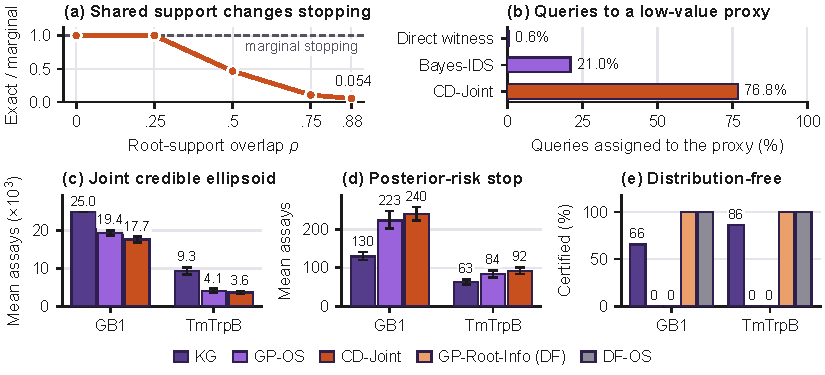
\includegraphics{figures/fig2_main_results.pdf}
\vspace{-12pt}
\caption{\textbf{Tasks, decision-relevant information, and the role of the stopping rule.}
\textbf{(a)} Simulated search graphs: each root action reaches private terminals and
terminals shared by all actions (fraction $\rho$).
\textbf{(b)} Protein engineering: the first substitution is the root action, and
different mutation orders reach the same measured variant.
\textbf{(c)} Agentic workflows: one module per stage gives $3^4=81$ workflows,
executed by Qwen3-0.6B and scored by graph $F_1$.
\textbf{(d)} Exact versus marginal stopping on identical passive
TA-UCT Bernoulli traces, $M=256$
(Table~\ref{tab:exact-regret-overlap}).
\textbf{(e)} Measurements assigned to a suboptimal but informative
proxy in a separate $M=5,d=3$ correlated experiment
(Table~\ref{tab:app-e0}).
\textbf{(f--h)} Measured GB1 ($n=200$) and TmTrpB ($n=210$) campaigns,
$\varepsilon=.015$, $\delta=.05$, $25$k cap; bars show $95\%$ intervals.
\textbf{(f)} Joint Gaussian credible-ellipsoid stopping.
\textbf{(g)} Direct working-posterior risk on frozen acquisition
trajectories.
\textbf{(h)} Independent-arm anytime-valid confidence sequences;
DF-aware GP-Root-Info and DF-OS both complete all campaigns
(Table~\ref{tab:app-v13-regime-b}).
The working GP is not empirically calibrated at the nominal
joint coverage level.}
\label{fig:main-results}
\end{figure}


\subsection{Protein Sequence Optimization under Epistasis}
\label{sec:exp-proteins}\label{sec:exp-real-world}

\paragraph{Certifying mutations in combinatorial landscapes.}
Allowing twenty amino acids at four positions yields
$20^4=160{,}000$ possible protein sequences. Moreover, epistasis
makes the effect of a substitution dependent on its sequence
background \citep{wu2016gb1,poelwijk2019epistasis}.
The TrpB landscape alone contains $519$ suboptimal single-mutation
local optima, nine requiring three simultaneous substitutions
to reach an improving neighbor \citep{johnston2024trpb}.
The immediate fitness of a mutation therefore need not reflect
the quality of its attainable continuations.

Using measured four-site GB1 and TmTrpB fitness landscapes
\citep{wu2016gb1,johnston2024trpb,dallago2021flip},
we construct canonical DAGs of up to three successive substitutions
at distinct positions. The first mutation defines the root action,
while different subsequent mutation orders can reach shared outcomes
(Figure~\ref{fig:main-results}b).
We simulate noisy assays against published fitness measurements,
rather than conducting new wet-lab experiments.
The matched study uses ten GB1 templates ($20$ seeds each;
$n=200$) and all $21$ TmTrpB templates ($10$ seeds each;
$n=210$), with a common fixed sequence-kernel GP, paired
query-noise tapes, $\varepsilon=.015$, $\delta=.05$,
and a $25$k cap (Appendices~\ref{app:v13-protein}
and~\ref{app:v14-protein-credible}).

\paragraph{Decision-directed acquisition on measured landscapes.}
We first compare acquisition under a common joint posterior credible
ellipsoid of contrast rank $r=M-1$, with radius
$\beta=\sqrt{\chi^2_{r,.95}}$ also used by CD-Joint and GP-OS
for acquisition. On TmTrpB, CD-Joint certifies all campaigns
in $3{,}629$ restricted mean assays versus KG's $9{,}337$
($85.7\%$ completed), a $2.57\times$ reduction
(95\% paired CI $[2.51,2.64]$). On GB1, CD-Joint certifies
$70\%$ versus $63\%$ for GP-OS and $0\%$ for KG.
The acquisition advantage thus extends to epistatic landscapes
under the shared working Gaussian model.


\paragraph{Acquisition efficiency depends on the stopping criterion.}
Changing the evidence required to stop reverses the acquisition
ranking (Figure~\ref{fig:main-results}f--h).
Under direct posterior-risk stopping, evaluated using a
time-and-action-uniform Monte Carlo approximation on frozen
trajectories, KG stops earlier than ellipsoid-directed CD-Joint
($130$ versus $240$ assays on GB1; $63$ versus $92$ on TmTrpB).
Under independent-arm distribution-free (DF) stopping, GP-only
CD-Joint and GP-OS certify no campaigns by $25$k, whereas
DF-coupled GP-Root-Info and DF-OS certify all campaigns.

These findings are consistent with the theoretical distinction
between stopping objectives: reducing worst-case regret over
a joint uncertainty set is not equivalent to reducing posterior
decision risk, and correlated observations need not contract
independent-arm confidence sequences. Acquisition and stopping
should therefore be designed jointly.

\begin{table}[t]
\centering\small
\caption{\textbf{Protein certification under different stopping rules.}
Restricted mean capped assays [completion \%], $B=25{,}000$.
The joint ellipsoid and posterior-risk criteria are model-based;
observed posterior-risk decision errors range from $1.5$ to $5.2\%$.
$^*$ denotes entirely capped cohorts.}
\label{tab:main-protein-summary}
\setlength{\tabcolsep}{4.5pt}
\begin{tabular}{@{}llrrr@{}}
\toprule
Landscape & Stopping criterion & Correlated KG & GP-OS & CD-Joint \\
\midrule
GB1 & $95\%$ joint ellipsoid & $25{,}000^*$ [$0\%$] & $19{,}450$ [$63\%$] & $\mathbf{17{,}678}$ [$70\%$] \\
TmTrpB & $95\%$ joint ellipsoid & $9{,}337$ [$85.7\%$] & $4{,}122$ [$100\%$] & $\mathbf{3{,}629}$ [$100\%$] \\
\midrule
GB1 & Direct posterior risk & $\mathbf{130}$ [$100\%$] & $223$ [$100\%$] & $240$ [$100\%$] \\
TmTrpB & Direct posterior risk & $\mathbf{63}$ [$100\%$] & $84$ [$100\%$] & $92$ [$100\%$] \\
\midrule
GB1 & Independent-arm DF & $20{,}102$ [$65.5\%$] & $25{,}000^*$ [$0\%$] & $25{,}000^*$ [$0\%$] \\
TmTrpB & Independent-arm DF & $17{,}184$ [$85.7\%$] & $25{,}000^*$ [$0\%$] & $25{,}000^*$ [$0\%$] \\
\bottomrule
\end{tabular}
\vspace{-3pt}
\end{table}

\paragraph{Calibration and external validity.}
Although the Gaussian contrast ellipsoid has nominal posterior
coverage of $95\%$, empirical joint coverage ranges from $45.7\%$
to $84.3\%$. The rank correction increases the radius from roughly
$7$ (with $0\%$ joint coverage) to $23$--$25$
(Appendix~\ref{app:v14-protein-credible}).
No decision errors are observed under the corrected ellipsoid,
whereas direct posterior-risk stopping incurs $1.5$--$5.2\%$
errors. Neither establishes frequentist GP coverage.
Interestingly, a separate empirical-Bayes study finds simultaneous
terminal-wise coverage of $91.5\%$ (GB1) and $82.9\%$ (TmTrpB),
yet $100\%$ empirical root-regret-bound coverage across $410$
campaigns (Appendix~\ref{app:v11-audit}). This motivates
calibrating uncertainty directly at the decision level.


\subsection{Agentic Workflow Configuration}
\label{sec:exp-workflows}

\paragraph{Certifying decisions under expensive evaluation.}
Whereas protein engineering illustrates large combinatorial
landscapes, agentic workflow design provides a complementary
setting in which individual evaluations are expensive.
Tool representation, planning, decoding, and verification
choices interact, motivating partial commitments rather than
immediate optimization of complete workflows
\citep{zhang2025aflow}. Different orders of component selection
can reach the same configuration, yielding overlapping supports.

We use WorFBench \citep{qiao2025worfbench} with three options
for each of four configuration stages, producing $3^4=81$
workflows evaluated by graph-workflow $F_1$ (Figure~\ref{fig:main-results}c).
In the offline, replay-accounted study, Optimistic Separation
(OS) certifies $100\%$ of campaigns using $1{,}937$ median
evaluations and $0.95$ million accounted tokens, compared with
$73.3\%$, $8{,}486$ evaluations, and $4.78$ million tokens for
Flat-LUCB with root stopping. Both attain held-out $F_1=0.529$:
shared-support allocation achieves the same observed held-out
performance using approximately one-fifth of the accounted tokens.
The DF interpretation remains conditional on independent
task sampling with replacement, which is not verified in the
available experimental record
(Appendix~\ref{sec:real-world-appendix}).

\paragraph{Fresh inference and statistical guarantees.}
A separate replication performs fresh, uncached Qwen3-0.6B
inference across $36$ campaigns and four domains, with a cap
of $60$ evaluations. Bounded-observation OS and GP-guided
acquisition with DF stopping certify $0/36$ campaigns.
Empirical-Bayes acquisition with leave-one-out-inflated GP
stopping certifies $36/36$ in a median of $24$ evaluations,
consuming $14{,}291$ fresh tokens versus OS's capped $26{,}862$,
with held-out $F_1$ of $0.4717$ versus $0.4172$.
These results illustrate the practical trade-off between
experimental cost and statistical guarantees: model-based
certification can stop earlier, but does not inherit DF validity.

\begin{table}[H]
\centering\small
\caption{\textbf{WorFBench: shared-support certification and uncached execution.}
Offline and live cohorts have different task pools and budgets.
DF denotes bounded-stream stopping, conditional on the stated
sampling assumptions; EB denotes empirically calibrated GP stopping.
See Tables~\ref{tab:main-applications},
\ref{tab:app-worfbench-domains}, and~\ref{tab:app-v11-live36}.}
\label{tab:main-worfbench}
\setlength{\tabcolsep}{4pt}
\begin{tabular}{@{}llrrrr@{}}
\toprule
Cohort & Method & Certified & Evals & Tokens & Held-out $F_1$\\
\midrule
Offline & Flat+Root (DF) & $73.3\%$ & $8{,}486$ & $4.78$ M & $.529$\\
Offline & OS (DF) & $100\%$ & $1{,}937$ & $0.95$ M & $.529$\\
\midrule
Live & OS (DF) & $0/36$ & $60^*$ & $26{,}862^*$ & $.4172$\\
Live & GP+DF & $0/36$ & $60^*$ & $31{,}808^*$ & $.4542$\\
Live & EB+LOO & $36/36$ & $24$ & $14{,}291$ & $.4717$\\
\bottomrule
\end{tabular}
\end{table}

\section{Outlook}
\label{sec:discussion}
Root-action identification is classical; our contribution is to determine which shared, correlated uncertainties can invalidate a commitment. On an all-MAX DAG, common-environment regret cancels shared outcomes, yielding sparse outside--inside contrasts and the CD-Joint acquisition rule. Under matched Gaussian beliefs and stopping, this reduces certification cost against KG; an anytime-valid fixed-feature study confirms a corresponding gain. On measured proteins, the corrected GP contrast ellipsoid retains a substantial empirical advantage under the working model.

The stopping-rule experiments also identify the limits of this advantage. KG stops faster under direct posterior-risk stopping, whereas independent-arm distribution-free confidence sequences require exploration beyond that induced by GP-only CD-Joint. Correct Gaussian credible geometry does not ensure calibration on measured fitness landscapes. Future work should couple decision-calibrated evidence with acquisition robust to misspecification and extend beyond finite, known all-MAX graphs to stochastic transitions, adversarial choices, or unknown reachable supports. The general principle is to measure uncertainty that can change a commitment and certify it with evidence appropriate to the observation model.
\label{main:lastpage}


\section*{AI Use Statement}
Generative AI tools assisted with literature synthesis,
theoretical development, proof generation, experimental
implementation, and manuscript preparation. Accompanying
Lean formalizations are provided in the \texttt{lean/}
directory of the source repository. The authors retain
full responsibility for the correctness and integrity
of all theoretical and empirical results.


\section*{Reproducibility Statement}

The source code accompanying this work, including algorithmic
implementations, experimental configurations, evaluation
scripts, numerical verification routines, and Lean
formalizations, is available at
\url{https://github.com/AI-MathPhys/dag-cert}.
%
The supplementary material provides detailed mathematical
proofs, statistical assumptions, experimental protocols,
extended results, and computational analyses. The
\texttt{lean/} directory contains a Lean~4 formalization
(Lean and Mathlib \texttt{v4.36.0}) of all $62$ numbered
theorems, lemmas, propositions and corollaries, each proved
as stated here, with no \texttt{sorry} and no axioms beyond
Lean's standard \texttt{propext}, \texttt{Classical.choice}
and \texttt{Quot.sound}. The file
\texttt{lean/JointRootCert/Manuscript.lean} restates every
result under its label in this paper, \texttt{lake build}
reproduces the proofs, a script checks their axioms, and
\texttt{lean/README.md} records for each result how the
formal statement models the text.

\begin{thebibliography}{99}

\bibitem[Abbasi-Yadkori et~al.(2011)Abbasi-Yadkori, P\'al, and Szepesv\'ari]{abbasi2011}
Yasin Abbasi-Yadkori, D\'avid P\'al, and Csaba Szepesv\'ari.
Improved algorithms for linear stochastic bandits.
In \emph{Advances in Neural Information Processing Systems 24}, pp.\ 2312--2320, 2011.
\url{https://proceedings.neurips.cc/paper/2011/hash/e1d5be1c7f2f456670de3d53c7b54f4a-Abstract.html}.

\bibitem[Bogunovic et~al.(2016)Bogunovic, Scarlett, Krause, and Cevher]{bogunovic2016truvar}
Ilija Bogunovic, Jonathan Scarlett, Andreas Krause, and Volkan Cevher.
Truncated variance reduction: A unified approach to Bayesian optimization and level-set estimation.
In \emph{Advances in Neural Information Processing Systems 29}, 2016.
\url{https://proceedings.neurips.cc/paper/2016/hash/ce78d1da254c0843eb23951ae077ff5f-Abstract.html}.

\bibitem[Boutilier et~al.(2006)Boutilier, Patrascu, Poupart, and Schuurmans]{boutilier2006minimax}
Craig Boutilier, Relu Patrascu, Pascal Poupart, and Dale Schuurmans.
Constraint-based optimization and utility elicitation using the minimax decision criterion.
\emph{Artificial Intelligence}, 170(8--9):686--713, 2006.
\url{https://doi.org/10.1016/j.artint.2006.02.003}.

\bibitem[Chaloner and Verdinelli(1995)]{chaloner1995design}
Kathryn Chaloner and Isabella Verdinelli.
Bayesian experimental design: A review.
\emph{Statistical Science}, 10(3):273--304, 1995.
\url{https://doi.org/10.1214/ss/1177009939}.

\bibitem[Chen et~al.(2014)Chen, Lin, King, Lyu, and Chen]{chen2014combinatorial}
Shouyuan Chen, Tian Lin, Irwin King, Michael R. Lyu, and Wei Chen.
Combinatorial pure exploration of multi-armed bandits.
In \emph{Advances in Neural Information Processing Systems 27}, pp.\ 379--387, 2014.
\url{https://proceedings.neurips.cc/paper_files/paper/2014/hash/d3ea0f3316d2da934d79b8b344eafee4-Abstract.html}.

\bibitem[Childs et~al.(2008)Childs, Brodeur, and Kocsis]{childs2008transpositions}
Benjamin E. Childs, James H. Brodeur, and Levente Kocsis.
Transpositions and move groups in Monte Carlo tree search.
In \emph{IEEE Symposium on Computational Intelligence and Games}, 2008.
\url{https://doi.org/10.1109/CIG.2008.5035667}.

\bibitem[Chowdhury and Gopalan(2017)]{chowdhury2017kernelized}
Sayak Ray Chowdhury and Aditya Gopalan.
On kernelized multi-armed bandits.
In \emph{Proceedings of ICML}, volume 70 of PMLR, pp.\ 844--853, 2017.
\url{https://proceedings.mlr.press/v70/chowdhury17a.html}.

\bibitem[Czech et~al.(2021)Czech, Korus, and Kersting]{czech2021mcgs}
Johannes Czech, Patrick Korus, and Kristian Kersting.
Improving AlphaZero using Monte-Carlo graph search.
In \emph{Proceedings of ICAPS}, pp.\ 103--111, 2021.
\url{https://doi.org/10.1609/icaps.v31i1.15952}.

\bibitem[Dallago et~al.(2021)Dallago, Mou, Johnston, Wittmann, Bhattacharya, Goldman, Madani, and Yang]{dallago2021flip}
Christian Dallago, Jody Mou, Kadina E. Johnston, Bruce Wittmann, Nicholas Bhattacharya, Samuel Goldman, Ali Madani, and Kevin K. Yang.
FLIP: Benchmark tasks in fitness landscape inference for proteins.
In \emph{NeurIPS Datasets and Benchmarks}, 2021.
\url{https://datasets-benchmarks-proceedings.neurips.cc/paper/2021/hash/2b44928ae11fb9384c4cf38708677c48-Abstract-round2.html}.

\bibitem[Dam et~al.(2025)Dam, Stenger, Schneider, Pajarinen, D'Eramo, and Maillard]{dam2025wasserstein}
Tuan Quang Dam, Pascal Stenger, Lukas Schneider, Joni Pajarinen, Carlo D'Eramo, and Odalric-Ambrym Maillard.
Monte-Carlo tree search with uncertainty propagation via optimal transport.
In \emph{Proceedings of ICML}, volume 267 of PMLR, pp.\ 12377--12401, 2025.
\url{https://proceedings.mlr.press/v267/dam25c.html}.

\bibitem[Degenne and Koolen(2019)]{degenne2019multiple}
R\'emy Degenne and Wouter M. Koolen.
Pure exploration with multiple correct answers.
In \emph{Advances in Neural Information Processing Systems 32}, 2019.
\url{https://papers.nips.cc/paper_files/paper/2019/hash/60cb558c40e4f18479664069d9642d5a-Abstract.html}.

\bibitem[Degenne et~al.(2020)Degenne, M\'enard, Shang, and Valko]{degenne2020gamification}
R\'emy Degenne, Pierre M\'enard, Xuedong Shang, and Michal Valko.
Gamification of pure exploration for linear bandits.
In \emph{Proceedings of ICML}, volume 119 of PMLR, pp.\ 2432--2442, 2020.
\url{https://proceedings.mlr.press/v119/degenne20a.html}.

\bibitem[Drton(2008)]{drton2008}
Mathias Drton.
Multiple solutions to the likelihood equations in the Behrens--Fisher problem.
\emph{Statistics \& Probability Letters}, 78(18):3288--3293, 2008.
\url{https://doi.org/10.1016/j.spl.2008.06.012}.

\bibitem[Du et~al.(2021)Du, Kuroki, and Chen]{du2021partial}
Yihan Du, Yuko Kuroki, and Wei Chen.
Combinatorial pure exploration with full-bandit or partial linear feedback.
In \emph{Proceedings of AAAI}, pp.\ 7262--7270, 2021.
\url{https://doi.org/10.1609/AAAI.V35I8.16892}.

\bibitem[Fiez et~al.(2019)Fiez, Jain, Jamieson, and Ratliff]{fiez2019}
Tanner Fiez, Lalit Jain, Kevin G. Jamieson, and Lillian Ratliff.
Sequential experimental design for transductive linear bandits.
In \emph{Advances in Neural Information Processing Systems 32}, 2019.
\url{https://proceedings.neurips.cc/paper/2019/hash/8ba6c657b03fc7c8dd4dff8e45defcd2-Abstract.html}.

\bibitem[Filstroff et~al.(2024)Filstroff, Sundin, Mikkola, Tiulpin, Kylm\"aoja, and Kaski]{filstroff2024targeted}
Louis Filstroff, Iiris Sundin, Petrus Mikkola, Aleksei Tiulpin, Juuso Kylm\"aoja, and Samuel Kaski.
Targeted active learning for Bayesian decision-making.
\emph{Transactions on Machine Learning Research}, 2024.
\url{https://mlanthology.org/tmlr/2024/filstroff2024tmlr-targeted/}.

\bibitem[Frazier et~al.(2009)Frazier, Powell, and Dayanik]{frazier2009kg}
Peter Frazier, Warren Powell, and Savas Dayanik.
The knowledge-gradient policy for correlated normal beliefs.
\emph{INFORMS Journal on Computing}, 21(4):599--613, 2009.
\url{https://doi.org/10.1287/ijoc.1080.0314}.

\bibitem[Gabillon et~al.(2012)Gabillon, Ghavamzadeh, and Lazaric]{gabillon2012best}
Victor Gabillon, Mohammad Ghavamzadeh, and Alessandro Lazaric.
Best arm identification: A unified approach to fixed budget and fixed confidence.
In \emph{Advances in Neural Information Processing Systems 25}, 2012.
\url{https://papers.nips.cc/paper_files/paper/2012/hash/8b0d268963dd0cfb808aac48a549829f-Abstract.html}.

\bibitem[Garivier and Kaufmann(2016)]{garivier2016optimal}
Aur\'elien Garivier and Emilie Kaufmann.
Optimal best arm identification with fixed confidence.
In \emph{Proceedings of COLT}, volume 49 of PMLR, pp.\ 998--1027, 2016.
\url{https://proceedings.mlr.press/v49/garivier16a.html}.

\bibitem[Go et~al.(2026)Go, Qian, and Yoon]{go2026goal}
Jinwoo Go, Xiaoning Qian, and Byung-Jun Yoon.
Goal-driven Bayesian optimal experimental design for robust decision-making under model uncertainty.
\emph{arXiv preprint arXiv:2605.26093}, 2026.
\url{https://arxiv.org/abs/2605.26093}.

\bibitem[Hennig and Schuler(2012)]{hennig2012entropy}
Philipp Hennig and Christian J. Schuler.
Entropy search for information-efficient global optimization.
\emph{Journal of Machine Learning Research}, 13(57):1809--1837, 2012.
\url{https://jmlr.org/papers/v13/hennig12a.html}.

\bibitem[Hern\'andez-Lobato et~al.(2014)Hern\'andez-Lobato, Hoffman, and Ghahramani]{hernandez2014pes}
Jos\'e Miguel Hern\'andez-Lobato, Matthew W. Hoffman, and Zoubin Ghahramani.
Predictive entropy search for efficient global optimization of black-box functions.
In \emph{Advances in Neural Information Processing Systems 27}, 2014.
\url{https://proceedings.neurips.cc/paper_files/paper/2014/hash/6488484c982e9af5c35689523ba1abfe-Abstract.html}.

\bibitem[Hoffman et~al.(2014)Hoffman, Shahriari, and de Freitas]{hoffman2014bayesgap}
Matthew W. Hoffman, Bobak Shahriari, and Nando de Freitas.
On correlation and budget constraints in model-based bandit optimization with application to automatic machine learning.
In \emph{Proceedings of AISTATS}, volume 33 of PMLR, pp.\ 365--374, 2014.
\url{https://proceedings.mlr.press/v33/hoffman14.html}.

\bibitem[Howard et~al.(2021)Howard, Ramdas, McAuliffe, and Sekhon]{howard}
Steven R. Howard, Aaditya Ramdas, Jon McAuliffe, and Jasjeet Sekhon.
Time-uniform, nonparametric, nonasymptotic confidence sequences.
\emph{The Annals of Statistics}, 49(2):1055--1080, 2021.
\url{https://doi.org/10.1214/20-AOS1991}.

\bibitem[Huang et~al.(2017)Huang, Ajallooeian, Szepesv\'ari, and M\"uller]{huang}
Ruitong Huang, Mohammad M. Ajallooeian, Csaba Szepesv\'ari, and Martin M\"uller.
Structured best arm identification with fixed confidence.
In \emph{Proceedings of ALT}, volume 76 of PMLR, pp.\ 593--616, 2017.
\url{https://proceedings.mlr.press/v76/huang17a.html}.

\bibitem[Huang et~al.(2024)Huang, Guo, Acerbi, and Kaski]{huang2024amortized}
Daolang Huang, Yujia Guo, Luigi Acerbi, and Samuel Kaski.
Amortized Bayesian experimental design for decision-making.
In \emph{Advances in Neural Information Processing Systems 37}, pp.\ 109460--109486, 2024.
\url{https://proceedings.neurips.cc/paper_files/paper/2024/hash/c59f05d7ab3638b138cc61f32e1a7cd1-Abstract-Conference.html}.

\bibitem[Jang et~al.(2024)Jang, Komiyama, and Yamazaki]{jang2024bayesian}
Kyoungseok Jang, Junpei Komiyama, and Kazutoshi Yamazaki.
Fixed confidence best arm identification in the Bayesian setting.
In \emph{Advances in Neural Information Processing Systems 37}, 2024.
\url{https://papers.nips.cc/paper/2024/hash/1fb0a4de9c14f5557eeea886e22569cd-Abstract-Conference.html}.

\bibitem[Jedra and Proutiere(2020)]{jedra2020linear}
Yassir Jedra and Alexandre Proutiere.
Optimal best-arm identification in linear bandits.
In \emph{Advances in Neural Information Processing Systems 33}, 2020.
\url{https://proceedings.neurips.cc/paper/2020/hash/7212a6567c8a6c513f33b858d868ff80-Abstract.html}.

\bibitem[Jin et~al.(2024)Jin, Yang, Tang, Xiao, and Xu]{jin2024batched}
Tianyuan Jin, Yu Yang, Jing Tang, Xiaokui Xiao, and Pan Xu.
Optimal batched best arm identification.
In \emph{Advances in Neural Information Processing Systems 37 (NeurIPS)}, 2024.

\bibitem[Johnston et~al.(2024)Johnston, Almhjell, Watkins-Dulaney, Liu, Porter, Yang, and Arnold]{johnston2024trpb}
Kadina E. Johnston, Patrick J. Almhjell, Ella J. Watkins-Dulaney, Grace Liu, Nicholas J. Porter, Jason Yang, and Frances H. Arnold.
A combinatorially complete epistatic fitness landscape in an enzyme active site.
\emph{Proceedings of the National Academy of Sciences}, 121(32):e2400439121, 2024.
\url{https://doi.org/10.1073/pnas.2400439121}.

\bibitem[Jourdan and Degenne(2022)]{jourdan2022answers}
Marc Jourdan and R\'emy Degenne.
Choosing answers in epsilon-best-answer identification for linear bandits.
In \emph{Proceedings of ICML}, volume 162 of PMLR, pp.\ 10384--10430, 2022.
\url{https://proceedings.mlr.press/v162/jourdan22a.html}.

\bibitem[Jourdan et~al.(2023)Jourdan, Degenne, and Kaufmann]{jourdan2023unknown}
Marc Jourdan, R\'emy Degenne, and Emilie Kaufmann.
Dealing with unknown variances in best-arm identification.
In \emph{Proceedings of ALT}, volume 201 of PMLR, pp.\ 776--849, 2023.
\url{https://proceedings.mlr.press/v201/jourdan23a.html}.

\bibitem[Kalyanakrishnan et~al.(2012)Kalyanakrishnan, Tewari, Auer, and Stone]{kalyanakrishnan2012pac}
Shivaram Kalyanakrishnan, Ambuj Tewari, Peter Auer, and Peter Stone.
PAC subset selection in stochastic multi-armed bandits.
In \emph{Proceedings of ICML}, pp.\ 655--662, 2012.
\url{https://www.cs.utexas.edu/~shivaram/papers/ktas_icml_2012.pdf}.

\bibitem[Kaufmann et~al.(2016)Kaufmann, Capp\'e, and Garivier]{kaufmannkl}
Emilie Kaufmann, Olivier Capp\'e, and Aur\'elien Garivier.
On the complexity of best-arm identification in multi-armed bandit models.
\emph{Journal of Machine Learning Research}, 17(1):1--42, 2016.
\url{https://jmlr.org/papers/v17/kaufman16a.html}.

\bibitem[Kaufmann and Koolen(2017)]{kaufmann}
Emilie Kaufmann and Wouter M. Koolen.
Monte-Carlo tree search by best arm identification.
In \emph{Advances in Neural Information Processing Systems 30}, 2017.
\url{https://arxiv.org/abs/1706.02986}.

\bibitem[Kirschner et~al.(2020)Kirschner, Lattimore, and Krause]{kirschner2020ids}
Johannes Kirschner, Tor Lattimore, and Andreas Krause.
Information directed sampling for linear partial monitoring.
In \emph{Proceedings of COLT}, volume 125 of PMLR, pp.\ 2328--2369, 2020.
\url{https://proceedings.mlr.press/v125/kirschner20a.html}.

\bibitem[Kocsis and Szepesv\'ari(2006)]{uctoriginal}
Levente Kocsis and Csaba Szepesv\'ari.
Bandit based Monte-Carlo planning.
In \emph{Machine Learning: ECML 2006}, pp.\ 282--293, 2006.
\url{https://doi.org/10.1007/11871842_29}.

\bibitem[Kujanp\"a\"a et~al.(2024)Kujanp\"a\"a, Babadi, Zhao, Kannala, Ilin, and Pajarinen]{kujanpaa2024cmcgs}
Kalle Kujanp\"a\"a, Amin Babadi, Yi Zhao, Juho Kannala, Alexander Ilin, and Joni Pajarinen.
Continuous Monte Carlo graph search.
In \emph{Proceedings of AAMAS}, pp.\ 1047--1056, 2024.
\url{https://doi.org/10.5555/3635637.3662960}.

\bibitem[Laurent and Massart(2000)]{laurent2000}
B\'eatrice Laurent and Pascal Massart.
Adaptive estimation of a quadratic functional by model selection.
\emph{The Annals of Statistics}, 28(5):1302--1338, 2000.
\url{https://doi.org/10.1214/aos/1015957395}.

\bibitem[Luong et~al.(2026)Luong, Nguyen, Ta, Tran, and Dam]{luong2026varde}
Khang Luong, Nam Nguyen, Hoang Ta, Hung The Tran, and Tuan Quang Dam.
Variance driven exploration: A provable and efficient methodology for pure exploration in highly stochastic environments.
In \emph{Proceedings of ICML}, volume 306 of PMLR, pp.\ 83248--83283, 2026.
\url{https://proceedings.mlr.press/v306/luong26a.html}.

\bibitem[Maurer and Pontil(2009)]{maurer2009empirical}
Andreas Maurer and Massimiliano Pontil.
Empirical Bernstein bounds and sample variance penalization.
In \emph{Proceedings of COLT}, 2009.
\url{https://arxiv.org/abs/0907.3740}.

\bibitem[P\'elissier et~al.(2019)P\'elissier, Nakamura, and Tabata]{pelissier}
Aur\'elien P\'elissier, Atsuyoshi Nakamura, and Koji Tabata.
Feature selection as Monte-Carlo search in growing single rooted directed acyclic graph by best leaf identification.
In \emph{Proceedings of the SIAM International Conference on Data Mining}, pp.\ 450--458, 2019.
\url{https://doi.org/10.1137/1.9781611975673.51}.

\bibitem[Poelwijk et~al.(2019)Poelwijk, Socolich, and Ranganathan]{poelwijk2019epistasis}
Frank J. Poelwijk, Michael Socolich, and Rama Ranganathan.
Learning the pattern of epistasis linking genotype and phenotype in a protein.
\emph{Nature Communications}, 10:4213, 2019.
\url{https://doi.org/10.1038/s41467-019-12130-8}.

\bibitem[Poursoltani and Delage(2022)]{poursoltani2022regret}
Mehran Poursoltani and Erick Delage.
Adjustable robust optimization reformulations of two-stage worst-case regret minimization problems.
\emph{Operations Research}, 70(5):2906--2930, 2022.
\url{https://www.gerad.ca/en/papers/G-2019-56}.

\bibitem[Qiao et~al.(2025)Qiao, Fang, Qiu, Wang, Zhang, Jiang, Xie, Huang, and Chen]{qiao2025worfbench}
Shuofei Qiao, Runnan Fang, Zhisong Qiu, Xiaobin Wang, Ningyu Zhang, Yong Jiang, Pengjun Xie, Fei Huang, and Huajun Chen.
Benchmarking agentic workflow generation.
In \emph{Proceedings of ICLR}, 2025.
\url{https://arxiv.org/abs/2410.07869}.

\bibitem[Sion(1958)]{sion1958}
Maurice Sion.
On general minimax theorems.
\emph{Pacific Journal of Mathematics}, 8(1):171--176, 1958.
\url{https://doi.org/10.2140/pjm.1958.8.171}.

\bibitem[Qin and You(2026)]{qin2026dual}
Chao Qin and Wei You.
Dual-directed algorithm design for efficient pure exploration.
\emph{Operations Research}, 74(2):1104--1125, 2026.
\url{https://doi.org/10.1287/opre.2023.0590}.

\bibitem[Russo and Van Roy(2018)]{russo2018ids}
Daniel Russo and Benjamin Van Roy.
Learning to optimize via information-directed sampling.
\emph{Operations Research}, 66(1):230--252, 2018.
\url{https://doi.org/10.1287/opre.2017.1663}.

\bibitem[Saffidine et~al.(2012)Saffidine, Cazenave, and M\'ehat]{saffidine2012ucd}
Abdallah Saffidine, Tristan Cazenave, and Jean M\'ehat.
UCD: Upper confidence bound for rooted directed acyclic graphs.
\emph{Knowledge-Based Systems}, 34:26--33, 2012.
\url{https://doi.org/10.1016/j.knosys.2011.11.014}.

\bibitem[Shang et~al.(2020)Shang, de Heide, M\'enard, Kaufmann, and Valko]{shang2020bayesian}
Xuedong Shang, Rianne de Heide, Pierre M\'enard, Emilie Kaufmann, and Michal Valko.
Fixed-confidence guarantees for Bayesian best-arm identification.
In \emph{Proceedings of AISTATS}, volume 108 of PMLR, pp.\ 1823--1832, 2020.
\url{https://proceedings.mlr.press/v108/shang20a.html}.

\bibitem[Soare et~al.(2014)Soare, Lazaric, and Munos]{soare2014linear}
Marta Soare, Alessandro Lazaric, and R\'emi Munos.
Best-arm identification in linear bandits.
In \emph{Advances in Neural Information Processing Systems 27}, 2014.
\url{https://proceedings.neurips.cc/paper_files/paper/2014/hash/f8d84caae48546d0934d637ab54f7086-Abstract.html}.

\bibitem[Srinivas et~al.(2012)Srinivas, Krause, Kakade, and Seeger]{srinivas2012gpucb}
Niranjan Srinivas, Andreas Krause, Sham M. Kakade, and Matthias Seeger.
Information-theoretic regret bounds for Gaussian process optimization in the bandit setting.
\emph{IEEE Transactions on Information Theory}, 58(5):3250--3265, 2012.
\url{https://doi.org/10.1109/TIT.2011.2182033}.

\bibitem[Tesauro et~al.(2010)Tesauro, Rajan, and Segal]{tesauro2010bayesian}
Gerald Tesauro, V. T. Rajan, and Richard Segal.
Bayesian inference in Monte-Carlo tree search.
In \emph{Proceedings of UAI}, pp.\ 587--595, 2010.
\url{https://proceedings.mlr.press/r8/tesauro10a.html}.

\bibitem[Tuynman and Degenne(2025)]{tuynman2025batch}
Adrienne Tuynman and R\'emy Degenne.
The batch complexity of bandit pure exploration.
In \emph{Proceedings of ICML}, volume 267 of PMLR, pp.\ 60442--60468, 2025.
\url{https://proceedings.mlr.press/v267/tuynman25a.html}.

\bibitem[Wang and Scarlett(2022)]{wang2022grouped}
Zhenlin Wang and Jonathan Scarlett.
Max-min grouped bandits.
In \emph{Proceedings of AAAI}, pp.\ 8603--8611, 2022.
\url{https://doi.org/10.1609/AAAI.V36I8.20838}.

\bibitem[Waudby-Smith and Ramdas(2024)]{bettingmeans}
Ian Waudby-Smith and Aaditya Ramdas.
Estimating means of bounded random variables by betting.
\emph{Journal of the Royal Statistical Society Series B: Statistical Methodology}, 86(1):1--27, 2024.
\url{https://doi.org/10.1093/jrsssb/qkad009}.

\bibitem[Wilson(2024)]{wilson2024stopping}
James T. Wilson.
Stopping Bayesian optimization with probabilistic regret bounds.
In \emph{Advances in Neural Information Processing Systems 37}, 2024.
\url{https://proceedings.neurips.cc/paper_files/paper/2024/hash/b204de7078301292a8876a762eed3dcb-Abstract-Conference.html}.

\bibitem[Wu et~al.(2016)Wu, Dai, Olson, Lloyd-Smith, and Sun]{wu2016gb1}
Nicholas C. Wu, Lei Dai, C. Anders Olson, James O. Lloyd-Smith, and Ren Sun.
Adaptation in protein fitness landscapes is facilitated by indirect paths.
\emph{eLife}, 5:e16965, 2016.
\url{https://doi.org/10.7554/eLife.16965}.

\bibitem[Xie et~al.(2016)Xie, Frazier, and Chick]{xie2016correlated}
Jing Xie, Peter I. Frazier, and Stephen E. Chick.
Bayesian optimization via simulation with pairwise sampling and correlated prior beliefs.
\emph{Operations Research}, 64(2):542--559, 2016.
\url{https://doi.org/10.1287/opre.2016.1480}.

\bibitem[Xu et~al.(2018)Xu, Honda, and Sugiyama]{xu2018lingape}
Liyuan Xu, Junya Honda, and Masashi Sugiyama.
A fully adaptive algorithm for pure exploration in linear bandits.
In \emph{Proceedings of AISTATS}, volume 84 of PMLR, pp.\ 843--851, 2018.
\url{https://proceedings.mlr.press/v84/xu18d.html}.

\bibitem[Zhang et~al.(2025)Zhang, Xiang, Yu, Teng, Chen, Chen, Zhuge, Cheng, Hong, Wang, Zheng, Liu, Luo, and Wu]{zhang2025aflow}
Jiayi Zhang, Jinyu Xiang, Zhaoyang Yu, Fengwei Teng, Xiong-Hui Chen, Jiaqi Chen, Mingchen Zhuge, Xin Cheng, Sirui Hong, Jinlin Wang, Bingnan Zheng, Bang Liu, Yuyu Luo, and Chenglin Wu.
AFlow: Automating agentic workflow generation.
In \emph{Proceedings of ICLR}, 2025.
\url{https://arxiv.org/abs/2410.10762}.

\bibitem[Leurent and Maillard(2020)]{leurent2020graph}
Edouard Leurent and Odalric-Ambrym Maillard.
Monte-Carlo graph search: The value of merging similar states.
In \emph{Proceedings of ACML}, volume 129 of PMLR,
pp.\ 577--592, 2020.
\url{https://proceedings.mlr.press/v129/leurent20a.html}.

\bibitem[Tran et~al.(2026)Tran, Mai, Ta, and Dam]{tran2026graph}
Tung Tran, Viet Bao Mai, Hoang Ta, and Tuan Dam.
Graph-based stochastic Power-UCT: Monte-Carlo graph search
with power mean estimation.
\emph{arXiv preprint arXiv:2609.19956}, 2026.
\url{https://arxiv.org/abs/2609.19956}.

\bibitem[Nameki et~al.(2026)Nameki, Nakamura, Komiyama, and Tabata]
{nameki2026thresholding}
Shoma Nameki, Atsuyoshi Nakamura, Junpei Komiyama, and Koji Tabata.
An efficient algorithm for thresholding Monte Carlo tree search.
\emph{arXiv preprint arXiv:2601.22600}, 2026.
\url{https://arxiv.org/abs/2601.22600}.

\end{thebibliography}

\clearpage
\appendix
\section*{Supplementary Material}
\noindent
The supplementary material develops the theoretical, experimental,
and computational foundations of Joint Root Certification and
decision-directed experimental design. Part~I establishes the exact
geometry of root certification, derives acquisition guarantees,
characterizes statistical validity and information-theoretic limits,
and extends certification to passive graph-search trajectories.
Part~II presents the experimental methodology and complete results,
from controlled acquisition comparisons to protein fitness landscapes,
agentic workflows, and extended validation studies.
Part~III addresses computational implementation, numerical certification,
representation costs, and performance benchmarks.

Every numbered result below is also proved in Lean~4 in the
\texttt{lean/} directory of the accompanying source repository;
\texttt{lean/JointRootCert/Manuscript.lean} indexes the formal
statements by the labels used here, and \texttt{lean/README.md}
states, result by result, how each formal statement models the
text.

Throughout, we distinguish observation complexity from computational
cost, and formal statistical guarantees from empirical assessments
under working models. In particular, Bayesian acquisition does not
itself confer posterior or frequentist coverage. The corresponding
validity assumptions are collected in Section~\ref{app:group-robust}.

\paragraph{Guide to the main-text claims.}
The exact regret geometry and sparse ellipsoidal representation
are established in Section~\ref{app:group-cert}, while the
safeguarded acquisition rule and its finite-sample guarantees
are developed in Section~\ref{app:group-acquisition}.
Section~\ref{app:group-info} characterizes information-theoretic
limits through dedicated likelihood-certified tracking policies,
distinct from CD-Joint. The matched-model acquisition comparisons,
protein experiments, and workflow evaluations are presented in
Sections~\ref{app:group-results}, \ref{app:group-proteins}, and
\ref{app:group-workflows}, respectively.
Sections~\ref{app:group-compute} and~\ref{app:group-benchmarks}
describe the computational methods and independent numerical
verification.

% Appendix-only, hyperlinked contents. All numbered supplementary headings
% write to a separate contents file, without changing main-text numbering.
\makeatletter
\let\supp@original@addcontentsline\addcontentsline
\renewcommand{\addcontentsline}[3]{%
  \def\supp@file{#1}\def\supp@toc{toc}%
  \ifx\supp@file\supp@toc
    \supp@original@addcontentsline{stoc}{#2}{#3}%
  \else
    \supp@original@addcontentsline{#1}{#2}{#3}%
  \fi}
\newcommand{\supplementarycontents}{%
  \begingroup\setcounter{tocdepth}{2}\small\@starttoc{stoc}\endgroup}
\makeatother
\section*{Supplementary Contents}
\supplementarycontents

\clearpage
\phantomsection
\addcontentsline{stoc}{part}{Part I --- Theoretical Foundations}
\noindent{\Large\bfseries Part I --- Theoretical Foundations}\par\medskip
We separate deterministic decision geometry from acquisition, statistical coverage, and information complexity. All guarantees below retain their stated observation-access and model assumptions.

\section{Joint Root Certification: Exact Regret Geometry}
\label{app:group-cert}

Joint Root Certification evaluates the loss of an initial commitment under one common environment. We establish the general outside--inside reduction, its rectangular and ellipsoidal specializations, and the structural conditions under which no observations are required.

\subsection{Common-environment regret and shared-support cancellation}
\label{app:common-environment}\label{sec:bay-supp}

We begin with the joint-set reduction and the ellipsoidal minimax identity.  The finite action family has nonempty supports $S(a)$ whose
union is $Z$.  For $f_\theta(z)=\phi_z^\top\theta$, define
\[
 r_\theta(a)=\max_{z\in Z}\phi_z^\top\theta
              -\max_{y\in S(a)}\phi_y^\top\theta.
\]
The notation $R_C(a)=\sup_{\theta\in C}r_\theta(a)$ refers to robust
regret for a joint parameter set.  It is distinct from a marginal
confidence interval for an action value.

\begin{lemma}[Joint-set reduction]
\label{lem:bay-reduction}
For every nonempty compact $C$,
\[
 R_C(a)=\max\{0,\max_{z\notin S(a)}D_C(z,S(a))\},\qquad
 D_C(z,S)=\max_{\theta\in C}
       \min_{y\in S}(\phi_z-\phi_y)^\top\theta.
\]
The value is zero when the exterior is empty.
\end{lemma}
\begin{proof}
For any fixed parameter, the largest inside contribution to
$\max_z\phi_z^\top\theta-\max_{y\in S(a)}\phi_y^\top\theta$ is zero.
The remaining contributions come exactly from exterior terminals.
A supremum commutes with a finite maximum, proving the identity.
\end{proof}

\subsection{Exact rectangular certificates and anytime stopping}
\label{app:rect-proof}

\begin{theorem}[Exact rectangular shared-support certificate]
\label{thm:shared-regret}\label{thm:regret}
For every nonempty confidence box and proper root support, the robust regret equals the outside-support expression in~\eqref{eq:exact-robust-regret}. For full support it is zero.
\end{theorem}
\begin{corollary}[Anytime-valid root commitment]\label{cor:shared-regret-pac}
Under the simultaneous coverage condition~\eqref{eq:terminal-box}, returning any action with robust regret at most $\varepsilon$ incurs error probability at most $\delta$ for any predictable adaptive terminal-sampling policy.
\end{corollary}

The same outside-versus-inside reduction applies before specifying any uncertainty-set geometry. For a nonempty box, inside coordinates can be set to their lower endpoints and outside coordinates to their upper endpoints simultaneously.

\begin{proof}[Proof of \cref{thm:shared-regret} and \cref{cor:shared-regret-pac}]
Set $A(x)=\max_{z\in S(a)}x_z$ and $C(x)=\max_{z\notin S(a)}x_z$ when $Z\setminus S(a)\ne\emptyset$. Since every reachable terminal belongs to at least one root action's support, $\max_{b\in\mathcal A}\max_{z\in S(b)}x_z=\max\{A(x),C(x)\}$ and the point regret equals $[C(x)-A(x)]_+$, bounded above by $[\max_{z\notin S(a)}u_t(z)-L_t(a)]_+$. Setting $x_z=l_t(z)$ for $z\in S(a)$ and $x_z=u_t(z)$ for $z\notin S(a)$ attains this upper bound inside $\mathcal B_t$. If $S(a)=Z$, action $a$ is optimal for every $x\in\mathcal B_t$, giving $\mathcal R_t(a)=0$. Replacing $Z\setminus S(a)$ by $S(b)\setminus S(a)$ yields the pairwise identity. Equivalence with $\{z:u_t(z)>L_t(a)+\epsilon\}\subseteq S(a)$ and PAC soundness on $\mu\in\mathcal B_t$ follow immediately, and since every $z\notin S(a)$ lies in $S(b)$ for some $b\ne a$, $\max_{z\notin S(a)}u_t(z)\le \max_{b\ne a}U_t(b)$, proving~\eqref{eq:exact-robust-regret}.
\end{proof}

\subsection{Ellipsoidal minimax representation and sparse witnesses}
\label{app:ellipsoid-proofs}

\paragraph{Proof of \cref{thm:bay-main-dual}.}
Write $\theta=m+Lu$, $\|u\|_2\le\beta$, and set
$b_y=(\phi_z-\phi_y)^\top m$ and
$c_y=L^\top(\phi_z-\phi_y)$.  The bilinear function
$\sum_y p_y(b_y+c_y^\top u)$ is continuous on two compact convex sets.
The finite-dimensional convex minimax theorem \citep{sion1958} gives
\[
 \max_{\|u\|\le\beta}\min_y(b_y+c_y^\top u)
 =\min_{p\in\Delta(S)}\max_{\|u\|\le\beta}
       \sum_y p_y(b_y+c_y^\top u)
 =\min_{p\in\Delta(S)}
       \left[\sum_y p_yb_y+\beta\left\|\sum_y p_yc_y\right\|_2\right].
\]
All optima exist.  This proves the formula together with
\cref{lem:bay-reduction}, and requires no rank condition.

For sparsity, take a primal--dual optimal pair $(u_*,p_*)$.
Equality in weak duality implies that positive entries of $p_*$ occur
only where $b_y+c_y^\top u_*=D_C(z,S)$.  On this active set, preserving
$\sum_y p_yc_y$ also preserves $\sum_y p_yb_y$ and hence the objective.
The affine dimension of the active $c_y$ is at most $\operatorname{rank}(L)$.
Caratheodory's theorem therefore gives an equally good mixture supported
on at most $\operatorname{rank}(L)+1$ terms.  This bound is sharp: take
$L=I_r$, $m=0$, exterior feature zero, and inside features the vertices
of an $r$-simplex with zero in its interior.  A zero contrast requires
all $r+1$ vertices.  Finally, substituting any simplex vector into the
minimization gives an upper bound, establishing the numerical
certificate claim.\hfill$\square$

In particular, a feasible primal adversary gives a \emph{lower} regret
bound and cannot certify stopping.  In terminal coordinates,
$\phi_z=e_z$ and $K=LL^\top$ give
\[
 D_C(z,S)=\min_{p\in\Delta(S)}
 \left[m_z-p^\top m_S+
 \beta\sqrt{K_{zz}-2K_{zS}p+p^\top K_{SS}p}\right].
\]
The square-root representation enforces the affine support when $K$ is
singular; using a pseudoinverse inequality alone would incorrectly
leave null directions unrestricted.  For a fixed radius, adding
$\kappa\mathbf 1\mathbf 1^\top$ to $K$ leaves the formula unchanged,
because every contrast has zero coordinate sum.  If calibration changes
the radius when the rank changes, that statistical change must be treated
separately.  A diagonal covariance still defines an ellipsoid rather
than a Cartesian box, so comparisons must distinguish covariance from
confidence-set shape.

\subsection{Feature-hull dominance and structural screening}
\label{app:feature-hull}

\begin{theorem}[Feature-hull dominance]\label{thm:t2-hull}
Let $P_a=\conv\{\phi_y:y\in S(a)\}$ and $P_Z=\conv\{\phi_z:z\in Z\}$. Then $V(a;\theta)=V^*(\theta)$ for all $\theta\in\mathbb R^d$ if and only if $P_Z\subseteq P_a$. For a feature norm $\|\cdot\|$ and parameter dual norm $\|\cdot\|_*$, $\|\theta\|_*\le B$ implies regret at most $B\max_{z\notin S(a)}\inf_{p\in P_a}\|\phi_z-p\|$ (zero for an empty complement).
\end{theorem}

\begin{proof}[Proof of \cref{thm:t2-hull}]
If $P_Z\subseteq P_a$, every outside feature $\phi_z$ is a convex
combination of inside features and hence $\phi_z^\top\theta\le
\max_{y\in S(a)}\phi_y^\top\theta$ for every $\theta$. Conversely,
if some $\phi_z\notin P_a$, strict hyperplane separation supplies
$\theta$ for which $\phi_z^\top\theta>\max_{y\in S(a)}\phi_y^\top\theta$.
For the approximate statement choose $w_z\in P_a$ at distance at most
$\eta(a)$ from $\phi_z$ and apply H\"older's inequality to
$(\phi_z-w_z)^\top\theta$. Taking maxima completes the proof.
\end{proof}

\paragraph{Approximate feature-hull bound.}
For any outside $z$ and any $p\in P_a$, the maximum inside value is
at least $p^\top\theta$ because $p$ is a convex combination of inside
features. Therefore
\[
 \phi_z^\top\theta-\max_{y\in S(a)}\phi_y^\top\theta
 \le (\phi_z-p)^\top\theta
 \le\|\phi_z-p\|\,\|\theta\|_*,
\]
by dual-norm H\"older inequality. Infimizing over $p\in P_a$ and
maximizing over outside $z$ proves the bound of
Theorem~\ref{thm:t2-hull}; the empty-exterior case has zero regret.

\paragraph{Relation to structured root identification}

Classical MCTS and BAI-MCTS address root decisions in trees \citep{uctoriginal,kaufmann}; probabilistic MCTS propagates uncertainty and establishes asymptotic convergence \citep{tesauro2010bayesian,dam2025wasserstein}. Graph-based search has a substantial transposition literature \citep{childs2008transpositions,saffidine2012ucd,czech2021mcgs,kujanpaa2024cmcgs}. More directly, \citet{huang} formulate fixed-confidence identification of actions whose values are functions of shared micro-observables, explicitly accommodating transpositions, and \citet{pelissier} develop fixed-confidence root and leaf identification in growing DAGs. Our finite all-MAX support model is a specialization of the structured-payoff setting of \citet{huang} when terminal observations are independent. The distinction from marginal interval propagation is the exact common-environment bound, rather than the existence of a PAC search procedure. Max-min grouped bandits \citep{wang2022grouped} likewise exploit overlap, but maximize the minimum reward in a group. Their decision geometry differs from our maximum over retained continuations. General combinatorial and partial-linear-feedback pure exploration \citep{chen2014combinatorial,du2021partial} provide further related frameworks.

\clearpage

\section{Decision-Directed Experimental Design}
\label{app:group-acquisition}

The regret geometry specifies what must be resolved before stopping. This section establishes the acquisition rule used in the main text and its finite-sample guarantee, followed by the independent-observation special case. Statistical coverage for the corresponding uncertainty sets is developed in Section~\ref{app:group-robust}.

\subsection{Contrast-directed acquisition and the safeguard}
\label{app:bay-additional}

Algorithm~\ref{alg:cd-joint} in the main text specifies the safeguarded contrast-directed procedure underlying the practical experimental-design policy. Its acquisition score targets variance reduction in a decision-relevant contrast; it is not an exact posterior value-of-information objective. The guarantees below concern the specified fixed-feature observation model and confidence construction. Using a fitted Gaussian-process covariance for acquisition does not by itself establish the same stopping guarantee.

For a fixed contrast $g$, Gaussian conditioning subtracts the rank-one matrix $\Sigma_t\phi_x\phi_x^\top\Sigma_t/(\sigma_x^2+\phi_x^\top\Sigma_t\phi_x)$ from $\Sigma_t$. Applying the quadratic form associated with $g$ and dividing by $c_x$ gives~\eqref{eq:main-contrast-acquisition}. The posterior-risk objective~\eqref{eq:main-risk-acquisition} instead averages the effect of an observation on the best available decision. The variance-reduction score is a tractable contrast-specific surrogate, not an identity for posterior-risk value of information.

\subsubsection{Failure of unsafeguarded variance reduction}

\begin{remark}[Unsafeguarded contrast can stall]
Take $S(a_0)=\{e_1,0\}$ and $S(a_1)=\{e_2\}$ in feature
coordinates, with true $\theta=(.9,.7)$ and a history yielding
$\widehat\theta=(0,.7)$, $V^{-1}=\operatorname{diag}(1,10^{-4})$,
and $\beta=2$. The minimizing inside dual witness for $a_0$
can be $0$, so its contrast is $e_2$ and the direct covariance
acquisition repeatedly queries the already known outside feature.
It never learns the unknown $e_1$ direction.
The safeguard in~\eqref{eq:safeguard} switches to $e_2-e_1$ and
restores exploration of the omitted inside candidate.
\end{remark}

\subsubsection{Safeguarded acquisition and finite-sample cost}

Algorithm~\ref{alg:cd-joint} and~\eqref{eq:safeguard} specify the safeguarded rule. The finite-sample result uses the fixed-feature, unit-noise representation and the nondecreasing self-normalized radius of Section~\ref{app:fixed-feature-coverage}; the full guarantee is Theorem~\ref{thm:t4-finite-sample}.

\begin{proof}[Proof of \cref{thm:t4-finite-sample}]
At an uncertified step the selected candidate $b_t$ has
$R_t(b_t)>\varepsilon$ because \emph{no} action has yet been certified.
Let $z_t$ maximize its outside conic gap. If
$g_t=g_t^{\rm dual}$, the safeguard gives
$g_t^\top\widehat\theta_t\le\varepsilon/2$ and therefore
$\beta_t\|g_t\|_{V_t^{-1}}>\varepsilon/2$.
Otherwise $g_t=\phi_{z_t}-\phi_{y_t^{\rm opt}}$.
Because $y_t^{\rm opt}$ is a global optimistic maximizer,
$g_t^\top\widehat\theta_t\le
\beta_t(\|\phi_{y_t^{\rm opt}}\|_{V_t^{-1}}
-\|\phi_{z_t}\|_{V_t^{-1}})
\le\beta_t\|g_t\|_{V_t^{-1}}$.
The one-vertex inside mixture is feasible, hence
$R_t(b_t)>\varepsilon$ implies
$2\beta_t\|g_t\|_{V_t^{-1}}>\varepsilon$.
Thus on each continuing step
\begin{equation}
\|g_t\|_{V_t^{-1}}^2>\varepsilon^2/(4\beta_t^2).
\label{eq:cd-width-lemma}
\end{equation}
In both cases $g_t=\sum_{x\in Z}c_x\phi_x$ with
$\sum_x|c_x|\le2$. Consequently,
$\|g_t\|_{V_t^{-1}}^2\le
2\max_x|g_t^\top V_t^{-1}\phi_x|$, so some query
$\widetilde x$ has
$|g_t^\top V_t^{-1}\phi_{\widetilde x}|\ge
\|g_t\|_{V_t^{-1}}^2/2$.
The choice~\eqref{eq:safeguard}, Cauchy--Schwarz, and
$\|\phi_x\|_{V_t^{-1}}^2\le L_\phi^2/\lambda$
therefore show
\[
\frac{\|\phi_{x_{t+1}}\|_{V_t^{-1}}^2}
{1+\|\phi_{x_{t+1}}\|_{V_t^{-1}}^2}
\ge\frac{c_{x_{t+1}}\|g_t\|_{V_t^{-1}}^2}
{4c_{\max}(1+L_\phi^2/\lambda)}.
\]
By the matrix determinant lemma and
$\log(1+u)\ge u/(1+u)$,
\[
\log\frac{\det V_{t+1}}{\det V_t}\ge
\frac{c_{x_{t+1}}\varepsilon^2}
{16c_{\max}(1+L_\phi^2/\lambda)\beta_t^2}.
\]
Sum and use $\beta_t\le\beta_{\tau-1}$ and the determinant
upper bound to obtain~\eqref{eq:t4-bound}. Coverage and the exact
stopping certificate give correctness. No claim about the runtime of
the exact conic solver is needed for this observation bound.
\end{proof}

\paragraph{Relation to decision-aware experimental design}

Minimax-regret utility elicitation \citep{boutilier2006minimax} uses worst-case decision loss to guide preference queries, and adjustable two-stage regret minimization \citep{poursoltani2022regret} allows subsequent decisions to adapt to uncertainty. Both are conceptual precedents for evaluating a commitment while preserving later flexibility. Our setting instead collects noisy adaptive measurements to establish a statistically valid tolerance on the loss of attainable reward. Correlated knowledge gradient, BayesGap, and truncated variance reduction \citep{frazier2009kg,xie2016correlated,hoffman2014bayesgap,bogunovic2016truvar} provide established correlated acquisition mechanisms. Information-directed sampling and linear partial monitoring \citep{russo2018ids,kirschner2020ids} further demonstrate the role of indirect feedback, typically with online regret objectives. Targeted, amortized, and robust Bayesian design explicitly address downstream utility \citep{chaloner1995design,filstroff2024targeted,huang2024amortized,go2026goal}. CD-Joint uses the particular sparse outside--inside contrast of the root certificate and safeguards its greedy variance reduction; its finite-sample result is not a general Bayes-optimality claim. Finally, the posterior-risk criterion reduces to the probabilistic regret stopping criterion of \citet{wilson2024stopping} for singleton supports. Bayesian posterior stopping and fixed-parameter guarantees remain distinct \citep{shang2020bayesian,jang2024bayesian}.

\subsection{Finite-sample guarantees for independent observations}
\label{app:independent-acquisition}
For independent terminal observations, Exact-Regret-DAG-LUCB (ER) selects an action minimizing the current robust regret and queries the wider of its optimistic inside and outside witnesses. Optimistic-Separation (OS) instead prioritizes the action with the largest optimistic inside-versus-pessimistic outside margin. Safeguarded-LCB (SG) can replace the optimistic inside witness by a lower-confidence candidate when the following width and optimism conditions hold:
\begin{equation}
 w_t(y_t)\ge\max\{\mathcal R_t(a_t)/2,\ u_t(p_t)-u_t(y_t)\},\qquad
 b_t\in\arg\max_a[U_t(a)-\max_{z\in B_a}l_t(z)].
 \label{eq:safeguard-gate}
\end{equation}
Here $w_t(z)=u_t(z)-l_t(z)$, $p_t$ is an optimistic inside witness, the lower-confidence candidate $y_t\in\arg\max_{z\in S(a_t)}l_t(z)$ maximizes the lower endpoint over the support of the current action $a_t$ (so $l_t(y_t)=L_t(a_t)$), and $b_t$ is the OS sampling action. With $\Delta_z=\mu_*-\mu_z$ and $\Gamma=\max_a[V(a)-\max_{z\in B_a}\mu_z]$, define $n_{M,\delta}(r)=\min\{n\ge1:2\sqrt{\log(4Mn^2/\delta)/(2n)}<r\}$. Its explicit inversion is
\begin{equation}
 n_{M,\delta}(r)\le\left\lceil\frac{32}{r^2}\log\frac{32M}{\delta r^2}\right\rceil\quad(0<r\le1).
 \label{eq:active-inversion}
\end{equation}
\begin{theorem}[Finite-sample support-sensitive acquisition]\label{thm:active-er}\label{prop:active-hybrid}\label{thm:active-os}
On simultaneous coverage, for the specified rules,
\begin{equation}
 \begin{aligned}
 \tau_{\rm ER}&\le\sum_z n_{M,\delta}(\max\{\varepsilon,\Delta_z/2\}),\\
 \tau_{\rm SG}&\le\sum_z n_{M,\delta}(\max\{\varepsilon/2,\Delta_z/3\}),\\
 \tau_{\rm OS}&\le\sum_z n_{M,\delta}(\max\{\Gamma+\varepsilon,\Delta_z\}/2).
 \end{aligned}
 \label{eq:active-er-bound}
\end{equation}
ER/SG require $0<\varepsilon<1$; OS permits $\varepsilon=0$ when $\Gamma>0$. These are observation bounds, not end-to-end runtime guarantees.
\end{theorem}


\subsection{Finite-sample analysis of exact-regret active sampling}
\label{app:active-proofs}
We record the explicit active shared-support certification loop (Algorithm~\ref{alg:certify}) and the derivations underlying \cref{thm:active-er,thm:active-os,thm:active-star-lb}. These results analyze actively selectable terminal observations and must not be substituted for the on-policy UCT or PUCT traversal bounds. All results use the paper's time-uniform Hoeffding radius; the empirical Bernstein experiments use the same stopping geometry, not these particular explicit observation bounds. Write $w_t(z)=u_t(z)-l_t(z)$ and $r_t=\min_a\mathcal R_t(a)$. For $\mu_z\in[l_t(z),u_t(z)]$ at all times write $\mathcal E$.

\begin{algorithm}[!htbp]
\caption{Active shared-support certification}
\label{alg:certify}
\begin{algorithmic}[1]
\STATE Initialize terminal intervals and an exact support index.
\LOOP
\STATE $a\gets\arg\min_{a'}\mathcal R_t(a')$.
\IF{$\mathcal R_t(a)\le\varepsilon$}
\STATE Return $a$ and its certificate.
\ENDIF
\STATE Set sampling action to $a$ (ER/Safeguard) or $b_t$ from~\eqref{eq:safeguard-gate} (OS).
\STATE Obtain optimistic inside and outside witnesses.
\STATE For Safeguard, apply~\eqref{eq:safeguard-gate} to the inside witness.
\STATE Evaluate the wider witness and update its confidence interval.
\IF{the interval intersection is empty}
\STATE Halt and report confidence failure without a recommendation.
\ENDIF
\STATE Update the subscribed summaries.
\ENDLOOP
\end{algorithmic}
\end{algorithm}

\subsubsection{Width-based accounting for the implemented sampler}
\begin{lemma}[Width charged to each selected terminal]
\label{lem:active-width}
At each nonfailed continuing step of Exact-Regret-DAG-LUCB, the selected terminal $z$ has $w_t(z)>\varepsilon$. On the simultaneous coverage event $\mathcal E$, it also satisfies $w_t(z)\ge\Delta_z/2$.
\end{lemma}
\begin{proof}
Let $a$ be the minimizing action, $p$ and $q$ its optimistic inside/outside witnesses, and $d=\max\{w_t(p),w_t(q)\}$ the selected width. One of $p,q$, say $g$, attains the largest upper terminal endpoint globally. Choose an action $c$ whose support contains $g$. By \cref{eq:exact-robust-regret}, $\mathcal R_t(c)\le u_t(g)-l_t(g)=w_t(g)$, because all outside upper endpoints of $c$ are at most $u_t(g)$ and its inside lower maximum is at least $l_t(g)$. Therefore $r_t\le w_t(g)\le d$, and continuation $r_t>\varepsilon$ implies $d>\varepsilon$.

On $\mathcal E$, $u_t(g)\ge\mu_*$. If $g$ is selected, $w_t(g)\ge u_t(g)-\mu_g\ge\Delta_g$. If $g=p$ but $q$ is selected, continuation gives
\[
 u_t(q)>L_t(a)+\varepsilon\ge l_t(p)+\varepsilon
 =u_t(p)-w_t(p)+\varepsilon\ge\mu_*-w_t(p)+\varepsilon.
\]
Since $u_t(q)\le\mu_q+w_t(q)$, we obtain $w_t(p)+w_t(q)>\Delta_q+\varepsilon$. Here $w_t(q)\ge w_t(p)$, hence $w_t(q)>\Delta_q/2$.
Finally, if $g=q$ but $p$ is selected, the minimizing property of $a$ and the argument of the first paragraph give $r_t=u_t(q)-L_t(a)\le w_t(q)$; therefore $L_t(a)\ge l_t(q)=u_t(q)-w_t(q)\ge\mu_*-w_t(q)$. As $u_t(p)\ge L_t(a)$ and $u_t(p)\le\mu_p+w_t(p)$, it follows that $w_t(p)+w_t(q)\ge\Delta_p$. Because $w_t(p)\ge w_t(q)$, the selected width is at least $\Delta_p/2$. Equal upper endpoints may be assigned consistently to either case.
\end{proof}

\begin{lemma}[Explicit confidence-width inversion]
\label{lem:active-inversion}
For $M\ge2$, $0<\delta<1$, and $0<r\le1$, the inversion threshold of \cref{eq:active-inversion} satisfies
\[
 n_{M,\delta}(r)\le\left\lceil\frac{32}{r^2}\log\frac{32M}{\delta r^2}\right\rceil.
\]
\end{lemma}
\begin{proof}
The derivative of $\beta(n)^2=\log(4Mn^2/\delta)/(2n)$ has the sign of $2-\log(4Mn^2/\delta)$, which is negative for $n\ge1$ under these hypotheses. Put $L=\log(32M/(\delta r^2))>1$ and $N=\lceil32L/r^2\rceil\le33L/r^2$. Then $\log(4MN^2/\delta)\le2L+2\log(33L)<16L$; the last step follows from $\log(33L)<7L$ at $L\ge1$. Therefore $(2\beta(N))^2=2\log(4MN^2/\delta)/N<r^2$. Monotonicity proves the claim.
\end{proof}

\begin{proof}[Proof of the ER bound in \cref{thm:active-er}]
On $\mathcal E$, \cref{lem:active-width} forces every sampled terminal $z$ to have width at least $\rho_z^{\mathrm{ER}}=\max\{\varepsilon,\Delta_z/2\}$. A nested Hoeffding interval based on $n$ observations has width at most $2\beta(n)$. Once $n=n_{M,\delta}(\rho_z^{\mathrm{ER}})$ observations have been collected from $z$, its width is strictly smaller than $\rho_z^{\mathrm{ER}}$ and it can never be selected again. Summing these terminal budgets yields the first stopping-time inequality. The explicit count estimate follows from \cref{lem:active-inversion}. The soundness of the stopping rule on $\mathcal E$ is \cref{cor:shared-regret-pac}, and $\Pr(\mathcal E)\ge1-\delta$. Without coverage, the first (coverage-free) part of \cref{lem:active-width} still makes it impossible to sample $z$ after $n_{M,\delta}(\varepsilon)$ observations, proving termination on all nonfailed histories.
\end{proof}

\begin{proof}[Proof of the safeguard bound in \cref{prop:active-hybrid}]
At any continuing step ($r_t=\mathcal R_t(a_t)>\varepsilon$), if $z_t^{\mathrm{in}}=p_t$ then \cref{lem:active-width} gives $w_t(z)>\varepsilon>\varepsilon/2$ and, on $\mathcal E$, $w_t(z)\ge\Delta_z/2\ge\Delta_z/3$. Suppose instead $z_t^{\mathrm{in}}=y_t$, so $w_t(y_t)\ge\max\{\tfrac12 r_t,\,u_t(p_t)-u_t(y_t)\}$. Then the selected terminal $z\in\{y_t,q_t\}$ has $w_t(z)=\max\{w_t(y_t),w_t(q_t)\}\ge\tfrac12 r_t>\varepsilon/2$ without assuming coverage. On $\mathcal E$, let $g\in\{p_t,q_t\}$ attain $\max_{x\in Z}u_t(x)\ge\mu_*$. If $g=p_t$, the slack gate implies $\mu_*\le u_t(p_t)\le u_t(y_t)+w_t(y_t)\le\mu_{y_t}+2w_t(y_t)$, so $w_t(y_t)\ge\Delta_{y_t}/2$ when $y_t$ is sampled; if $q_t$ is sampled ($w_t(q_t)\ge w_t(y_t)$), continuation gives $u_t(q_t)>l_t(y_t)+\varepsilon=u_t(y_t)-w_t(y_t)+\varepsilon\ge\mu_*-2w_t(y_t)+\varepsilon$, and since $u_t(q_t)\le\mu_{q_t}+w_t(q_t)$, $3w_t(q_t)\ge 2w_t(y_t)+w_t(q_t)>\Delta_{q_t}+\varepsilon$, giving $w_t(q_t)>\Delta_{q_t}/3$. If $g=q_t$, sampling $q_t$ gives $w_t(q_t)\ge u_t(q_t)-\mu_{q_t}\ge\Delta_{q_t}$, whereas sampling $y_t$ ($w_t(y_t)\ge w_t(q_t)$) uses $u_t(q_t)-l_t(y_t)=r_t\le w_t(q_t)$ (as in \cref{lem:active-width}) to obtain $\mu_{y_t}\ge l_t(y_t)\ge u_t(q_t)-w_t(q_t)\ge\mu_*-w_t(q_t)$, hence $\Delta_{y_t}\le w_t(q_t)\le w_t(y_t)$. Thus every sampled terminal satisfies $w_t(z)\ge\rho_z^{\mathrm{hyb}}$ on $\mathcal E$, and inverting $2\beta(n)<\rho_z^{\mathrm{hyb}}$ completes the proof.
\end{proof}

\subsubsection{Optimistic separation and support-sensitive allocation}
For proper supports put $L_t^-(a)=\max_{z\notin S(a)}l_t(z)$ and $U_t^-(a)=\max_{z\notin S(a)}u_t(z)$. The optimistic-separation sampling action $b_t$ maximizes $J_t(a)=U_t(a)-L_t^-(a)$, whereas stopping still minimizes $\mathcal R_t$. This distinction is essential.
\begin{lemma}[Width charged by optimistic-separation sampling]
\label{lem:active-os-width}
On $\mathcal E$, if optimistic-separation sampling continues and selects terminal $z$, then
\[
 w_t(z)>\frac{\Gamma+\varepsilon}{2},\qquad
 w_t(z)\ge\frac{\Delta_z}{2}.
\]
Every nonfailed continuing step also selects width strictly greater than $\varepsilon/2$ without assuming coverage.
\end{lemma}
\begin{proof}
Let $b=b_t$, $p$ and $q$ its optimistic inside/outside witnesses, $d=\max\{w_t(p),w_t(q)\}$, and $J=J_t(b)$. Because the \emph{global} exact-regret stopping test failed, no action has regret $\le\varepsilon$, so
\[
 u_t(q)-L_t(b)>\varepsilon,\qquad
 u_t(q)>u_t(p)-w_t(p)+\varepsilon.
\]
Also $L_t^-(b)\ge l_t(q)=u_t(q)-w_t(q)$. Therefore
\[
 J=u_t(p)-L_t^-(b)\le u_t(p)-u_t(q)+w_t(q)
 <w_t(p)+w_t(q)-\varepsilon\le2d-\varepsilon.
\]
On $\mathcal E$, the definition of $\Gamma$ gives $J\ge\Gamma$, proving the first width bound. Without coverage, select any globally maximal upper endpoint $g$ and an action containing it. That action has $J\ge0$, and hence $J_t(b)\ge0$, giving $d>\varepsilon/2$.

For the terminal-gap bound, one of $p,q$ achieves the global maximum upper endpoint, at least $\mu_*$ on $\mathcal E$. If it is sampled, its width is at least its own terminal gap. If $p$ is globally upper-maximal and $q$ is selected, the previous inequality implies $w_t(p)+w_t(q)>\Delta_q+\varepsilon$, and hence $2w_t(q)>\Delta_q$. If $q$ is globally upper-maximal and $p$ is sampled, then
\[
 u_t(p)=J+L_t^-(b)\ge\Gamma+l_t(q)
 \ge\Gamma+\mu_*-w_t(q).
\]
Together with $u_t(p)\le\mu_p+w_t(p)$ this yields $w_t(p)+w_t(q)\ge\Delta_p+\Gamma$, so $2w_t(p)\ge\Delta_p$. This exhausts the cases, including ties.
\end{proof}
\begin{proof}[Proof of the OS bound in \cref{thm:active-os}]
By \cref{lem:active-os-width}, every terminal $z$ selected on $\mathcal E$ has width at least
$\rho_z=\max\{\Gamma+\varepsilon,\Delta_z\}/2=d_z/2$.
After $n_{M,\delta}(\rho_z)$ observations the nesting and width inversion bound prevent any further selection of $z$. Summing terminal budgets gives the first inequality; applying \cref{lem:active-inversion} at $r=d_z/2$ gives the explicit bound. The exact certificate remains valid on $\mathcal E$ by \cref{cor:shared-regret-pac}. On an arbitrary nonfailed history the coverage-free inequality $w_t(z)>\varepsilon/2$ provides the final universal stopping budget when $\varepsilon>0$. At $\varepsilon=0$ and $\Gamma>0$ every $d_z$ is positive, establishing exact identification on $\mathcal E$ despite possible ties.
\end{proof}

\paragraph{Expected observations and restarts.}
The high-probability sample guarantee does not automatically upper-bound the expected stopping time of the unrestarted rule. To obtain a comparable expected-time statement, a wrapper restarts the optimistic-separation policy in independent fresh episodes $j\ge1$, using confidence $\delta_j=\delta/[j(j+1)]$ and a cap of $2^j$ observations per episode. A timeout or confidence failure starts a new episode without output, and a successful exact certificate returns the action. Old samples are not silently reused as new observations.
\begin{theorem}[Certified restart bound]\label{thm:active-restart}
Let $0<\delta\le1/4$, $0\le\varepsilon\le1$, $\Gamma+\varepsilon>0$, $\rho_z=d_z/2$ (so $\rho_z\le1$ for $[0,1]$-valued rewards, and $|Z|=M$ as in \cref{sec:model}), $H_\rho=\sum_z\rho_z^{-2}$, $\rho_{\min}=\min_z\rho_z$, and $L=\log(128M/(\delta\rho_{\min}^2))$. The restarted procedure is almost surely terminating and $(\varepsilon,\delta)$-correct, with
\[
 \mathbb E_\mu[\tau_{\mathrm{rest}}]\le1600\,H_\rho L.
\]
This counts observations; cold index construction and restart maintenance are additional work.
\end{theorem}
\begin{proof}
Conditionally on any history before episode $j$, the fresh confidence boxes cover their true means with probability at least $1-\delta_j$. Thus an incorrect output requires noncoverage in some episode, with total probability at most $\sum_j\delta_j=\delta$. By \cref{thm:active-os,lem:active-inversion}, a good episode needs no more than
\[
 T_j\le H_\rho\left[1+32\left(\log\frac{32M}{\delta\rho_{\min}^2}+2\log(j+1)\right)\right]
\]
observations to certify. Let $j_*=\lceil\log_2(256H_\rho L)\rceil$. Since $L\ge\log1024$, one checks $j_*\le3L$, $\log(j_*+1)\le L$, and $T_{j_*}<256H_\rho L\le2^{j_*}$. The displayed upper bound on $T_j$ grows by less than a factor of two from consecutive episodes, so $T_j\le2^j$ for each $j\ge j_*$. Every reached such episode fails to terminate with conditional probability at most $\delta_j\le\delta/2$. The tail probability of reaching $j_*+k$ is thus at most $(\delta/2)^k$. Charging full budgets including early episode termination,
\[
 \mathbb E\tau_{\mathrm{rest}}\le\sum_{j<j_*}2^j
 +\sum_{k\ge0}2^{j_*+k}(\delta/2)^k
 <\frac73\,2^{j_*}<1600H_\rho L.
\]
This proves finite expectation and almost-sure stopping.
\end{proof}

The preceding bounds concern actively selectable terminal observations. The Bernoulli alternatives and associated information lower bounds are developed in Section~\ref{app:group-info}, while the on-policy results are in Section~\ref{app:group-passive}.

\clearpage

\section{Statistical Validity and Model Misspecification}
\label{app:group-robust}

The deterministic certificate is sound on the specified plausible set. Its probabilistic interpretation depends on the construction of that set, not the policy that gathered the data. We distinguish posterior validity under a correct model from time-uniform fixed-parameter coverage and from empirical calibration under a working model.

\subsection{Bayesian posterior-risk validity and Gaussian contrast rank}
\label{app:posterior-calibration}

\paragraph{Bayesian guarantee.}
Suppose the prior and observation model are correctly specified, and
$q_t(a)=\mathbb P(r_\theta(a)>\varepsilon\mid\mathcal F_t)$ is the exact
conditional posterior risk.  If a stopping rule returns $A_t$ only when
$q_t(A_t)\le\delta$, then
\begin{equation}
 \mathbb P(\tau<\infty,\ r_\theta(A_\tau)>\varepsilon)
 \le\delta\mathbb P(\tau<\infty).
 \label{eq:bay-posterior-risk}
\end{equation}
Indeed, for each $t$ the stopping event is $\mathcal F_t$-measurable,
so its contribution to the error probability equals
$\mathbb E[\mathbf1_{\{\tau=t\}}q_t(A_t)]$; summing proves the claim.
An exact posterior credible set of conditional mass at least $1-\delta$
together with $R_{C_t}(A_t)\le\varepsilon$ implies the same risk bound.
No union over times or actions is required for this prior-predictive
statement.  It is not a uniform fixed-parameter guarantee.

For a Gaussian posterior, one may project onto
$\operatorname{span}\{\phi_z-\phi_y:z,y\in Z\}$, since regret depends
only on these contrasts.  The square root of the
$\chi^2_{r,1-\delta}$ quantile is the radius for an exact credible
ellipsoid of posterior contrast rank $r$; singular directions are
handled by a square-root factorization.  Data-fitted plug-in kernels
are not automatically exact conditional posteriors.  The contrast-rank
argument also does not authorize replacing a frequentist confidence
radius by a lower-dimensional one without handling nuisance parameters.

\subsubsection{Monte Carlo evaluation of posterior decision risk}

A valid implementation draws fresh conditionally independent posterior samples at each check and allocates an auxiliary Monte Carlo error budget $\eta$, specifically $\eta_{t,a}=\eta/[K\,t(t+1)]$ over check index $t\ge1$ and root actions $a$, using an upper Clopper--Pearson bound for $q_t(a)$ at level $1-\eta_{t,a}$ and stopping only if that upper bound is at most $\delta_{\rm post}$, with $\delta_{\rm post}+\eta\le\delta$. A union bound then controls all MC underestimations by $\eta$ and the exact-posterior contribution by $\delta_{\rm post}$, yielding prior-predictive error at most $\delta$ under the correct model. The $M=16$ diagnostic in Table~\ref{tab:app-v12-voi16} is not retroactively upgraded to that schedule; however, this exact valid union-bound protocol ($\delta_{\rm post}=.04$, $\eta=.01$, $N_{\rm MC}=4{,}096$ fresh draws/check) is implemented and audited across all $410$ real protein campaigns as Condition~E in Appendix~\ref{app:v14-protein-credible}.

\subsection{Fixed-feature and Gaussian confidence sequences}
\label{app:fixed-feature-coverage}

\begin{equation}
 \beta_t=\sqrt\lambda B_\theta+\sigma\sqrt{2\log(1/\delta)+\log(\det V_t/\lambda^d)},\quad
 R_t^{(\xi)}(a)=[\max_{z\notin S(a)}D_t(z,S(a))+2\xi]_+.
 \label{eq:ay-radius}
\end{equation}

The first expression is the self-normalized ridge radius under the stated sub-Gaussian and norm assumptions. The second describes the regret correction when terminal residuals are bounded by $\xi$; the accumulated estimation bias is controlled separately in Section~\ref{app:bounded-residuals}. The likelihood-based information tracker uses the following full-domain Gaussian confidence sequence, which does not require a parameter norm bound.

\paragraph{Frequentist Gaussian guarantee.}
For the sharp-complexity result, the observations are
$\overline Y_t=u_{X_t}^\top\theta+\nu_t$, with predictable $X_t$ and
conditional innovations $\nu_t\sim N(0,1)$.  Put
\[
 G_t=\sum_{s\le t}u_{X_s}u_{X_s}^\top,\qquad
 b_t=\sum_{s\le t}u_{X_s}\overline Y_s,\qquad
 \widehat\theta_t=G_t^{-1}b_t\quad(G_t\succ0).
\]
Before invertibility, set the estimate to zero for allocation and disable
statistical stopping.  Fix $\gamma>0$ and define
\begin{align}
 A_t&=\tfrac12b_t^\top[G_t^{-1}-(G_t+\gamma I)^{-1}]b_t,\nonumber\\
 H_t(\delta)&=\log(1/\delta)+\tfrac12\log\det(I+G_t/\gamma)+A_t,\nonumber\\
 C_t(\delta)&=\{v:\tfrac12\|v-\widehat\theta_t\|_{G_t}^2
                                      \le H_t(\delta)\}.
 \label{eq:bay-gaussian-cs}
\end{align}

\begin{lemma}[Full-domain confidence sequence]
\label{lem:bay-cs}
For every fixed $\theta\in\mathbb R^d$,
$\mathbb P_\theta(\theta\in C_t(\delta)\text{ for all invertible }G_t)
\ge1-\delta$.  Moreover, if $\ell=\max_x\|u_x\|_2$,
\[
 0\le A_t\le\tfrac\gamma2\|\widehat\theta_t\|_2^2,\qquad
 H_t(\delta)\le\log(1/\delta)
  +\tfrac d2\log(1+t\ell^2/(d\gamma))
  +\tfrac\gamma2\|\widehat\theta_t\|_2^2.
\]
\end{lemma}
\begin{proof}
For fixed $v$, the adaptive Gaussian likelihood ratio under $v$ against
$\theta$ is a nonnegative martingale; predictable query kernels cancel.
Mix it against a fixed $N(0,\gamma^{-1}I)$ density in $v$.
Gaussian integration gives the mixture martingale
\[
\begin{aligned}
\log\mathcal M_t(\theta)
&=-\tfrac12\log\det(I+G_t/\gamma)
  +\tfrac12b_t^\top(G_t+\gamma I)^{-1}b_t\\
&\quad-\theta^\top b_t+\tfrac12\theta^\top G_t\theta\\
&=\tfrac12\|\theta-\widehat\theta_t\|_{G_t}^2
 -\tfrac12\log\det(I+G_t/\gamma)-A_t.
\end{aligned}
\]
Ville's inequality bounds the probability that this exceeds
$\log(1/\delta)$ by $\delta$.  Also,
$A_t=(\gamma/2)\widehat\theta_t^\top
G_t(G_t+\gamma I)^{-1}\widehat\theta_t$, whose matrix eigenvalues lie
in $(0,1)$.  The determinant bound follows from the arithmetic--geometric
mean inequality and $\operatorname{tr}G_t\le t\ell^2$.
\end{proof}

Consequently, with
$J_t(a)=tI_a(\widehat\theta_t,N(t)/t)$, stopping when some
$J_t(a)\ge H_t(\delta)$ is uniformly safe.  The threshold is positive,
so a selected action is acceptable at the estimated center;
\cref{lem:bay-distance-certificate} then certifies it throughout $C_t$.
For numerical stopping one must use a verified \emph{lower} bound on
$J_t$ and an \emph{upper} bound on $H_t$.  A primal feasible alternative
gives an upper information bound and is insufficient.  The Gaussian
mixing density is only a martingale device and does not impose a prior
or a norm bound on the fixed true parameter.

\subsection{Bounded observations and nested confidence boxes}
\label{app:bounded-boxes}

\begin{lemma}[Anytime validity and nesting of terminal boxes]
\label{lem:nested-interval-valid}
Under either the stated Hoeffding schedule or the predictable Empirical Bernstein confidence sequence, the simultaneous coverage event $\mathcal E=\{\forall t\ge 0,\ \mu\in\mathcal B_t\}$ holds with probability at least $1-\delta$. Moreover, on every nonfailed history (where $\mathcal B_t\ne\emptyset$), the endpoints satisfy $l_{t+1}(z)\ge l_t(z)$ and $u_{t+1}(z)\le u_t(z)$ for all $z\in Z$.
\end{lemma}

\begin{proof}[Proof of \cref{lem:nested-interval-valid} (Hoeffding Schedule)]
By Hoeffding's inequality and $\beta(n)=\sqrt{\ln(4Mn^2/\delta)/(2n)}$, for each fixed terminal $z$ and intrinsic count $n\ge 1$, $\Pr(\mu_z\notin I_{z,n})\le \delta/(2Mn^2)$. Union bounding across all $M$ terminals and all $n\ge 1$ gives total failure probability at most $\delta\pi^2/12<\delta$ simultaneously before any adaptive sampling or stopping decision; see \cref{app:variance-cs} for the companion Ville maximal-inequality proof under predictable Empirical Bernstein supermartingales. Running intersections are nested by construction.
\end{proof}

\subsubsection{Predictable empirical-Bernstein confidence sequences}
\label{app:variance-cs}
Following \citet[Proposition~2]{bettingmeans} (building on~\citealp{maurer2009empirical,howard}), for each terminal $z\in Z$ with $[0,1]$-bounded i.i.d.\ observations $(X_{z,i})_{i\ge 1}$ of mean $\mu_z$, define the predictable plug-in mean and variance estimators prior to observation $i\ge 1$:
\begin{equation}
\widehat\mu_{z,0}=\frac{1}{2},\qquad
\widehat\mu_{z,i-1}=\frac{1/2+\sum_{s=1}^{i-1}X_{z,s}}{i},\qquad
\widehat\sigma_{z,i-1}^2=\frac{1/4+\sum_{s=1}^{i-1}(X_{z,s}-\widehat\mu_{z,s-1})^2}{i},
\end{equation}
and predictable betting parameter
\begin{equation}
\lambda_{z,i}=\min\!\left\{\frac{3}{4},\,\sqrt{\frac{2\ln(2M/\delta)}{\widehat\sigma_{z,i-1}^2\,i\ln(i+1)}}\right\}\in(0,3/4],
\qquad
\psi_E(\lambda)=-\ln(1-\lambda)-\lambda.
\end{equation}
Here $0<\delta<2M$ (automatic for $\delta<1$), so that $\ln(2M/\delta)>0$ and $\lambda_{z,i}>0$.
By the exponential inequality for bounded martingale differences~\citep{howard,bettingmeans}, both
\begin{equation}
M_{z,n}^\pm(\mu_z)=\exp\!\left(\pm\sum_{i=1}^n\lambda_{z,i}(X_{z,i}-\mu_z)-\sum_{i=1}^n(X_{z,i}-\widehat\mu_{z,i-1})^2\psi_E(\lambda_{z,i})\right)
\end{equation}
are nonnegative test supermartingales with $M_{z,0}^\pm(\mu_z)=1$. Applying Ville's maximal inequality to $M_{z,n}^+(\mu_z)$ and $M_{z,n}^-(\mu_z)$ at threshold $2M/\delta$ and union bounding over the $2M$ processes yields simultaneous time-uniform coverage $\Pr(\forall z\in Z,\forall n\ge 1:\mu_z\in I_{z,n}^{\mathrm{EB}})\ge 1-\delta$, where
\begin{equation}
I_{z,n}^{\mathrm{EB}}=\left[\max\!\left(0,\,\frac{\sum_{i=1}^n\lambda_{z,i}X_{z,i}-W_{z,n}}{\Lambda_{z,n}}\right),\;
\min\!\left(1,\,\frac{\sum_{i=1}^n\lambda_{z,i}X_{z,i}+W_{z,n}}{\Lambda_{z,n}}\right)\right],
\end{equation}
with $\Lambda_{z,n}=\sum_{i=1}^n\lambda_{z,i}$ and $W_{z,n}=\ln(2M/\delta)+\sum_{i=1}^n(X_{z,i}-\widehat\mu_{z,i-1})^2\psi_E(\lambda_{z,i})$. Intersecting $I_{z,n}^{\mathrm{EB}}$ via~\eqref{eq:terminal-box} preserves all nesting invariants of \cref{lem:nested-interval-valid,thm:shared-regret,thm:protected-pruning} in $O(1)$ scalar updates per rollout while shrinking interval width at rate $\Theta_{M,\delta}(\sqrt{\ln n}/n)$ when empirical variance approaches zero. Across $82$ common traces and $408$ cold timed runs (\cref{tab:app-emp-bernstein-lucb}), zero confidence conflicts and zero false certificates occurred.

\subsection{Unknown-variance Gaussian confidence intervals}
\label{app:student-t-boxes}

\noindent\textbf{Independent Student-$t$ confidence boxes.}
For each query type $x$, an independent Student-$t$ confidence box is
valid under the Gaussian unknown-variance model by taking, after every
intrinsic count $n\ge2$, the interval
\begin{equation}
 \bar Y_{x,n}\ \pm\
 t_{n-1,\,1-\delta/[2mn(n+1)]}
 \frac{S_{x,n}}{\sqrt n},
 \label{eq:v34-student-t-box}
\end{equation}
where $S_{x,n}$ is the ordinary unbiased standard deviation, and by
intersecting the intervals over time (with the entire real line for
$n<2$). Each fixed-$n$ pivot is exactly Student-$t_{n-1}$ under
Gaussian iid observations. Since
$\sum_{x=1}^{m}\sum_{n\ge2}\delta/[mn(n+1)]<\delta$,
a union bound over all intrinsic counts yields simultaneous anytime
coverage, even with adaptive selection of query types. The method is
\emph{Gaussian-exact, not distribution-free}: the same pivot does not
have this coverage for arbitrary non-Gaussian observations.

\subsection{Bounded-residual robustness and safe intersections}
\label{app:bounded-residuals}

\begin{proposition}[Valid misspecification-aware ellipsoid and safe intersection]
\label{thm:t3-misspec}
Suppose $Y_s=m_0+\phi_{x_s}^\top\theta^*+b_{x_s}+\eta_s$,
$\|\theta^*\|\le B_\theta$, $\|b\|_\infty\le\xi$,
and $\eta_s$ is conditionally $\sigma$-sub-Gaussian. Use predictable
inclusion indicators $\alpha_s\in\{0,1\}$, with at most
$N_{\max}(\xi)=\lceil\sigma^2/\xi^2\rceil$ included queries per
terminal if $\xi>0$. Set $T_{\rm eff}=\sum_s\alpha_s$ and
$V_t=\lambda I+\sum_s\alpha_s\phi_{x_s}\phi_{x_s}^\top$.
The RLS estimator based on included queries admits the time-uniform
radius
\begin{equation}
\beta_t^{(\xi)}=\sqrt\lambda B_\theta+
\sigma\sqrt{2\log(1/\delta)+\log(\det V_t/\lambda^d)}
+\xi\sqrt{T_{\rm eff}}.
\label{eq:t3-misspec-radius}
\end{equation}
Intersecting this model-based plausible value set with a
separately valid bounded terminal confidence box, using a
$\delta/2$ error split, preserves overall $\delta$ validity.
\end{proposition}
\begin{proof}
The RLS estimation error consists of ridge regularization, the
predictable sub-Gaussian innovation sum, and
$\sum_s\alpha_sb_{x_s}\phi_{x_s}$.
The first two terms obey the self-normalized bound. Writing
$A=[\phi_{x_s}]_{s:\alpha_s=1}$ and
$v=(b_{x_s})_{s:\alpha_s=1}$ yields
$AA^\top\preceq V_t$ and $\|v\|_2\le\xi\sqrt{T_{\rm eff}}$,
so $\|Av\|_{V_t^{-1}}\le\|v\|_2$.
This proves the radius; the budget cap prevents unlimited bias
inflation on repeated identical terminals. For the regret identity,
fix a proper support, an outside terminal $z$ and $\theta$.
Maximizing over $\|b\|_\infty\le\xi$ sets $b_z=+\xi$
and all inside $b_y=-\xi$, adding $2\xi$ to the inside--outside
contrast. Maximize over $z$ and $\theta$ and take the positive part
to obtain~\eqref{eq:ay-radius}. A union bound for the two
simultaneous coverage events establishes the safe intersection.
\end{proof}

\subsection{Statistical validity regimes and practical scope}
\label{app:validity-regimes}
The following table distinguishes statements derived from simultaneous coverage from model-based diagnostic results. The reported numerical timings refer to the corresponding implemented methods, not general complexity guarantees.

\begin{table}[t]
\caption{\textbf{Unified validity, sample-complexity, and compute map across all six certification regimes.} Each row specifies the exact statistical assumptions under which its $(\varepsilon,\delta)$-safety guarantee holds (or explicitly flags empirical calibration without formal coverage), its theoretical rate/bound, empirical oracle latency, and operational operating regime.}
\label{tab:validity-map}
\uniformaligntable{0.96}{%
\begin{tabular}{@{}lllll@{}}
\toprule
\textbf{Regime / Methods} & \textbf{Assumptions} & \textbf{Formal Guarantee} & \textbf{Compute Cost} & \textbf{Best Operating Regime} \\
\midrule
\textsc{Dist.-Free $[0,1]$ Boxes} & $[0,1]$-bounded i.i.d.\ & Unconditional anytime & $O(h)$ dual covers & $\mu$s game rollouts; \\
(ER, SG, OS, Emp.\ Bern.) & terminals (or i.i.d.\ pool) & $\tau_{\rm OS}\le\sum_z n(\frac{\Gamma+\varepsilon\vee\Delta_z}{2})$ & ($\mu$s/step) & severe misspec.\ ($2\xi\ge\varepsilon$) \\
\midrule
\textsc{Gaussian Student-$t$ OS} & Independent Gaussian, & Gaussian-exact anytime Student-$t$ & $O(d)$ coord.\ boxes & Unbounded unknown-$\sigma$ \\
(Indep.\ Student-$t$ OS) & unknown $\sigma_z>0$ & union-bound box & ($\mu$s/step) & high-SNR / high-rank $d$ \\
\midrule
\textsc{Known-$\sigma$ Ellipsoid / Track} & Fixed $\phi_z^\top\theta_*$, & Anytime AY ellipsoid; & $0.19$--$117$ ms & Correlated / proxy DAGs; \\
(CD-Joint, Info-Tracking) & known $\sigma_x$ & $\tilde O(d^2/\varepsilon^2)$ / $I_*^{-1}\log(1/\delta)$ & amortized conic & $c_{\mathrm{eval}}\ge 10$--$140\;\mu$s \\
\midrule
\textsc{Unknown-$\sigma$ Adaptive Track} & Fixed $h_x^\top\theta_*$, & Exact anytime e-process + IUT; & $0.19$ s ($d{=}2$ cubic); & Heteroscedastic fixed \\
(Sparse-KL/Gated Sparse-KL, Thm.~\ref{thm:v34-adaptive}) & unknown $\sigma_x>0$ & $D_s+\frac{1+s}{C_*}\log(1/\delta)$ (plug-in, certified upper) & $0.20$--$2.7$ s ($d{=}4$--$8$ C++) & features, strict $\delta$ safety \\
\midrule
\textsc{Bounded-Residual / Hybrid} & $\|f-\Phi\theta_*\|_\infty\le\xi$, & Valid $\delta/2$ robust $+2\xi$ conic & $0.2$--$63$ ms conic & Bounded bias $2\xi<\varepsilon$ \\
(Robust $+2\xi$, Rob.\ $\cup$ DF) & $[0,1]$ rewards & $\cap$ $\delta/2$ DF OS fallback & $+$ dual covers & with finite DF fallback \\
\midrule
\textsc{Calibrated Empirical-Bayes} & Online Type-II ML GP & \emph{Model-based / emp.\ calib.}& $18$--$75$ ms fit/conic & Real protein landscapes \\
(Calib.\ EB+LOO; App.~\ref{app:v11-audit}) & $+$ LOO inflate & (NOT formal DF; $0/410$ prot.\ err) & ($<0.01\%$ live LLM) & \& live LLM workflows \\
\bottomrule
\end{tabular}%
}
\end{table}

\clearpage

\section{Information-Theoretic Limits of Root Certification}
\label{app:group-info}

The preceding section and the CD-Joint analysis establish validity and finite-sample guarantees for specific stopping models and policies. Here we characterize the information required to invalidate an answer and construct dedicated likelihood-certified allocation trackers. These results are distinct from a Bayes-optimality theorem or a characteristic-time theorem for CD-Joint.

\subsection{Information-theoretic guarantees}\label{app:info-statements}
\paragraph{General decision-level information game.}
For $\operatorname{Alt}_\varepsilon(a)$ the environments that invalidate a root action and $P_{\eta,x}$ the law of query $x$, the unit-observation information game is
\begin{equation}
 \mathcal I_*(\eta)=\max_{a\in\mathcal A}\max_{w\in\Delta(\mathcal X)}
 \inf_{\lambda\in\operatorname{Alt}_\varepsilon(a)}\sum_{x\in\mathcal X}w_x\,\mathrm{KL}(P_{\eta,x}\Vert P_{\lambda,x}).
 \label{eq:main-info-game}
\end{equation}
The next theorems evaluate this object in the Bernoulli and known-variance Gaussian settings using dedicated likelihood-certified tracking policies; it is not an optimality theorem for CD-Joint.

\paragraph{Independent Bernoulli experiments.}
For independent Bernoulli terminal observations, define $I_a^\varepsilon(\mu,w)=\inf_{\lambda\in\operatorname{Alt}_\varepsilon(a)}\sum_z w_z\kl(\mu_z,\lambda_z)$ and $C_*^\varepsilon=\max_a\max_{w\in\Delta_M} I_a^\varepsilon(\mu,w)$. In an all-MAX support, the optimal allocation for a fixed answer need only assign its inside weight to one best inside terminal; all remaining useful weights lie on exterior challengers.
\begin{theorem}[One inside witness and Bernoulli information limit]\label{thm:ast-main}
For proper supports and $j\in\arg\max_{y\in S(a)}\mu_y$, with $d_\downarrow(p,c)=\kl(p,c)$ if $p>c$ and zero otherwise,
\begin{equation}
 C_a^\varepsilon=\max_{\substack{s,t_z\ge0\\s+\sum_{z\in B_a}t_z=1}}\min_{z\in B_a}\inf_{\varepsilon<q<1}\{s\,d_\downarrow(\mu_j,q-\varepsilon)+t_z\kl(\mu_z,q)\}.
 \label{eq:ast-star}
\end{equation}
For fixed rational $\varepsilon\in[0,1)$ with $C_*^\varepsilon>0$, every uniformly correct procedure obeys
\begin{equation}
 \liminf_{\delta\downarrow0}\frac{\mathbb E\tau_\delta}{\log(1/\delta)}\ge (C_*^\varepsilon)^{-1},
 \label{eq:ast-lower-main}
\end{equation}
and a likelihood-certified tracker attains equality, including with multiple correct answers (Appendix~\ref{app:ast-optimal}).
\end{theorem}

\paragraph{Known-variance Gaussian linear experiments.} The correlated Gaussian analogue uses $M(w)=\sum_x w_x(h_x/\sigma_x)(h_x/\sigma_x)^\top$ for fixed known observation variances and
\begin{equation}
 I_a(\theta,w)=\inf_{\vartheta:\,r_\vartheta(a)>\varepsilon}\tfrac12\|\theta-\vartheta\|_{M(w)}^2,\qquad
 I_*(\theta)=\max_a\max_{w\in\Delta(\mathcal X)}I_a(\theta,w).
 \label{eq:bay-main-information}
\end{equation}
\begin{theorem}[Correlated Gaussian information limit]\label{thm:bay-main-optimal}
For a finite correctly specified fixed-feature Gaussian experiment model with a spanning query dictionary and $0<I_*(\theta)<\infty$, every uniformly correct procedure has
\begin{equation}
 \liminf_{\delta\downarrow0}\frac{\mathbb E_\theta\tau_\delta}{\log(1/\delta)}\ge I_*(\theta)^{-1},
 \label{eq:bay-main-optimal}
\end{equation}
with equality attained by an explicitly constructed likelihood-certified information tracker, including for multiple correct root actions (Appendix~\ref{app:known-gauss-info}).
\end{theorem}
These limits characterize \emph{information needed to refute a commitment}, not the finite-time performance of ER, OS, CD-Joint, or a fitted GP. The nuisance-KL analogue for unknown heterogeneous Gaussian variances and an action-local e-process are given in Appendix~\ref{app:v34-theory}; their upper rate has an explicitly specified predictor and matching converse only in the unique-correct-action case.

\paragraph{Relation to pure-exploration information games}

Linear and transductive BAI already separate the sampled experiment from the recommended alternative \citep{soare2014linear,xu2018lingape,fiez2019,degenne2020gamification,jedra2020linear}. Multiple-answer identification and optimal information tracking \citep{degenne2019multiple,jourdan2022answers,garivier2016optimal} supply the general information-game principles used below. Dual-directed pure exploration \citep{qin2026dual} also uses dual variables to design efficient allocation rules. Our information games specialize these principles to the union of outside-challenger polyhedra induced by overlapping MAX supports; the conic certificate is a worst-case regret bound over a common correlated region, not an allocation-optimality condition.

\subsection{Bernoulli alternatives and finite-confidence lower bounds}
\label{app:bernoulli-alternatives}

For Bernoulli observations define
$\operatorname{kl}(p,q)=p\log(p/q)+(1-p)\log((1-p)/(1-q))$ and the invalidating alternatives of action $a$ as
\begin{equation}
 \operatorname{Alt}_\varepsilon(a)=
 \left\{\lambda\in(0,1)^M:\max_{z\notin S(a)}\lambda_z>
 \max_{y\in S(a)}\lambda_y+\varepsilon\right\}.
 \label{eq:active-alt}
\end{equation}
\begin{lemma}[Stopped Bernoulli change of measure]\label{lem:active-com}
If an adaptive sampler stops almost surely under two interior Bernoulli mean vectors $\mu,\lambda$ and has finite expected time under $\mu$, then for any event $E$ measurable at stopping,
\[
 \sum_{z\in Z}\mathbb E_\mu[N_z(\tau)]\operatorname{kl}(\mu_z,\lambda_z)
 \ge\operatorname{kl}(\Pr_\mu(E),\Pr_\lambda(E)).
\]
\end{lemma}
\begin{proof}
The stopped log likelihood ratio is the sum of the conditional Bernoulli log likelihood increments at the adaptively chosen terminal. Sampling and controller randomization have the same conditional law under both parameters. Taking expectation, justified by finite mean stopping time and bounded single-observation log ratios for interior parameters, gives the sum on the left. Applying the log-sum inequality to the event and its complement yields the binary divergence of its probabilities. This is the Bernoulli form of the standard stopped change-of-measure principle~\citep{kaufmannkl}.
\end{proof}

\begin{theorem}[Scalar information projection for a fixed root answer]\label{thm:active-kl-projection}
For any nonnegative sampling-weight vector $v$, the minimum information required to invalidate action $a$ obeys
\begin{align}
 \inf_{\lambda\in\operatorname{Alt}_\varepsilon(a)}
 \sum_z v_z\operatorname{kl}(\mu_z,\lambda_z)
 &=\min_{z\notin S(a)}\inf_{\varepsilon<\theta<1}
 \left[v_z\operatorname{kl}(\mu_z,\theta)
 +\sum_{y\in S(a)}v_y d_\downarrow(\mu_y,\theta-\varepsilon)\right],
 \label{eq:active-projection}\\[-4pt]
 d_\downarrow(p,c)&=\begin{cases}\operatorname{kl}(p,c),&p>c,\\0,&p\le c.\end{cases}\nonumber
\end{align}
Each scalar objective is convex; if its outside weight and the sum of its inside weights are strictly positive, it has a unique interior minimizer. A terminal shared by many root supports contributes only once to information cost.
\end{theorem}
\begin{proof}
Every alternative has an outside terminal $z$ with $\lambda_z=\theta>\max_{y\in S(a)}\lambda_y+\varepsilon$. Fix this $z,\theta$. Coordinates unrelated to $z$ and $S(a)$ can remain at their true means. The least expensive inside coordinates obeying $\lambda_y<\theta-\varepsilon$ approach $\min\{\mu_y,\theta-\varepsilon\}$, giving divergence $d_\downarrow(\mu_y,\theta-\varepsilon)$. Conversely, assigning $\lambda_z=\theta$ and approaching each limiting inside coordinate from below constructs admissible alternatives with costs converging to the displayed scalar expression. The finite union over outside $z$ gives equality, including zero-weight and open-boundary cases.

The derivative of $\operatorname{kl}(p,c)$ in $c$ is $(c-p)/(c(1-c))$ and its second derivative is $p/c^2+(1-p)/(1-c)^2>0$. The downward-clipped divergence joins the constant zero with derivative zero at $c=p$, hence is convex; a positive outside weight makes the scalar objective strictly convex. A positive total inside weight forces divergence as $\theta\downarrow\varepsilon$; positive outside weight forces divergence as $\theta\uparrow1$. Thus there is exactly one interior minimizer under the stated hypotheses.
\end{proof}

\begin{theorem}[Non-containment tied-star lower bound]
\label{thm:active-star-lb}
On the non-containment Bernoulli star family $S_A=\{p,q\}$ and $S_{B_i}=\{p,r_i\}$ ($i=1,\dots,N$) with $\mu_p=\mu_q=1/2$ and $\mu_{r_i}=1/2-g$ ($\Gamma=g$, $0<\varepsilon\le g\le 1/4$, $0<\delta\le 1/4$), every uniformly $(\varepsilon,\delta)$-correct, almost surely halting algorithm satisfies
\begin{equation}
 \mathbb E_\mu[\tau]\ge\operatorname{kl}(1/2,\delta)
 \min\!\left\{\frac{N}{\operatorname{kl}(1/2-g,1/2+\varepsilon)},
 \frac{1}{\operatorname{kl}(1/2,1/2+\varepsilon)}\right\},
 \label{eq:active-star-bound}
\end{equation}
matching the $\widetilde O(N/(g+\varepsilon)^2)$ scaling of~\eqref{eq:active-er-bound} when $\varepsilon\le g/\sqrt N$.
Here uniformly $(\varepsilon,\delta)$-correct means that at every Bernoulli parameter $\lambda\in(0,1)^Z$, not only at $\mu$, the algorithm halts and returns an $\varepsilon$-optimal root action with probability at least $1-\delta$; in particular it returns with positive probability under every interior alternative.
\end{theorem}

\begin{proof}[Proof of \cref{thm:active-star-lb}]
If the expected stopping time is infinite, the claim is immediate. Put $p_A=\Pr_\mu(\hat a=A)$, where $S_A=\{p,q\}$, $S_{B_i}=\{p,r_i\}$, $\mu_p=\mu_q=1/2$, and $\mu_{r_i}=1/2-g$. If $p_A\ge1/2$, change only $r_i$ to $1/2+\varepsilon+\eta$ for each $i$ in turn, with $\eta>0$ small enough that it remains an interior Bernoulli mean. Now action $A$ has regret $\varepsilon+\eta$ and a uniformly correct algorithm outputs it with probability at most $\delta$. Apply \cref{lem:active-com} to $E=\{\hat a=A\}$ and let $\eta\downarrow0$:
\[
 \mathbb E_\mu N_{r_i}(\tau)\,\operatorname{kl}(1/2-g,1/2+\varepsilon)
 \ge\operatorname{kl}(1/2,\delta).
\]
Summing over $i$ proves the first term in the minimum. If $p_A<1/2$, the event $E=\{\hat a\in\{B_1,\ldots,B_N\}\}$ has probability greater than $1/2$. Change only $q$ to $1/2+\varepsilon+\eta$, making every $B_i$ incorrect. The same argument gives
$\mathbb E_\mu N_q(\tau)\operatorname{kl}(1/2,1/2+\varepsilon)\ge\operatorname{kl}(1/2,\delta)$.
These exhaustive cases prove the bound. Because $\operatorname{kl}(u,v)\le(16/3)(u-v)^2$ for $v\in[1/4,3/4]$, the result also implies
\[
 \mathbb E_\mu\tau\ge\frac3{16}\operatorname{kl}(1/2,\delta)
 \min\left\{\frac{N}{(g+\varepsilon)^2},\frac1{\varepsilon^2}\right\}.
\]
When $\varepsilon\le g/\sqrt N$, the $N/(g+\varepsilon)^2$ term is the smaller one. Here $\Delta_p=\Delta_q=0$, $\Delta_{r_i}=g$, and $\Gamma=g$, so the support-margin upper bound is $\widetilde O((N+2)/(g+\varepsilon)^2)$, proving the advertised family-specific matching scaling. No argument assumes a uniquely optimal root action.
\end{proof}

\paragraph{Statistical and computational boundaries.}
The scalar information projection is an information-theoretic benchmark, not an uncharged online allocation oracle. The support-margin theorem is nonasymptotic for its stated policy, not an assertion of universal instance-optimality or a theorem for the original UCB-inside minimizer. The certification guarantees do not charge legal-path discovery, repeated root-support scans, or cold compilation unless the explicitly stated representation bound is also invoked.

\subsection{Bernoulli information-optimal certification for overlapping supports}
\label{app:ast-optimal}
This section proves \cref{thm:ast-main} and specifies its achieving procedure.
The reduction exploits overlapping MAX supports; the multiple-answer
characteristic-time principle and tolerant answer selection build on
\citet{degenne2019multiple}.  The proof is included to distinguish exactly what
is established from the guarantees of the rectangular experimental samplers.

\subsubsection{Domain, alternatives, and the one-witness reduction}
There are finitely many known terminals, $M=|Z|$, and a finite known action
family whose nonempty supports cover $Z$.  A terminal request gives one
independent Bernoulli observation of its fixed mean $\mu_z\in(0,1)$; requests
can be chosen adaptively.  The results count observations, with legal paths,
structural preprocessing and allocation computation charged separately.
If $S(a)=Z$ for any action, it can be returned without data.  Otherwise all
supports and complements are nonempty.  Fix $0\le\varepsilon<1$ and define
\[
 V_a=\max_{y\in S(a)}\mu_y,\qquad
 V_a^-=\max_{z\notin S(a)}\mu_z,\qquad
 \Gamma=\max_a(V_a-V_a^-).
\]
The parameter domain is
$\mathcal D_\varepsilon=(0,1)^M$ for $\varepsilon>0$ and
$\mathcal D_0=\{\mu\in(0,1)^M:\Gamma>0\}$ for exact identification.
Uniform correctness on this domain means almost-sure return and probability
at most $\delta$ of an $\varepsilon$-incorrect answer at every parameter in
the domain.  The computational construction below uses fixed rational
$\varepsilon$; real-valued schedules may equivalently be replaced by outward
rational enclosures.

The invalidating alternatives are
\[
 \operatorname{Alt}_\varepsilon(a)=
 \{\lambda\in(0,1)^M:
          \max_{z\notin S(a)}\lambda_z>
          \max_{y\in S(a)}\lambda_y+\varepsilon\}.
\]
For any $p\in[0,1]^M$ and nonnegative weights $v$, coordinatewise minimization
in the component with outside challenger $z$ gives
\begin{equation}
 \inf_{\lambda\in\operatorname{Alt}_\varepsilon(a)}
           \sum_i v_i\operatorname{kl}(p_i,\lambda_i)
 =\min_{z\notin S(a)}\inf_{\varepsilon<q<1}
 \left\{v_z\operatorname{kl}(p_z,q)
       +\sum_{y\in S(a)}v_y d_\downarrow(p_y,q-\varepsilon)\right\}.
 \label{eq:ast-projection}
\end{equation}
Indeed, after fixing $\lambda_z=q$, inside coordinates must lie below
$q-\varepsilon$.  Their least costly values approach
$\min\{p_y,q-\varepsilon\}$; unconstrained coordinates remain at $p_i$.
Approaching an equality boundary from within the strict alternative proves
the reverse inequality.  The same argument by limits handles empirical
endpoints and zero weights, with $0\log0=0$.

For fixed cap $c$, $p\mapsto d_\downarrow(p,c)$ is nondecreasing: it is zero
up to $c$ and has derivative
$\log[p(1-c)/(c(1-p))]>0$ above $c$.  Therefore replacing all inside weights
by their sum on any inside maximizer $j$ increases every scalar objective
in \eqref{eq:ast-projection}.  Infimizing proves that this replacement
cannot decrease $I_a^\varepsilon(p,v)$, establishing
\eqref{eq:ast-star}.  This is a statement about prospective allocations.
It does not permit transferring observed counts from one terminal to another.

Define
\begin{equation}
 F_\varepsilon(m,q;s,t)=
 \inf_{\varepsilon<\theta<1}
 \{s\,d_\downarrow(m,\theta-\varepsilon)
                         +t\operatorname{kl}(q,\theta)\}.
 \label{eq:ast-pair}
\end{equation}
For a witness label $b=(a,j)$ with $j\in S(a)$, write
\[
 f_b(p,w)=\min_{z\notin S(a)}F_\varepsilon(p_j,p_z;w_j,w_z),\qquad
 C_b(p)=\max_{w\in\Delta_M}f_b(p,w).
\]
The reduction shows $\max_b C_b(p)=C_*^\varepsilon(p)$.
At $\varepsilon=0$, if $m>q$ and $s,t>0$, the pair minimizer is
$\theta=(sm+tq)/(s+t)$; hence the reduced game is precisely the usual
best-arm transportation game on the star
\citep{garivier2016optimal}.  For positive accuracy some optimum weights may
be zero; no positive-weight parametrization is assumed below.

The rate $C_a^\varepsilon(\mu)$ is positive exactly when
$h_a=V_a+\varepsilon-V_a^->0$.  If $h_a<0$, the true parameter is an
alternative; if $h_a=0$, arbitrarily small increases of a maximizing outside
mean give alternatives of arbitrarily small divergence.  In either case
the rate is zero.  If $h_a>0$, any invalidating alternative changes either a
maximizing inside mean or its outside challenger by more than $h_a/2$.
The inequality $\operatorname{kl}(p,q)\ge2(p-q)^2$ gives information at least
$h_a^2/(2M)$ under uniform allocation.  Taking the maximum over actions gives
$C_*^\varepsilon(\mu)>0$ exactly when $\Gamma+\varepsilon>0$.

\subsubsection{Uniform regularity and a finite allocation oracle}
\label{app:ast-regularity}
Put $b_\varepsilon=(1-\varepsilon)/4$,
$D_\varepsilon=\log(1/b_\varepsilon)$, and
\[
 \omega_\varepsilon(d)=d\{1+2D_\varepsilon+2\log(1/d)\}
 \quad(0<d\le1/2),\qquad \omega_\varepsilon(0)=0.
\]
For $d=\|p-p'\|_\infty+\|w-w'\|_1\le1/2$, both the full action game and
any fixed witness game obey
\begin{equation}
 |I_a^\varepsilon(p,w)-I_a^\varepsilon(p',w')|\le\omega_\varepsilon(d),
 \qquad |f_b(p,w)-f_b(p',w')|\le\omega_\varepsilon(d).
 \label{eq:ast-modulus}
\end{equation}
They are nonnegative, at most $D_\varepsilon$ on the simplex, continuous,
concave in their weights, and homogeneous in unnormalized nonnegative
weights.  Their maximum rates obey the corresponding parameter-only modulus.
In particular all maxima over the sampling simplex are attained.

Here is a proof that also covers zero allocation weights and empirical
means at zero or one.  Each component of an alternative set is convex and
contains a reference parameter with constrained inside coordinates
$b_\varepsilon$, challenger coordinate $1-b_\varepsilon$, and all other
coordinates $1/2$.  Its KL cost is at most $D_\varepsilon$.
Mix a near-minimizing alternative with this reference using weight
$\alpha\in(0,1/2]$.  The mixture remains a strict alternative, lies in
$[\alpha b_\varepsilon,1-\alpha b_\varepsilon]^M$, and increases the weighted
KL cost by at most $\alpha D_\varepsilon$.  If
$r=\|p-p'\|_\infty$ and $s=\|w-w'\|_1$, changing parameters and weights at
this truncated alternative costs at most
\[
 H(r)+(r+s)\log(1/(\alpha b_\varepsilon)),
 \qquad H(r)\le r\log(e/r),
\]
using the binary entropy representation of KL.  Choose $\alpha=r+s$, let
the near-minimization error vanish, and exchange the two inputs.  This proves
\eqref{eq:ast-modulus}.  Concavity and homogeneity follow directly from the
infimum of nonnegative linear functions of the weights.  Compactness and
the uniform modulus imply attainment and the rate modulus.

For any rational empirical vector, rational accuracy and tolerance $\xi>0$,
a finite certified oracle can return, for every witness label $b$,
\begin{equation}
 (w_b,L_b,U_b),\qquad
 0\le L_b\le f_b(p,w_b)\le C_b(p)\le U_b,
 \qquad U_b-L_b\le\xi.
 \label{eq:ast-oracle}
\end{equation}
One explicit construction is as follows.  Truncate each scalar threshold to
$[\varepsilon+\alpha b_\varepsilon,1-\alpha b_\varepsilon]$.  The preceding
mixture argument increases its infimum by at most
$\alpha D_\varepsilon$.  On that interval the scalar objective is
$2/(\alpha b_\varepsilon)$-Lipschitz.  A finite rational threshold mesh
therefore brackets each value to any prescribed positive error.  Next use a
finite rational simplex mesh, with its covering error controlled by
\eqref{eq:ast-modulus}.  Compare all its lower bounds and add the certified
mesh and evaluation errors for an upper bound on the true maximum.
Choose the two mesh sizes and numerical errors to total at most $\xi$.
All logarithms have finite rigorous rational enclosures, for example from
$\log x=2\sum_{k\ge0}t^{2k+1}/(2k+1)$ after binary scaling to $x\in[1,2]$,
where $t=(x-1)/(x+1)\in[0,1/3]$ and the geometric tail is explicit.
Thus \eqref{eq:ast-oracle} is a finite computational contract, not an assumed
exact floating-point optimization.  This elementary construction can be
expensive; the asymptotic observation theorem does not bound its runtime.

\subsubsection{A lower bound that permits several correct answers}
\label{app:ast-lower}
We prove \eqref{eq:ast-lower-main} without assuming that one fixed action
is returned with probability $1-\delta$.  Write $C=C_*^\varepsilon(\mu)>0$.
When $\varepsilon=0$, restricting alternatives to $\mathcal D_0$ leaves the
information infimum unchanged: any strict invalidating alternative can be
perturbed arbitrarily slightly to have distinct terminal means while retaining
its strict invalidation.  The perturbed vector has a unique best terminal,
and therefore belongs to $\mathcal D_0$.  KL divergence to an interior
parameter is continuous under this perturbation.

Fix $\kappa\in(0,1)$ and set
$\zeta=\kappa C/[4(1-\kappa)]$.  For each action $a$ and weight vector
$w\in\Delta_M$, choose an interior alternative
$\lambda\in\operatorname{Alt}_\varepsilon(a)\cap\mathcal D_\varepsilon$
whose weighted KL cost is less than $C+\zeta/2$.
This strict upper bound remains below $C+\zeta$ in a neighborhood of $w$.
Compactness of the simplex therefore supplies a finite list $\Lambda_a$ of
alternatives such that every weight vector has a witness in this list with
cost at most $C+\zeta$.  The lists depend on the fixed true instance and
$\kappa$, not on $\delta$.

Put $L=\log(1/\delta)$ and
$T_\delta=\lfloor(1-\kappa)L/C\rfloor$.  For each witness $\lambda$ let
\[
 \ell_t(\lambda)=\sum_{s=1}^t
   \log\frac{f_{\mu_{Z_s}}(X_s)}{f_{\lambda_{Z_s}}(X_s)},\qquad
 M_t(\lambda)=\ell_t(\lambda)-\sum_zN_z(t)\operatorname{kl}(\mu_z,\lambda_z),
\]
where $f_p$ is the Bernoulli mass function and the algorithm is continued
predictably after stopping when necessary.  The centered increments are
bounded for these finitely many interior alternatives.  An exponential
martingale bound and a union over $t\le T_\delta$ give
\[
 \Pr_\mu\!\left(\max_{t\le T_\delta}M_t(\lambda)>\kappa L/4\right)
 \le T_\delta\exp(-c_\lambda L^2/T_\delta)=o(1)
\]
for some constant $c_\lambda>0$, with the zero-increment case immediate.
The same event holds simultaneously for all finite witness lists with
probability $1-o(1)$.

If the algorithm stops by $T_\delta$ and returns $a$, assign its realized
normalized count vector to a witness in $\Lambda_a$; at a time-zero stop,
use any fixed simplex vector for the assignment.  On the preceding
good event,
\[
 \ell_{\tau_\delta}(\lambda)
 \le T_\delta(C+\zeta)+\kappa L/4
 \le(1-\kappa/2)L.
\]
Every such early stop belongs to a stopping-time measurable event
$\{\tau_\delta\le T_\delta,\widehat a=a,\text{assigned witness }\lambda,
\ell_{\tau_\delta}(\lambda)\le(1-\kappa/2)L\}$.
For each fixed $(a,\lambda)$ the likelihood identity on this event and
correctness at $\lambda$ bound its probability under $\mu$ by
$e^{(1-\kappa/2)L}\Pr_\lambda(\widehat a=a,\tau_\delta\le T_\delta)
\le\delta^{\kappa/2}$.
This change of measure is applied to the stopping-time event, not to the
future-dependent simultaneous martingale event.
Summing over the finite pairs yields
$\Pr_\mu(\tau_\delta\le T_\delta)=o(1)$.
Consequently $\mathbb E_\mu\tau_\delta\ge T_\delta(1-o(1))$.
Take the lower limit and then $\kappa\downarrow0$ to obtain
\eqref{eq:ast-lower-main}.  This is the multiple-answer lower-bound principle
specialized to the exact MAX-support alternative sets.

\subsubsection{An anytime likelihood certificate using actual terminal counts}
\label{app:ast-pair-certificate}
Let $N_i(t)$ and $S_i(t)$ denote actual cumulative counts and successes,
with $\widehat\mu_i(t)=S_i(t)/N_i(t)$ when $N_i(t)>0$, and arbitrary value
$1/2$ otherwise.  For ordered distinct terminals $(j,z)$ define
\begin{align}
 G_{jz}(t)&=F_\varepsilon(\widehat\mu_j(t),\widehat\mu_z(t);N_j(t),N_z(t)),
 \label{eq:ast-glr}\\
 \beta_{jz}(t,\delta)&=
 \log\frac{M(M-1)}{\delta}+\log(N_j(t)+1)+\log(N_z(t)+1).
 \label{eq:ast-threshold}
\end{align}
At any data-dependent query time, any witness label $b=(a,j)$ may certify
$a$ if $G_{jz}(t)\ge\beta_{jz}(t,\delta)$ for every $z\notin S(a)$.
The probability of ever certifying an incorrect action is at most $\delta$
under arbitrary predictable sampling and answer switching.

To prove this, for a fixed pair use the nonnegative mean-one likelihood
mixture martingale
\[
 \mathcal M_{jz}(t)=\prod_{i\in\{j,z\}}
 \frac{\int_0^1q^{S_i(t)}(1-q)^{N_i(t)-S_i(t)}\,dq}
 {\mu_i^{S_i(t)}(1-\mu_i)^{N_i(t)-S_i(t)}}.
\]
For any fixed alternative pair the likelihood product has conditional
mean-one increments, regardless of the adaptively selected terminal;
integrating gives this martingale.  The beta integral equals
$[(N_i+1)\binom{N_i}{S_i}]^{-1}$.  Since
$\binom nk(k/n)^k(1-k/n)^{n-k}\le1$, pathwise
\[
 \mathcal M_{jz}(t)\ge
 \frac{\exp\{N_j\operatorname{kl}(\widehat\mu_j,\mu_j)
                   +N_z\operatorname{kl}(\widehat\mu_z,\mu_z)\}}
 {(N_j+1)(N_z+1)}.
\]
If $\mu_z>\mu_j+\varepsilon$, the true pair belongs to the alternative set,
so $G_{jz}$ is at most the numerator's exponent.  Crossing
\eqref{eq:ast-threshold} entails
$\mathcal M_{jz}\ge M(M-1)/\delta$ and has probability at most
$\delta/[M(M-1)]$ by Ville's inequality.  If a returned action is incorrect,
some outside $z$ satisfies
$\mu_z>\max_{y\in S(a)}\mu_y+\varepsilon\ge\mu_j+\varepsilon$.
A union over the fixed ordered pairs proves the claim.  No factor for root
actions or query times is required.  In numerical implementations use lower
enclosures for $G$ and upper enclosures for $\beta$, which only restrict
acceptance.

\subsubsection{Sequential sampling and matching expected asymptotics}
\label{app:ast-sequential}
We now give a complete attaining procedure.  Order all witness labels
$\mathcal J=\{(a,j):j\in S(a)\}$ lexicographically.  Epoch $k\ge0$ begins
after $t_k=2^k-1$ observations and contains $2^k$ new observations.  Set
\[
 h_k=2^{-\lfloor k/16\rfloor},\qquad
 \xi_k=2^{-\lfloor k/8\rfloor-4},\qquad
 \gamma_k=2^{-\lfloor k/4\rfloor}.
\]
At its start, call \eqref{eq:ast-oracle} for each witness label at the current
empirical vector, with tolerance $\xi_k$.  Select
\begin{equation}
 b_k=\min\{b:U_b^k\ge\max_cL_c^k-h_k\},\qquad
 v^k=(1-\gamma_k)w_{b_k}^k+\gamma_k\mathbf1/M.
 \label{eq:ast-sticky}
\end{equation}
The feasible label set is nonempty because $U_b^k\ge L_b^k$.
Within this epoch initialize local counts $n_i=0$ and repeatedly sample the
terminal minimizing $(n_i+1)/v_i^k$, with fixed ID tie-breaking; increment
its local count.  At cumulative times $t=\ell^2$, $\ell\ge1$, test the
current label using \eqref{eq:ast-glr}--\eqref{eq:ast-threshold}.  Compute
enclosures $G_{jz}-1\le G_{jz}^-\le G_{jz}$ and
$\beta_{jz}\le\beta_{jz}^+\le\beta_{jz}+1$ and accept only if
$G_{jz}^-\ge\beta_{jz}^+$ for all outside terminals.
At an epoch boundary the just-completed label is checked before constructing
the next epoch.  All samples are retained; no sample reassignment occurs.

\paragraph{Tracking and forced exploration.}
For a fixed positive target $v$, the within-epoch rule merges the ordered
lists $1/v_i,2/v_i,\ldots$.  If $q$ is the $n$th selected key, then
$v_iq-1\le n_i\le v_iq$ and $n\le q\le n+M$, so
\[
 n v_i-1\le n_i\le(n+M)v_i,\qquad
 \sum_i|n_i-nv_i|\le2M.
\]
If $W(t)$ is the sum of target vectors over the first $t$ scheduled draws,
summing across epochs gives
\begin{equation}
 \left\|N(t)/t-W(t)/t\right\|_1
 \le\frac{2M(1+\lfloor\log_2(t+1)\rfloor)}{t}=:d_M(t).
 \label{eq:ast-tracking}
\end{equation}
A completed epoch before time $t$ has length comparable to $t$ and uniform
mixing weight at least a constant times $t^{-1/4}$.  More explicitly,
for $t$ in epoch $k\ge1$, its completed predecessor gives
$N_i(t)\ge2^{3(k-1)/4}/M-1$; since $t+1\le2^{k+1}$, eventually
\begin{equation}
 N_i(t)\ge t^{3/4}/(8M)\quad\text{for every terminal }i.
 \label{eq:ast-floor}
\end{equation}

\paragraph{A summable estimation tail.}
For sufficiently large integer $u$, define
\[
 E_u=\{\|\widehat\mu(t)-\mu\|_\infty\le t^{-1/8}
                       \text{ for every integer }t\ge u\},\qquad
 R_M(u)=2M\sum_{t\ge u}t\exp(-\sqrt t/(4M)).
\]
Then $\Pr(E_u^c)\le R_M(u)$.  At a fixed $t$, use
\eqref{eq:ast-floor} and union over all possible intrinsic terminal counts
between $t^{3/4}/(8M)$ and $t$, then apply Hoeffding to the fixed terminal
tapes.  This gives failure probability at most
$2Mt\exp(-\sqrt t/(4M))$, explicitly accounting for adaptive counts.
Union over $t\ge u$ proves the assertion.  The resulting exponential tail
also gives $\sum_T R_M(\lceil\sqrt T\rceil)<\infty$ after any finite
initial range.

\paragraph{Locking a label despite ties.}
Let $b_*$ be the first label with $C_{b_*}(\mu)=C=C_*^\varepsilon(\mu)$.
Among finitely many labels the gap
$\Delta=\min_{b:C_b(\mu)<C}\{C-C_b(\mu)\}$ is positive, or $+\infty$
if there are no inferior labels.  On $E_u$, at every epoch start after $u$
the empirical error is at most $r_k=2^{-(k-1)/8}$.  Set
$e_k=\omega_\varepsilon(r_k)+\xi_k$.  Since $e_k=o(h_k)$ and $h_k\to0$,
there exists a fixed $k_0$ such that, for every $k\ge k_0$,
$2e_k\le h_k$ and $h_k+2e_k<\Delta$.
Every optimal label then passes \eqref{eq:ast-sticky}, while every inferior
label fails it.  The selected label is therefore exactly $b_*$.
Moreover its target allocation obeys
\begin{equation}
 f_{b_*}(\mu,v^k)\ge C-a_k,
 \qquad a_k=\gamma_kD_\varepsilon+2\omega_\varepsilon(r_k)+\xi_k\longrightarrow0.
 \label{eq:ast-allocation-rate}
\end{equation}
This follows from the oracle lower bound, two applications of the parameter
modulus, and concavity under uniform mixing.  No convergence of a maximizing
weight vector is required.  Ties among answers or inside witnesses do not
invalidate the label-selection proof.

\paragraph{Power and finite expectation.}
Let $s$ be the first epoch start at or after a sufficiently large $u$,
so $u\le s\le2u+1$, and write $\overline a(u)=\sup_{k:t_k\ge u}a_k\to0$.
On $E_u$, all allocations after $s$ target $b_*$.  Earlier allocations
contribute nonnegative information for that label.  Concavity, homogeneity,
\eqref{eq:ast-tracking} and \eqref{eq:ast-modulus} therefore imply
\begin{align}
 \min_{z\notin S(a_*)}G_{j_*z}(t)
 &=t f_{b_*}(\widehat\mu(t),N(t)/t)\nonumber\\
 &\ge(t-s)(C-\overline a(u))
       -t\omega_\varepsilon(t^{-1/8}+d_M(t)).
 \label{eq:ast-power}
\end{align}
Consequently a square query time $t$ certifies on $E_u$ whenever the last
line exceeds
$\log(M(M-1)/\delta)+2\log(t+1)+2$; the two units pay for the numerical
enclosures.  This is also an explicit finite-confidence stopping condition,
with additional failure probability at most $R_M(u)$.

For an integer horizon $T$ take the last square query
$q(T)=\lfloor\sqrt T\rfloor^2$ and choose
$u=\lceil\sqrt{q(T)}\rceil$.  For all sufficiently large $T$, $u$ exceeds
the fixed exploration and locking thresholds, $s=o(T)$, and the right side
of \eqref{eq:ast-power} divided by $T$ tends to $C$.  For each fixed
$\delta$, the stopping condition therefore holds eventually, giving
\[
 \Pr_\mu(\tau>T)\le R_M(\lceil\sqrt{q(T)}\rceil).
\]
The right side is summable, proving almost-sure termination and finite
expectation on every instance in $\mathcal D_\varepsilon$.  Correctness
holds independently by the anytime pair certificate.

Finally fix $\eta>0$ and put
$T_\delta=\lceil(1+\eta)\log(M(M-1)/\delta)/C\rceil$.
Choose $c$ strictly between $C/(1+\eta)$ and $C$.
For all sufficiently large $T$, the lower bound in
\eqref{eq:ast-power} at $q(T)$ is at least $cT$.
Since $cT-2\log(T+1)-2$ is eventually increasing, the stopping condition
holds for every $T\ge T_\delta$ once $\delta$ is sufficiently small.
Tail summation yields
\[
 \mathbb E_\mu\tau\le T_\delta+
   \sum_{T\ge T_\delta}R_M(\lceil\sqrt{q(T)}\rceil)
 =T_\delta+o(1).
\]
Taking the upper limit, then $\eta\downarrow0$, and applying the lower
bound proves equality in \cref{thm:ast-main}.  The fixed-instance limit
allows the witness-discovery, label-locking and oracle costs to be large;
it does not establish a graph-uniform finite-confidence constant factor.

\subsubsection{Discovery costs beyond asymptotic information rates}
\begin{proposition}[A support-margin versus information tradeoff]
\label{prop:ast-gap-tradeoff}
Let $0<h<g\le1/4$ and $N\ge1$, with terminals $p,s,r_1,\ldots,r_N$, supports
$S_A=\{p,s\}$ and $S_B=\{p,r_1,\ldots,r_N\}$, and means
$\mu_p=1/2$, $\mu_s=1/2-h$, $\mu_{r_i}=1/2-g$.
Both actions are optimal and neither support contains the other.
Action $A$ has the larger exterior margin, but
\[
 C_A^0(\mu)\le4g^2/N,\qquad C_B^0(\mu)\ge h^2/2.
\]
Thus the smaller-margin answer is arbitrarily cheaper as $N$ grows.
\end{proposition}
\begin{proof}
To invalidate $A$, raise only any $r_i$ to just above $1/2$.  This costs
arbitrarily close to $w_{r_i}\operatorname{kl}(1/2-g,1/2)$.
One of the $N$ outside weights is at most $1/N$, and
$\operatorname{kl}(1/2-g,1/2)\le4g^2$.
For $B$, allocate one half to $p$ and one half to its sole outside terminal
$s$.  The two-arm midpoint and Pinsker's inequality give information at
least $h^2/2$.
\end{proof}

\begin{proposition}[A discovery cost absent from the characteristic time]
\label{prop:ast-discovery}
For every $N\ge1$, there is a two-action overlapping support family with
$M=N+2$ terminals and $N+1$ interior Bernoulli instances such that every
procedure that is $\delta$-correct and almost surely terminating on these
instances satisfies, for some instance $\mu^j$,
\[
 \mathbb E_{\mu^j}\tau\ge\frac{N+1}{2}(1-2\delta),
 \qquad C_*^0(\mu^j)\ge g^2/2
\]
for a fixed $g\in(0,1/8]$ independent of $N$.
\end{proposition}
\begin{proof}
Take $S_A=\{c,x_1,\ldots,x_N\}$ and $S_B=\{c,z\}$.
In the null instance set $\mu_c=1/8$, $\mu_z=1/2$ and
$\mu_{x_i}=1/2-g$.  Instance $\mu^j$ changes only $x_j$ to $1/2+g$.
Action $B$ is uniquely correct under the null, and $A$ under every
$\mu^j$.  Couple the null run and the run under $\mu^j$ using the same
controller randomization and all tapes other than $x_j$.
They agree until the first request to $x_j$.
If $H_j=\{T_j\le\tau_0\}$ is the event that this request occurs by
the null stopping time $\tau_0$, correctness on the two instances gives
$\Pr_0(H_j)\ge1-2\delta$.
Let $D$ be the number of distinct $x_i$ requested by $\tau_0$.
Then $\mathbb E_0D\ge N(1-2\delta)$.
Write $T_j$ for the first request index, taking infinity if none occurs.
The coupled stopping time satisfies
$\tau_{\mu^j}\ge\min\{T_j,\tau_0\}$.
Ordering the distinct requests gives pathwise
\[
 \sum_{j=1}^N\min\{T_j,\tau_0\}
 \ge D(D+1)/2+(N-D)D\ge(N+1)D/2.
\]
Take expectations and average over $j$ to obtain the claimed lower bound.
At every $\mu^j$, the one-witness reduction makes the only correct action's
information rate the same two-arm rate for $(1/2+g,1/2)$, irrespective of
$N$; equal allocation and Pinsker give the stated rate lower bound.
\end{proof}

\paragraph{Support dominance and scope.}
If $S(a)\subseteq S(b)$, then $V_b\ge V_a$ for every parameter and
$\operatorname{Alt}_\varepsilon(b)\subseteq
\operatorname{Alt}_\varepsilon(a)$, so $C_b^\varepsilon\ge C_a^\varepsilon$.
Such dominance allows removing $a$ when the task is to return any correct
action, but preserving an original-order canonical answer may require
retaining its label.  A proper dominating support still needs observations;
only a full-support action yields a structural zero-sample certificate.
For positive $\varepsilon$, optimal allocations can have zero coordinates;
for exact identification, the theorem requires a positive exterior margin
for at least one action.  Nothing here establishes optimality of UCT/PUCT,
ER/OS, Gaussian surrogate acquisition, or algorithms with restricted leaf
access.  The sample-optimal construction is explicit, while its graph-size
uniform statistical efficiency and end-to-end computational optimality
remain separate questions.


\subsection{Known-variance Gaussian information limits and optimal allocation}
\label{app:known-gauss-info}
The following sections complete the known-variance Gaussian theory after the ellipsoidal geometry in \cref{app:ellipsoid-proofs}. The strictly invalidating component sets, likelihood calibration, and allocation tracker jointly characterize the information rate.


\subsubsection{Strict alternatives, hull protection, and information}

Write $u_x=h_x/\sigma_x$ and
$M(w)=\sum_xw_xu_xu_x^\top$.  Throughout this subsection $\theta$ ranges
over $\mathbb R^d$, $\varepsilon\ge0$, and the $u_x$ span $\mathbb R^d$.
For each action set
\[
 E_a=\{z\notin S(a):\phi_z\notin
                \operatorname{conv}\{\phi_y:y\in S(a)\}\},\qquad
 P_{a,z}=\{\lambda:(\phi_z-\phi_y)^\top\lambda\ge\varepsilon
                                  \ \forall y\in S(a)\}.
\]

\begin{lemma}[Screened projection]
\label{lem:bay-projection}
With $I_a$ as in \cref{eq:bay-main-information},
\[
 I_a(\theta,w)=\min_{z\in E_a}
       \min_{\lambda\in P_{a,z}}
             \tfrac12\|\lambda-\theta\|_{M(w)}^2.
\]
All component minima exist, including for singular $M(w)$.
An empty $E_a$ means $I_a=+\infty$ and $a$ is optimal for every parameter.
For $z\in E_a$, let $D$ have rows $(\phi_z-\phi_y)^\top$ and
$b=\varepsilon\mathbf1-D\theta$.  The component distance equals
\[
 K_{a,z}(\theta,w)=
 \max_{\substack{\alpha\ge0\\D^\top\alpha\in\operatorname{range}M(w)}}
 \left[\alpha^\top b-\tfrac12(D^\top\alpha)^\top
                       M(w)^\dagger D^\top\alpha\right].
\]
If $M(w)\succ0$, this is also
\begin{equation}
 K_{a,z}(\theta,w)=\frac12\max_{p\in\Delta(S(a))}
       \frac{(\varepsilon-g_{z,p}^\top\theta)_+^2}
            {g_{z,p}^\top M(w)^{-1}g_{z,p}}.
 \label{eq:bay-projection-ratio}
\end{equation}
\end{lemma}
\begin{proof}
An action is incorrect precisely when some exterior terminal exceeds
every inside terminal by more than $\varepsilon$.  For a fixed exterior
$z$, these strict inequalities have a solution if and only if
$\phi_z$ lies outside the inside feature hull.  Necessity follows by
averaging the inequalities with a hull representation; sufficiency
follows by strict separation and scaling the separating vector.
If the strict component is nonempty, interpolate any point of $P_{a,z}$
with one strict feasible point.  The resulting strict points converge
to it, so the closure of the strict component is exactly $P_{a,z}$.
The information infimum is consequently the stated minimum over closed
components.  Even for a singular matrix, the image
$M(w)^{1/2}P_{a,z}$ is a closed polyhedron.  Its Euclidean projection
supplies an attained component minimum.

Writing $v=\lambda-\theta$, the primal is
$\min_{Dv\ge b}\tfrac12v^\top M(w)v$.  Its Lagrangian is
$\tfrac12v^\top M(w)v+\alpha^\top(b-Dv)$, $\alpha\ge0$.
Its infimum is finite exactly when $D^\top\alpha\in\operatorname{range}M(w)$;
completion of the square gives the stated dual.  Strict feasibility
supplies Slater's condition and attained strong duality.  If $M(w)$ is
positive definite, write any nonzero multiplier as $\alpha=sp$,
$p\in\Delta(S(a))$, and maximize its quadratic objective over $s\ge0$.
This gives \cref{eq:bay-projection-ratio}; its denominator is positive
because $z\in E_a$.
\end{proof}

The hull screen cannot be omitted at $\varepsilon=0$: inside features
$1,-1$ and exterior feature $0$ have a feasible weak component
$\lambda=0$ but no strict invalidating alternative.  Including that
weak component would incorrectly make information zero.

\begin{lemma}[Distance and certification]
\label{lem:bay-distance-certificate}
Let $M\succ0$, suppose $r_\theta(a)\le\varepsilon$, and let
$C=\{\lambda:\|\lambda-\theta\|_M\le\beta\}$.
Then $R_C(a)\le\varepsilon$ if and only if
$\beta^2\le2\inf_{\lambda:r_\lambda(a)>\varepsilon}
\tfrac12\|\lambda-\theta\|_M^2$.
\end{lemma}
\begin{proof}
The ellipsoid must avoid every open invalidating component.  Its distance
to such a component is not attained there: moving a strict alternative
slightly toward the acceptable center preserves strict feasibility and
decreases positive distance.  Thus equality of the radius with the
distance is safe, while any larger radius intersects the component.
Take the minimum over the finite components.
\end{proof}

For exact certification, define a locally stable action as one optimal
throughout a neighborhood of $\theta$.  Such stability is equivalent to
\[
 \phi_z^\top\theta<\max_{y\in S(a)}\phi_y^\top\theta
                              \quad\text{for every }z\in E_a.
\]
Sufficiency follows from continuity and universal dominance of the
hull-protected exterior.  For necessity, a tied unprotected terminal
has a strict separating direction that invalidates the action
arbitrarily near $\theta$.  Hence, without a universal action,
$I_*(\theta)>0$ is precisely existence of a stable action at
$\varepsilon=0$.  For $\varepsilon>0$, every parameter has positive rate:
an optimal action has strictly positive accuracy slack and a full-rank
design separates it from its closed bad alternatives.  The stable domain
is open and dense, since outside finitely many equality hyperplanes a
unique terminal feature maximizes value (duplicate features are hull
protected).  Every nonempty strict alternative component is open, so
restricting alternatives to the stable domain does not change any
information infimum.

The full-domain Gaussian confidence sequence and its likelihood stopping statistic are established in Section~\ref{app:fixed-feature-coverage}. We now use that construction to obtain the matching information limit.

\subsubsection{Constructive optimal allocation and proof of the sharp limit}

The following details establish \cref{thm:bay-main-optimal} without
assuming a unique correct action, a unique allocation, or continuity
of a chosen optimizer.  Universal actions are first handled by the exact
hull test.  In the nontrivial branch, every action has a nonempty closed
alternative set $Q_a=\bigcup_{z\in E_a}P_{a,z}$.

\paragraph{Regularity of the information game.}
For a fixed action, $I_a(\theta,w)$ is nonnegative, finite, concave in
$w$, and jointly continuous, including on singular designs.  Concavity
is the infimum of linear functions in $w$.  For continuity, if
$(\theta_n,w_n)\to(\theta,w)$, set
$c_n=\min_{x:w_x>0}w_{n,x}/w_x\to1$; eventually $c_n>0$ and
$M(w_n)\succeq c_nM(w)$.  The lower limit is bounded using this
inequality and the seminorm distance bound
\begin{equation}
 \left|\sqrt{2I_a(\theta,w)}-
        \sqrt{2I_a(\theta',w)}\right|
 \le\ell\|\theta-\theta'\|_2.
 \label{eq:bay-root-lipschitz}
\end{equation}
For the upper limit, evaluate at one attained minimizer for $(\theta,w)$.
This proves joint continuity without bounding a changing sequence of
projection minimizers.  The same root-Lipschitz bound holds for
$\sqrt{2\max_wI_a(\theta,w)}$.

For explicit finite oracle bounds, choose one feasible anchor in each
component and let $A$ be their largest norm.  On the parameter ball of
radius $R$, put
$C_R=\ell^2(R+A)^2/2$ and $L_R=\ell^2(R+A)$.
Then $I_a\le C_R$ and
$|I_a(\theta,w)-I_a(\theta',w)|\le L_R\|\theta-\theta'\|_2$.
Use a full-support reference design $w^0$ with
$M(w^0)\succeq\kappa I$, and the floor
$W_\eta=(1-\eta)\Delta(\mathcal X)+\eta w^0$.
Its optimal rate loses at most $\eta C_R$ by concavity.  On this floor,
the information is Lipschitz in $w$ with constant
$\ell^2 C_R/(\eta\kappa)$ in $\ell^1$: a component minimizer has
displacement norm at most $\sqrt{2C_R/(\eta\kappa)}$, and evaluating
it under another design proves the bound.

These bounds give a finite certified oracle.  Grid the simplex in steps
$1/N$ and mix every grid point with $\eta w^0$.  Its covering radius is
at most $|\mathcal X|/N$.  Solve the component quadratic projections
at each grid point to intervals of width $\xi/2$, and choose the point
maximizing the lower endpoint.  Taking
$N\ge2|\mathcal X|\ell^2C_R/(\eta\kappa\xi)$ gives a design $v$ and
lower value $c$ satisfying
\begin{equation}
 0\le c\le I_a(\widehat\theta,v),\qquad
 0\le\max_wI_a(\widehat\theta,w)-c\le\eta C_R+\xi.
 \label{eq:bay-oracle-contract}
\end{equation}
Each projection can be solved in finitely many exact operations by
enumerating independent active constraint subsets of size at most $d$,
including the empty subset (zero displacement when $b\le0$):
for a nonempty subset $J$, solve
$\alpha_J=(D_JM^{-1}D_J^\top)^{-1}b_J$ and
$v_J=M^{-1}D_J^\top\alpha_J$; retain it if
$\alpha_J\ge0$ and $Dv_J\ge b$.  At least one succeeds by conic
Caratheodory applied to an optimal stationarity vector.  Include the empty
subset by retaining displacement $v=0$ whenever $b\le0$.  This is a
computability proof, not a claim of practical polynomial cost.  For
rational model data, first round the estimate to error at most
$\xi/(4L_R)$ and run the finite oracle at half tolerance, choosing the
local ball to contain both estimates.  Enlarging its intervals by $L_R$
times the rounding error then preserves \cref{eq:bay-oracle-contract}.  No empirical result below assumes that this grid oracle
was implemented.

\paragraph{Allocation rule.}
Fix orders on actions and experiments.  At round $t$, use the estimate
through $t-1$, set $\eta_t=\xi_t=t^{-1/4}$ and
$\zeta_t=t^{-1/16}$, and call the oracle for every action with
$R_t=\|\widehat\theta_{t-1}\|_2+1$.
Let $v_t(a),c_t(a)$ be its outputs, and choose the first action satisfying
\[
 \sqrt{2c_t(a)}\ge\max_b\sqrt{2c_t(b)}-\zeta_t.
\]
Call it $a_t$, set $v_t=v_t(a_t)$, and query an experiment maximizing
$\sum_{s\le t}v_s(x)-N_x(t-1)$, with fixed tie breaking.
After the observation, stop if some $J_t(a)\ge H_t(\delta)$.
The infinite allocation rule is independent of $\delta$.

\paragraph{Tracking, estimation, and stabilization.}
Write $m=|\mathcal X|$ and $W_x(t)=\sum_{s\le t}v_s(x)$.
The discrepancy satisfies
$-(m-1)\le N_x(t)-W_x(t)\le1$.  Indeed, pre-query deficits sum to one,
so the selected coordinate has post-query excess at most one; other
excesses decrease.  Since excesses sum to zero, the lower bound follows.
The exploration floor implies $W_x(t)\ge w_x^0t^{3/4}$ and hence,
after a deterministic onset,
\[
 G_t\succeq\tfrac12t^{3/4}M(w^0),\qquad
 M(N(t)/t)\succeq(1-\rho_t)M(W(t)/t),\quad
 \rho_t=\frac{m-1}{(\min_xw_x^0)t^{3/4}}.
\]
Set $c_0=\lambda_{\min}(M(w^0))/2$.
The noise sum $S_t=\sum_{s\le t}u_{X_s}\nu_s$ satisfies
$\mathbb P(\|S_t\|>v)\le2d\exp[-v^2/(2dt\ell^2)]$ by a coordinate
Chernoff bound for predictable Gaussian increments.  Since
$\widehat\theta_t-\theta=G_t^{-1}S_t$,
\[
 \mathbb P_\theta(\|\widehat\theta_t-\theta\|>t^{-1/8})
 \le2d\exp[-c_0^2t^{1/4}/(2d\ell^2)].
\]
The last time this inequality is violated therefore has all polynomial
moments.  After that time, estimates and oracle constants are bounded
on a fixed instance, and \cref{eq:bay-root-lipschitz,eq:bay-oracle-contract}
give a uniform score error $O_\theta(t^{-1/8})=o(\zeta_t)$.
Eventually all truly maximizing actions are eligible for the selector
and every inferior action is excluded.  Thus $a_t$ stabilizes at
$a^\dagger=\min\arg\max_a\max_wI_a(\theta,w)$ after a random time
$T_A$ with all polynomial moments.  This step is necessary: averaging
designs optimized for different answers need not preserve any answer's
information rate.

For $s\ge T_A$, the oracle and local Lipschitz bounds give
$I_{a^\dagger}(\theta,v_s)\ge I_*(\theta)-C_\theta s^{-1/8}$.
Concavity for this one fixed action, nonnegative pre-onset information,
tracking domination, and one final center perturbation yield
\begin{equation}
 \frac{J_t(a^\dagger)}t\ge I_*(\theta)
       \left(1-\frac{T_A}{t}-\rho_t\right)-C'_\theta t^{-1/8}.
 \label{eq:bay-information-growth}
\end{equation}
Consequently, for each fixed rate slack $s>0$, there is an integrable
random time $T_s$, independent of $\delta$, after which
$J_t(a^\dagger)\ge(I_*(\theta)-s)t$ and
$\|\widehat\theta_t\|\le\|\theta\|+1$ for every $t$.

\paragraph{Expected upper bound.}
After $T_s$, the stopping threshold is at most
$\log(1/\delta)+O_\theta(\log(1+t))+O_\theta(1)$.
For every $s\in(0,I_*/2)$, all sufficiently small $\delta$ therefore
satisfy
\[
 \tau_\delta\le
 \max\left\{T_s,
 \left\lceil\frac{\log(1/\delta)}{I_*(\theta)-2s}\right\rceil\right\}.
\]
The same eventual linear-versus-logarithmic comparison proves finite
expectation for every fixed $\delta\in(0,1)$.  Dividing the expectation
by $\log(1/\delta)$ and then sending $s\downarrow0$ proves the upper
constant in \cref{eq:bay-main-optimal}.

\paragraph{Multiple-answer lower bound.}
Let $I_*=I_*(\theta)>0$ and fix $\alpha\in(0,1)$.  Put
$\zeta=\alpha I_*/[4(1-\alpha)]$.  For every action and design, choose
a strict invalidator whose information is below $I_*+\zeta/2$.
It can be chosen in the positive-rate correctness domain, by the density
argument above.  For a fixed invalidator its cost is continuous in the
design, so compactness of the design simplex supplies a finite list
$\Lambda_a$ covering all designs, each assigned cost at most
$I_*+\zeta$.  Continue a stopped procedure by arbitrary predictable
queries to define a transcript at every deterministic horizon.
For a fixed $\lambda\in\Lambda_a$, its log likelihood ratio under
$\theta$ is
\[
 L_t(\lambda)=\tfrac12\sum_xN_x(t)[u_x^\top(\theta-\lambda)]^2
       +\sum_{s\le t}u_{X_s}^\top(\theta-\lambda)\nu_s.
\]
At $T_\delta=\lfloor(1-\alpha)\log(1/\delta)/I_*\rfloor$, the
martingale term exceeds $\alpha\log(1/\delta)/4$ at any time
$t\le T_\delta$ with probability tending to zero, by the Gaussian
exponential maximal bound.  This holds simultaneously over the finite
lists.  A stop by $T_\delta$, its output $a$, and its empirical design
therefore admit an assigned strict invalidator with
$L_{\tau_\delta}(\lambda)\le(1-\alpha/2)\log(1/\delta)$, except
on a vanishing event.  For a time-zero stop, use any fixed design, since
the log likelihood ratio is zero.  For each assigned pair use the event
$\{\tau_\delta\le T_\delta,\widehat a=a,\text{assigned witness }\lambda,
L_{\tau_\delta}(\lambda)\le(1-\alpha/2)\log(1/\delta)\}$.
This event is measurable at stopping; it does not include the
future-dependent simultaneous good event.  Change of measure bounds its
probability under $\theta$ by
\[
 \exp[(1-\alpha/2)\log(1/\delta)]
       \mathbb P_\lambda(\tau_\delta<\infty,\widehat a=a)
 \le\delta^{\alpha/2}.
\]
Summing the finitely many pairs gives
$\mathbb P_\theta(\tau_\delta\le T_\delta)\to0$.
Hence $\liminf_{\delta\downarrow0}\mathbb E_\theta\tau_\delta/
\log(1/\delta)\ge(1-\alpha)/I_*$.  Letting $\alpha\downarrow0$
matches the upper bound.  No selected correct answer was assigned
probability $1-\delta$; the proof is valid with multiple correct answers.
This completes the proof of \cref{thm:bay-main-optimal}.\hfill$\square$

\paragraph{Implementation and scope.}
Verified stopping enclosures
$J_t(a)-1\le\underline J_t(a)\le J_t(a)$ and
$H_t\le\overline H_t\le H_t+1$ preserve validity and the leading
constant, since their total loss is $o(t)$.  This theorem is for fixed
finite feature and query dictionaries with known observation variances.
Its existence oracle can be expensive; it does not imply that
GP-Root-Info, a frozen-contrast greedy rule, or a dynamically learned
kernel attains the rate.  Likewise, the rectangular graph data structure
does not automatically maintain coupled quadratic projections.  If all
decision contrasts lie in the observable feature span, the result can
first be applied in that span, after removing an irrelevant common
terminal offset.  Unobservable decision contrasts require additional
assumptions.

\subsubsection{Connection between the regret dual and information projection}
\label{app:full-technical-statements}

The alternatives are a screened union of polyhedra, each requiring an outside terminal to beat \emph{every} inside terminal. Their information distances have exact quadratic duals. For a positive-definite $M(w)$, every feasible exterior $z$ contributes
\begin{equation}
\frac12\max_{p\in\Delta(S(a))}\frac{[\varepsilon-g_{z,p}^\top\theta]_+^2}{g_{z,p}^\top M(w)^{-1}g_{z,p}},
\label{eq:t5-proj-dual}
\end{equation}
where exterior features already in the inside convex hull must be removed from the strict-alternative family. A mixture therefore appears both in \emph{finite-confidence robust regret} and in the \emph{information required to invalidate an answer}.

\subsection{Finite-confidence Gaussian discovery and confirmation}
\label{app:bay-finite}\label{sec:v10g}

\begin{proposition}[Finite-confidence discovery, frozen confirmation, and safeguard]
\label{prop:bay-finite}
For the same known-noise Gaussian experiment model and any fixed instance with $I_*(\theta)>0$, the explicit spanning-pilot, frozen-design, fresh-confirmation, and independent-safeguard procedure in \cref{app:bay-finite} is uniformly $(\varepsilon,\delta)$-safe. For prescribed $s\in(0,1]$, it satisfies
\begin{equation}
\mathbb E_\theta\tau\le D(\theta,G,\varepsilon,s)+(1+s)I_*(\theta)^{-1}\log(1/\delta)+R_s(\theta,\delta),
\label{eq:bay-finite-main}
\end{equation}
where $D$ is finite and independent of $\delta$, and $R_s=O_{\theta,G,s}(1+\log\log(1/\delta))$ as $\delta\downarrow0$. The explicit budgets and numeric-oracle requirements are stated in the supplement; this is an \emph{observation} theorem, not a uniform end-to-end runtime guarantee or a guarantee for CD-Joint.
\end{proposition}

The earlier information theorem characterizes the asymptotic observation
constant but does not itself yield a practical moderate-confidence bound.
Here a separate confidence-dependent discovery-and-commitment construction
makes a finite expectation bound explicit for fixed $\varepsilon\ge0$.
It uses the screened alternative sets, the square-root distance modulus,
and verified finite allocation oracles proved in the preceding section.  The new conclusion is the completely
specified discovery cost and remainder.  Related discovery-and-commitment methods and Gaussian confidence bounds
have an established literature. No claim of general priority for these
components is intended.

\begin{lemma}[Elementary logarithmic budget inversion]
\label{lem:bay-fc-inversion}
For $a\ge0$, $b\ge1$, put $x=a+2b\log(a+b+1)$.
Then $x\ge a+b\log(x+1)$ and $x>b$; moreover the first inequality
persists for every real $n\ge x$.
\end{lemma}
\begin{proof}
Let $A=a+b+1$. Since $2\log A\le A$ for $A\ge2$,
$x+1\le a+1+bA\le A^2$ and hence
$\log(x+1)\le2\log A$. Also $x>b$ because
$2\log(b+1)>1$ for $b\ge1$. Finally
$n-a-b\log(n+1)$ is nondecreasing for $n\ge b-1$.
\end{proof}

\subsubsection{Fixed model and the numerical contract}

Use the whitened finite Gaussian model of Section~\ref{sec:bay-info}:
there are $q$ experimental vectors $q_x\in\mathbb R^d$ spanning the
parameter space, and an observation at $x$ is $q_x^\top\theta+N(0,1)$.
All noises are independent.  Write
\[
 M(w)=\sum_xw_xq_xq_x^\top,\qquad
 \ell^2=\max_x\|q_x\|_2^2,
 \qquad M_0=M(w^0)\succeq k_0I_d\succ0,
\]
where the rational reference allocation $w^0$ and a positive verified
$k_0$ are fixed.  The observation-access model permits each experimental
query.  The finite known all-MAX graph, its terminal features, and the
screened sets $Q_a$ are unchanged.  Universal answers are returned by the
existing zero-observation screen.  In the remaining branch put
\[
 I_a(v,w)=\inf_{u\in Q_a}\tfrac12\|u-v\|_{M(w)}^2,
 \quad C=\max_{a,w}I_a(\theta,w)>0,
 \quad C_0=\max_a I_a(\theta,w^0)>0.
\]
The inherited geometry gives $C_0\ge k_0C/\ell^2$.  Indeed
$M_0\succeq(k_0/\ell^2)M(w)$ for every $w$, and taking infima
then maxima preserves the inequality.  Write $T_*^\varepsilon=1/C$.

Fix a rational $s\in(0,1]$ and set $k=s/16$.  For
$W_k=(1-k)\Delta_q+kw^0$, let
$C_k(v)=\max_{a,w\in W_k}I_a(v,w)$.  At center $v$ and accuracy
$e^2>0$, the existing finite allocation oracle is required to return an
actual action $a$, an actual rational $w\in W_k$, and endpoints
\begin{equation}
 0\le l\le I_a(v,w)\le C_k(v)\le u,
 \qquad u-l\le e^2.
 \label{eq:v10g-oracle}
\end{equation}
One obtains this contract by solving all remaining actions to the stated
accuracy and selecting the largest returned lower endpoint.  The maximum
of their upper endpoints is then at most that lower endpoint plus $e^2$.
The finite oracle constructions of Section~\ref{app:known-gauss-info} apply because the floor is strictly positive.
Their finite-input convention includes representation errors in these
endpoints: a rational representative of a real OLS center is transported
using the already proved local modulus.  Thus the inequalities refer to
the actual center, not to an uncharged exact-real optimization oracle.
All solves and all graph preprocessing remain paid computations; the
theorem below counts observations separately.

\subsubsection{A deterministic pilot, one frozen certificate, and fresh confirmation}

For $u>0$ define
\[
 \psi_d(u)=\frac d2+\sqrt{du}+u,
 \qquad b_d(k)=\frac d2+\frac{d}{4k}.
\]
The Gaussian chi-square inequality gives
$\mathbb P\{\tfrac12\chi_d^2>\psi_d(u)\}\le e^{-u}$.
This is the classical Laurent--Massart bound \citep{laurent2000}.
For clarity, it follows directly from
\[
 \log\mathbb E e^{t(\chi_d^2-d)}
 =\frac d2\{-\log(1-2t)-2t\}
 \le\frac{dt^2}{1-2t},\qquad 0<t<1/2,
\]
and Chernoff's inequality, choosing
$t=\sqrt{u/d}/(1+2\sqrt{u/d})$.
We will use the elementary consequences
\begin{equation}
 \psi_d(u)\le d+2u,
 \qquad \psi_d(u)\le(1+k)u+b_d(k).
 \label{eq:v10g-psi}
\end{equation}

Take any $\alpha\in(0,1/4]$.  At pilot stage $j=0,1,\ldots$,
the cumulative reference counts are
$N_x^D(j)=\lceil2^jw_x^0\rceil$; zero weights require zero observations.
Their sum lies in $[2^j,2^j+q]$, and their Gram matrix dominates
$2^jM_0$.  Let $v_j$ be the OLS estimate and put
\begin{equation}
 u_j=\log\frac{(j+1)(j+2)}{\alpha},\qquad
 \rho_j=\sqrt{\frac{2\psi_d(u_j)}{k_0 2^j}}.
 \label{eq:v10g-pilot-radius}
\end{equation}
Choose an outward rational $e_j$ satisfying
\[
 \frac{\ell\rho_j}{\sqrt2}\le e_j
 \le\sqrt2\ell\rho_j.
\]
After the solve \eqref{eq:v10g-oracle}, commit as soon as
\begin{equation}
 e_j^2\le k^2l_j.
 \label{eq:v10g-gate}
\end{equation}
Freeze $(a,w,v,l)=(a_j,w_j,v_j,l_j)$.  The test forces $l>0$.
At a stage that does not commit, take the next pilot batch.  Every stage
has finite numerical work, also on histories where the pilot concentration
event fails.

After commitment use a fresh observation stream with cumulative counts
$N_x(n)=\lceil nw_x\rceil$, $n=1,2,\ldots$.  These are implementable
by adding only the missing observations.  They total at most $n+q$;
their Gram matrix $G_n\succeq nM(w)\succ0$.  Let $\widehat\theta_n$
be the fresh-stream OLS estimate.  The retained pilot certificate gives
the scalar current lower information bound
\begin{equation}
 Z_n=n\left[\sqrt l-
       \frac{\|\widehat\theta_n-v\|_{M(w)}}{\sqrt2}\right]_+^2
 \le \inf_{u\in Q_a}\tfrac12\|u-\widehat\theta_n\|_{G_n}^2.
 \label{eq:v10g-recycle}
\end{equation}
This is the square-root distance inequality applied to one frozen
record; no new duality theorem is needed.  In particular, confirmation
requires no further allocation solve.  Pilot observations are counted
and used for planning; they are not reused in this fresh OLS estimate.
The deliberate sample split makes the following finite calculation
conditional on the entire selected pilot history.

Define the fresh-design boundary
\[
 B(n,\beta)=\psi_d\!\left(\log\frac{n(n+1)}\beta\right).
\]
Compute $\underline Z_n\in[\max\{0,Z_n-1\},Z_n]$ and
$\overline B_n\in[B(n,\delta/2),B(n,\delta/2)+1]$ by outward
arithmetic.  Stop when $\underline Z_n\ge\overline B_n$.
The fixed positive numerical tolerances guarantee finite evaluation,
including at equality; the two units will be retained in the performance
bound.  All nominal checks are charged, including counts at which ceiling
rounding requires no new observation.  There are at most $t$ nominal
confirmation checks through $t$ confirmation observations, since
$\sum_x\lceil nw_x\rceil\ge n$.

\begin{theorem}[Explicit discovery and a frozen near-optimal plan]
\label{thm:v10g-discovery}
On an event of probability at least $1-\alpha$, every pilot estimate
obeys $\|v_j-\theta\|_2\le\rho_j$.  On that event commitment occurs,
and the retained record satisfies
\begin{equation}
 (\sqrt l-e_j)^2\ge c_*C,
 \qquad c_*:=\frac{(1-k)^3}{(1+2k)^2},
 \qquad I_a(\theta,w)\ge(\sqrt l-e_j)^2.
 \label{eq:v10g-plan-rate}
\end{equation}
An explicit upper bound on its pilot observations is
\begin{align}
 A&=\frac{4\ell^2(1+2k)^2}{k_0k^2(1-k)C},
 &a_D&=A\{d+2\log(1/\alpha)\},
 &b_D&=\max\{1,4A\},\nonumber\\
 x_D&=a_D+2b_D\log(a_D+b_D+1),
 &\overline D&=2x_D+q+2.
 \label{eq:v10g-discovery-budget}
\end{align}
The algorithm does not receive $C,A$, or $\overline D$.
\end{theorem}
\begin{proof}
At every fixed pilot stage the OLS error in its Gram norm has squared
norm $\chi_d^2$, because the pilot design is deterministic.  Its
Euclidean norm is bounded using $G_j^D\succeq k_02^jI$.
The failure probabilities $\alpha/((j+1)(j+2))$ sum to $\alpha$.
On this simultaneous event the square-root modulus bounds
both $|\sqrt{I_a(v_j,w)}-\sqrt{I_a(\theta,w)}|$ and
$|\sqrt{C_k(v_j)}-\sqrt{C_k(\theta)}|$ by $e_j$.
The oracle gap implies
\[
 \sqrt{l_j}\ge\sqrt{C_k(v_j)}-e_j
                \ge\sqrt{C_k(\theta)}-2e_j.
\]
Thus the gate certainly succeeds if
$e_j\le k\sqrt{C_k(\theta)}/(1+2k)$.
Since $C_k(\theta)\ge(1-k)C$ and
$e_j^2\le4\ell^2\psi_d(u_j)/(k_02^j)$, it suffices that
$2^j\ge A\psi_d(u_j)$.

Writing $n=2^j$, we have $(j+1)(j+2)\le(n+1)^2$, including $j=0$.
By \eqref{eq:v10g-psi}, the last condition follows from
$n\ge a_D+b_D\log(n+1)$.
Lemma~\ref{lem:bay-fc-inversion} gives
$x_D\ge a_D+b_D\log(x_D+1)$ and $x_D>b_D$;
the inequality persists for every $n\ge x_D$.
The first dyadic $n\ge\max\{1,x_D\}$ is below $2x_D+2$,
proving the observation budget.

At the actual committing stage, the gate gives $e_j\le k\sqrt l$.
Also
\[
 \sqrt{C_k(\theta)}
 \le\sqrt{C_k(v)}+e_j
 \le\sqrt{l+e_j^2}+e_j
 \le\sqrt l+2e_j\le(1+2k)\sqrt l.
\]
Therefore $\sqrt l-e_j\ge(1-k)\sqrt{C_k(\theta)}/(1+2k)$,
which proves the first inequality in \eqref{eq:v10g-plan-rate}.
The parameter modulus proves the second.
\end{proof}

\subsubsection{Safety and a fully explicit independent safeguard}

The safeguard uses its own independent reference-design stream with
counts $\lceil nw_x^0\rceil$.  At each nominal $n$ it computes all
action distances to absolute lower error at most one, uses an upper
boundary in $[B(n,\delta/2),B(n,\delta/2)+1]$, and returns any
certified action.  These are finite projection operations,
not free observations.  Let $F_\delta$ denote its observation count.

\begin{proposition}[Conditional safety and a finite-mean reference design]
\label{prop:v10g-safety-fallback}
The fresh confirmation branch is uniformly $(\varepsilon,\delta/2)$-safe,
conditional on every finite pilot history, including histories outside
the pilot good event.  The reference safeguard is also uniformly
$(\varepsilon,\delta/2)$-safe.  Define
\begin{align}
 a_F&=\frac{4\{d+2+2\log(2/\delta)\}+8d\log2}{C_0},
 &b_F&=\max\{1,16/C_0\},\nonumber\\
 x_F&=a_F+2b_F\log(a_F+b_F+1),
 &H_\delta&=q+x_F+2+16/C_0.
 \label{eq:v10g-fallback-budget}
\end{align}
Then $\mathbb E_\theta F_\delta\le H_\delta<\infty$.
\end{proposition}
\begin{proof}
Conditional on the selected pilot, the confirmation allocation is fixed
and its fresh errors are independent Gaussian variables.  At each $n$,
$Q_n=\tfrac12\|\widehat\theta_n-\theta\|_{G_n}^2$ has law
$\tfrac12\chi_d^2$.  A union bound with risks
$\beta/(n(n+1))$ gives simultaneous ellipsoid coverage with probability
at least $1-\beta$.  Equation~\eqref{eq:v10g-recycle} and the radius--information implication prove conditional safety.  Neither
the pilot's statistical accuracy nor its planning gate enters this
argument.  The deterministic reference branch has the same coverage
calculation and safe numerical direction.

For its expectation, choose $a_0$ with $I_{a_0}(\theta,w^0)=C_0$.
The distance inequality gives
\[
 J_n(a_0)\ge(\sqrt{nC_0}-\sqrt{Q_n})_+^2.
\]
If $nC_0\ge4\{B(n,\delta/2)+2\}$, failure to have stopped by $n$
implies $Q_n>nC_0/4$.  Since
$\mathbb E e^{Q_n/2}=2^{d/2}$, this probability is at most
$2^{d/2}e^{-nC_0/8}\le e^{-nC_0/16}$ whenever
$nC_0\ge8d\log2$.
The first inequality in \eqref{eq:v10g-psi} shows that both sufficient
conditions hold for every integer $n\ge\lceil x_F\rceil$, by the
same explicit inversion as described above.  Summing this tail and using
$(1-e^{-u})^{-1}\le1+1/u$ gives
\[
 \mathbb EF_\delta
 \le q+\lceil x_F\rceil+\sum_{n\ge\lceil x_F\rceil}e^{-nC_0/16}
 \le q+x_F+2+16/C_0.
\]
No conditioning on a confidence event is used in this expectation bound.
\end{proof}

\subsubsection{The finite expectation inequality}

At global observation $t$, give the safeguard an observation exactly
when $\lfloor kt\rfloor>\lfloor k(t-1)\rfloor$; otherwise advance
the main procedure.  All numerical work between observations is finite.
The two branches use independent tapes and fixed or independently
randomized tie rules.  This is a constant-share calendar, with a new explicit Gaussian main and reference contract.

For any $\alpha\in(0,1/4]$, put $c_0=c_*C$ and set
\begin{align}
 a_C={}&\frac{(1+k)^2\log(1/\delta)}{c_0}+r_C,\nonumber\\
 r_C={}&\frac{(1+k)\{(1+k)\log2+b_d(k)+2\}
              +(1+1/k)\{(1+k)\log(1/\alpha)+b_d(k)\}}{c_0},\nonumber\\
 b_C={}&\max\left\{1,
       \frac{2(1+k)\{(1+k)+(1+1/k)\}}{c_0}\right\},\nonumber\\
 x_C={}&a_C+2b_C\log(a_C+b_C+1).
 \label{eq:v10g-confirm-budget}
\end{align}

\begin{theorem}[Correlated finite-confidence discovery and confirmation]
\label{thm:v10g-expectation}
The specified procedure is uniformly $(\varepsilon,\delta)$-safe on
$\mathbb R^d$.  On every fixed instance with $C>0$ it has finite mean,
and
\begin{equation}
 \begin{aligned}
 \mathcal B_\delta
 &=\frac{\overline D+x_C+q+1}{1-k}+1
       +2\alpha\left(\frac{H_\delta}{k}+1\right),\\
 \mathbb E_\theta\tau
 &\le\min\{\mathcal B_\delta,\ H_\delta/k+1\}.
 \end{aligned}
 \label{eq:v10g-finite}
\end{equation}
The same bound permits the finite outward roundings specified above.
No unique best action, unique maximizing design, or gap between competing
information rates is assumed.
\end{theorem}
\begin{proof}
The two branch safety errors add to at most $\delta$.
The pilot event of Theorem~\ref{thm:v10g-discovery} fails with probability
at most $\alpha$.  Conditional on every successful pilot history,
the fresh Gaussian calculation gives, with probability at least
$1-\alpha$, $Q_n\le B(n,\alpha)$ for every $n$.
Intersecting yields an event $\mathcal G$ of probability at least
$1-2\alpha$, determined entirely by the main tapes.

On $\mathcal G$, the triangle inequality and $G_n\succeq nM(w)$ give
\[
 Z_n\ge\left[\sqrt n(\sqrt l-e_j)-\sqrt{Q_n}\right]_+^2
     \ge\left[\sqrt{nc_0}-\sqrt{B(n,\alpha)}\right]_+^2.
\]
It therefore suffices that
\begin{equation}
 \sqrt{nc_0}\ge
       \sqrt{B(n,\delta/2)+2}+\sqrt{B(n,\alpha)}.
 \label{eq:v10g-crossing}
\end{equation}
Young's inequality with parameter $k$, followed by the second bound in
\eqref{eq:v10g-psi} and $n(n+1)\le(n+1)^2$, shows that
$n\ge a_C+b_C\log(n+1)$ is sufficient.  Hence
$n=\lceil x_C\rceil$ works.  Discovery and confirmation together take
at most $\overline D+x_C+1+q$ main observations on $\mathcal G$.
The calendar converts this to the first two terms of
\eqref{eq:v10g-finite}.

On every path the total procedure stops no later than the safeguard,
whose global count is at most $F_\delta/k+1$.
The event $\mathcal G^c$ is independent of its tape.  Therefore its
expectation charge is at most
$2\alpha(\mathbb EF_\delta/k+1)$, proving the bound
$\mathcal B_\delta$.  The same unconditional pathwise safeguard
domination gives the other bound $H_\delta/k+1$, so their minimum
is valid and the mean is finite.
If the main discovery never commits on a bad history, its infinite
pilot continuation still defines the failure event; the independent
safeguard remains sufficient.
\end{proof}

Choose an integer $J$ satisfying
$1+\log(1/\delta)\le J<3+\log(1/\delta)$ and set
$\alpha=1/(8J^2)$.  Define the confidence-independent quantities
\begin{align}
 a_0&=A(d+2\log8),\nonumber\\
 D_0&=2a_0+4b_D\log(a_0+b_D+1)+q+2,\nonumber\\
 D_\mathrm{extra}(J)
 &=8A\log J+
       4b_D\log\left(1+\frac{4A\log J}{a_0+b_D+1}\right).
 \label{eq:v10g-D-split}
\end{align}
Then $\overline D=D_0+D_\mathrm{extra}(J)$ exactly for the
displayed real-valued budget.

\begin{corollary}[Finite-confidence correlated confirmation bound]
\label{cor:v10g-target}\label{thm:bay-finite-detailed}
For the above implementable choices and $0<\delta\le1/4$,
\begin{equation}
 \mathbb E_\theta\tau\le
 \underbrace{\frac{D_0+q}{1-k}}_{D(\theta,G,\varepsilon,s)}
 +(1+s)T_*^\varepsilon(\theta)\log(1/\delta)+R_{10},
 \label{eq:v10g-target}
\end{equation}
where every quantity in the following admissible remainder is explicit:
\begin{equation}
 R_{10}=
 \frac{D_\mathrm{extra}(J)+r_C+
             2b_C\log(a_C+b_C+1)+1}{1-k}
 +1+\frac{H_\delta}{4kJ^2}+\frac1{4J^2}.
 \label{eq:v10g-remainder}
\end{equation}
For each fixed instance, fixed $\varepsilon$, and fixed $s>0$,
$R_{10}=O(1+\log\log(1/\delta))$ as $\delta\downarrow0$.
The constant $D$ is independent of $\delta$.
\end{corollary}
\begin{proof}
Substitute \eqref{eq:v10g-D-split} and
$x_C=a_C+2b_C\log(a_C+b_C+1)$ into
\eqref{eq:v10g-finite}.  The leading multiplier of
$C^{-1}\log(1/\delta)$ is
\[
 \frac{(1+k)^2(1+2k)^2}{(1-k)^4}\le1+s,
 \qquad k=s/16\le1/16.
\]
Indeed $(1+k)^2(1+2k)^2=1+6k+13k^2+12k^3+4k^4\le1+7k$,
because $13/16+12/16^2+4/16^3<1$.
Also $(1-k)^4\ge1-4k\ge3/4$.  The ratio is at most
$1+11k/(1-4k)\le1+44k/3\le1+16k=1+s$.
The remaining terms are exactly bounded by
\eqref{eq:v10g-remainder}.  At a fixed instance,
$\log(1/\alpha)=\log8+2\log J$, so
$D_\mathrm{extra},r_C=O(1+\log J)$,
$a_C=O(\log(1/\delta)+\log J+1)$, and
$H_\delta=O(\log(1/\delta)+\log\log(1/\delta)+1)$.
This proves the remainder order without moving any confidence-dependent
pilot cost into $D$.
\end{proof}

\paragraph{Interpretation and work boundary.}
This establishes a correlated finite-confidence
\emph{observation} theorem, including positive $\varepsilon$ through the
screened geometry.  It is not a theorem for an estimated-noise model or for a learned kernel.  The pilot uses a fixed spanning design, so
its conditioning factor $\ell^2/k_0$ and its $s^{-2}C^{-1}$ scale can be
large.  A procedure with an explicit bound need not be competitive at moderate confidence.

The number of discovery stages is at most
$1+\lceil\log_2(\overline D+1)\rceil$ on the discovery event, with
one finite all-action allocation solve per stage.  Confirmation keeps
one frozen record, maintains OLS sufficient statistics, and performs at
most one matrix solve and a constant number of norm and scalar enclosures
per nominal count.  The reference safeguard still pays all of its
projection calls.  The finite numerical-oracle bounds above can be inserted for each
actual call; no graph-uniform advantageous runtime is asserted here.
The computational supplement gives a sharper optional certificate interface when an information solve already exposes dual multipliers.

An exact numerical diagnostic again prevents overinterpreting the form
of the theorem.  Take one scalar whitened query $q_x=1$, reference
$w^0=1$, action values $\theta$ and $-\theta$, and
$\theta=1$, $\varepsilon=0$.  Then $C=C_0=1/2$ and
$\ell^2=k_0=d=q=1$.  For $s=1/2$, $\delta=0.05$,
$J=4$, and $\alpha=1/128$, directed rational evaluation gives
an upward pilot budget $2{,}014{,}667$, a sufficient confirmation
count $3{,}648$, and an upward wrapper bound $2{,}083{,}645$.
The unconditional safeguard improves the final upper envelope to
$14{,}056$, while $(1+s)T_*^0\log(1/\delta)=8.987196\ldots$.
These are conservative analytic budgets, not measured sample counts.
They show that even a one-dimensional example still calls for a
sharper practical analysis.  In particular, the correlated theorem
does not inherit the independent module's answer-before-plan
improvement automatically.

\subsection{Unknown-variance fixed-feature nuisance-KL results}
\paragraph{Unknown heterogeneous variances, sparse global refreshes, and action-local evidence.}
To remove both the known-variance assumption and the separate fixed-design reference stream while curbing expensive global optimization calls, consider independent query observations $Y_{x,n}\stackrel{\mathrm{iid}}{\sim}\mathcal N(h_x^\top\theta_*,\sigma_x^2)$ with unknown positive variances $\sigma_x^2\in(0,\infty)$ and fixed spanning features $h_x\in\mathbb R^d$. For each action $a\in\mathcal A$ and structurally unscreened outside component $z\in J_a$, the closed invalidating polyhedron is $\mathcal H_{a,z}=\{u\in\mathbb R^d:(\phi_z-\phi_y)^\top u\ge\varepsilon\;\forall y\in S(a)\}$, and the whole-root nuisance-profiled KL information game is
\begin{equation}
C_a(w;\theta,\sigma)=\min_{z\in J_a}\inf_{u\in\mathcal H_{a,z}}\frac12\sum_{x=1}^m w_x\log\!\Bigl(1+\tfrac{[h_x^\top(\theta-u)]^2}{\sigma_x^2}\Bigr),
\quad
C_*=\max_{a\in\mathcal A}\max_{w\in\Delta_m}C_a(w;\theta_*,\sigma).
\label{eq:v34-root-game}
\end{equation}
Unlike the known-variance quadratic projection \eqref{eq:t5-proj-dual}, the profiled nuisance objective is generally nonconvex and can be multimodal \citep{drton2008}, so validity requires globally certified outward numerical enclosures: a verified lower bound $\underline q_j$ on a proper predictable Gaussian batch density $q_j$ and a verified upper bound $\overline U_{a,z,j}\ge\sup_{u\in\mathcal H_{a,z},\,s_x^2>0}p_{u,s}(Y_j)$ on the component-null likelihood supremum. Crucially, the sharp-rate theorem uses the specific per-query plug-in Gaussian product predictor $q_j$ in \eqref{eq:v34-predictor-density}, with positive truncated historical variance estimates \eqref{eq:v34-predictor-estimates}; arbitrary predictable numerators provide safety but need not provide power. On the denominator-free batch schedule $M_j=\max\{j,2^{\lfloor\sqrt j\rfloor}\}$, $b_j=2+\lceil\sqrt{M_j}\rceil$, $R_j=M_j+mb_j$ with largest-remainder rounding $r_{j,x}=b_j+c_{j,x}\ge M_j w_{j,x}$, define the half-cash profiled-likelihood e-factor $F_{a,z,j}=\frac12(1+\underline q_j(Y_j)/\overline U_{a,z,j}(Y_j))\ge\frac12$. Given any predictable active action $A_j\in\mathcal A$, define the \emph{action-local} predictably skipped wealth
\begin{equation}
E_{a,z}^{\mathrm{loc}}(j)=\prod_{i=1}^j \bigl(F_{a,z,i}\mathbf 1_{\{A_i=a\}}+\mathbf 1_{\{A_i\neq a\}}\bigr),
\label{eq:v34-action-local}
\end{equation}
which computes $F_{a,z,j}$ only for the currently selected action $A_j$ and resumes---never resets---stored wealth upon revisiting an action.

\begin{theorem}[Action-local optional evaluation and intersection--union root coverage]
\label{thm:v34-action-local}
Under every component null $\mathcal H_{a,z}$ and all positive unknown query variances, $E_{a,z}^{\mathrm{loc}}(j)$ is a nonnegative supermartingale starting at one. Stopping at the first completed batch where the currently selected action satisfies $\min_{z\in J_{A_j}}E_{A_j,z}^{\mathrm{loc}}(j)\ge K/\delta$ is $(\varepsilon,\delta)$-safe under arbitrary predictable action and allocation policies, allocating error $\delta/K$ per root action without an additional Bonferroni split over $|J_a|$ and evaluating at most $|J_{A_j}|$ component nulls per batch.
\end{theorem}

\begin{theorem}[Sparse four-power nuisance-KL tracking with unknown variances]
\label{thm:v34-adaptive}
Assume fixed spanning query features $h_x$, independent Gaussian observations
with arbitrary fixed $\sigma_x^2>0$, a finite root-action family, and
$0<C_*<\infty$. Use the proper historical plug-in predictor
\eqref{eq:v34-predictor-density}, the certified action/design oracle and
sticky selection rule \eqref{eq:v34-design-contract}, and refresh only at
four-power batch indices $\mathcal S=\{4^k:k\ge0\}$ with precision
$e_k=(k+1)^{-1}$ and hysteresis $h_k=(k+1)^{-1/2}$. Allocate each batch
according to the denominator-free schedule above, and test only the
selected action by Theorem~\ref{thm:v34-action-local}. Assume the
verified numerical bounds satisfy the two-nat combined log-enclosure
contract \eqref{eq:v34-numeric-contract} for each evaluated component,
and that the design oracle \eqref{eq:v34-design-contract} returns
designs and displayed scores that are Borel measurable functions of
the plug-in estimates (the lowest-index switching rule and
largest-remainder rounding are Borel automatically; no measurability
of the enclosures is needed).
Then the procedure is $(\varepsilon,\delta)$-correct without a separate
fixed-design reference stream or uniqueness assumptions on answers or
designs. For every rational $s\in(0,1]$, there is a constructive,
finite, instance-dependent constant $D_s(\theta_*,\sigma,G)$, defined
in \eqref{eq:v34-discovery-constant} and independent of $\delta$, such that
\begin{equation}
 \mathbb E_{\theta_*,\sigma}[\tau_\delta]
 \le D_s(\theta_*,\sigma,G)+\frac{1+s}{C_*}\log\frac1\delta,
 \qquad
 \limsup_{\delta\downarrow0}\frac{\mathbb E_{\theta_*,\sigma}[\tau_\delta]}{\log(1/\delta)}\le\frac1{C_*}.
 \label{eq:v34-sharp-rate}
\end{equation}
The bound counts observations, not certified global-solver arithmetic.
\end{theorem}

\begin{theorem}[Matching unknown-variance converse with a unique correct action]
\label{thm:v34-converse-main}
When the $\varepsilon$-correct root action is unique, every uniformly
$(\varepsilon,\delta)$-correct algorithm in the same unknown-variance
Gaussian experiment model satisfies, for $0<\delta<1/2$,
\begin{equation}
 \mathbb E\tau_\delta\ge\frac{\kl(1-\delta,\delta)}{C_*},\qquad
 \liminf_{\delta\downarrow0}\frac{\mathbb E\tau_\delta}{\log(1/\delta)}\ge C_*^{-1}.
 \label{eq:v34-unique-main}
\end{equation}
The proof profiles the nuisance variances in the stopped Gaussian
change of measure; see Theorem~\ref{thm:v34-converse}.
\end{theorem}

\begin{proposition}[Global solver-call reduction under sparse refreshes and action-local evidence]
\label{prop:v34-work}
Let $J_{\max}=\max_a|J_a|$ and $L_\delta=1+\log(1+\log(1/\delta))$. Through batch $j$, the procedure of Theorem~\ref{thm:v34-adaptive} performs at most $W_{\mathrm{design}}(j)\le K(1+\lfloor\log_4 j\rfloor)$ globally certified design-game calls and $W_{\mathrm{null}}(j)\le J_{\max}j$ component-null likelihood solves (replacing $J_{\mathrm{all}}=\sum_a|J_a|$). At stopping, $\mathbb E[W_{\mathrm{design}}(\tau_\delta)]=O_{\theta_*,\sigma,G}(K[1+\log(1+L_\delta)])$ and $\mathbb E[W_{\mathrm{null}}(\tau_\delta)]=O_{\theta_*,\sigma,G}(J_{\max}[1+L_\delta^2])$.
\end{proposition}

\paragraph{Scope and relation to prior work.}
Proofs of Theorems~\ref{thm:v34-action-local}--\ref{thm:v34-adaptive} and Proposition~\ref{prop:v34-work} appear in \cref{app:v34-theory}. Three boundaries must be preserved: (i) Theorem~\ref{thm:v34-adaptive} establishes a sharp \emph{upper} expected coefficient $1/C_*$ under an explicitly specified, predictable plug-in Gaussian numerator and globally certified numerical enclosures; Theorem~\ref{thm:v34-converse-main} proves the matching nuisance-KL converse for unique correct actions, while the multiple-answer converse remains open. The constructive $D_s$ is an instance-dependent theoretical constant and can be substantial at moderate $\delta$ because of baseline $mb_j$ and per-batch profiling; (ii) Proposition~\ref{prop:v34-work} bounds the \emph{number} of globally certified calls rather than general nonconvex arithmetic complexity (exact cubic projection handles rank two in finite closed form, whereas higher dimensions pay branch-and-bound cost); and (iii) unknown-variance best-arm identification \citep{jourdan2023unknown} and few-batch pure exploration \citep{jin2024batched,tuynman2025batch} already address unknown variances and low batch counts in standard bandit settings; our contribution is specific to coupled linear observations over overlapping root supports and reducing certified global optimization work. Finally, Theorem~\ref{thm:v34-action-local} holds for fixed known features and independent Gaussian queries; it does \emph{not} establish coverage for learned GP kernels, empirical-Bayes hyperparameters, or misspecified feature maps. The practical rectangular methods have distribution-free validity for bounded observations, independent Student-$t$ boxes are Gaussian-exact only, correlated ellipsoids and CD-Joint have frequentist validity under specified linear models, posterior stopping has prior-predictive validity under correctly specified priors, and the information trackers carry their own fixed-feature guarantees. The sharp-rate theorem applies to an implementation only if its predictable numerator and certified optimization satisfy the displayed contracts; empirical agreement by itself is not a proof of that equivalence.

\subsection{Unknown-variance Gaussian tracking: construction and proofs}
\label{app:v34-theory}

This subsection supplies proofs for Theorems~\ref{thm:v34-action-local}--\ref{thm:v34-converse-main} and Proposition~\ref{prop:v34-work} (Section~\ref{app:group-info}). Sections~\ref{app:group-compute} and~\ref{app:group-extended} provide the certified solvers and empirical comparisons comparing sparse action-local tracking against square-refresh all-action tracking, oracle known-variance tracking, nominal fixed-variance CD-Joint, and Gaussian-exact Student-$t$ Optimistic-Separation.


\subsubsection{Predictive construction, action-local validity, and sharp-rate proof}
\label{app:v34-predictor}

The fixed-feature Gaussian observation model has $m$ query types with
$Y_{x,n}\stackrel{\rm iid}{\sim}N(\mu_x,v_x)$,
$\mu_x=h_x^\top\theta_*$ and $v_x=\sigma_x^2>0$; the
vectors $h_x$ span $\mathbb R^d$. Observations are independent across
query types. Throughout this subsection, a probability or expectation
is taken under this fixed parameter and variance vector. The numerical
oracles may be costly, but every bound used for stopping is an outward
certified enclosure, rather than an unchecked local optimum.

\paragraph{An explicit, predictable Gaussian numerator.}
Before batch $j$, let $n_{x,j-1}$ be the total number of past queries of
type $x$, and let $\bar Y_{x,j-1}$ and $s^2_{x,j-1}$ be their empirical
mean and centered variance with denominator $n_{x,j-1}$ (when defined).
Set
\begin{equation}
 \widehat\mu_{x,j-1}=\begin{cases}\bar Y_{x,j-1},&n_{x,j-1}\ge1,\\0,&n_{x,j-1}=0,\end{cases}
 \quad
 \widehat v_{x,j-1}=\begin{cases}
 \min\{j,\max\{j^{-1},s^2_{x,j-1}\}\},&n_{x,j-1}\ge2,\\
 1,&n_{x,j-1}<2.
 \end{cases}
 \label{eq:v34-predictor-estimates}
\end{equation}
(The deterministic truncation is inactive eventually, almost surely,
for every fixed $v_x\in(0,\infty)$.) Given the predictable planned
batch sizes $r_{j,x}$, the numerator is the \emph{proper conditional
density}
\begin{equation}
 q_j(y)=\prod_{x=1}^{m}\prod_{\ell=1}^{r_{j,x}}
 \frac{\exp[-(y_{x\ell}-\widehat\mu_{x,j-1})^2/(2\widehat v_{x,j-1})]}
 {\sqrt{2\pi\widehat v_{x,j-1}}}.
 \label{eq:v34-predictor-density}
\end{equation}
Thus $\int q_j(y)\,dy=1$ conditional on $\mathcal F_{j-1}$.
In particular the numerator cannot be chosen arbitrarily: the
predictable choice $q_j=p_{u,s}$ for a fixed invalidating null model
would be safe but could have zero power. The plug-in construction
\eqref{eq:v34-predictor-density} is used in the rate proof below.
For sound stopping, require pointwise, certified values satisfying
\begin{equation}
 0<\underline q_j(y)\le q_j(y),\qquad
 U_{a,z,j}(y)\le\overline U_{a,z,j}(y),\qquad
 \log\frac{q_j(y)}{\underline q_j(y)}+
 \log\frac{\overline U_{a,z,j}(y)}{U_{a,z,j}(y)}\le2,
 \label{eq:v34-numeric-contract}
\end{equation}
where $U_{a,z,j}(y)=\sup_{u\in\mathcal H_{a,z},\,s_x^2>0}
 p_{u,s}(y)$. The last inequality is used only for the \emph{power}
bound; the two outward inequalities alone ensure safety. Almost surely,
$U_{a,z,j}$ is finite because each within-batch centered sum of squares
is strictly positive when $r_{j,x}\ge3$. On a degenerate numerical input,
one may conservatively set $F_{a,z,j}=1/2$.

\paragraph{Information-game oracle and sparse allocation.}
For an arbitrary vector of query means $m=(m_x)_x$ and variances
$v=(v_x)_x\in(0,\infty)^m$, put
\begin{equation}
\begin{aligned}
\mathsf C_{a,z}(w;m,v)
&=\inf_{u\in\mathcal H_{a,z}}
\frac12\sum_xw_x\log\left(1+\frac{(m_x-h_x^\top u)^2}{v_x}\right),\\
\mathsf C_a(w;m,v)
&=\min_{z\in J_a}\mathsf C_{a,z}(w;m,v).
\end{aligned}
\label{eq:v34-general-game}
\end{equation}
$\mathsf C_a^*(m,v)=\max_{w\in\Delta_m}\mathsf C_a(w;m,v)$,
$C_a^*=\mathsf C_a^*(\mu,v)$, and $C_*=\max_a C_a^*$.
These $C_a^*$ are \emph{information rates}, distinct from the root
values $V(a)$. For an action whose exterior strict-alternative set is
empty, return its universal certificate without any sampling; the
nontrivial theorem below assumes $0<C_*<\infty$.

At refresh batch $4^k$, evaluate \eqref{eq:v34-general-game} using
$(\widehat\mu_{\cdot,4^k-1},\widehat v_{\cdot,4^k-1})$.
The certified oracle returns for every $a$ a feasible design $w_a^k$ and
score $\widehat C_a^k$ such that
\begin{equation}
 \widehat C_a^k\le
 \mathsf C_a(w_a^k;\widehat\mu,\widehat v)
 \le\mathsf C_a^*(\widehat\mu,\widehat v)
 \le\widehat C_a^k+e_k,
 \qquad e_k=(k+1)^{-1}.
 \label{eq:v34-design-contract}
\end{equation}
Initialize an arbitrary incumbent action. At each refresh, retain the
incumbent if its displayed score is within
$h_k=(k+1)^{-1/2}$ of $\max_b\widehat C_b^k$;
otherwise switch to the lowest-index displayed maximizer. Until the next
refresh, deploy that action's returned $w_a^k$, rounded to integer batch
counts with the uniform baseline specified in the main text. Wealth for
each action--component pair is \emph{retained across switches}; only the
selected action is evaluated at a given batch. This rule and
\eqref{eq:v34-predictor-density} completely specify the statistically
relevant tracker.

\begin{lemma}[Uniform stability of the nuisance-KL information game]
\label{lem:v34-transport}
Let $v_x,\widetilde v_x>0$ and $m_x,\widetilde m_x\in\mathbb R$.
For every action $a$ and design $w$,
\begin{equation}
 |\mathsf C_a(w;m,v)-\mathsf C_a(w;\widetilde m,\widetilde v)|
 \le d(m,v;\widetilde m,\widetilde v),\quad
 |\mathsf C_a^*(m,v)-\mathsf C_a^*(\widetilde m,\widetilde v)|
 \le d(m,v;\widetilde m,\widetilde v),
 \label{eq:v34-transport}
\end{equation}
where
\[
 d(m,v;\widetilde m,\widetilde v)=\max_x\left\{
 \frac{|m_x-\widetilde m_x|}{2\sqrt{\min(v_x,\widetilde v_x)}}+
 \frac12\left|\log\frac{v_x}{\widetilde v_x}\right|\right\}.
\]
\end{lemma}
\begin{proof}
For $f_x(m,v;u)=\frac12\log(1+(m-h_x^\top u)^2/v)$,
$|\partial f_x/\partial m|\le(2\sqrt v)^{-1}$ and
$|\partial f_x/\partial\log v|\le1/2$ uniformly in $u$.
Interpolate first in $m$ and then in $\log v$. A weighted average of
the resulting coordinate bounds is at most $d$; infima over $u$,
minima over $z$, and maxima over $w$ are all nonexpansive under a
uniform additive perturbation. No compactness assumption on the
invalidating polyhedra is needed for this inequality.
\end{proof}

\begin{lemma}[A uniform batch log-likelihood comparison]
\label{lem:v34-batch-comparison}
Let $v_{\min}=\min_xv_x>0$ and
$L_0=40(1+v_{\min}^{-1}+v_{\min}^{-1/2})$.
For one batch $i$, suppose for every $x$ the within-batch empirical mean
$\bar Y_{i,x}$, centered variance
$\check v_{i,x}=r_{i,x}^{-1}\sum_\ell(Y_{i,x\ell}-\bar Y_{i,x})^2$,
and the predictable estimates $\widehat\mu_{x,i-1},\widehat v_{x,i-1}$
are each within $\rho\le\min\{1,v_{\min}/8\}$ of their corresponding
true mean or variance. Then for every action and unscreened component
with nonempty null set $\mathcal H_{a,z}\ne\emptyset$,
\begin{equation}
 \left|\frac1{R_i}\log\frac{q_i(Y_i)}{U_{a,z,i}(Y_i)}-
 \mathsf C_{a,z}(\widetilde w_i;\mu,v)\right|
 \le L_0\rho,
 \qquad \widetilde w_{i,x}=r_{i,x}/R_i.
 \label{eq:v34-batch-comparison}
\end{equation}
\end{lemma}
\begin{proof}
Maximum-likelihood profiling of the batch null variances gives
\[
 \log U_{a,z,i}(Y_i)
 =-\frac12\sum_xr_{i,x}\{\log(2\pi)+1\}
  -\frac12\inf_{u\in\mathcal H_{a,z}}
       \sum_xr_{i,x}\log[\check v_{i,x}+
                              (\bar Y_{i,x}-h_x^\top u)^2].
\]
Subtract the plug-in normal log density in
\eqref{eq:v34-predictor-density}. After dividing by $R_i$, the
result is the infimum over $u$ of
\[
 \frac12\sum_x\widetilde w_{i,x}
 \left\{\log\frac{\check v_{i,x}+(\bar Y_{i,x}-h_x^\top u)^2}
                     {\widehat v_{x,i-1}}+1-
 \frac{\check v_{i,x}+
                (\bar Y_{i,x}-\widehat\mu_{x,i-1})^2}
      {\widehat v_{x,i-1}}\right\}.
\]
At the true means and variances this is exactly
$\mathsf C_{a,z}(\widetilde w_i;\mu,v)$.
For every $t\in\mathbb R$ and $s\ge v_{\min}/2$,
$|\partial_y\frac12\log(s+(y-t)^2)|\le
1/\sqrt{2v_{\min}}$ and
$|\partial_s\frac12\log(s+(y-t)^2)|\le1/v_{\min}$.
The remaining terms have denominators at least $v_{\min}/2$,
and $|\bar Y_{i,x}-\widehat\mu_{x,i-1}|\le2\rho$.
Elementary subtraction therefore bounds each bracket's deviation from
its ideal value by $2L_0\rho$. Half of that bound, followed by the
weighted average and infimum, gives \eqref{eq:v34-batch-comparison}.
The bound is uniform over unbounded $u$, which is essential for global
profiling and does not follow from a pointwise likelihood law of large
numbers.
\end{proof}

\begin{lemma}[Explicit intrinsic-tape Gaussian concentration]
\label{lem:v34-concentration}
For $0<r\le v_x/8$ put
$n_0(x,r)=\max\{3,\lceil4v_x/r\rceil\}$ and
\begin{equation}
 Q_x(n,r)=\begin{cases}
  1,&n<n_0(x,r),\\
  \min\!\left\{1,\ 2e^{-nr^2/(2v_x)}+
   2e^{-(n-1)r^2/(64v_x^2)}\right\},&n\ge n_0(x,r).
 \end{cases}
 \label{eq:v34-concentration-tail}
\end{equation}
For a fixed prefix or fresh deterministic batch of $n$ iid observations
of type $x$, the probability that either its mean or its centered
variance (with denominator $n$) differs from $(\mu_x,v_x)$ by more than
$r$ is at most $Q_x(n,r)$. For a data-dependent intrinsic prefix count
$n\ge n_0$, the probability that any such prefix violates the same
condition is at most $\sum_{n\ge n_0}Q_x(n,r)$.
\end{lemma}
\begin{proof}
The Gaussian sample mean satisfies
$\Pr(|\bar Y_n-\mu_x|>r)\le2\exp(-nr^2/(2v_x))$.
Independently, $n\check v_n/v_x\sim\chi^2_{n-1}$.
The upper and lower chi-square Chernoff inequalities, with
$u=(n-1)r^2/(64v_x^2)$, bound the deviation of this centered variance
by $r$ with probability at most
$2\exp[-(n-1)r^2/(64v_x^2)]$ whenever
$n\ge4v_x/r$ and $r\le v_x/8$; the threshold also absorbs the
$(n-1)/n$ bias. Union bounding gives the displayed expression.
The statement for an adaptive prefix count follows by union bounding
over all \emph{deterministic intrinsic tape prefixes}; it does not
condition on an adaptively selected sample size.
\end{proof}

\paragraph{Proof of Theorem~\ref{thm:v34-action-local}.}
Fix $a$ and $z\in J_a$ and a true model with
$\theta_*\in\mathcal H_{a,z}$ and $v_x>0$. Conditional on the previous
batches, $A_j$, the batch counts and the proper density $q_j$ are
predictable. For $A_j=a$ the true density is bounded pointwise by
$U_{a,z,j}\le\overline U_{a,z,j}$ and
$\underline q_j\le q_j$, whence
\[
 \mathbb E\!\left[\frac{\underline q_j(Y_j)}
 {\overline U_{a,z,j}(Y_j)}\middle|\mathcal F_{j-1}\right]
 \le\int q_j(y)\,dy=1.
\]
If $A_j\ne a$, the multiplier in \eqref{eq:v34-action-local} is one.
Thus each $E_{a,z}^{\rm loc}$ is a nonnegative test supermartingale.
If an incorrect action $a$ is returned, its true parameter belongs to
at least one of its closed invalidating components
$\mathcal H_{a,z_a}$; rejection of this particular null is required
by the minimum-over-components stopping test. Ville's inequality gives
probability at most $\delta/K$ for this action, and a union over at
most $K$ incorrect actions gives $\delta$. No additional union over
the components $z\in J_a$ is used. Prediction accuracy, global
numerical \emph{precision}, and action selection are not required for
this safety conclusion, only the outward enclosure directions.
\qed

\paragraph{Proof of Theorem~\ref{thm:v34-adaptive}.}
We prove a constructive, fixed-instance expected stopping-time bound,
not a polynomial runtime bound. For the stopping-tail calculation,
continue the predictable allocation, estimation, and testing policy
counterfactually after any earlier stop, using the same independent
intrinsic observation tapes; only the stopping decision depends on
$\delta$. Write
$\mathfrak b_j=\sum_{i=1}^j b_i$,
$N_j=\sum_{i=1}^jR_i$ and $\mathfrak b_0=N_0=0$.
Every query type has at least $\mathfrak b_j$ observations by the end
of batch $j$, regardless of the adaptive choices. Largest-remainder
rounding gives $r_{j,x}=b_j+c_{j,x}\ge M_jw_{j,x}$, hence
\begin{equation}
 \mathsf C_a(\widetilde w_j;\mu,v)\ge
 \frac{M_j}{R_j}\mathsf C_a(w_j;\mu,v),
 \qquad \frac{mb_j}{R_j}\longrightarrow0.
 \label{eq:v34-domination-repaired}
\end{equation}
The clock $M_j=\max\{j,2^{\lfloor\sqrt j\rfloor}\}$
satisfies $N_j\asymp\sqrt j\,2^{\lfloor\sqrt j\rfloor}$,
$R_j/N_{j-1}\to0$, $j/N_j\to0$, and
$\min\{j:N_j\ge t\}=O([1+\log(1+t)]^2)$.
For $j\ge16$ set
$H_j=4^{\lfloor\log_4\lfloor j/4\rfloor\rfloor}$;
then $j/16<H_j\le j/4$ and $N_{H_j-1}/N_j\to0$.

\emph{Stabilization.}
Set $\mathcal A_*=\{a:C_a^*=C_*\}$ and
$\Delta=\min_{a\notin\mathcal A_*}(C_*-C_a^*)$, interpreted as
$+\infty$ if every action maximizes the game. Fix
$0<\eta<C_*/4$ and put
$L_0=40(1+v_{\min}^{-1}+v_{\min}^{-1/2})$.
At refresh $4^k$ use the tolerance
\begin{equation}
 \rho_k=\min\{1,v_{\min}/8,h_k/(64L_0)\}.
 \label{eq:v34-refresh-radius}
\end{equation}
If all arm-wise prefix means and variances at that refresh are within
$\rho_k$ of truth, and if the deterministic variance truncation is
inactive, then Lemma~\ref{lem:v34-transport} and
\eqref{eq:v34-design-contract} imply
$|\widehat C_a^k-C_a^*|\le L_0\rho_k+e_k$ uniformly in $a$.
For all sufficiently large $k$ this error is less than $h_k/8$,
$h_k<\Delta/4$ when $\Delta<\infty$, and
$2L_0\rho_k+e_k<\eta/8$.
At the first such good refresh a suboptimal incumbent is replaced by
an optimal displayed maximizer; thereafter an optimal incumbent cannot
be displaced by another near-tied optimal action because the displayed
score differences are smaller than $h_k$. Consequently, on an event
where every refresh from a sufficiently large $4^k$ onward is good,
there is a \emph{single} $a^\dagger\in\mathcal A_*$ deployed for
all subsequent batches, without assuming uniqueness of the best
answer or best design. Its retained designs obey
$\mathsf C_{a^\dagger}(w_i;\mu,v)\ge C_*-\eta/8$.

\emph{Batch evidence.}
Fix a constant
\begin{equation}
 \rho=\min\{1,v_{\min}/8,\eta/(16L_0)\}.
 \label{eq:v34-batch-radius}
\end{equation}
Suppose that from a sufficiently late $H_j$ onward: all batch means
and centered variances are within $\rho$ of truth, every prefix
predictor is within $\rho$ of truth, all refreshes satisfy the
previous good-refresh condition, and the truncation in
\eqref{eq:v34-predictor-estimates} is inactive. By
\eqref{eq:v34-domination-repaired}, for every $i\ge H_j$ the design
$\widetilde w_i$ then has
$\mathsf C_{a^\dagger}(\widetilde w_i;\mu,v)
\ge C_*-\eta/4$, once the deterministic baseline fraction is small
enough. Lemma~\ref{lem:v34-batch-comparison} and the numerical
contract \eqref{eq:v34-numeric-contract} imply for each $z\in J_{a^\dagger}$
\begin{align*}
 \log F_{a^\dagger,z,i}
 &\ge\log\frac{\underline q_i(Y_i)}{\overline U_{a^\dagger,z,i}(Y_i)}-\log2\\
 &\ge R_i(C_*-\eta/4-L_0\rho)-2-\log2
 \ge R_i(C_*-\eta)
\end{align*}
for every sufficiently late batch $i$, where the last inequality uses
$R_i\to\infty$. Before that recent window every selected-action factor
is at least $1/2$ and every skipped factor equals one. Hence
\[
 \log E_{a^\dagger,z}^{\rm loc}(j)
 \ge(C_*-\eta)(N_j-N_{H_j-1})-j\log2
 \ge(C_*-2\eta)N_j
\]
for all sufficiently large $j$, uniformly over the finitely many
components. The final inequality uses
$N_{H_j-1}/N_j\to0$ and $j/N_j\to0$.

\emph{A fully specified summable tail.}
To make the onset constructive, first choose the least $k_0$ such
that for all $k\ge k_0$,
\[
 e_k+L_0\rho_k<h_k/8,\qquad
 2L_0\rho_k+e_k\le\eta/8,\qquad
 h_k<\Delta/4\quad(\Delta<\infty),
\]
and $4^k\ge2+2\max\{\max_xv_x,v_{\min}^{-1}\}$.
Next choose $j_1=j_1(\eta,\theta_*,v,G)\ge16$ so that for every
$j\ge j_1$, $H_j\ge4^{k_0}$,
$\mathfrak b_{H_j-1}\ge\max_x n_0(x,\rho)$,
\[
 \frac{N_{H_j-1}}{N_j}\le\frac{\eta}{4C_*},
 \qquad \frac{j\log2}{N_j}\le\frac\eta4,
\]
and, for every $i\ge H_j$,
\[
 b_i\ge\max_x n_0(x,\rho),\quad
 i\ge2+2\max\{\max_xv_x,v_{\min}^{-1}\},\quad
 \frac{mb_i}{R_i}\le\frac\eta{8C_*},\quad
 R_i\ge\frac{4(2+\log2)}\eta.
\]
All of these are explicit deterministic inequalities in the true
fixed-instance constants and the displayed batch schedule; the limits
proved above ensure that a finite choice exists. They are used only to
establish the bound and are not required by the implemented tracker.
For $j\ge j_1$ define
\begin{equation}
 \begin{split}
 p_j:=\sum_{x=1}^m\biggl[&
  \sum_{n\ge\mathfrak b_{H_j-1}}Q_x(n,\rho)
  +\sum_{i\ge H_j}Q_x(b_i,\rho)\\[-3pt]
  &+\sum_{k:\,4^k\ge H_j}
       \sum_{n\ge\mathfrak b_{4^k-1}}Q_x(n,\rho_k)
 \biggr].
 \end{split}
 \label{eq:v34-explicit-tail}
\end{equation}
Here $Q_x$ is the explicit Gaussian tail in
\eqref{eq:v34-concentration-tail}; the first term protects all
future adaptive \emph{prefix} estimates, the second protects all
future fresh \emph{batch} statistics, and the third protects every
later refresh at its shrinking $h_k$ scale. The batch of type $x$
read at index $i$ is the segment of the intrinsic tape of $x$ that
starts after the $n_{x,i-1}$ earlier observations and has length
$r_{i,x}\ge b_i$; both are $\mathcal F_{i-1}$-measurable. Conditionally
on $\mathcal F_{i-1}$, this segment is therefore a batch of $r_{i,x}$
fresh iid $N(\mu_x,v_x)$ draws, so its statistics violate the $\rho$
condition with conditional probability at most
$Q_x(r_{i,x},\rho)\le Q_x(b_i,\rho)$, since $Q_x(\cdot,\rho)$ is
nonincreasing on $n\ge n_0(x,\rho)$. Taking expectations gives the
second term without a union over deterministic tape segments.
A union bound over the prefix events on the intrinsic tapes, these
conditionally fresh batch events and the refresh events therefore gives
\begin{equation}
 \Pr\bigl(\tau_\delta>N_j\bigr)\le\min\{1,p_j\},
 \quad j\ge j_1:\ (C_*-2\eta)N_j\ge\log(K/\delta).
 \label{eq:v34-tail-stop}
\end{equation}
Because $b_{H_j}\ge c_1 2^{\sqrt j/9}$ for large $j$, while
$\mathfrak b_{4^k-1}\rho_k^2$ grows faster than any power of $k$,
these explicit geometric tail sums satisfy, for fixed $\eta>0$,
\begin{equation}
 \sum_{j\ge j_1}R_{j+1}\min\{1,p_j\}<\infty.
 \label{eq:v34-tail-summability}
\end{equation}
The constants in this estimate depend on the fixed instance, but not
on $\delta$. Unlike a mere likelihood law of large numbers, the
summability is sufficient to control \emph{expected} stopping time.

\emph{Finite confidence and the leading coefficient.}
Set $B_\delta=\log(K/\delta)$ and
$j_*(B_\delta)=\min\{j\ge j_1:(C_*-2\eta)N_j\ge B_\delta\}$.
The survival identity $\mathbb E\tau_\delta=
\sum_{j\ge0}R_{j+1}\Pr(\tau_\delta>N_j)$ and
\eqref{eq:v34-tail-stop} give
\begin{equation}
 \mathbb E\tau_\delta\le N_{j_*(B_\delta)}+
 \sum_{j\ge j_*(B_\delta)}R_{j+1}\min\{1,p_j\}<\infty.
 \label{eq:v34-finite-envelope}
\end{equation}
For prescribed rational $s\in(0,1]$ choose
$\eta=C_*s/[16(1+s)]$ and let $j_s\ge j_1+1$ be the first index
such that $R_j/N_{j-1}\le s/4$ at every later index. The overshoot
bound and elementary algebra show
\[
 N_{j_*(B_\delta)}\le N_{j_s}+
 \frac{1+s/4}{C_*-2\eta}B_\delta
 \le N_{j_s}+\frac{1+s}{C_*}B_\delta.
\]
Thus a valid, explicitly defined \emph{instance-dependent} discovery
constant is
\begin{equation}
 D_s=N_{j_s}+\sum_{j\ge j_1}R_{j+1}\min\{1,p_j\}
 +\frac{1+s}{C_*}\log K,
 \label{eq:v34-discovery-constant}
\end{equation}
which is finite and independent of $\delta$.
This proves the finite-confidence bound in
\eqref{eq:v34-sharp-rate}; taking $\delta\downarrow0$ and then
$s\downarrow0$ proves the asymptotic upper coefficient.
The formula is constructive but can be extremely conservative, and
its constants are theoretical functions of the unknown true instance;
they are not calibration inputs required by the algorithm.
\qed

\begin{theorem}[Unknown-variance nuisance-KL lower bound for one correct answer]
\label{thm:v34-converse}
Suppose the same Gaussian experiment model has a unique
$\varepsilon$-correct root action $a_*$ and
$0<C_*<\infty$. For every family of procedures uniformly
$(\varepsilon,\delta)$-correct over the fixed-feature Gaussian model
with arbitrary positive unknown query variances,
\begin{equation}
 \mathbb E_{\theta_*,v}\tau_\delta\ge
 \frac{\operatorname{kl}(1-\delta,\delta)}{C_*},
 \qquad
 \liminf_{\delta\downarrow0}
 \frac{\mathbb E_{\theta_*,v}\tau_\delta}{\log(1/\delta)}
 \ge C_*^{-1}.
 \label{eq:v34-unique-converse}
\end{equation}
The bound concerns observations, not numerical-oracle operations.
\end{theorem}
\begin{proof}
Fix a strict alternative $(u,s)$ under which $a_*$ has regret
strictly greater than $\varepsilon$. Under the true parameter the
procedure returns $a_*$ with probability at least $1-\delta$;
under this alternative it returns $a_*$ with probability at most
$\delta$. The stopped likelihood chain rule and the binary
data-processing inequality give
\[
 \sum_{x=1}^m\mathbb E_{\theta_*,v}N_x(\tau)
  \mathrm{KL}\bigl(N(\mu_x,v_x),N(h_x^\top u,s_x^2)\bigr)
 \ge\operatorname{kl}(1-\delta,\delta).
\]
If the expected stopping time is infinite the claimed lower bound is
immediate. Otherwise normalize its expected counts to
$w_x=\mathbb E N_x(\tau)/\mathbb E\tau\in\Delta_m$.
For each $x$, direct minimization over the alternative variance gives
\[
 \inf_{s_x^2>0}\mathrm{KL}\bigl(N(\mu_x,v_x),N(h_x^\top u,s_x^2)\bigr)
 =\tfrac12\log\left(1+\frac{(\mu_x-h_x^\top u)^2}{v_x}\right),
\]
attained at $s_x^2=v_x+(\mu_x-h_x^\top u)^2$.
The closed component $\mathcal H_{a_*,z}$ is the closure of its strict
invalidating component for every structurally unscreened $z\in J_{a_*}$;
interpolating with any strictly invalidating parameter proves the
claim even on its boundary. Infimizing the stopped divergence over
all strict alternatives therefore gives
$\mathbb E\tau\,\mathsf C_{a_*}(w;\mu,v)
\ge\operatorname{kl}(1-\delta,\delta)$.
At the true model, every other action is incorrect and therefore has
$C_a^*=0$ (the true parameter lies in one of its closed invalidating
components). Hence $C_{a_*}^*=C_*$, and
$\mathsf C_{a_*}(w;\mu,v)\le C_*$.
Finally $\operatorname{kl}(1-\delta,\delta)/\log(1/\delta)\to1$.
\end{proof}

\paragraph{Proof of Proposition~\ref{prop:v34-work}.}
By construction there are at most
$K(1+\lfloor\log_4 j\rfloor)$ global design-game oracle calls and
$J_{\max}j$ component-null optimizations through batch $j$.
Let $T_\delta$ be the \emph{batch index} at stopping, so
$\tau_\delta=N_{T_\delta}$ counts observations. Equation
\eqref{eq:v34-tail-stop} gives
$\mathbb E T_\delta\le j_*(B_\delta)+
\sum_{j\ge j_*}\min\{1,p_j\}$.
The clock inversion gives
$j_*(B_\delta)=O_{\theta_*,v,G}(
[1+\log(1+\log(1/\delta))]^2)$,
so $\mathbb E W_{\rm null}(T_\delta)=
O(J_{\max}[1+L_\delta^2])$.
Jensen's inequality applied to the concave logarithm gives
$\mathbb E W_{\rm design}(T_\delta)
=O(K[1+\log(1+L_\delta)])$, as stated.
These are \emph{call-count} bounds: the certified nonconvex global
solves can have exponential arithmetic cost in feature dimension.
\qed

\clearpage

\section{Certification Along Passive Graph-Search Trajectories}
\label{app:group-passive}

We now consider evidence obtained by UCT/PUCT controllers rather than freely selectable queries. The controller and confidence monitor are separate: the original traversal policy is preserved, while certification may exploit canonical terminal identities. The results are specific to the stated finite all-MAX graph and controller assumptions; they do not extend to arbitrary stochastic or adversarial MCTS.

\subsection{Trajectory coupling and graph confidence backups}
\label{app:ta-proofs}
\label{app:backup-proof}

Throughout our analysis, scalar RAM operations—including floating-point or exact rational comparisons, heap index swaps, pointer updates, and constant-time pseudorandom reward draws—are charged at unit cost, and all statistical logarithms are natural. Logarithm bases in
asymptotic operation counts affect only constants. TA-UCT selects outgoing edges using the local UCB index \eqref{eq:uct-index} with deterministic first-untried and lowest-action-ID tie-breaking. Crucially, while our confidence monitors quotient canonical terminals that share identical future reward distributions, the TA-UCT bandit allocator continues to traverse the unmodified input DAG $G$ so that distinct structural edges never improperly pool their rollout counts.

\subsubsection{Foundational results and oracle assumptions}
For marginal monitors, set $L_t(a)=\max_{z\in S(a)}l_t(z)$,
$U_t(a)=\max_{z\in S(a)}u_t(z)$, and choose the lowest-index
$\hat a_t\in\arg\max_aL_t(a)$. Define
\begin{equation}
 \Delta_t=\max_{b\ne\hat a_t}U_t(b)-L_t(\hat a_t).
 \label{eq:cert-gap}
\end{equation}
The numerical value of $\Delta_t$ is distinct from its stopping bit
$\mathbf1\{\Delta_t\le\varepsilon\}$. The local UCT index is
\begin{equation}
 I_t(v,j)=\overline\mu_t(j)+c_{\rm uct}
                    \sqrt{\frac{\log N_t(v)}{N_t(v,j)}}.
 \label{eq:uct-index}
\end{equation}
Here $N_t(v)$ is the number of previous visits of $v$, $N_t(v,j)$ the
number of those visits that selected the outgoing edge to $j$, and
$\overline\mu_t(j)$ the empirical mean of the returns observed through
that edge. At the root $N_t(v)=t$. The proofs below use
$\log(1+N_t(v))$ (for example $\log(1+t)$ at the root) in place of
$\log N_t(v)$, up to the elementary bound $\log T\le\log(1+T)$;
\cref{thm:onpolicy-uct,thm:ta-core} hold for either choice, and
\cref{thm:coded-main} is stated with $\log(1+N_t(v))$. The
exploration constant is $c_{\rm uct}=1$ in
\cref{thm:onpolicy-uct} and $c_{\rm uct}=2$ in \cref{thm:ta-core}.
Untried outgoing edges are visited first in their fixed order.

\begin{proposition}[Safe permanent retirement]
\label{prop:uct-coupling}\label{prop:ta-coupled}\label{thm:protected-pruning}
\label{thm:decision-retirement}\label{thm:tombstones}
Under nested nonempty confidence boxes, (i) an internal incidence $(v,j)$
can be permanently removed from a protected MAX evaluation once
$u_t(j)<\max_{k\in E_{\rm live}(v)\setminus\{j\}}l_t(k)$;
and (ii) a marginal leader-and-stop monitor can retire root action $b$
once $U_t(b)<\max_{a\ne b,\,a\text{ active}}L_t(a)$.
The first rule preserves protected numerical intervals. The second
preserves the lower-bound leader and, for $\varepsilon\ge0$, the marginal stopping bit, but not
necessarily the numerical marginal gap. Neither rule changes the
original graph used by a passive traversal policy.
\end{proposition}

% The exact rectangular-regret proof is located in the first supplementary group.


\begin{proof}[Proof of \cref{thm:adaptive-oracle-coupling} and \cref{thm:protected-pruning}]
For \cref{thm:adaptive-oracle-coupling}, induct on the controller's operation sequence: identical histories and controller randomness trigger identical oracle queries or terminal sample requests; identical deterministic oracle replies and canonical reward-tape draws preserve history equality through stopping (assuming finitely many internal queries per step and no policy dependence on physical runtime). For part (i) of \cref{thm:protected-pruning}, $u_t(j)<l_t(k)$ for $k\in E_{\mathrm{live}}(v)\setminus\{j\}$ implies $\max_{x\in\mathcal B_t}F_j(x)<\min_{x\in\mathcal B_t}F_k(x)$, so deleting $(v,j)$ leaves $F_v(x)$ unchanged on $\mathcal B_t$ and on all nested subsets $\mathcal B_s\subseteq\mathcal B_t$ ($s\ge t$), while witness $k\ne j$ prevents $v$ from losing its last child. For part (ii) of \cref{thm:protected-pruning} (\cref{thm:decision-retirement}), retiring $b$ at time $s$ witnesses an active $a$ with $U_s(b)<L_s(a)$, so $L_t(b)\le U_t(b)\le U_s(b)<L_s(a)\le L_t(a)$ for all $t\ge s$; chaining along any subsequent retirement of $a$ ends at a still-active action, ensuring no retired action can ever lead $L_t$ or change the marginal
stopping bit. A retired action may still determine the numerical value of
$\Delta_t$ when all rivals lie below the leader; numerical gap equality
is not part of this oracle contract.
\end{proof}

\subsubsection{Proof of Proposition~\ref{prop:ta-coupled} (Exact Coupling and Monotone Safe Retirement)}

\begin{proof}
Fix a time $t$ with nonempty nested box $\mathcal B_t$. For any active vertex $v$, let $F_v(x)$ denote the original deterministic MAX function of terminal values $x$, so that $l_t(v)=\min_{x\in\mathcal B_t}F_v(x)$ and $u_t(v)=\max_{x\in\mathcal B_t}F_v(x)$. These endpoints equal the maxima of the corresponding terminal lower and upper endpoints on $S(v)$, because MAX is coordinatewise monotone. A local cut $(v,j)$ is admissible only if some other active child $k\ne j$ has $l_t(k)>u_t(j)$. Thus for every $x\in\mathcal B_t$, $F_k(x)\ge l_t(k)>u_t(j)\ge F_j(x)$, and deleting $j$ cannot alter $F_v(x)$. Replacing the child in all ancestors leaves their functions unchanged on the box. Because $\mathcal B_s\subseteq\mathcal B_t$ for $s\ge t$, the same deletion stays exact at all subsequent times. In a numerical monitor, reference counting may release a node only if it no longer lies in the active descendants of any protected original root action. This establishes exact numerical root intervals for every numerical monitor that follows the protected-query rule. In a leader-and-stop monitor, root action $b$ can additionally retire when $U_t(b)<\max_{a\ne b,\,a\text{ active}}L_t(a)$; by \cref{thm:decision-retirement}, the canonical leader and stopping bit remain exact, but the retired action's numerical interval need not remain exact.

Graph-Eager updates all original parent keys; protected-root Graph-Selective updates only live parent keys and retires admissible dominated incidences; flat supports and dyadic covers evaluate the unchanged support MAX functions. By the preceding invariance, these four numerical implementations return the same root-action interval vector and the same leader and stopping bit on a fixed terminal state, provided protected outputs remain maintained. The bandit allocator traverses the unmodified original DAG and reads no monitor-private incidence lists. Induct on the sampled path and reward tape: equal histories yield identical TA-UCT edge choices, identical intrinsic terminal indices, identical interval updates, and identical subsequent queries. This proves the numerical coupling assertion. The same argument applies to decision-only implementations when the controller reads only the leader-and-stop interface.

For work accounting along a fixed coupled UCT trajectory with $T$ rollouts, $Q$ root queries, maximum out-degree $D$, $S_0$ full-incidence changed-endpoint deliveries, $S$ live deliveries, and $R$ permanent retirements, initialization and disposal require $O(|V|+|E|)$ operations; in particular each gate's indexed heap is built bottom-up in time linear in its out-degree. Along a changed-endpoint propagation wave, each active incidence delivery costs $O(\log(2+D))$ for indexed heap maintenance. No topological order is needed to schedule a wave: keep the changed gates on a stack; popping a gate delivers its new endpoint to each parent (one indexed-heap key update), compares the parent's heap maximum with its stored endpoint, and stores and pushes the parent if that endpoint changes. Each rollout changes a single terminal endpoint, so either every changed gate moves up to the new terminal value or every changed gate held the old terminal value and moves down; hence each gate endpoint changes at most once per wave, directly to its final value, and a wave costs $O(1)$ plus $O(\log(2+D))$ per delivery. A strictly dominated incidence is unlinked and removed at most once, contributing $O(R\log(2+D))$ in total; each unprotected orphan's outgoing list is released at most once. Adding terminal-local updates and $O(K)$ per root query yields
\begin{equation}
 \begin{aligned}
  W_{\mathrm{eager}}&=O(|V|+|E|+T+QK+S_0\log(2+D)),\\
  W_{\mathrm{live}}&=O(|V|+|E|+T+QK+(S+R)\log(2+D)).
 \end{aligned}
 \label{eq:ram-work-bounds}
\end{equation}
Here $W$ counts monitor work; the allocator's own path traversal (between $T$ and $T(h+1)(D+1)$ operations for a DAG of height $h$) is common to both implementations and charged separately.
A full-incidence eager implementation must inspect every delivered parent entry when its child changes, giving the relevant message-volume lower bound. None of these observations grants an uncharged reconstruction of obsolete root-action numerical outputs.
\end{proof}


\begin{theorem}[Selective vs.\ eager maintenance separations on UCT and Root-PUCT funnels]
\label{thm:onpolicy-uct}\label{thm:selective-separation}\label{thm:ta-funnel}\label{thm:puct-main}
On the bounded out-degree two-exit funnel DAGs of size $\Theta(m)$ defined below under local UCT ($g_m=\tfrac14 m^{-1/16}$), decision-selective maintenance performs $O(m)$ total work whereas full-incidence eager propagation incurs $\Omega(m\log m)$ on the identical sample path. Under fixed-prior Root-PUCT ($g_m=m^{-\alpha}$, $0<\alpha<1/2$), both monitors stop after $\Theta(m^{2\alpha}\log^2 m)$ rollouts, with selective work $\Theta(m)$ versus $\Theta(m^{1+\alpha}\log m)$ for eager propagation.
\end{theorem}

\subsubsection{Proof of Theorem~\ref{thm:selective-separation} (Dominated-Funnel Separation)}

\begin{proof}
\emph{The two-exit funnel of width $m\ge1$.} The root has three
actions: $b$, a terminal with deterministic reward $4/5$; the near
rival $a'$, a terminal with deterministic reward $4/5-g$; and the
dominated funnel $C$. The top vertex of $C$ is a binary split over two
fans. Each fan is a binary tree of height $\lceil\log_2m\rceil$,
obtained by splitting $m$ into $\lceil m/2\rceil$ and $\lfloor m/2\rfloor$
recursively, with $m$ unary leaves, each of which has a single child,
the fan's exit terminal; the two exits have deterministic rewards $3/20$
and $1/5$. The DAG has $\Theta(m)$ vertices and edges, out-degree at
most three at the root and at most two elsewhere, and height
$O(\log m)$; each exit has in-degree $m$, so only the out-degree is
bounded.

We first establish a general logarithmic lower bound on edge visits at any fixed-degree UCB node.

\medskip\noindent\textbf{Step 1: Logarithmic fairness of local UCB allocation.}
Consider any node $v$ of out-degree $d_v \ge 2$ whose outgoing returns lie in $[0,1]$. We claim that when $v$ has been visited $t$ times, every outgoing edge $e$ from $v$ has been selected at least $\kappa \log t$ times for all sufficiently large $t$, where $\kappa = c^2 / (8 d_v)$ depends only on $d_v$ and the exploration constant $c > 0$. Suppose toward a contradiction that some outgoing edge $e_0$ has count $N_{e_0}(t) < \kappa \log t$ at the end of the window $[t/2, t]$. Then $N_{e_0}(s) < \kappa \log t$ throughout $s \in [t/2, t]$, so its UCB index satisfies $I_{e_0}(s) \ge c\sqrt{\log(1 + t/2) / (\kappa \log t)} \ge 2$ for large $t$. Because empirical means lie in $[0,1]$, any edge $e$ selected in $[t/2, t]$ must have $I_e(s) \ge I_{e_0}(s) \ge 2$, which requires $c\sqrt{\log(1+t)/N_e(s)} \ge 1$, or $N_e(s) \le c^2 \log(1+t)$. Across all $d_v$ outgoing edges, there can be at most $d_v (c^2 \log(1+t) + 1) = O(\log t)$ such selections during $[t/2, t]$, contradicting the window length $t/2$ for large $t$.

\medskip\noindent\textbf{Step 2: Constant-time retirement of the dominated funnel $C$.}
In both the one-exit and two-exit dominated-funnel constructions, the conditional reward from root action $C$ is at most $u_0=0.20$ (specifically, $0.15$ in the one-exit case and $\max\{0.15,0.20\}=0.20$ in the two-exit case), whereas the optimal direct root action $b$ returns a constant reward $b = 4/5$. Once root action $b$ has been tried once, root action $C$ can be selected at rollout $t$ only if
\[
u_0 + c\sqrt{\frac{\log(1+t)}{N_C(t)}} \;\ge\; b \quad\Longrightarrow\quad N_C(t) \;\le\; 1 + \frac{c^2 \log(1+t)}{(b - u_0)^2}.
\]
Combining this upper bound with Step 1 shows that $N_C(t) = \Theta(\log t)$ uniformly in the width parameter $m$ and the near-rival gap $g$. In the two-exit construction, the top node of $C$ is a binary split whose two halves deterministically yield returns $0.15$ and $0.20$ regardless of internal tie-breaking. By Step 1 applied to the root and to the top split of $C$, both funnel exits and the optimal arm $b$ reach any fixed sample count $n_0$ within a constant number of root rollouts $t_0$ independent of $m$ and $g$. Choosing $n_0$ large enough that the radius $\beta(n_0)$ from \eqref{eq:terminal-box} satisfies $\beta(n_0)<(b-u_0)/3$, we obtain $u_{t_0}(C)\le u_0+\beta(n_0)<b-\beta(n_0)\le l_{t_0}(b)$ by horizon $t_0 = O(1)$. At that rollout, the selective monitor retires the root incidence $(\text{root}, C)$ and recursively unsubscribes all $\Theta(m)$ internal nodes and edges of $C$ in $O(m)$ total time.

\medskip\noindent\textbf{Step 3: Polynomial certification horizon and consistency with $c_{\mathrm{uct}}=1$.}
The near-optimal rival has deterministic mean $b-g$, with $g=\tfrac14m^{-1/16}$ and $\epsilon=g/2$, so only action $b$ can be certified as $\epsilon$-optimal. At a successful check, $U(a')-l(b)\le\epsilon$ while $U(a')\ge b-g$. Thus $l(b)\ge b-3g/2$, forcing the winning terminal's confidence radius to be at most $3g/2$ and hence $\tau\ge\Omega(g^{-2})=\Omega(m^{1/8})$.

To establish an upper horizon adequate for the work separation, run the unchanged TA-UCT sampling process to the reference horizon $T=m$. After every root action has been sampled, a suboptimal action $i$ with deterministic gap $\Delta_i$ can be selected only when $\sqrt{\log T/N_i}\ge\Delta_i$, so its visit count by $T$ is at most $1+\Delta_i^{-2}\log T$. In particular $N_C(T)=O(\log m)$, $N_{a'}(T)=O(g^{-2}\log m)$, and $N_b(T)=m-o(m)$. Therefore the winning radius satisfies $\beta(N_b(T))=o(g)$, while the root logarithmic-fairness lemma of Step 1 gives $N_C(T)=\Omega(\log m)$. Applying it again to the split at $C$ makes both exit counts diverge (at least at rate $\Omega(\log\log m)$), so $u_T(C)=\mu_C+o(1)<l_T(b)$.

It remains to show that the nearly optimal rival receives enough samples. Set $k=\lceil g^{-2}\log m/9\rceil$ and suppose $N_{a'}(T)<k$. At every root decision during $s\in[\lfloor m/2\rfloor,m]$, the rival's UCT index is at least
\[
I_s(a')\ge b-g+\sqrt{\frac{\log(m/2)}{k}}\ge b+g
\]
for all sufficiently large $m$. Consequently every arm selected in this interval must also have index at least $b+g$. An arm of empirical mean at most $b$ can be selected with such an index only while its count is at most $g^{-2}\log(1+m)$; summing over the three root arms permits only $O(g^{-2}\log m)=o(m)$ such selections. This contradicts the $m/2$ root decisions in the interval. Hence $N_{a'}(T)\ge k$.

The radius $\beta(n)$ decreases for sufficiently large $n$ on each deterministic tape. Since $k=\Theta(m^{1/8}\log m)$ and the number of canonical terminals is constant,
\[
\limsup_{m\to\infty}\frac{\beta(k)}{g}\le\frac{3}{\sqrt8}<\frac32.
\]
Combining this with $\beta(N_b(T))=o(g)$ yields
$U_T(a')-l_T(b)\le-g+\beta(k)+o(g)<g/2=\epsilon$ for all sufficiently large $m$; the dominated action $C$ has already been excluded. Thus certification has occurred by $T=m$, and
$\Omega(m^{1/8})\le\tau\le O(m)$, in particular $\log\tau=\Theta(\log m)$. The constants can absorb finitely many smaller family members. No sharper stopping-time asymptotic is needed for the work conclusion.


\medskip\noindent\textbf{Step 4: Total work comparison ($O(m)$ vs.\ $\Omega(m \log m)$).}
Because $N_C(\tau) = \Theta(\log \tau) = \Theta(\log m)$, the TA-UCT allocator continues to route $\Theta(\log m)$ rollouts through the dominated funnel $C$ after the constant cutoff $t_0$. Each such revisit strictly decreases the real-valued upper confidence bound $u_t(x)$ of the visited funnel exit $x$, triggering an upward propagation wave to at least $m/2$ bottom-layer parents in the eager monitor and forcing $\Omega(m \log m)$ total edge updates. By contrast, after the $O(m)$ recursive release at $t_0$, the selective monitor has zero active parents subscribed to the funnel exits; each post-cutoff revisit traverses a root-to-leaf path of length $O(\log m)$ in the binary selection tree of $C$, updates only the terminal interval of $x$, and immediately halts backup propagation in $O(1)$ monitor work. Summing initialization $O(m)$, pre-cutoff waves $O(m)$, post-cutoff allocator traversals $O(\tau+\log m\log\tau)=O(m)$, and disposal $O(m)$ yields $O(m)$ total work for \emph{Selective}.

\end{proof}

\noindent\emph{Remark (not part of \cref{thm:onpolicy-uct}).} Dyadic
covers can be costly on related families. In an alternating ladder of
size $m$, lay out the terminals in rung order, the two terminals of
rung $i$ at positions $2i$ and $2i+1$, and let the depth-$j$ vertex of
one rail have support $\{2i:j\le i<m\}$, the terminals of its own
parity at the rungs below it. That support has $m-j$ disjoint runs, so
any dyadic covers of the supports at depths $j<m$ store at least
$m^2/2$ blocks in total, and constructing all internal dyadic covers
requires $\Omega(m^2)$ work.

\subsubsection{Proof of Theorem~\ref{thm:ta-core} (Wide Common-Core Support Separation)}

\begin{theorem}[Wide Common-Core Support Compilation Cost]
\label{thm:ta-core}
\label{thm:core-uct}
There exist explicit DAGs with $r+1$ root actions, $\Theta(r^2)$ edges, and a unique $\epsilon$-optimal root action at $\epsilon = 1/5$ on which TA-UCT with either \emph{Selective} or \emph{Eager} graph maintenance certifies the optimal action in $O(r^2 \log^2 r)$ total scalar work, whereas materializing explicit flat root-to-terminal supports at startup requires $\Omega(r^3)$ operations. A dyadic cover compiler that exploits contiguous terminal ordering achieves the same $O(r^2 \log^2 r)$ bound on this layout.
\end{theorem}

\begin{proof}
In the wide common-core family (Section~\ref{subsec:common-core}), $r$ losing root actions share a balanced binary hub tree over $r^2$ zero-reward core leaves and each attach one private zero-reward leaf, while one winning direct action returns $1$, giving $L = r^2 + r + 1$ terminals. Every visit to a losing root action returns $0$, so once the winning action is tried, a losing action $a$ can be selected at rollout $t$ only if $2\sqrt{\log(1+t)/N_a(t)} \ge 1$, or $N_a(t) \le 1 + 4\log(1+t)$. Meanwhile, $k = \Theta(\log r)$ visits to the winning arm suffice to shrink its confidence radius below $\epsilon = 1/5$. Thus certification occurs within $\tau = O(r \log r)$ rollouts.

Because the DAG has size $\Theta(r^2)$ and height $O(\log r)$, each terminal update traverses a single path of length $O(\log r)$ to the shared hub followed by $r$ parent deliveries to the losing root actions, costing $O(r \log r)$ heap operations per rollout. Across $\tau = O(r \log r)$ rollouts, both \emph{Selective} and \emph{Eager} perform $O(r^2 \log^2 r)$ total work. However, each of the $r$ losing root actions has a distinct support of size $r^2 + 1$ (all $r^2$ core leaves plus its private leaf), so materializing flat root supports requires writing $r(r^2 + 1) = \Omega(r^3)$ entries. When the $r^2$ core leaves are indexed contiguously, each losing support decomposes into at most two contiguous intervals, allowing \emph{Covers} to compile and maintain the supports in $O(r^2 \log^2 r)$ work; Theorem~\ref{thm:coded-main} removes this layout escape hatch by constructing a family where \emph{every} terminal permutation forces $\Omega(r^3)$ intervals.
\end{proof}

% =============================================================================


\subsection{Fixed-prior Root-PUCT count and work separations}
\label{app:root-puct-proofs}
\subsubsection{Fixed-prior root-PUCT allocation}
\label{sec:v2puctcounts}
Consider $K$ deterministic-return arms with rewards $\mu_i\in[0,1]$.
Take one initial observation from each arm, so $n_i(K)=1$. At integer
time $t\ge K$, choose an arm maximizing
\begin{equation}
 I_i(t)=\mu_i+\lambda_i\frac{\sqrt t}{1+n_i(t)},\qquad \lambda_i>0,
 \label{eq:v2puct}
\end{equation}
with fixed canonical tie-breaking, then increase its count by one.
Here $t=\sum_i n_i(t)$ is the number of observations already obtained.
The policy uses empirical rewards, not prior knowledge of $\mu_i$;
on these deterministic tapes the empirical rewards happen to equal
$\mu_i$ after initialization. Writing $\lambda_i=c p_i$ with positive
fixed priors $p_i$ identifies the fixed-prior PUCT form. We do not permit
changing priors, a time-dependent exploration coefficient, neural-value
bootstrapping, or additional root noise in this theorem.

Let $\mu_* =\max_i\mu_i$, $\Delta_i=\mu_*-\mu_i$, and
$\Lambda=\sum_i\lambda_i$.

\begin{lemma}[Uniform finite-horizon count bounds]
\label{lem:v2counts}
For every suboptimal arm and every $t\ge K$,
\begin{equation}
 n_i(t)\le\max\!\left\{1,\frac{\lambda_i\sqrt t}{\Delta_i}\right\}.
 \label{eq:v2uppercounts}
\end{equation}
For every arm, including an optimal one, and every integer $t\ge2K$,
\begin{align}
 n_i(t)+1
 &>\frac{\lambda_i\sqrt{\lfloor t/2\rfloor}}
          {\Delta_i+4\Lambda/\sqrt t}
 \label{eq:v2lowerexact}\\
 &\ge\frac{\lambda_i t}
             {\sqrt3(\Delta_i\sqrt t+4\Lambda)}.
 \label{eq:v2lowercounts}
\end{align}
These bounds hold for every tie-breaking choice consistent with selecting
an index maximizer.
\end{lemma}
\begin{proof}
Whenever a suboptimal arm $i$ is selected at time $s$, its index is at
least the index of an optimal arm, which is strictly greater than
$\mu_*$. In particular,
$1+n_i(s)\le\lambda_i\sqrt s/\Delta_i$.
Immediately after that selection its count is $n_i(s)+1$. Apply this
bound at its last post-initialization selection before $t$. If no such
selection exists, its count is one. This proves
\eqref{eq:v2uppercounts}.

For the lower bound put $s_0=\lfloor t/2\rfloor$ and
$\eta=4\Lambda/\sqrt t$. Suppose, to the contrary, that
\[
 n_i(t)+1\le\frac{\lambda_i\sqrt{s_0}}{\Delta_i+\eta}.
\]
For every selection time $s=s_0,\ldots,t-1$, the count at $i$ is at most
$n_i(t)$, and $\sqrt s\ge\sqrt{s_0}$. Thus
$I_i(s)\ge\mu_*+\eta$. Every arm $j$ selected in this window must have
$I_j(s)\ge\mu_*+\eta$, and hence its count just after selection satisfies
\[
 n_j(s)+1\le\frac{\lambda_j\sqrt s}{\Delta_j+\eta}
 \le\frac{\lambda_j\sqrt t}{\eta}
 =\frac{\lambda_j t}{4\Lambda}.
\]
Because each selection increases that arm's integer count by one, arm
$j$ can be selected in this window at most
$\lfloor\lambda_j t/(4\Lambda)\rfloor$ times. Summing gives at most
$t/4$ selections in a window containing
$t-s_0\ge t/2$ selections, a contradiction. All these times are after
initialization because $t\ge2K$. This proves
\eqref{eq:v2lowerexact}. Finally $s_0\ge t/3$ gives
\eqref{eq:v2lowercounts}.
\end{proof}

\begin{corollary}[Fixed gaps versus a shrinking gap]
\label{cor:v2countscales}
With fixed positive $\lambda_i$ and fixed $K$, an optimal arm has count
$\Omega(t)$. Every arm of fixed positive gap has count
$\Theta(\sqrt t)$ as $t\to\infty$. For an arm of gap $g>0$, the bounds
are uniform in $g$: whenever $t\ge2K$ and $g\sqrt t\ge4\Lambda$,
\begin{equation}
 \frac{\lambda_i\sqrt t}{2\sqrt3\,g}-1
 < n_i(t)\le\max\!\left\{1,\frac{\lambda_i\sqrt t}{g}\right\}.
 \label{eq:v2shrinking}
\end{equation}
\end{corollary}
\begin{proof}
Set $\Delta_i=0$ in \eqref{eq:v2lowercounts} for the first assertion.
For fixed positive gaps the two count bounds have the same square-root
order once $t$ is large. If $g\sqrt t\ge4\Lambda$, the denominator
$g\sqrt t+4\Lambda$ is at most $2g\sqrt t$, proving the displayed lower
bound. The upper bound is \eqref{eq:v2uppercounts}.
\end{proof}

\begin{remark}[Why a uniform bound is needed]
A fixed-$g$ asymptotic statement alone would not justify substituting a
size-dependent gap $g=g_m$ at a size-dependent stopping time. The explicit
inequalities above are the supplier for that substitution. This is a
root-bandit statement; it is not an analysis of nonstationary downstream
value estimates in an arbitrary PUCT tree.
\end{remark}

\subsubsection{Root-PUCT certification from the initial confidence box}
\label{sec:v2horizon}
Fix $\delta\in(0,1/2]$ independently of $g$, and take
\begin{equation}
 \mu_A=\frac34,\qquad \mu_B=\frac34-g,\qquad
 \mu_C=\frac14,\qquad 0<g\le\frac18.
 \label{eq:v2means}
\end{equation}
Each root action reaches just its own terminal. All observations on a
terminal tape equal that terminal's displayed reward. Such laws are
legitimate independent bounded i.i.d. laws: they are point masses, not
rare favorable sample paths. Start from $[0,1]$ at every terminal,
force one observation per root action, then use \eqref{eq:v2puct} with
$\lambda_A=\lambda_B=\lambda_C=1$ (equivalently $p_i=1/3$, $c=3$).
The controller's observations of the monitor are just its failure flag,
canonical lower-bound leader, and standard stopping bit, as above.

For positive intrinsic sample counts use
\begin{equation}
 \beta_\delta(n)=\sqrt{\frac{\log(12n^2/\delta)}{2n}},\qquad
 L_i=\max\{0,\mu_i-\beta_\delta(n_i)\},\quad
 U_i=\min\{1,\mu_i+\beta_\delta(n_i)\}.
 \label{eq:v2radius}
\end{equation}
This is the prescribed radius with three distinct terminals, not with the
number of terminal paths. Check the standard stopping bit after each
completed observation, using $\varepsilon=g/2$, and denote the first
successful observation count by $\tau_g$. For allocation estimates it
is convenient to define the same deterministic trace continued without
halting and then inspect its prefix ending at $\tau_g$.

\begin{lemma}[Nesting and actual endpoint changes]
\label{lem:v2strict}
The function $\beta_\delta(n)$ strictly decreases for real $n\ge1$.
The clipped intervals on these deterministic tapes are consequently
already nested, so the running-intersection operation changes none of
them. Whenever $U_C<1$, every subsequent observation of $C$ strictly
decreases its upper endpoint.
\end{lemma}
\begin{proof}
The derivative of $\beta_\delta(n)^2$ is
\[
 \frac{2-\log(12n^2/\delta)}{2n^2}<0,
\]
since $12/\delta\ge24$ and $\log24>2$. The empirical means remain
constant, so clipping the centered shrinking intervals preserves
nesting, including the initial interval $[0,1]$. If $U_C<1$, clipping
at the upper end is inactive: $U_C=1/4+\beta_\delta(n_C)$. It remains
inactive, and a strictly smaller radius gives a strictly smaller upper
endpoint at every further observation.
\end{proof}

\begin{theorem}[A sharp certification-horizon scale]
\label{thm:v2horizon}
For every fixed $\delta\in(0,1/2]$, the three-terminal procedure succeeds
finitely for every $g\in(0,1/8]$, and, as $g\downarrow0$,
\begin{equation}
 \boxed{\quad
 \tau_g=\Theta_\delta\!\left(g^{-2}\log^2(1/g)\right),\qquad
 n_C(\tau_g)=\Theta_\delta\!\left(g^{-1}\log(1/g)\right).
 \quad}
 \label{eq:v2horizonscale}
\end{equation}
Its successful recommendation is $A$. The bounds concern this specified
PUCT rule and Hoeffding-style certificate, not the minimum possible
sample complexity of the instance.
\end{theorem}
\begin{proof}
Write $L=\log(1/g)$. All displayed intervals contain their true means
on every observation. The standard certificate is therefore sound on
this trace. Neither $B$ nor $C$ has true regret at most $g/2$; hence any
successful recommendation must be $A$.

\emph{Lower bound.} At a successful check,
$U_B-L_A\le g/2$. Since $L_A\le3/4$, we have
$U_B\le3/4+g/2<1$. Also
$L_A\ge U_B-g/2\ge3/4-3g/2>0$.
Thus the upper clipping for $B$ and lower clipping for $A$ are inactive
at this check, and
\begin{equation}
 \beta_\delta(n_A)+\beta_\delta(n_B)\le\frac{3g}{2}.
 \label{eq:v2necessary}
\end{equation}
In particular, with $n=n_B(\tau_g)$,
\begin{equation}
 n\ge\frac{2}{9g^2}\log(12n^2/\delta).
 \label{eq:v2nblow}
\end{equation}
First this implies $n\ge a_\delta g^{-2}$ for a fixed positive
$a_\delta$. For all sufficiently small $g$ it follows that
$\log n\ge L$. Substituting back into \eqref{eq:v2nblow} yields
$n\ge (4/9)g^{-2}L$. The PUCT upper bound gives
$n\le\sqrt{\tau_g}/g$ once $n>1$. Therefore
\[
 \tau_g\ge\frac{16}{81}g^{-2}L^2
\]
for all sufficiently small $g$.

\emph{Upper bound.} Consider the continued trace at
$t=\lceil Cg^{-2}L^2\rceil$, where $C$ will be fixed sufficiently large.
For each fixed $C$ and sufficiently small $g$, the count bounds give
constants $c_A,c_B,c_C>0$, independent of $g,C$, such that
\begin{equation}
 n_A(t)\ge c_A Cg^{-2}L^2,\quad
 n_B(t)\ge c_B\sqrt C\,g^{-2}L,\quad
 n_C(t)\ge c_C\sqrt C\,g^{-1}L.
 \label{eq:v2countatt}
\end{equation}
For clarity, $c_A=1/(24\sqrt3)$,
$c_B=1/(4\sqrt3)$, and $c_C=1/(2\sqrt3)$ are valid once the harmless
subtractions by one are absorbed. The first follows from
\eqref{eq:v2lowercounts} with gap zero. The second uses
$g\sqrt t\ge12$ and \eqref{eq:v2shrinking}. The third uses gap $1/2$
and $\sqrt t/2\ge12$.
For fixed $C,\delta$ and small enough $g$, $n_i(t)\le t$ and
\[
 \log(12t^2/\delta)\le8L.
\]
Consequently \eqref{eq:v2countatt} gives
\begin{align*}
 \beta_\delta(n_A)^2&\le\frac{4g^2}{c_A C L},&
 \beta_\delta(n_B)^2&\le\frac{4g^2}{c_B\sqrt C},&
 \beta_\delta(n_C)^2&\le\frac{4g}{c_C\sqrt C}.
\end{align*}
Choose $C$ so large that $4/(c_B\sqrt C)\le1/4$, then choose $g$
sufficiently small for this fixed $C,\delta$. The three radii satisfy
$\beta_A\le g/2$, $\beta_B\le g/2$, and $\beta_C\le1/8$.
In particular
$L_A\ge3/4-g/2>3/4-g\ge L_B$, and $L_A>L_C$,
so $A$ is the unique lower-bound leader. Moreover
\[
 U_B-L_A\le-g+\beta_A+\beta_B\le0,\qquad
 U_C-L_A\le\frac38-\left(\frac34-\frac g2\right)<0.
\]
The stopping bit is true by time $t$, proving the asymptotic upper bound.
For any remaining fixed $g>0$, \cref{lem:v2counts} implies all counts
tend to infinity. The radii tend to zero, so the same procedure
succeeds finitely, independently of the small-$g$ asymptotic argument.

Finally $C$ has fixed gap $1/2$. Its two count bounds give
$n_C(t)=\Theta(\sqrt t)$ with constants independent of $g$. Apply them
at the established diverging $\tau_g$ to obtain the second assertion
of \eqref{eq:v2horizonscale}.
\end{proof}

\begin{proposition}[Uniformly early retirement and changing revisits]
\label{prop:v2postcut}
In the continued trace, let $t_{\rm cut}$ be the first time
\[
 U_C(t)<\max\{L_A(t),L_B(t)\}.
\]
There is a finite constant $T_\delta$, independent of $g\in(0,1/8]$,
with $t_{\rm cut}\le T_\delta$. For sufficiently small $g$,
$t_{\rm cut}<\tau_g$, and the number $H_g$ of observations of $C$
strictly after $t_{\rm cut}$ and through $\tau_g$ satisfies
\begin{equation}
 H_g=n_C(\tau_g)-n_C(t_{\rm cut})
     =\Theta_\delta\!\left(g^{-1}\log(1/g)\right).
 \label{eq:v2hchanges}
\end{equation}
Every one of these observations strictly changes $U_C$.
\end{proposition}
\begin{proof}
The explicit lower bounds for $n_A(t)$ and $n_C(t)$ are independent of
$g$: their gaps are zero and $1/2$, respectively. They tend uniformly
to infinity as $t$ grows. Thus a time $T_\delta$ independent of $g$
can be chosen so that both corresponding radii are at most $1/8$.
Then $L_A\ge5/8$ and $U_C\le3/8$, giving strict retirement.
Since $\tau_g\to\infty$, the cut precedes certification for sufficiently
small $g$. The count before that cut is bounded by $T_\delta$, while
$n_C(\tau_g)$ has the diverging order in \cref{thm:v2horizon}; subtracting
the bounded prefix proves \eqref{eq:v2hchanges}. At the cut,
$U_C<\max(L_A,L_B)\le3/4<1$, so \cref{lem:v2strict} proves strict
upper-endpoint change for every subsequent observation of $C$.
\end{proof}

\subsubsection{On-policy separation with rollout costs}
\label{sec:v2separation}
For $m\ge1$, the root has actions $A,B,C$. Actions $A,B$ are terminal
vertices. Below $C$, a balanced binary tree has $m$ unary leaves
$b_1,\ldots,b_m$, and every $b_i$ points to the same terminal $z$.
For $m=1$, take $C=b_1$. The graph has $\Theta(m)$ vertices and edges,
maximum out-degree three, and path length $O(\log(2m))$ below $C$.
There are exactly three distinct terminals, with rewards as in
\eqref{eq:v2means}, assigning $\mu_z=\mu_C$.

Use the root PUCT rule of \cref{sec:v2horizon}. Once $C$ is selected,
traverse any fixed deterministic legal path rule that takes work linear
in the path length and is independent of monitor internals. For example,
use the first child at each binary node. A local fixed-prior PUCT rule
with fixed tie-breaking is also permissible if its initialization and
updates take constant work per visited bounded out-degree vertex; its
choices cannot change the terminal reached. This theorem analyzes
root PUCT, not arbitrary nonstationary PUCT value propagation.

Since all paths below $C$ reach $z$, each root observation and root
count equals the corresponding one in the three-terminal model.
The sampling graph is retained throughout. In particular, retiring a
monitor action never prevents the sampling policy from selecting it.
Both monitors expose \emph{only} the shared failure flag, the canonical
lower-bound leader, and the standard stopping bit. They do not promise
identical obsolete action intervals or midpoint recommendations.

The \emph{full incidence monitor} keeps all original root-action
intervals internally and delivers every changed child endpoint to each
original incoming parent, batching a vertex once per completed wave
in reverse topological order. The \emph{decision-selective monitor}
uses \cref{thm:tombstones}, protects only active actions, and collects
monitor vertices not reachable from them. Both keep the common terminal
observation table and the controller's own sampling statistics.

For the following operation counts, evaluating a displayed scalar PUCT
index or confidence radius is charged as constant terminal- or root-local
work, in the endpoint-operation model. No bound on exact real-number
bit complexity or transcendental-function evaluation is asserted.

\begin{theorem}[Root-PUCT work separation from uninformative initialization]
\label{thm:v2separation}
Fix $\delta\in(0,1/2]$ and $\alpha\in(0,1/2)$ independently of $m$.
For all sufficiently large $m$, set $g_m=m^{-\alpha}$ and
$\varepsilon_m=g_m/2$. Run the two specified monitors and the root-PUCT
controller on the preceding graph, starting with $[0,1]$ at all three
terminals. Then they have identical sampled paths, observations, leaders,
and observation-count stopping times, and recommend $A$. Moreover,
\begin{align}
 \tau_m&=\Theta_{\delta,\alpha}
                 \big(m^{2\alpha}\log^2 m\big),
 \label{eq:v2taum}\\
 H_m&=\Theta_{\delta,\alpha}
                 \big(m^\alpha\log m\big),
 \label{eq:v2hm}\\
 W_{\rm selective}(m)&=\Theta_{\delta,\alpha}(m),
 \label{eq:v2wselective}\\
 W_{\rm full}(m)&=\Theta_{\delta,\alpha}
                 \big(m^{1+\alpha}\log m\big).
 \label{eq:v2wfull}
\end{align}
The work counts include reading and initializing the original graph,
rollout traversal and visited-path updates, terminal confidence updates,
monitor maintenance, a stopping query after every observation, and final
disposal. They use the unit-cost endpoint-operation model. The separation
holds with probability one under the specified point-mass reward laws.
It is an architecture separation, not a lower bound for all exact
certificate data structures.
\end{theorem}
\begin{proof}
The root observation process is exactly the three-terminal process:
selecting $C$ always observes $z$, and the deterministic returns make
the root empirical means exactly those in \eqref{eq:v2means}.
The root's count is the observation count, not the number of original
vertices. The three-terminal radius therefore continues to use $M=3$.
Substituting $g=m^{-\alpha}$ in
\cref{thm:v2horizon,prop:v2postcut} gives
\eqref{eq:v2taum} and \eqref{eq:v2hm} with constants allowed to depend
on fixed $\delta,\alpha$. This substitution is valid because
\cref{lem:v2counts} is uniform in the shrinking gap.

The full and selective monitors implement the same leader-and-stop
oracle by \cref{thm:tombstones}. Their shared failure flag is never
triggered on these tapes. The exact coupling theorem therefore gives
identical controller choices, paths, observations, recommendations,
and stopping times. This also establishes that an earlier deletion
of another root action cannot secretly alter the observation trace.

Initialization and final disposal each take $O(m)$; initialization of
the specified full graph arrays takes $\Omega(m)$. Before $C$ is
retired there are at most $T_\delta$ observations, by
\cref{prop:v2postcut}. Even an $O(m)$ monitor wave on each of these
observations costs only $O_\delta(m)$ in total. Retiring $C$ then
collects its $O(m)$ monitor incidences in $O(m)$ time: no surviving
root action reaches $z$ or any fanout vertex. Later observations of
$z$ still update the terminal table in $O(1)$ work, but require no
monitor deliveries from $z$. Updates of $A,B$, action retirement
checks, and decision queries take $O(1)$ per observation because
there are at most three root actions.

The immutable sampler still traverses and updates a path below $C$
on every such visit. Across the run its total work is at most
\[
 O\big(\tau_m+n_C(\tau_m)\log(2m)\big).
\]
Thus the selective implementation, including all costs listed in the
statement, uses
\begin{equation}
 O_\delta\big(m+\tau_m+n_C(\tau_m)\log(2m)\big).
 \label{eq:v2fullaccounting}
\end{equation}
For $0<\alpha<1/2$, both
$m^{2\alpha}\log^2m$ and $m^\alpha\log^2m$ are $o(m)$.
Together with the initialization lower bound this proves
\eqref{eq:v2wselective}.

For the full monitor, every one of the $H_m$ post-cut observations
strictly changes $u_z$, by \cref{prop:v2postcut}. Each unary parent
$b_i$ has exactly the value of $z$, so the change must be delivered
across all $m$ incidences $(b_i,z)$ in the specified full architecture.
No strict local child dominance exists at these unary nodes, or at
the binary fanout nodes whose two child functions are identical.
Hence the full monitor has at least $mH_m$ deliveries. Conversely,
a $z$ update reaches only $O(m)$ original incidences; batched
reverse-topological recomputation costs $O(m)$ on this bounded out-degree
graph ($z$ has in-degree $m$). The affected-ancestor set and an appropriate order can, for
example, be obtained by a reverse-edge depth-first traversal in time
linear in that set and its incidences. An $A$ or $B$ update reaches
only the root. The full work is therefore bounded above by
\[
 O\big(m+\tau_m+m n_C(\tau_m)
                 +n_C(\tau_m)\log(2m)\big).
\]
The $m n_C(\tau_m)$ term dominates the other terms for the chosen
$\alpha$, and $H_m$ and $n_C(\tau_m)$ have the same order. This proves
\eqref{eq:v2wfull}. Every observation tape equals its specified constant
almost surely under the point-mass model, giving the probability-one
qualification.
\end{proof}

\begin{corollary}[One explicit polynomial instance]
\label{cor:v2quarter}
For $g_m=m^{-1/4}$ and fixed $\delta$, the same run satisfies
\[
 \tau_m=\Theta(m^{1/2}\log^2m),\qquad
 W_{\rm selective}=\Theta(m),\qquad
 W_{\rm full}=\Theta(m^{5/4}\log m).
\]
The work ratio is $\Theta(m^{1/4}\log m)$ although the observation
trajectories and successful decisions coincide exactly.
\end{corollary}
\begin{proof}
Substitute $\alpha=1/4$ into \cref{thm:v2separation}.
\end{proof}

\begin{proposition}[The family does not lower-bound all numerical oracles]
\label{prop:v2escape}
The same graph admits an implementation that preserves even the complete
root-action interval vector with $O(m+\tau_m)$ monitor work, before
charging sampling-path traversal. Therefore the full-monitor lower
bound in \cref{thm:v2separation} cannot be promoted to a lower bound
for every exact-interval implementation.
\end{proposition}
\begin{proof}
Every internal vertex below $C$ is an all-MAX circuit whose only terminal
is $z$. Therefore $F_C(x)=x_z$ identically. In $O(m)$ preprocessing,
identify that single reachable terminal for $C$ and store an alias to
its terminal interval; the two other actions are terminals already.
Each terminal update and each complete three-action interval query then
costs $O(1)$. Equivalently, the run-list compiler sees one run at every
vertex, $M=3$, and bounded out-degree, so $P_G=O(m)$ and its action
cover size is constant. This proves the stated monitor upper bound.
It does not contradict the full-incidence implementation lower bound,
which charges precisely the redundant incidences that this compiler
removes.
\end{proof}

\begin{remark}[What has and has not been extended beyond UCT]
The new separation starts at the uninformative box, derives an actual
non-UCT stopping horizon, proves strictly changing updates after the cut,
and includes the sampler's repeated traversals of the collected monitor
subgraph. It does not assume the UCT funnel appendix. It still concerns
a particular known DAG, fixed positive root priors, deterministic-return
laws, the stated confidence radius, and a leader-and-stop interface.
No corresponding claim is made here for learned or vanishing priors,
positive-variance rewards, changing exploration coefficients, unknown
transition laws, or arbitrary recursive PUCT estimators. Those are new
proof obligations, not immediate corollaries.
\end{remark}


\subsection{Noisy recursive PUCT terminal coverage and certification}
\label{app:noisy-puct-proofs}
\label{sec:v35scope}

\begin{theorem}[Support-sensitive certification under recursive PUCT]
\label{thm:puct-noisy-main}
Consider a fixed finite all-MAX DAG of depth $H$, stationary bounded terminal
observations, full terminal rollouts, and fixed strictly positive PUCT priors.
There are explicit graph- and prior-dependent constants $c_*>0$ and $t_*<\infty$
such that every terminal receives at least $c_*t^{2^{-H}}$ observations for
$t\ge t_*$, on every sample path. Let
\[
 \Gamma=\max_{a:\,V(a)=\mu_*}
 \left(\mu_*-\max_{z\notin S(a)}\mu_z\right).
\]
If a root support equals $Z$, it is certifiable without observations.
Otherwise, whenever $\varepsilon+\Gamma>0$, the exact-regret monitor with
nested Hoeffding intervals certifies an $\varepsilon$-optimal action by any
integer $t\ge t_*$ satisfying
\eqref{eq:puct-noisy-condition}
with probability at least $1-\delta$. In particular, exact decision
certification is possible at $\varepsilon=0$ when $\Gamma>0$.
\end{theorem}


\subsubsection{Policy and observation assumptions}
Let $G=(V,E)$ be a finite rooted all-MAX DAG, with terminal set $Z$, root
$r_0$, and maximum root-to-terminal edge length $H\ge1$. Every terminal is
reachable, every nonterminal has a nonempty \emph{fixed} list $E(v)$ of
outgoing edges, and every edge has a fixed strictly positive weight
$\lambda_{v,e}=c_vp_{v,e}>0$, where $c_v>0$ and the fixed priors
$p_{v,e}>0$ may be normalized at each node. On the $n$th visit to an
internal node $v$, exactly one outgoing edge is chosen by
\begin{equation}
 e_n\in\arg\max_{e\in E(v)}
 \left\{Q_{v,e}(n)+\frac{\lambda_{v,e}\sqrt{n}}{1+N_{v,e}(n)}\right\},
 \quad
 0\le Q_{v,e}(n)\le1,\qquad
 \sum_{e\in E(v)}N_{v,e}(n)=n.
 \label{eq:v35puct}
\end{equation}
Every maximizer is admissible, regardless of ties. An unvisited edge may be
initialized to any bounded $Q$ value, and the backed-up values may depend on
all previous observations. For the stochastic procedure, the returned
terminal reward is a sample in $[0,1]$ and $Q$ is the running average of
those rewards along the traversed edge, initialized within $[0,1]$.
Thus the boundedness in \eqref{eq:v35puct} holds on \emph{every} sample path,
without stationarity of the backed-up edge averages.

A simulation begins at $r_0$, follows PUCT at every internal vertex until it
reaches an original terminal $z$, reads the next unused element of that
terminal's observation tape, and backs up the returned bounded reward along
the traversed edges. A transposed vertex shares one visit table over all its
incoming paths. The DAG assumption ensures that a simulation visits any
vertex at most once. The $M=|Z|$ terminal tapes are independent bounded
stationary i.i.d. sequences with means $\mu_z$. In particular Bernoulli tapes
with $0<\mu_z<1$ have positive variance. Selection cannot inspect future tape
elements. This is a \emph{full-terminal rollout} assumption, not an AlphaZero
neural-leaf-expansion assumption.

The monitor observes the terminal identifier and reward after each simulation,
updates the nested confidence box, and queries the exact original-root minimum regret.
It stops at the first successful $\varepsilon$-certificate, for fixed
$\varepsilon\ge0$. To analyze this random stopping time, extend the same PUCT
algorithm counterfactually beyond any earlier stopping event, keeping its
random tapes fixed. The initial $[0,1]$ box and the common failure convention remain
unchanged.

\subsubsection{Pathwise visitation bound for bounded PUCT values}
\label{sec:v35local}
The following is a purely deterministic scheduling lemma; its $Q_i(n)$ need
not equal arm means and may change adversarially with $n$. Let
$\lambda_*=\min_i\lambda_i$ and $\Lambda=\sum_i\lambda_i$.

\begin{theorem}[Uniform local PUCT revisit bound under changing values]
\label{thm:v35local}
Let $k\ge1$ fixed actions have weights $\lambda_i>0$ and selection rule
\begin{equation}
 i_n\in\arg\max_{1\le i\le k}
 \left(Q_i(n)+\frac{\lambda_i\sqrt n}{1+N_i(n)}\right),
 \qquad Q_i(n)\in[0,1],\qquad \sum_iN_i(n)=n,
 \label{eq:v35onevertex}
\end{equation}
for all local times $n\ge0$. No initial forced observations or tie rule are
required. Define
\begin{equation}
 \alpha_i=\frac{\lambda_i}{8\sqrt2},\qquad
 T_0=\left\lceil\max\left\{16,\frac{128}{\lambda_*^2},
 16\Lambda^2\right\}\right\rceil.
 \label{eq:v35threshold}
\end{equation}
For \emph{every} realized bounded-value sequence, every integer $t\ge T_0$,
and every action $i$,
\begin{equation}
 \boxed{\qquad N_i(t)\ge\alpha_i\sqrt t.\qquad}
 \label{eq:v35square}
\end{equation}
The bound is independent of rewards, reward gaps, and all future
selection decisions. It applies to positive-variance backed-up PUCT as stated,
not merely to its expected visit counts.
\end{theorem}
\begin{proof}
Fix an index $i$ and $t\ge T_0$. Suppose
$N_i(t)<\alpha_i\sqrt t$. For every local time
$n\in\{\lceil t/2\rceil,\ldots,t-1\}$, the count of $i$ can be no
larger than its count at time $t$. Also $\sqrt n\ge\sqrt{t/2}$.
Since $\lambda_i\sqrt t\ge8\sqrt2$, one has
$\alpha_i\sqrt t\ge1$ and hence
\begin{align*}
 \frac{\lambda_i\sqrt n}{1+N_i(n)}
 &>\frac{\lambda_i\sqrt{t/2}}{1+\alpha_i\sqrt t}
 \ge\frac{\lambda_i\sqrt{t/2}}{2\alpha_i\sqrt t}=4.
\end{align*}
Thus the score of $i$ exceeds $4$, because $Q_i(n)\ge0$.
Whichever action $j$ is selected at this time has score at least that
of $i$. Its exploitation part is at most one, so its exploration bonus
exceeds $3$ and its count immediately \emph{after} this selection obeys
\[
 N_j(n)+1<\frac{\lambda_j\sqrt n}{3}
 \le\frac{\lambda_j\sqrt t}{3}.
\]
Because a selected action's count rises by exactly one, $j$ can be
selected at most $\lfloor\lambda_j\sqrt t/3\rfloor$ times in the
entire displayed window. Summing gives at most
$\Lambda\sqrt t/3$ selections. Yet the window has
$\lfloor t/2\rfloor$ selections, and for $t\ge16$ and
$\sqrt t\ge4\Lambda$,
\[
 \lfloor t/2\rfloor\ge t/2-1>t/12
 \ge\Lambda\sqrt t/3.
\]
This contradiction proves \eqref{eq:v35square}. The argument used no
relation between consecutive $Q$ values beyond their common range,
and no probabilistic assumption at all.
\end{proof}

\begin{remark}[Why the changing-$Q$ premise is a genuine extension]
\label{rem:v35noy}
The deterministic root-PUCT appendix lemma uses the identity
$Q_i=\mu_i$ and fixed gaps to obtain a much sharper arm-dependent
bound. Replacing $\mu_i$ by a noisy empirical mean in that argument
without a new proof would be invalid. Here the fixed gap is replaced
by the bounded score diameter, and the whole last-half-window is used
as an exhaustive accounting argument. The resulting constants and
rates are deliberately conservative; the conclusion is uniform over
all history-dependent sequences $Q_i(n)\in[0,1]$.
\end{remark}

\subsubsection{Propagation through a finite DAG with transpositions}
\label{sec:v35dag}
For each nonterminal $v$, apply \cref{thm:v35local} to its own local
visitation clock. Write $T_v$ for the threshold
\eqref{eq:v35threshold} and
$\alpha_{v,e}=\lambda_{v,e}/(8\sqrt2)$.
For each terminal $z$, choose \emph{one} directed path
$P_z=(v_0=r_0,e_1,v_1,\ldots,e_{d_z},v_{d_z}=z)$.
Define recursively the explicit positive constants
\begin{equation}
 C_{z,0}=1,
 \qquad C_{z,j}=\alpha_{v_{j-1},e_j}\sqrt{C_{z,j-1}}
 \quad(1\le j\le d_z),
 \label{eq:v35constants}
\end{equation}
and the finite, computable initial threshold
\begin{equation}
 t_*=\left\lceil\max\left\{1,
 \max_{z\in Z}\max_{0\le j<d_z}
 \left(\frac{T_{v_j}}{C_{z,j}}\right)^{2^j}
 \right\}\right\rceil,
 \quad
 c_*=\min_{z\in Z} C_{z,d_z}>0.
 \label{eq:v35tstar}
\end{equation}
Here $T_{v_j}$ and the $C_{z,j}$ belong to the chosen path for $z$;
multiple paths to a transposed terminal need not be enumerated.

\begin{theorem}[Pathwise terminal coverage under recursive local PUCT]
\label{thm:v35dag}
Under the precise fixed-DAG PUCT contract in
\cref{sec:v35scope}, for every outcome sequence and every integer
$t\ge t_*$, the number $n_z(t)$ of actual samples of every terminal
$z$ satisfies
\begin{equation}
 \boxed{\qquad
 n_z(t)\ge C_{z,d_z}\,t^{2^{-d_z}}
 \ge c_*t^{2^{-H}}
 \quad\text{for all }z\in Z.
 \qquad}
 \label{eq:v35terminalvisits}
\end{equation}
In particular every original terminal is sampled infinitely often
on every infinite continuation of the PUCT run, with no assumptions
about convergence of its ancestors' empirical backed-up values.
Shared transposition tables do not spoil the bound.
\end{theorem}
\begin{proof}
At the root the number of local visits after $t$ complete simulations is
exactly $t$. Induct along the fixed path $P_z$. Suppose its node $v_j$
has been visited at least $C_{z,j}t^{2^{-j}}$ times.
The definition of $t_*$ ensures that this lower bound is at least
$T_{v_j}$ for every $j<d_z$, so the local deterministic theorem
forces the chosen edge $e_{j+1}$ to have been traversed at least
\[
 \alpha_{v_j,e_{j+1}}
 \sqrt{C_{z,j}t^{2^{-j}}}
 =C_{z,j+1}t^{2^{-(j+1)}}
\]
times. Every traversal of that edge is one visit to its child.
The child may receive additional visits through other incoming edges,
which can only improve its count. No simulation revisits a vertex in a
DAG, so the local edge-count sum still equals the vertex's local visit
count even under transpositions. At $j=d_z$ this is the number of
terminal samples. Since $d_z\le H$ and $t\ge1$,
$t^{2^{-d_z}}\ge t^{2^{-H}}$. Taking the minimum of the finitely
many positive path constants completes the proof.
\end{proof}

\begin{remark}[What the depth exponent does and does not say]
A depth-$H$ path receives a guaranteed $\Omega(t^{2^{-H}})$
visitation rate; this is a worst-case \emph{floor}, not a claim about
the typical frequency of the optimal root action or the speed of
AlphaZero in practice. The constants can be tiny, and
\eqref{eq:v35tstar} can be huge for small priors or long paths.
No positive bound uniform over all possible graph depths or
arbitrarily disappearing priors is inferred.
\end{remark}

\subsubsection{Finite-time certification along a noisy PUCT trajectory}
\label{sec:v35cert}
Fix $\delta\in(0,1)$ and use the intrinsic-count radius
\begin{equation}
 \beta_M(n,\delta)
 =\sqrt{\frac{\log\big(4Mn(n+1)/\delta\big)}{2n}},
 \qquad n\ge1.
 \label{eq:v35radius}
\end{equation}
At terminal count $n$ take the clipped interval
$I_{z,n}=[\widehat\mu_z(n)-\beta_M(n,\delta),
 \widehat\mu_z(n)+\beta_M(n,\delta)]\cap[0,1]$,
and use the running intersections of \eqref{eq:terminal-box}, with $I_{z,0}=[0,1]$.
The exact root regret is given by \cref{thm:shared-regret}; nothing in the stochastic selection
algorithm changes the original all-MAX support semantics.

\begin{lemma}[Anytime coverage and a usable width bound]
\label{lem:v35width}
With probability at least $1-\delta/2$, simultaneously for every
terminal $z$ and every intrinsic count $n\ge1$,
$\mu_z\in I_{z,n}$. On this event the failure flag never fires. Also,
if at completed time $t$ every terminal has $n_z(t)\ge m>0$,
then every running interval obeys
\begin{equation}
 \mu_z-2b_t\le\ell_z(t)\le\mu_z
 \le u_z(t)\le\mu_z+2b_t,
 \qquad
 b_t=\sqrt{\frac{\log(4M(t+1)^2/\delta)}{2m}}.
 \label{eq:v35boxwidth}
\end{equation}
\end{lemma}
\begin{proof}
For a fixed tape $z$ and sample count $n$, Hoeffding's inequality
gives
\[
 \Pr(|\widehat\mu_z(n)-\mu_z|>\beta_M(n,\delta))
 \le 2e^{-2n\beta_M(n,\delta)^2}
 =\frac{\delta}{2Mn(n+1)}.
\]
Sum over $n\ge1$ using $\sum_n1/[n(n+1)]=1$, then over $M$
terminals. This produces at most $\delta/2$ failure, before any
adaptive sampling or stopping decision. On simultaneous coverage
all intersections contain the mean and cannot be empty.

At time $t$ the most recent raw interval at terminal $z$ has
center $\widehat\mu_z(n_z(t))$ and radius at most $b_t$ because
$n_z(t)\ge m$ and $n_z(t)\le t$. Simultaneous coverage implies its
center differs from $\mu_z$ by at most the same radius. The running
intersection is contained in that latest raw interval and contains
$\mu_z$, which proves \eqref{eq:v35boxwidth}. No additional
optional-stopping argument is needed, because the coverage event is
indexed by all deterministic intrinsic sample counts.
\end{proof}

\begin{theorem}[High-probability on-policy PUCT certification horizon]
\label{thm:v35horizon}
Fix $\varepsilon>0$. Under the immutable finite all-MAX DAG,
full-terminal-rollout and fixed-positive-prior assumptions, let
$\tau$ denote the first successful query of the \emph{exact}
minimum robust-regret oracle along the recursively selected PUCT trajectory.
For any integer $t$ satisfying
\begin{equation}
 \boxed{\qquad
 t\ge t_*,\qquad
 c_*t^{2^{-H}}
 \ge\frac{8}{\varepsilon^2}
  \log\frac{4M(t+1)^2}{\delta},
 \qquad}
 \label{eq:v35horizoncondition}
\end{equation}
we have
\begin{equation}
 \boxed{\quad
 \Pr\!\left(\tau\le t,\ \operatorname{Reg}(\widehat a_\tau)\le\varepsilon\right)
 \ge1-\delta/2.\quad}
 \label{eq:v35pac}
\end{equation}
A finite $t$ satisfying \eqref{eq:v35horizoncondition} always exists.
This covers all bounded independent stationary terminal laws,
including those of \emph{strictly positive variance}, with history-
dependent noisy backed-up $Q$ values. It is a finite-depth
on-policy guarantee, not a statement that a particular certification
implementation can answer the oracle in $O(1)$ time.
\end{theorem}
\begin{proof}
Work on the simultaneous confidence event of \cref{lem:v35width}.
By \cref{thm:v35dag}, the hypothetical continued PUCT run has
$n_z(t)\ge m=c_*t^{2^{-H}}$ samples at every terminal. Set
\[
 b_t=\sqrt{\frac{\log(4M(t+1)^2/\delta)}
                  {2c_*t^{2^{-H}}}}.
\]
Choose a terminal $z_*$ of maximal true mean
$\mu_*=\max_z\mu_z$ and an original root action $a_*$ that
reaches $z_*$; such an action exists because every terminal is
reachable. By \eqref{eq:v35boxwidth}, its inside lower maximum
is at least $\ell_{z_*}\ge\mu_*-2b_t$, while every outside
terminal upper endpoint is at most $\mu_*+2b_t$.
the exact shared-support regret formula of \cref{thm:shared-regret}, including its empty-
complement case, therefore gives
\[
 \mathcal R_{a_*}(\mathcal B_t)\le4b_t.
\]
The second inequality of \eqref{eq:v35horizoncondition} implies
$4b_t\le\varepsilon$. Thus at or before time $t$ the exact oracle
must have returned a successful certificate when checked after each
simulation. Its action may differ from $a_*$, but the earlier simultaneous
soundness theorem proves that any successfully certified action has
true regret at most $\varepsilon$. The confidence event occurs with
probability at least $1-\delta/2$, which establishes
\eqref{eq:v35pac}. Finally $t^{2^{-H}}/\log(t+1)\to\infty$
for fixed finite $H$, so the displayed conditions hold at some
finite integer $t$.
\end{proof}

\begin{corollary}[Polynomial accuracy dependence at fixed depth]
\label{cor:v35poly}
For any fixed finite graph, fixed positive priors and fixed
$\delta$, the sufficient continuation horizon is polynomial in
$\varepsilon^{-1}$ for $0<\varepsilon\le1/e$ (with a logarithmic factor); the crude exponent
can be taken as $2^{H+1}$ up to logarithms and the explicit
initial threshold. No uniform polynomial in $H$ or
inverse minimum prior is claimed.
If a different exact implementation of minimum robust-regret
oracle is used (including the charged dual-cover monitor of \cref{thm:charged-dual-cover}),
\cref{thm:adaptive-oracle-coupling} transfers the same certified
PUCT sampling and stopping sequence, provided the controller sees
identical replies and no implementation runtime enters its policy.
\end{corollary}
\begin{proof}
Solving $t^{2^{-H}}\gtrsim\varepsilon^{-2}\log t$
for fixed $H$ gives $t=\widetilde O(\varepsilon^{-2^{H+1}})$,
with constants depending on the finite graph and priors. Exact oracle
substitution preserves every query and response, so induction along
observed histories gives the same PUCT choices up to the common stop,
exactly as above. Both the policy's simulation work and the monitor's
per-query work remain separately charged.
\end{proof}

\subsubsection{Root-bandit specialization and required assumptions}
\label{sec:v35noisybandit}
The full-DAG result needs no convergence theorem for the policy's
backed-up values. In the one-step case, however, fixed-gap rates from
the deterministic root-PUCT appendix have a genuine noisy analogue.

\begin{proposition}[Positive-variance root PUCT: almost-sure square-root counts]
\label{prop:v35rootrates}
Let $K$ fixed root actions have independent bounded i.i.d. reward
tapes with respective means $\mu_i$, and let $Q_i(n)$ be each sampled
arm's empirical mean (with any initial value in $[0,1]$ until its
first sample). Use the fixed-positive-prior PUCT rule
\eqref{eq:v35onevertex}. Then every action is sampled infinitely
many times on every outcome sequence. Moreover, on a probability-one
event, each action with fixed positive gap
$\Delta_i=\mu_* -\mu_i>0$ satisfies
\begin{equation}
 \boxed{\qquad N_i(t)=\Theta(\sqrt t)\qquad(t\to\infty).\qquad}
 \label{eq:v35gaprate}
\end{equation}
If the best mean is unique, its action receives $t-O(\sqrt t)$
samples almost surely. The statement permits $0<\operatorname{Var}(X_i)$.
\end{proposition}
\begin{proof}
The deterministic theorem gives $N_i(t)\ge\alpha_i\sqrt t$
for every $i$ once $t\ge T_0$, so all intrinsic sample counts
increase without bound, independently of the noise. Apply the ordinary
strong law of large numbers to each fixed independent reward tape:
for all actions simultaneously, $Q_i(t)\to\mu_i$ along the
adaptively chosen intrinsic counts, almost surely.
Fix a suboptimal $i$ and one optimal action $j$. Eventually,
$Q_j(t)-Q_i(t)\ge\Delta_i/2$. If $i$ is then selected at time $s$,
its PUCT score must exceed the score of $j$, which is at least
$Q_j(s)$. Consequently
\[
 \frac{\lambda_i\sqrt s}{1+N_i(s)}
 \ge Q_j(s)-Q_i(s)\ge\Delta_i/2.
\]
Immediately after that selection,
$N_i(s+1)\le2\lambda_i\sqrt s/\Delta_i$. If the arm is not
selected again, its count stays unchanged. Applying this inequality
to its last selection after the almost-sure finite convergence time,
or using its fixed count before that time, proves
$N_i(t)=O(\sqrt t)$ almost surely. The deterministic bound supplies
the matching $\Omega(\sqrt t)$ and proves
\eqref{eq:v35gaprate}. With a unique optimal action, the other
$K-1$ counts sum to $O(\sqrt t)$, so its count is
$t-O(\sqrt t)$.
\end{proof}

\begin{counterexample}[Zero prior at one internal edge prevents terminal coverage]
\label{ce:v35prior}
Consider a two-edge internal node with weights $\lambda_1>0$ and
$\lambda_2=0$, unvisited values initialized to zero, and canonical
first-edge tie breaking. The first edge ends in a Bernoulli terminal
with mean $1/2$; the second ends in another Bernoulli terminal.
At local time zero the first edge is selected by the tie rule.
Thereafter its backed-up empirical mean is nonnegative and its
exploration bonus is strictly positive, whereas the unvisited
second edge has score zero forever. Thus the second terminal is never
sampled, even though both reward laws have positive variance.
Without authenticated fixed positive priors on \emph{every} reachable
edge, the conclusion of \cref{thm:v35dag} is false.
\end{counterexample}

\begin{remark}[What positive variance does not settle]
\label{rem:v35limits}
Positive reward variance does not force every observation to shrink
an already nested confidence interval: the center may move in the
opposite direction, and the running intersection retains older active
endpoints. Hence \cref{thm:v35horizon} proves a \emph{sampling and
termination horizon}, not the number of strict oracle-envelope
changes or an architectural work separation on a typical PUCT run.
For $\varepsilon=0$, strictly noisy tapes need not admit finite
zero-width certificates. A finite dynamic action set, changing priors,
progressive widening, leaf expansion without a genuine terminal
observation, unexplored reachable nodes, and nonstationary terminal
rewards all require additional suppliers. The decomposition-replacement
question remains open independently of this stochastic result.
\end{remark}


% =============================================================================
\subsubsection{Support margins in the passive certification horizon}
\label{app:puct-support-margin}
The terminal-coverage argument is deterministic and does not depend on the
requested accuracy. Its consequence for stopping can therefore exploit the
same exterior support margin as the active sampling analysis.

\begin{proof}[Proof of Theorem~\ref{thm:puct-noisy-main}]
At a vertex with fixed PUCT weights $\lambda_e>0$, the selection index after
$n$ previous visits is
$Q_e(n)+\lambda_e\sqrt n/(1+N_e(n))$, with $Q_e(n)\in[0,1]$.
The deterministic local counting result, Theorem~\ref{thm:v35local}, gives
$N_e(n)\ge \lambda_e\sqrt n/(8\sqrt2)$ after the explicit local threshold.
Composing this bound along one fixed path to each terminal yields
$n_z(t)\ge c_*t^{2^{-H}}$ for all $z$ and all $t\ge t_*$ by
Theorem~\ref{thm:v35dag}; additional incoming paths can only increase a
shared node's count. Thus this part of the statement holds for every reward
sequence, including nonstationary backed-up edge averages induced by
stationary noisy terminal tapes.

If $S(a)=Z$, the action has zero regret at every parameter vector and the
initial confidence box already certifies it. Otherwise the finite set of
optimal root actions has nonempty complements, so the maximum defining
$\Gamma$ is attained by some $a^*$. Choose $y^*\in S(a^*)$ with
$\mu_{y^*}=\mu_*$. With the intrinsic-count radius
$\beta(n)=\sqrt{\log(4Mn^2/\delta)/(2n)}$, the simultaneous coverage event
in Lemma~\ref{lem:nested-interval-valid} has probability at least $1-\delta$.
On this event the nested intervals never fail and, for $t\ge t_*$, writing
\[
 b_t=\sqrt{\frac{\log(4M(t+1)^2/\delta)}
                     {2c_*t^{2^{-H}}}},
\]
we have $l_t(y^*)\ge\mu_*-2b_t$ and
$u_t(z)\le\mu_z+2b_t$ for every terminal $z$. Consequently
\begin{align*}
 \mathcal R_t(a^*)
 &=\left[\max_{z\notin S(a^*)}u_t(z)
            -\max_{y\in S(a^*)}l_t(y)\right]_+\\
 &\le [\mu_*-\Gamma+2b_t-(\mu_*-2b_t)]_+
   =[4b_t-\Gamma]_+.
\end{align*}
Condition~\eqref{eq:puct-noisy-condition} implies
$4b_t\le\varepsilon+\Gamma$, and therefore
$\mathcal R_t(a^*)\le\varepsilon$.
The monitor checks all root actions through its exact minimum-regret oracle
after every rollout, so its first successful stopping time is at most $t$.
Any action that it certifies is $\varepsilon$-optimal on the same simultaneous
coverage event. This proves the stated probability. A finite sufficient $t$ exists because
$t^{2^{-H}}/\log(t+1)\to\infty$ for fixed $H$ and fixed priors.
The finite horizon is only an analysis device; neither $\Gamma$ nor the true
means are supplied to the algorithm.
\end{proof}

\paragraph{Scope of the passive guarantee.}
The worst-case dependence is
$\widetilde O((\varepsilon+\Gamma)^{-2^{H+1}})$ for a fixed graph and priors.
This establishes termination, not an efficient depth dependence. It also does
not bound the number of strict changes of a nested confidence endpoint or
imply the deterministic funnel work separation under positive-variance noise.

\clearpage
\phantomsection
\addcontentsline{stoc}{part}{Part II --- Experimental Validation}
\noindent{\Large\bfseries Part II --- Experimental Validation}\par\medskip
We begin with the controlled matched-model experiment underlying the headline comparison. Each application then presents its protocol and associated results together; secondary theoretical validations and cross-application robustness comparisons follow.

\section{Experimental Setup and Evaluation Methodology}
\label{app:group-protocols}

Across comparisons, the experimental unit, query budget, acquisition policy, stopping rule, and observation model are recorded separately. Paired intrinsic observation tapes control the data generated by repeated requests to a terminal; they do not make different adaptive policies follow identical trajectories. Fixed-trajectory stopping comparisons explicitly freeze the sampling policy. The model assumptions in Section~\ref{app:group-robust} determine whether a stopping rule provides formal coverage.

\subsection{Evaluation metrics, censoring, and application protocols}
\label{sec:real-world-appendix}\label{app:realworld-expanded}

The initial application and Bayesian-optimization evaluation suite comprised $5{,}064$ runs (with detailed protocols in Sections~\ref{app:group-proteins} and~\ref{app:group-workflows}) ($1{,}596$ primary GB1 and WorFBench runs, $2{,}880$ factorial, noise-model, TmTrpB, and overlap-sweep validation runs, $8$ uncached live online \texttt{Qwen3-0.6B} runs, and $580$ GB1 Bayesian-optimization runs; $\delta=0.05$ where applicable; no incorrect certificate was reported in this initial suite).

\paragraph{Interpretation of the reported evaluation record.}
Counts reported as capped medians summarize $\min\{\tau,B\}$ over the full
cohort at budget $B$; a star marks cohorts with unfinished runs. They are
not conditional-on-completion medians. The eight uncached live workflow
runs report recommendations at their budget cap, not completed certificates.
The nominal GP-box probe has model-dependent coverage and is not a verified
frequentist certificate on these measured landscapes. Zero observed errors
does not replace a coverage proof. Workflow token totals in the cached
experiments sum stored per-evaluation inference costs; the separate live
token total counts actual fresh executions.

The primary matched-model comparisons report restricted mean evaluations $\mathbb E[\min\{\tau,B\}]$, with every unfinished run charged the cap $B$. Other cohorts report capped medians or explicitly conditional medians among completed trials, as indicated in their tables. Completion and decision errors are reported separately. Bootstrap intervals and Clopper--Pearson bounds use the cohorts specified in the corresponding captions.

For the matched Gaussian study, acquisition definitions, pilot/test separation, and remaining configuration requirements are stated in Section~\ref{app:v12-bed}. Independent-observation baselines and the sampler--certificate factorial are specified in Section~\ref{sec:external-baselines-experiments}. Graph maintenance and timing protocols are in Section~\ref{app:compiler-benchmarks}.

\clearpage

\section{Synthetic Experiments and Mechanistic Ablations}
\label{app:group-results}\label{app:correlated-expanded}

The synthetic studies isolate the acquisition advantage under a common uncertainty model, the benefit of overlap when only stopping changes, the information supplied by low-valued proxies, and the robustness of witness selection. Comparisons changing the stopping model are kept distinct from matched-model acquisition comparisons.

\subsection{Matched-model Bayesian experimental design versus Bayesian optimization}
\label{app:v12-bed}

This section documents the complete five-stage matched-model acquisition benchmark (\emph{matched-model acquisition benchmark} in the companion codebase, $15{,}280$ total policy runs across pilot and disjoint test cohorts). Every acquisition policy operates on the identical conjugate Gaussian posterior $\mathcal N(m_t,\Sigma_t)$ (\texttt{SharedGaussianPosterior}), observes identical paired intrinsic Gaussian noise tapes ($n$-th evaluation of terminal $x$ returns the exact same value across all policies), and stops under the exact same verified conic certificate check schedule, numerical tolerances, and tie-breaking rules. Pilot calibration used $10$ strictly separate pilot seeds per condition ($40$ instances, $240$ runs at cap $12{,}000$) before running any test seed. Analytical \textsc{Correlated KG} \citep{frazier2009kg} is implemented via the exact $O(M\log M)$ upper convex envelope in underflow-free log-space (verified against $4\times 10^5$-sample Monte Carlo to $<4\times 10^{-4}$ and between C++17 and Python to $<10^{-11}$). \textsc{Bayesian Root-Risk VOI} uses stratified normal quantiles ($N_y=32$) and antithetic common random numbers ($N_\mu=2{,}048$) across candidate queries, with an independent $4{,}096$-draw stream for fixed-budget risk reporting and an exact analytical Gaussian log-tail continuation once Monte Carlo risk reaches $0$ while waiting for the conservative $\chi^2_r$ ellipsoid to certify.


\paragraph{Acquisition definitions and reproducibility boundary.}
At each step all policies see the same posterior terminal mean vector $m_t$ and covariance $K_t$, as well as the same observed query costs and stopping test. The decision-free baseline objectives are: GP-UCB, $m_{t,x}+\kappa_t\sqrt{K_{t,xx}}$; GP-TS, maximize one draw $\widetilde\mu\sim N(m_t,K_t)$; noisy GP-EI, expected improvement over its specified incumbent; and correlated KG, $\mathbb E_{Y_x}\max_z m_{t+1,z}-\max_z m_{t,z}$. The final expression concerns posterior-mean terminal optimization, \emph{not} root-action risk. GP-OS uses its graph-aware optimistic-separation score, while CD-Joint uses the safeguarded contrast rule of~\eqref{eq:safeguard}. These definitions distinguish the optimization objectives but do not supply missing implementation parameters. In particular, the standalone experiment record does not state the numerical GP-UCB exploration schedule $\kappa_t$, the noisy-EI incumbent and numerical integration convention, the Thompson draw/tie protocol, or the initial prior mean, covariance hyperparameters, and noise parameters underlying the synthetic generator. These must be recorded from the frozen experiment configuration or released code before the zero-certification BO rows can be considered independently reproducible; we do not infer values from the observed results. Test seeds were disjoint from the reported pilot seeds, and all methods used the common conic stopping checks described above.

\begin{table}[!htbp]
\caption{\textbf{Full matched-model $M=64, K=8$ comparison across Conditions A--D ($100$ test seeds/condition $=2{,}400$ runs, $\varepsilon=.025, \delta=.05$, cap $12{,}000$, exact $\chi^2_{63}$ credible ellipsoid, $0/2{,}400$ errors, CP95 $\le 2.95\%$ per cell / $\le 0.75\%$ overall).} Reports certification rate, restricted mean evaluations [95\% paired bootstrap CI], median, paired ratio vs.\ \textsc{CD-Joint}, median first $\varepsilon$-optimal terminal discovery step, suboptimal/proxy query fraction, and acquisition ms/step.}
\label{tab:app-v12-main64}
\uniformaligntable{0.92}{%
\begin{tabular}{@{}llrrrrrrrr@{}}
\toprule
\textbf{Cond.\ ($\omega,\rho$)} & \textbf{Policy} & \textbf{Cert.\ (\%)} & \textbf{Restr.\ Mean [95\% CI]} & \textbf{Med.} & \textbf{Ratio vs.\ CD [CI]} & \textbf{Disc.} & \textbf{Subopt.\ Frac.} & \textbf{Acq.\ ms/st} \\
\midrule
\multirow{4}{*}{A $(0,0)$}
 & \textsc{GP-UCB} / \textsc{TS} / \textsc{EI} & $0.0$ & $12{,}000^*$ [$12{,}000,12{,}000$] & $12{,}000^*$ & $4.10\times$ $[3.94,4.28]$ & $33/8/38$ & $.149/.044/.016$ & $.019/.077/.162$ \\
 & \textsc{Correlated KG} & $98.0$ & $6{,}315$ [$5{,}874,6{,}795$] & $5{,}700$ & $2.16\times$ $[2.02,2.31]$ & $34$ & $.508$ & $.199$ \\
 & \textsc{Correlated GP-OS} & $65.0$ & $6{,}400$ [$5{,}576,7{,}248$] & $3{,}750$ & $2.19\times$ $[1.89,2.50]$ & $30$ & $.751$ & $.154$ \\
 & \textsc{CD-Joint} & $\mathbf{100.0}$ & $\mathbf{2{,}926}$ [$2{,}808,3{,}050$] & $\mathbf{2{,}980}$ & $1.00\times$ & $14$ & $.922$ & $3.539$ \\
\midrule
\multirow{4}{*}{B $(.75,0)$}
 & \textsc{GP-UCB} / \textsc{TS} / \textsc{EI} & $0.0$ & $12{,}000^*$ [$12{,}000,12{,}000$] & $12{,}000^*$ & $4.22\times$ $[3.90,4.57]$ & $33/9/38$ & $.152/.045/.017$ & $.020/.079/.162$ \\
 & \textsc{Correlated KG} & $92.0$ & $6{,}257$ [$5{,}785,6{,}769$] & $5{,}520$ & $2.20\times$ $[1.99,2.43]$ & $34$ & $.506$ & $.199$ \\
 & \textsc{Correlated GP-OS} & $97.0$ & $2{,}936$ [$2{,}568,3{,}373$] & $\mathbf{2{,}260}$ & $1.03\times$ $[0.90,1.20]$ & $21$ & $.838$ & $.148$ \\
 & \textsc{CD-Joint} & $\mathbf{100.0}$ & $\mathbf{2{,}841}$ [$2{,}627,3{,}074$] & $2{,}650$ & $1.00\times$ & $10$ & $.783$ & $3.493$ \\
\midrule
\multirow{4}{*}{C $(0,.9)$}
 & \textsc{GP-UCB} / \textsc{TS} / \textsc{EI} & $0.0$ & $12{,}000^*$ [$12{,}000,12{,}000$] & $12{,}000^*$ & $5.64\times$ $[5.28,6.02]$ & $10/15/12$ & $.139/.035/.038$ & $.021/.078/.162$ \\
 & \textsc{Correlated KG} & $\mathbf{100.0}$ & $3{,}763$ [$3{,}619,3{,}918$] & $3{,}650$ & $1.77\times$ $[1.66,1.89]$ & $10$ & $.878$ & $.285$ \\
 & \textsc{Correlated GP-OS} & $56.0$ & $7{,}032$ [$6{,}129,7{,}936$] & $5{,}630$ & $3.31\times$ $[2.85,3.79]$ & $11$ & $.804$ & $.146$ \\
 & \textsc{CD-Joint} & $\mathbf{100.0}$ & $\mathbf{2{,}128}$ [$1{,}991,2{,}275$] & $\mathbf{1{,}835}$ & $1.00\times$ & $8$ & $.922$ & $2.647$ \\
\midrule
\multirow{4}{*}{D $(.75,.9)$}
 & \textsc{GP-UCB} / \textsc{TS} / \textsc{EI} & $0.0$ & $12{,}000^*$ [$12{,}000,12{,}000$] & $12{,}000^*$ & $7.80\times$ $[7.41,8.18]$ & $10/15/13$ & $.147/.037/.028$ & $.019/.076/.157$ \\
 & \textsc{Correlated KG} & $\mathbf{100.0}$ & $3{,}888$ [$3{,}743,4{,}035$] & $3{,}810$ & $2.53\times$ $[2.39,2.65]$ & $9$ & $.868$ & $.278$ \\
 & \textsc{Correlated GP-OS} & $91.0$ & $2{,}399$ [$1{,}844,3{,}042$] & $\mathbf{1{,}380}$ & $1.56\times$ $[1.19,1.99]$ & $12$ & $.852$ & $.145$ \\
 & \textsc{CD-Joint} & $\mathbf{100.0}$ & $\mathbf{1{,}539}$ [$1{,}466,1{,}622$] & $1{,}470$ & $1.00\times$ & $5$ & $.884$ & $4.048$ \\
\midrule
\multirow{4}{*}{ALL ($400$)}
 & \textsc{GP-UCB} / \textsc{TS} / \textsc{EI} & $0.0$ & $12{,}000^*$ [$12{,}000,12{,}000$] & $12{,}000^*$ & $5.09\times$ $[4.89,5.29]$ & $15/12/19$ & $.147/.040/.025$ & $.020/.078/.161$ \\
 & \textsc{Correlated KG} & $97.5$ & $5{,}056$ [$4{,}845,5{,}278$] & $4{,}340$ & $2.14\times$ $[2.05,2.23]$ & $17$ & $.690$ & $.241$ \\
 & \textsc{Correlated GP-OS} & $77.2$ & $4{,}692$ [$4{,}285,5{,}106$] & $2{,}780$ & $1.99\times$ $[1.81,2.18]$ & $16$ & $.811$ & $.148$ \\
 & \textsc{CD-Joint} & $\mathbf{100.0}$ & $\mathbf{2{,}358}$ [$2{,}266,2{,}454$] & $\mathbf{2{,}160}$ & $1.00\times$ & $8$ & $.878$ & $3.482$ \\
\bottomrule
\end{tabular}%
}
\end{table}

\begin{figure}[t]
\centering
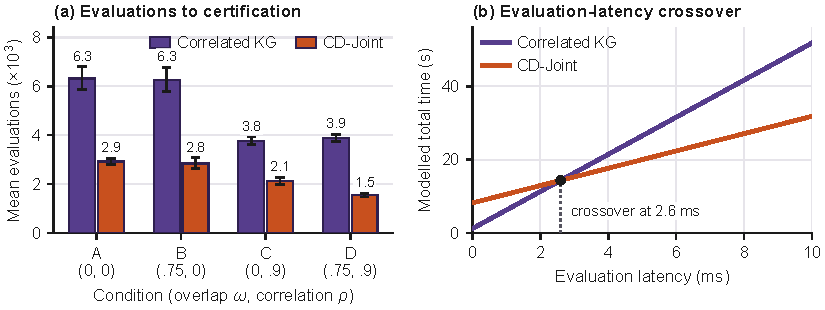
\includegraphics{figures/fig3_acquisition_and_latency.pdf}
\vspace{-12pt}
\caption{\textbf{Acquisition efficiency and evaluation-cost crossover.} \textbf{(a)} Matched Gaussian $M=64,K=8$ factorial; both policies use the same posterior and credible-ellipsoid stopping rule, with censored trials charged $12{,}000$ evaluations. Conditions A--D vary support overlap and covariance correlation; condition-level estimates appear in Table~\ref{tab:main-bed-vs-bo}, and error bars show the $95\%$ bootstrap intervals of Appendix~\ref{app:v12-bed}. \textbf{(b)} Derived cost model for the pooled cohort, $\widehat T_p(c)=\bar\tau_p(c+\bar t_{\mathrm{acq},p})$, using the \emph{reported} restricted means and per-step acquisition times (not a new wall-clock measurement). CD-Joint becomes cheaper above approximately $2.6$ ms per evaluation in this model; posterior maintenance, certificate checks and implementation overhead are omitted.}
\label{fig:main-bed-vs-bo}
\end{figure}

\subsubsection{Approximate posterior-risk acquisition and stopping diagnostics}

\paragraph{Exploratory Monte Carlo posterior-risk stopping.}
The small-graph benchmark reports two distinct stopping analyses: the shared credible ellipsoid and an additional diagnostic based on repeated posterior Monte Carlo risk estimates and per-check 99\% Clopper--Pearson intervals. The supplied experiment record does not document a simultaneous time-by-action spending schedule for the repeated checks, and selecting an action after inspecting many Monte Carlo estimates also requires selection control. Consequently the MC-risk columns are \emph{exploratory diagnostics}; ``99\% Clopper--Pearson'' means only a per-check statement, not a valid anytime stopping guarantee. These columns are not used to support the paper's formal coverage claims.

The time-and-action-uniform Monte Carlo procedure is described in Section~\ref{app:posterior-calibration}; the exploratory $M=16$ study below is not retroactively assigned that guarantee.

\begin{table}[!htbp]
\caption{\textbf{Small-problem $M=16, K=4$ approximate Bayesian root-risk VOI reference study ($40$ test seeds/condition $=1{,}120$ runs, $\varepsilon=.025, \delta=.05$, cap $1{,}000$, $0/1{,}120$ ellipsoid errors) and doubled-MC stability audit.} Reports both common $\chi^2_{15}$ ellipsoid stopping and exploratory per-check 99\% Clopper--Pearson posterior-MC risk diagnostic (not anytime calibrated). On a predetermined $40$-instance subset ($200$ states), doubling VOI MC from $(32,2048)$ to $(64,4096)$ changes ellipsoid RM by $5.49\%$ ($296.3\to 312.6$) and MC-risk RM by $9.38\%$ ($48.5\to 44.0$), leaving all policy rankings unchanged ($56.0\%$ exact / $65.0\%$ top-$2$ single-step argmax agreement).}
\label{tab:app-v12-voi16}
\uniformaligntable{0.92}{%
\begin{tabular}{@{}lrrrrrrrrr@{}}
\toprule
\textbf{Policy ($n=160$)} & \textbf{Cert.\ (\%)} & \textbf{Ellip.\ RM [95\% CI]} & \textbf{vs.\ CD} & \textbf{vs.\ KG} & \textbf{MC-risk stop$^\dagger$} & \textbf{MC-risk RM (Err)$^\dagger$} & \textbf{A / B / C / D RM} & \textbf{Acq.\ ms/st} \\
\midrule
\textsc{GP-UCB} & $96.9$ & $509.3$ [$482,537$] & $1.70\times$ & $0.93\times$ & $100.0\%$ & $53.9$ ($3/160$) & $640 / 565 / 420 / 412$ & $.024$ \\
\textsc{GP-TS} & $0.0$ & $1{,}000^*$ [$1{,}000,1{,}000$] & $3.35\times$ & $1.82\times$ & $100.0\%$ & $69.7$ ($0/160$) & $1000^* / 1000^* / 1000^* / 1000^*$ & $.050$ \\
\textsc{Noisy GP-EI} & $0.0$ & $1{,}000^*$ [$1{,}000,1{,}000$] & $3.35\times$ & $1.82\times$ & $60.0\%$ & $676.2$ ($2/160$) & $1000^* / 1000^* / 1000^* / 1000^*$ & $.166$ \\
\textsc{Correlated KG} & $92.5$ & $548.7$ [$514,583$] & $1.84\times$ & $1.00\times$ & $100.0\%$ & $53.1$ ($2/160$) & $691 / 633 / 436 / 434$ & $.082$ \\
\textsc{Correlated GP-OS} & $78.1$ & $461.3$ [$411,512$] & $1.54\times$ & $0.84\times$ & $80.6\%$ & $226.1$ ($2/160$) & $747 / \mathbf{289} / 549 / 260$ & $.093$ \\
\textsc{Bayesian VOI} & $96.3$ & $329.7$ [$299,362$] & $1.10\times$ & $0.60\times$ & $100.0\%$ & $42.3$ ($4/160$) & $428 / 356 / 293 / 241$ & $105.3$ \\
\textsc{CD-Joint} & $\mathbf{98.8}$ & $\mathbf{298.9}$ [$273,326$] & $1.00\times$ & $\mathbf{0.55\times}$ & $100.0\%$ & $\mathbf{38.9}$ ($6/160$) & $\mathbf{400} / 331 / \mathbf{255} / \mathbf{210}$ & $1.324$ \\
\bottomrule
\end{tabular}%
}
\end{table}

\subsubsection{Confirmation under anytime-valid fixed-feature stopping}

\begin{table}[!htbp]
\caption{\textbf{Confirmatory fixed-feature $M=64, K=8, d=8$ comparison pairing uniform anytime-valid Abbasi--Yadkori frequentist stopping against $\chi^2_8$ posterior credible stopping on identical instances ($100$ test seeds/condition $=4{,}800$ runs, $\varepsilon=.025, \delta=.05$, cap $12{,}000$).} On fixed non-prior $\theta^*$, $\chi^2_8$ credible stopping incurs $2.8\%$--$6.0\%$ overall false certificates (up to $12\%$ in Condition C), whereas uniform frequentist stopping incurs $0/2{,}400$ errors while preserving \textsc{CD-Joint}'s $1.65\times$ $[1.44,1.91]$ advantage over \textsc{Correlated KG}.}
\label{tab:app-v12-confirm}
\uniformaligntable{0.92}{%
\begin{tabular}{@{}llrrrrrrr@{}}
\toprule
\textbf{Stop Rule} & \textbf{Policy ($n=400$)} & \textbf{Cert.\ (\%)} & \textbf{Err.\ (/400)} & \textbf{Restr.\ Mean [95\% CI]} & \textbf{vs.\ CD [CI]} & \textbf{A / B / C / D RM} & \textbf{Acq.\ ms/st} \\
\midrule
\multirow{6}{*}{Anytime Freq.\ (AY)}
 & \textsc{GP-UCB} & $48.5$ & $0$ & $8{,}973$ [$8{,}630,9{,}305$] & $11.16\times$ $[9.05,13.9]$ & $6647 / 5380 / 11990 / 11874$ & $.017$ \\
 & \textsc{GP-TS} & $0.0$ & $0$ & $12{,}000^*$ [$12{,}000,12{,}000$] & $14.92\times$ $[12.1,18.8]$ & $12000^* / 12000^* / 12000^* / 12000^*$ & $.159$ \\
 & \textsc{Noisy GP-EI} & $0.0$ & $0$ & $12{,}000^*$ [$12{,}000,12{,}000$] & $14.92\times$ $[12.1,18.8]$ & $12000^* / 12000^* / 12000^* / 12000^*$ & $.224$ \\
 & \textsc{Correlated KG} & $\mathbf{98.2}$ & $0$ & $1{,}323$ [$1{,}138,1{,}525$] & $1.65\times$ $[1.44,1.91]$ & $544 / 411 / 2477 / 1860$ & $.222$ \\
 & \textsc{Correlated GP-OS} & $95.0$ & $0$ & $1{,}551$ [$1{,}298,1{,}819$] & $1.93\times$ $[1.59,2.38]$ & $372 / 2676 / 1670 / 1484$ & $.134$ \\
 & \textsc{CD-Joint} & $98.0$ & $\mathbf{0}$ & $\mathbf{804}$ [$640,992$] & $1.00\times$ & $\mathbf{342} / \mathbf{264} / \mathbf{1196} / \mathbf{1414}$ & $1.238$ \\
\midrule
\multirow{6}{*}{Credible ($\chi^2_8$)}
 & \textsc{GP-UCB} & $100.0$ & $24$ ($6.0\%$) & $97.0$ [$92,102$] & $1.25\times$ $[1.19,1.31]$ & $123 / 99 / 93 / 73$ & $.023$ \\
 & \textsc{GP-TS} & $99.0$ & $18$ ($4.5\%$) & $2{,}016$ [$1{,}801,2{,}244$] & $25.99\times$ $[23.1,29.1]$ & $3808 / 2113 / 1431 / 714$ & $.158$ \\
 & \textsc{Noisy GP-EI} & $10.8$ & $20$ ($5.0\%$) & $10{,}845$ [$10{,}505,11{,}157$] & $139.8\times$ $[132,148]$ & $12000^* / 12000^* / 10772 / 8606$ & $.221$ \\
 & \textsc{Correlated KG} & $100.0$ & $20$ ($5.0\%$) & $105.1$ [$99,112$] & $1.35\times$ $[1.28,1.44]$ & $126 / 98 / 113 / 84$ & $.267$ \\
 & \textsc{Correlated GP-OS} & $98.5$ & $11$ ($2.8\%$) & $305.4$ [$182,456$] & $3.94\times$ $[2.34,5.94]$ & $100 / 941 / 105 / 75$ & $.134$ \\
 & \textsc{CD-Joint} & $100.0$ & $11$ ($2.8\%$) & $\mathbf{77.6}$ [$73,82$] & $1.00\times$ & $\mathbf{100} / \mathbf{84} / \mathbf{68} / \mathbf{59}$ & $1.819$ \\
\bottomrule
\end{tabular}%
}
\end{table}

\subsection{Structural benefits of overlapping reachability}
\label{app:overlap-expanded}

\subsubsection{Support overlap under a fixed sampling policy}
\label{sec:exact-regret-experiments}
\label{sec:future-ablation}

Under matched passive \emph{TA-UCT} trajectories across $M\in\{64,256,1024\}$ ($K=M/8$ actions), $\rho\in[0,1]$, and deterministic or Bernoulli rewards ($432$ common-trace runs capped at $50{,}000$ rollouts and $1{,}536$ cold wall-clock runs capped at $1.0\text{ s}$; \cref{tab:exact-regret-overlap}), disjoint supports ($\rho=0$) yield $\tau_{\mathrm{exact}}/\tau_{\mathrm{conv}}=1.000$ identically. Once $\rho\ge 0.50$, conventional marginal stopping stalls on shared high-payoff terminals, whereas exact regret certifies from outside-support observations alone, reducing median stopping rollouts at $M=256,\rho=0.88$ to $0.049\times$ (deterministic) and $0.054\times$ (Bernoulli, an $18.4\times$ sample reduction) and cutting cold Bernoulli runtime from $>1000\text{ ms}$ ($0/8$ certified) to $114.9\text{ ms}$ ($8/8$ certified).

\begin{table}[!t]
\caption{\textbf{Passive TA-UCT exact regret versus marginal certification across support overlap $\rho$ ($432$ common traces and $1{,}536$ cold runs, $1.0\text{ s}$ cap, $g=0.42$; cold times in ms).}}
\label{tab:exact-regret-overlap}
\uniformaligntable{0.92}{%
\begin{tabular}{@{}lrrrrrr@{}}
\toprule
& & & \multicolumn{2}{c}{\textbf{Deterministic}} & \multicolumn{2}{c}{\textbf{Bernoulli}} \\
\cmidrule(lr){4-5} \cmidrule(lr){6-7}
\textbf{Regime / Size} & \textbf{$\rho$} & \textbf{Cert.\ $@\,20\text{k}$} & \textbf{$\tau_{\mathrm{ex}}/\tau_{\mathrm{cv}}$} & \textbf{Conv./Ex.\ ms} & \textbf{$\tau_{\mathrm{ex}}/\tau_{\mathrm{cv}}$} & \textbf{Conv./Ex.\ ms} \\
\midrule
Disjoint ($M{=}64$)   & $0.00$ & $1.00 / 1.00$ & $1.000$ & $76.5 / 70.8$   & $1.000$ & $120.1 / 103.2$ \\
Disjoint ($M{=}256$)  & $0.00$ & $0.96 / 0.96$ & $1.000$ & $167.5 / 183.9$ & $1.000$ & $387.3 / 355.5$ \\
Disjoint ($M{=}1024$) & $0.00$ & $0.50 / 0.50$ & $1.000$ & $561.6 / 550.2$ & $1.000$ & $1000 / 1000$   \\
\midrule
Partial ($M{=}64$)    & $0.50$ & $1.00 / 1.00$ & $0.433$ & $141.8 / \mathbf{56.2}$  & $0.369$ & $161.9 / \mathbf{66.1}$  \\
Partial ($M{=}64$)    & $0.88$ & $1.00 / 0.00$ & $0.026$ & $566.7 / \mathbf{13.1}$  & $0.014$ & $1000 / \mathbf{14.0}$   \\
Partial ($M{=}256$)   & $0.25$ & $0.50 / 0.50$ & $1.000$ & $589.9 / \mathbf{464.5}$ & $1.000$ & $1000 / 1000$            \\
Partial ($M{=}256$)   & $0.50$ & $1.00 / 0.50$ & $0.581$ & $402.9 / \mathbf{243.8}$ & $0.465$ & $574.7 / \mathbf{330.9}$ \\
Partial ($M{=}256$)   & $0.75$ & $1.00 / 0.00$ & $0.147$ & $834.7 / \mathbf{121.5}$ & $0.107$ & $1000 / \mathbf{182.5}$  \\
Partial ($M{=}256$)   & $0.88$ & $1.00 / 0.00$ & $0.049$ & $1000 / \mathbf{77.7}$   & $0.054$ & $1000 / \mathbf{114.9}$  \\
Partial ($M{=}1024$)  & $0.88$ & $0.75 / 0.00$ & $0.209$ & $1000 / \mathbf{559.7}$  & $0.247$ & $1000 / 1000$            \\
\midrule
Identical ($64\text{--}1024$) & $1.00$ & $1.00 / 0.00$ & $\mathbf{0.000}$ & $1000 / \mathbf{3.1}$ & $\mathbf{0.000}$ & $1000 / \mathbf{3.1}$ \\
\bottomrule
\end{tabular}%
}
\end{table}

\begin{figure}[t]
\centering
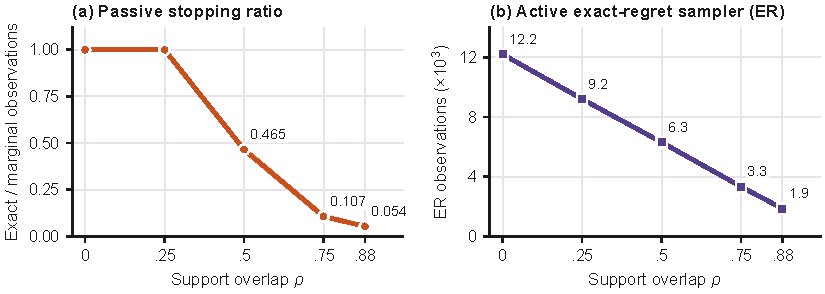
\includegraphics{figures/fig4_overlap_mechanism.pdf}
\vspace{-12pt}
\caption{\textbf{Effect of action-support overlap at $M=256$.} \textbf{(a)} Exact-versus-marginal \emph{passive} Bernoulli stopping on paired TA-UCT observations (smaller is better; the band spans the two gap settings). \textbf{(b)} Median absolute sample count, with interquartile range, for the active exact-regret sampler ER in the Hoeffding cohort; these are a different experimental condition and are not numerically interchangeable with panel (a) (Tables~\ref{tab:exact-regret-overlap}, \ref{tab:app-external-baselines}).}
\label{fig:main-overlap-mechanism}
\end{figure}
Here we isolate gains from structural overlap and test them against zero-containment natural DAGs and alternative witness-allocation policies.

\subsection{Correlated information and low-valued proxy experiments}
\label{app:bay-tables}\label{app:v8-tables}

The complete numerical comparisons preserve the separate statistical assumptions of each cohort. Every table keeps distribution-free frequentist methods, calibrated/hybrid correlated methods, and nominal surrogate tracks explicitly separated, and reports completion rates alongside capped/uncensored medians, empirical error counts (with exact Clopper--Pearson $95\%$ upper confidence bounds where relevant), recommendation regrets on capped trials, and full wall-clock compute including surrogate fitting and conic solves.

The following tables report the correlated-acquisition protocol. Bayes-IDS is a root-decision adaptation of the information-directed sampling principle \citep{russo2018ids}, not a claim that the original online-regret guarantee applies to our stopping problem. Its trial counts and evaluation budgets differ from the rectangular-confidence campaigns. Nominal linear and Gaussian-process results are conditional on their modeling assumptions; empirical error counts do not establish simultaneous coverage.

\begin{table}[!htbp]
\caption{\textbf{Off-witness proxy benchmark (50 seeds, $M=5, K=2, d=3, \varepsilon=0.015, \delta=0.05$, cap $4{,}000$).} The characteristic-time lower bound is $3.17$ pulls (rate $0.837$, optimal design weight $0.590$ on $z_{\mathrm{proxy}}$).}
\label{tab:app-e0}
\uniformaligntable{0.92}{%
\begin{tabular}{@{}lrrrrrrr@{}}
\toprule
\textbf{Method} & \textbf{Cert.\ (\%)} & \textbf{Err.} & \textbf{Median} & \textbf{IQR} & \textbf{Speedup} & \textbf{Proxy (\%)} & \textbf{Mean $z_{\mathrm{out}}$} \\
\midrule
\textsc{Exact-DAG-LUCB} & $100$ & $0$ & $791.0$ & $[691.2, 885.8]$ & $1.00\times$ & $3.3$ & $343.9$ \\
\textsc{Opt-Sep} (Indep.) & $100$ & $0$ & $791.0$ & $[691.2, 885.8]$ & $1.00\times$ & $3.3$ & $343.9$ \\
\textsc{Enclosing Box} (CD) & $46$ & $0$ & $4{,}000.0$ & $[943.2, 4{,}000.0]$ & $0.20\times$ & $74.3$ & $0.0$ \\
\textsc{GP-UCB + Joint} & $100$ & $0$ & $1{,}579.0$ & $[199.5, 2{,}010.2]$ & $0.50\times$ & $3.0$ & $54.8$ \\
\textsc{Direct-Witness + Joint} & $100$ & $0$ & $281.5$ & $[173.2, 368.2]$ & $2.81\times$ & $0.6$ & $141.6$ \\
\textsc{Bayes-IDS + Joint} & $100$ & $0$ & $37.0$ & $[28.0, 51.8]$ & $21.38\times$ & $21.0$ & $0.6$ \\
\textsc{CD-Joint} (Alg.~\ref{alg:cd-joint}) & $100$ & $0$ & $25.5$ & $[18.0, 49.0]$ & $31.02\times$ & $76.8$ & $0.0$ \\
\textsc{MaxMin-Tracking + Joint} & $100$ & $0$ & $\mathbf{15.5}$ & $[11.2, 22.0]$ & $\mathbf{51.03\times}$ & $55.2$ & $1.0$ \\
\bottomrule
\end{tabular}%
}
\end{table}

\begin{table}[!htbp]
\caption{\textbf{Full $4\times 4$ overlap $\times$ correlation phase diagram ($M=128, K=8, d=8, \varepsilon=0.03, \delta=0.05$, 20 seeds/cell, $0$ false certificates).} Entries report median evaluations to certify; bold highlights fastest method per cell.}
\label{tab:app-e1}
\uniformaligntable{0.92}{%
\begin{tabular}{@{}ccrrrrrrr@{}}
\toprule
$\omega$ & $\rho$ & \textsc{Opt-Sep} & \textsc{Box} & \textsc{GP-UCB} & \textsc{CD-Joint} & \textsc{MC-Joint} & \textsc{Track} & \textbf{CD vs.\ Opt-Sep} \\
\midrule
$0.00$ & $0.0$ & $11{,}399$ & $2{,}220$ & $1{,}538$ & $\mathbf{607.5}$ & $637.5$ & $1{,}755$ & $18.76\times$ \\
$0.00$ & $0.3$ & $11{,}092$ & $1{,}590$ & $1{,}395$ & $\mathbf{570.0}$ & $697.5$ & $1{,}815$ & $19.46\times$ \\
$0.00$ & $0.6$ & $11{,}385$ & $2{,}250$ & $1{,}358$ & $\mathbf{562.5}$ & $645.0$ & $1{,}785$ & $20.24\times$ \\
$0.00$ & $0.9$ & $11{,}908$ & $2{,}295$ & $1{,}148$ & $\mathbf{367.5}$ & $385.0$ & $945$ & $32.40\times$ \\
\midrule
$0.25$ & $0.0$ & $11{,}442$ & $3{,}615$ & $1{,}462$ & $\mathbf{510.0}$ & $532.5$ & $1{,}050$ & $22.44\times$ \\
$0.25$ & $0.3$ & $11{,}026$ & $3{,}465$ & $1{,}485$ & $\mathbf{487.5}$ & $637.5$ & $1{,}395$ & $22.62\times$ \\
$0.25$ & $0.6$ & $11{,}376$ & $3{,}210$ & $1{,}342$ & $\mathbf{442.5}$ & $622.5$ & $1{,}402$ & $25.71\times$ \\
$0.25$ & $0.9$ & $11{,}692$ & $3{,}360$ & $1{,}042$ & $\mathbf{305.0}$ & $402.5$ & $795$ & $38.34\times$ \\
\midrule
$0.50$ & $0.0$ & $11{,}345$ & $3{,}765$ & $1{,}418$ & $\mathbf{332.5}$ & $517.5$ & $622$ & $34.12\times$ \\
$0.50$ & $0.3$ & $11{,}006$ & $3{,}105$ & $1{,}358$ & $\mathbf{317.5}$ & $412.5$ & $705$ & $34.67\times$ \\
$0.50$ & $0.6$ & $11{,}586$ & $3{,}210$ & $1{,}365$ & $\mathbf{337.5}$ & $517.5$ & $840$ & $34.33\times$ \\
$0.50$ & $0.9$ & $12{,}000$ & $3{,}045$ & $1{,}200$ & $\mathbf{265.0}$ & $342.5$ & $540$ & $45.28\times$ \\
\midrule
$0.75$ & $0.0$ & $11{,}138$ & $4{,}020$ & $915$ & $\mathbf{270.0}$ & $390.0$ & $392$ & $41.25\times$ \\
$0.75$ & $0.3$ & $11{,}132$ & $3{,}090$ & $1{,}515$ & $\mathbf{240.0}$ & $377.5$ & $442$ & $46.38\times$ \\
$0.75$ & $0.6$ & $11{,}920$ & $2{,}805$ & $1{,}058$ & $\mathbf{312.5}$ & $442.5$ & $488$ & $38.15\times$ \\
$0.75$ & $0.9$ & $11{,}980$ & $3{,}225$ & $945$ & $\mathbf{245.0}$ & $317.5$ & $450$ & $48.90\times$ \\
\bottomrule
\end{tabular}%
}
\end{table}

\subsubsection{Proxy alignment, measurement cost, and matched policies}

\begin{table}[!htbp]
\caption{\textbf{Proxy alignment $\times$ relative cost sweep ($40$ paired seeds/cell, $\varepsilon=.015, \delta=.05$, $0$ errors).} Entries report median total evaluation cost for \textsc{CD-Joint (Cost-Norm)} / \textsc{CD-Joint (Uniform)} / \textsc{Direct-Witness + Joint}; cost normalization eliminates the $23\%$ penalty at weak expensive proxies ($\cos=.20, c=4$), with a small reversal relative to uniform allocation in one reported cell.}
\label{tab:app-v8-proxy}
\uniformaligntable{0.92}{%
\begin{tabular}{@{}crrrrr@{}}
\toprule
$\cos(\phi_{\mathrm{proxy}}, g^*)$ & $c=0.25$ & $c=0.50$ & $c=1.00$ & $c=2.00$ & $c=4.00$ \\
\midrule
$0.20$ & $\mathbf{172.6}$ / $199.8$ / $668.1$ & $\mathbf{225.8}$ / $241.5$ / $668.2$ & $\mathbf{325.0}$ / $325.0$ / $668.5$ & $\mathbf{468.5}$ / $491.5$ / $669.0$ & $\mathbf{667.5}$ / $824.5$ / $671.0$ \\
$0.50$ & $\mathbf{38.4}$ / $39.0$ / $637.2$ & $\mathbf{47.5}$ / $48.0$ / $637.5$ & $\mathbf{66.0}$ / $66.0$ / $638.0$ & $\mathbf{98.5}$ / $102.0$ / $639.0$ & $\mathbf{156.0}$ / $174.0$ / $641.0$ \\
$0.80$ & $\mathbf{10.6}$ / $10.8$ / $513.6$ & $\mathbf{21.0}$ / $20.8$ / $514.2$ & $\mathbf{38.0}$ / $38.0$ / $515.5$ & $\mathbf{74.0}$ / $76.0$ / $518.0$ & $\mathbf{148.0}$ / $150.0$ / $523.0$ \\
$0.95$ & $\mathbf{3.0}$ / $3.0$ / $88.1$ & $\mathbf{6.0}$ / $6.0$ / $89.8$ & $\mathbf{12.0}$ / $12.0$ / $93.0$ & $\mathbf{24.0}$ / $24.0$ / $99.5$ & $\mathbf{48.0}$ / $48.0$ / $112.5$ \\
$0.99$ & $\mathbf{2.0}$ / $2.0$ / $14.1$ & $\mathbf{4.0}$ / $4.0$ / $15.8$ & $\mathbf{8.0}$ / $8.0$ / $19.0$ & $\mathbf{16.0}$ / $16.0$ / $25.5$ & $\mathbf{32.0}$ / $32.0$ / $39.0$ \\
\bottomrule
\end{tabular}%
}
\end{table}

\begin{table}[!htbp]
\caption{\textbf{Cost-sensitive $M=5, K=2, d=3$ low-valued proxy benchmark ($80$ paired seeds/cell $\times 6$ cells $\times 7$ policies $\times 2$ stopping rules $=6{,}720$ runs, $\varepsilon=.015, \delta=.05$, cap $1{,}500$, $0/6{,}720$ errors).} Entries report restricted mean total certification cost (\emph{proxy-arm query \%}). Top block uses the exact $\chi^2_3$ posterior credible ellipsoid; bottom block uses the uniform anytime-valid Abbasi--Yadkori frequentist ellipsoid.}
\label{tab:app-v12-proxy5}
\uniformaligntable{0.92}{%
\begin{tabular}{@{}lcrrrrrrr@{}}
\toprule
\textbf{Stop Rule} & $(\cos, c_{\rm proxy})$ & \textbf{GP-UCB} & \textbf{GP-TS} & \textbf{GP-EI} & \textbf{GP-OS} & \textbf{Correlated KG} & \textbf{Bayesian VOI} & \textbf{CD-Joint} \\
\midrule
\multirow{6}{*}{Credible ($\chi^2_3$)}
 & $(.50, 0.25)$ & $111.2$ ($0\%$) & $128.8$ ($2\%$) & $1030$ ($9\%$) & $91.4$ ($0\%$) & $7.8$ ($54\%$) & $8.9$ ($64\%$) & $\mathbf{6.9}$ ($72\%$) \\
 & $(.50, 1.00)$ & $111.2$ ($0\%$) & $129.2$ ($2\%$) & $1348$ ($0\%$) & $91.4$ ($0\%$) & $13.8$ ($49\%$) & $14.7$ ($48\%$) & $\mathbf{12.5}$ ($58\%$) \\
 & $(.50, 4.00)$ & $111.2$ ($0\%$) & $131.1$ ($2\%$) & $1348$ ($0\%$) & $91.4$ ($0\%$) & $33.3$ ($48\%$) & $34.2$ ($28\%$) & $\mathbf{31.1}$ ($43\%$) \\
 & $(.95, 0.25)$ & $12.1$ ($26\%$) & $60.6$ ($29\%$) & $\mathbf{0.7}$ ($100\%$) & $90.7$ ($0\%$) & $1.8$ ($71\%$) & $1.5$ ($78\%$) & $\mathbf{0.7}$ ($100\%$) \\
 & $(.95, 1.00)$ & $13.5$ ($26\%$) & $61.6$ ($29\%$) & $1008$ ($0\%$) & $90.7$ ($0\%$) & $4.0$ ($54\%$) & $3.6$ ($70\%$) & $\mathbf{2.7}$ ($100\%$) \\
 & $(.95, 4.00)$ & $18.9$ ($26\%$) & $65.5$ ($29\%$) & $1240$ ($0\%$) & $90.7$ ($0\%$) & $\mathbf{10.6}$ ($50\%$) & $10.8$ ($53\%$) & $10.9$ ($100\%$) \\
\midrule
\multirow{6}{*}{Anytime Freq.}
 & $(.50, 0.25)$ & $1500^*$ ($0\%$) & $1500^*$ ($0\%$) & $1499^*$ ($0\%$) & $683.2$ ($0\%$) & $99.0$ ($27\%$) & $40.9$ ($68\%$) & $\mathbf{37.5}$ ($71\%$) \\
 & $(.50, 1.00)$ & $1500^*$ ($0\%$) & $1500^*$ ($0\%$) & $1477^*$ ($0\%$) & $683.2$ ($0\%$) & $124.4$ ($26\%$) & $73.1$ ($53\%$) & $\mathbf{68.7}$ ($55\%$) \\
 & $(.50, 4.00)$ & $1500^*$ ($0\%$) & $1502^*$ ($0\%$) & $1477^*$ ($0\%$) & $683.2$ ($0\%$) & $222.5$ ($26\%$) & $170.4$ ($35\%$) & $\mathbf{162.4}$ ($38\%$) \\
 & $(.95, 0.25)$ & $349.5$ ($11\%$) & $1220^*$ ($12\%$) & $\mathbf{3.1}$ ($100\%$) & $668.2$ ($0\%$) & $24.6$ ($32\%$) & $34.2^\dagger$ ($65\%$) & $\mathbf{3.1}$ ($100\%$) \\
 & $(.95, 1.00)$ & $355.7$ ($11\%$) & $1224^*$ ($12\%$) & $1464^*$ ($0\%$) & $668.2$ ($0\%$) & $31.9$ ($32\%$) & $102.0^\dagger$ ($60\%$) & $\mathbf{12.3}$ ($100\%$) \\
 & $(.95, 4.00)$ & $380.6$ ($11\%$) & $1237^*$ ($12\%$) & $1489^*$ ($0\%$) & $668.2$ ($0\%$) & $60.2$ ($31\%$) & $89.5^\dagger$ ($57\%$) & $\mathbf{49.3}$ ($100\%$) \\
\bottomrule
\multicolumn{9}{@{}l@{}}{\scriptsize $^\dagger$Under long-horizon frequentist stopping at $\cos=.95$, \textsc{Bayesian VOI} median costs are $7.0/16.5/46.0$, but $1$--$4$ capped outliers ($95\%$--$98.8\%$ cert.) inflate its mean once MC risk saturates at $0$.}
\end{tabular}%
}
\end{table}

\subsubsection{Independent effects of overlap and correlation}

\begin{table}[!htbp]
\caption{\textbf{Deconfounded $4\times4\times3$ full-rank ($M=64, K=8$) overlap $\times$ correlation $\times$ mismatch factorial ($16$ paired seeds/cell, $\varepsilon=.025, \delta=.05$, cap $12{,}000$).} At $\rho=0$, $K(0)=\tau_0^2 I_{64}$ is strictly diagonal and \textsc{Corr-GP OS} equals \textsc{Diag-GP OS} identically. Top block reports marginal medians by mismatch $\xi$; bottom block reports selected $(\omega,\rho)$ slices at $\xi=0$.}
\label{tab:app-v8-phase}
\uniformaligntable{0.92}{%
\begin{tabular}{@{}lrrrrrr@{}}
\toprule
\textbf{Slice ($n$ runs/method)} & \textbf{Indep.\ OS} & \textbf{Diag-GP OS} & \textbf{Corr-GP UCB} & \textbf{Corr-GP OS} & \textbf{Corr-GP CD} & \textbf{Smart Hybrid} \\
\midrule
All $(\omega,\rho)$, $\xi=.000$ ($256$) & $6{,}232$ ($100\%$) & $1{,}650$ ($95.7\%$) & $2{,}610$ ($100\%$) & $1{,}485$ ($96.9\%$) & $\mathbf{1{,}380}$ ($100\%$) & $1{,}410$ ($100\%$) \\
All $(\omega,\rho)$, $\xi=.015$ ($256$) & $6{,}979$ ($100\%$) & $2{,}055$ ($91.8\%$) & $3{,}240$ ($100\%$) & $1{,}995$ ($87.9\%$) & $\mathbf{1{,}770}$ ($100\%$) & $7{,}561$ ($100\%$) \\
All $(\omega,\rho)$, $\xi=.045$ ($256$) & $6{,}516$ ($99.6\%$) & $2{,}370$ ($84.0\%$) & $2{,}820$ ($100\%$) & $2{,}370$ ($77.0\%$) & $\mathbf{1{,}755}$ ($100\%$) & $7{,}104$ ($99.2\%$) \\
\midrule
$\xi=0$, $\omega=.00, \rho=.0$ (diag.\ $K$) & $7{,}715$ & $2{,}505$ & $3{,}735$ & $2{,}505$ & $\mathbf{1{,}950}$ & $2{,}130$ \\
$\xi=0$, $\omega=.00, \rho=.9$ (corr.\ only) & $6{,}165$ & $2{,}970$ & $1{,}995$ & $2{,}100$ & $\mathbf{1{,}275}$ & $1{,}290$ \\
$\xi=0$, $\omega=.75, \rho=.0$ (overlap only) & $6{,}599$ & $1{,}448$ & $3{,}330$ & $1{,}448$ & $\mathbf{1{,}373}$ & $1{,}403$ \\
$\xi=0$, $\omega=.75, \rho=.9$ (both) & $5{,}817$ & $1{,}193$ & $2{,}280$ & $1{,}050$ & $\mathbf{1{,}005}$ & $1{,}035$ \\
\bottomrule
\end{tabular}%
}
\end{table}

\begin{figure}[t]
\centering
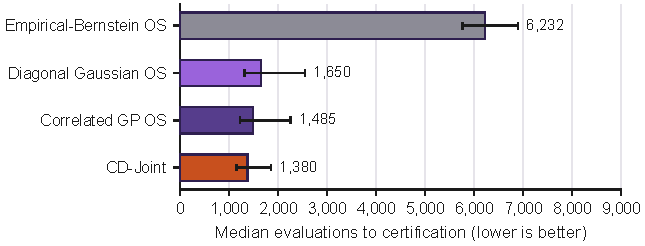
\includegraphics{figures/fig5_correlation_factorial.pdf}
\vspace{-12pt}
\caption{\textbf{Comparison of correlation models and acquisition policies.} Controlled $M=64$, $K=8$, $\xi=0$ zero-containment factorial medians from Table~\ref{tab:app-v8-phase}, with interquartile ranges over the $256$ pooled runs. The differences between bounded empirical-Bernstein inference, diagonal Gaussian inference, correlated-GP inference, and CD-Joint are \emph{mechanistic ablations with different model assumptions}; only the final correlated comparison isolates acquisition after the common correlated model.}
\label{fig:main-correlation-factorial}
\end{figure}

\subsection{Independent-observation baselines and witness ablations}
\label{app:v3-strengthening}

\subsubsection{Decision-aware acquisition implementation and confidence-box controls}
\label{sec:strengthening-experiments}

To operationalize \cref{thm:adaptive-oracle-coupling} with an adaptive controller, \emph{Charged Dual Covers}, \emph{Direct-Graph-Regret}, and \emph{Factorized-Regret} break all upper-bound ties deterministically by $(u_t(z),-z)$ over canonical terminal IDs so every exact-regret representation returns the identical quadruple $(a_t,\mathcal R_t(a_t),p_t,q_t)$. Prior to stopping at $\mathcal R_t(a_t)\le\varepsilon$, \emph{Exact-Regret-DAG-LUCB} traverses a precomputed shortest DAG path to whichever of $\{p_t,q_t\}$ has the wider current interval, whereas \emph{Marginal-DAG-LUCB} compares the lower-bound leader $\hat a_t$ against $\tilde b_t=\arg\max_{b\ne \hat a_t}U_t(b)$ and queries the wider optimistic witness across $S(\hat a_t)$ and $S(\tilde b_t)$. An automated $9{,}029$-step audit across seven synthetic and SameGame DAGs confirmed zero path, reward, witness, or stopping discrepancies across all three exact-regret representations (\cref{tab:app-active-lucb}).

\begin{table}[!t]
\caption{\textbf{Hoeffding versus predictable Empirical Bernstein (EB) boxes under marginal and exact certification ($82$ common traces and $408$ cold runs, $1.0\text{ s}$ cap, $0$ false certificates; times in ms).}}
\label{tab:app-emp-bernstein-lucb}
\uniformaligntable{0.92}{%
\begin{tabular}{@{}lrrrrr@{}}
\toprule
\textbf{Cohort (Instances)} & \textbf{Hoeff.\ Conv.} & \textbf{Hoeff.\ Exact} & \textbf{EB Conv.} & \textbf{EB Exact} & \textbf{Med.\ $\tau_{\mathrm{EB,ex}}$} \\
\midrule
SameGame $5\times 5\ d{=}3$ ($6$)     & $784.1\ (33\%)$ & $718.9\ (33\%)$ & $881.8\ (33\%)$ & $757.8\ (33\%)$ & $24{,}000^*$ \\
SameGame $6\times 6\ d{=}3$ ($6$)     & $1000\ (0\%)$   & $1000\ (0\%)$   & $1000\ (17\%)$  & $\mathbf{997.3}\ (\mathbf{33\%})$ & $24{,}000^*$ \\
Std.\ $15\times 15$ Endg.\ $d{=}3$ ($20$) & $1000\ (15\%)$ & $922.3\ (60\%)$ & $73.1\ (100\%)$ & $\mathbf{25.9}\ (\mathbf{100\%})$ & $\mathbf{768}$ \\
Std.\ $15\times 15$ Endg.\ $d{=}4$ ($20$) & $1000\ (35\%)$ & $142.0\ (65\%)$ & $131.2\ (85\%)$ & $\mathbf{3.35}\ (\mathbf{100\%})$ & $\mathbf{94}$  \\
Overlap $256,\rho{=}0.00$ ($6$, Ber.) & $435.5\ (100\%)$& $\mathbf{416.5}\ (\mathbf{100\%})$ & $741.2\ (0\%)$ & $695.2\ (0\%)$ & $50{,}000^*$ \\
Overlap $256,\rho{=}0.75$ ($6$, Ber.) & $869.0\ (0\%)$  & $\mathbf{241.4}\ (\mathbf{100\%})$ & $925.3\ (0\%)$ & $256.8\ (100\%)$ & $6{,}506$ \\
Overlap $256,\rho{=}0.88$ ($6$, Ber.) & $841.6\ (0\%)$  & $152.7\ (100\%)$ & $895.1\ (0\%)$ & $\mathbf{148.0}\ (\mathbf{100\%})$ & $\mathbf{2{,}868}$ \\
\bottomrule
\end{tabular}%
}
\end{table}

\begin{table}[!t]
\caption{\textbf{Active witness allocation (\emph{Exact-Regret-DAG-LUCB}) versus \emph{Marginal-DAG-LUCB} and passive TA-UCT ($912$ cold runs, $1.0\text{ s}$ cap, $0$ false certificates; median runtime in ms).}}
\label{tab:app-active-lucb}
\uniformaligntable{0.92}{%
\begin{tabular}{@{}lrrrrr@{}}
\toprule
\textbf{Benchmark} & \textbf{TA-UCT + Ex.} & \textbf{Marg.\ LUCB} & \textbf{Exact LUCB (Dual)} & \textbf{Exact LUCB (Dir.)} & \textbf{Steps} \\
\midrule
Overlap $M{=}64,\rho{=}0.75$  & $32.3$  & $145.3$ & $\mathbf{9.8}$   & $28.4$  & $884$ \\
Overlap $M{=}256,\rho{=}0.25$ & $783^*$ & $662.1$ & $\mathbf{304.7}$ & $868.6$ & $9{,}158$ \\
Overlap $M{=}256,\rho{=}0.50$ & $479.2$ & $1000^*$ & $\mathbf{210.2}$ & $597.8$ & $6{,}285$ \\
Overlap $M{=}256,\rho{=}0.75$ & $242.3$ & $1000^*$ & $\mathbf{114.4}$ & $347.3$ & $3{,}344$ \\
Overlap $M{=}256,\rho{=}0.88$ & $156.4$ & $1000^*$ & $\mathbf{56.1}$  & $205.7$ & $1{,}859$ \\
Parity Grid ($r=16$)          & $\mathbf{97.8}$ & $893.1$ & $465.4$ & $1000^*$ & $6{,}195$ \\
Std.\ $15\times 15\ d{=}3$ (EB) & $34.5$ & $49.4$ & $\mathbf{24.2}$ & $43.5$ & $1{,}028$ \\
\bottomrule
\end{tabular}%
}
\end{table}

\subsubsection{Structured pure-exploration baselines and $2\times 2$ controls}
\label{sec:external-baselines-experiments}

To separate stopping-rule improvements from active sampling improvements, we evaluate \emph{Exact-Regret-DAG-LUCB} against three structured pure-exploration baselines under matched $(\varepsilon,\delta=0.05)$, identical terminal reward tapes, and identical nested confidence boxes ($936$ counterbalanced timed runs and $117$ isolated memory runs, $0$ false certificates):
\begin{enumerate}[leftmargin=18pt, itemsep=2pt]
\item \textbf{\emph{LUCB-micro}}~\citep{huang}: Identifies the empirical macro-action leader $B_t=\arg\max_{a\in\mathcal A}\max_{z\in S(a)}\hat\mu_t(z)$ and optimistic marginal challenger $C_t=\arg\max_{b\ne B_t}U_t(b)$, querying the wider optimistic micro-terminal between $\arg\max_{z\in S(B_t)}u_t(z)$ and $\arg\max_{z\in S(C_t)}u_t(z)$.
\item \textbf{\emph{UGapE-DAG}}~\citep{gabillon2012best,kaufmann}: Specializes root best-action UGapE to transposition-pooled DAGs (alongside a tree-unrolled control \emph{UGapE-Tree}), selecting $B_t=\arg\min_{a\in\mathcal A}(\max_{b\ne a}U_t(b)-L_t(a))$, challenger $C_t=\arg\max_{b\ne B_t}U_t(b)$, and descending optimistically from the wider of $\{B_t,C_t\}$.
\item \textbf{\emph{VarDE-Exact}} (variance-decrement witness allocation inspired by~\citealp{luong2026varde}): Replaces raw interval width when choosing between leader and challenger witnesses with the expected one-step confidence-width decrement score $\sqrt{\hat\sigma_{z,t}^2/(n_z(t)(n_z(t)+1))}$, evaluated under both marginal witnesses (\emph{VarDE-Marg}) and exact shared-support witnesses (\emph{VarDE-Exact}).
\end{enumerate}
In a $2\times 2$ \texttt{(Sampler $\times$ Certificate)} factorial, both \emph{LUCB-micro} and \emph{UGapE-DAG} are run under their native marginal stopping rule ($\Delta_t\le\varepsilon$) and under our exact shared-support stopping rule ($\min_a\mathcal R_t(a)\le\varepsilon$). \cref{tab:app-external-baselines} reports the full breakdown across $M\in\{64,256\}$, $\rho\in[0,0.88]$, Hoeffding and Empirical Bernstein boxes, and zero-containment contiguous windows (isolated memory is $247$--$258\text{ KiB}$ at $M=64$ and $985$--$1{,}132\text{ KiB}$ at $M=256$).

\begin{table}[!t]
\caption{\textbf{Extended $2\times 2$ \texttt{(Sampler $\times$ Certificate)} comparison against structured pure-exploration baselines ($936$ timed runs, $1.0\text{ s} / 36{,}000$-step cap, $0$ false certificates; median time in ms, $^*$capped).}}
\label{tab:app-external-baselines}
\uniformaligntable{0.92}{%
\begin{tabular}{@{}llrrrrr@{}}
\toprule
\textbf{Family / Box} & \textbf{$\rho$} & \textbf{LUCB-m (Mg/Ex)} & \textbf{UGapE (Mg/Ex)} & \textbf{VarDE-Ex.} & \textbf{Exact LUCB} & \textbf{Steps} \\
\midrule
Overlap $64$ (Hoeff.)  & $0.00$ & $27.7 / 52.4$   & $27.2 / 53.8$   & $\mathbf{24.0}$ & $28.8$ & $2{,}543$ \\
Overlap $64$ (Hoeff.)  & $0.25$ & $61.9 / 91.1$   & $53.4 / 88.8$   & $\mathbf{21.9}$ & $24.5$ & $2{,}015$ \\
Overlap $64$ (Hoeff.)  & $0.50$ & $107.2 / 153.4$ & $89.8 / 144.8$  & $17.4$          & $\mathbf{17.1}$ & $1{,}419$ \\
Overlap $64$ (Hoeff.)  & $0.75$ & $154.6 / 215.0$ & $126.4 / 197.2$ & $\mathbf{10.2}$ & $10.8$ & $893$   \\
Overlap $64$ (Hoeff.)  & $0.88$ & $164.8 / 245.4$ & $140.7 / 219.1$ & $7.2$           & $\mathbf{6.8}$  & $618$   \\
\midrule
Overlap $256$ (Hoeff.) & $0.00$ & $\mathbf{182.3} / 390.3$ & $239.6 / 460.7$ & $257.4$ & $334.2$ & $12{,}201$ \\
Overlap $256$ (Hoeff.) & $0.25$ & $645.5 / 820.8$ & $450.0 / 642.0$ & $\mathbf{238.0}$ & $296.9$ & $9{,}201$ \\
Overlap $256$ (Hoeff.) & $0.50$ & $1000^* / 1000^*$ & $717.4 / 984^*$ & $\mathbf{205.0}$ & $226.5$ & $6{,}304$ \\
Overlap $256$ (Hoeff.) & $0.75$ & $1000^* / 1000^*$ & $869^* / 1000^*$ & $\mathbf{92.8}$  & $109.9$ & $3{,}328$ \\
Overlap $256$ (Hoeff.) & $0.88$ & $1000^* / 1000^*$ & $871^* / 1000^*$ & $\mathbf{57.9}$  & $61.5$  & $1{,}862$ \\
\midrule
Overlap $256$ (EB)     & $0.50$ & $1000^* / 1000^*$ & $1000^* / 1000^*$ & $\mathbf{143.7}$ & $157.4$ & $5{,}097$ \\
Overlap $256$ (EB)     & $0.75$ & $1000^* / 1000^*$ & $1000^* / 1000^*$ & $79.5$           & $\mathbf{76.3}$ & $2{,}754$ \\
Overlap $256$ (EB)     & $0.88$ & $1000^* / 1000^*$ & $1000^* / 1000^*$ & $46.2$           & $\mathbf{44.2}$ & $1{,}611$ \\
Window $256$ (Hoeff.)  & $0.50$ & $507.9 / 687.1$   & $845.4 / 1000^*$  & $\mathbf{85.7}$  & $108.4$ & $8{,}582$ \\
\bottomrule
\end{tabular}%
}
\end{table}

\begin{figure}[!htbp]
\centering
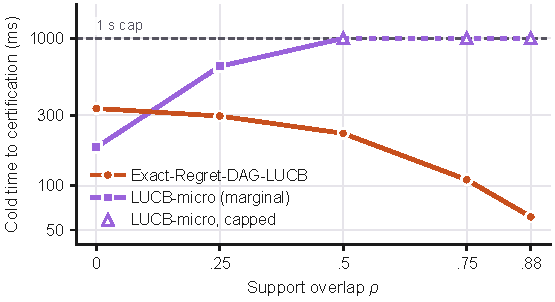
\includegraphics{figures/fig6_overlap_crossover.pdf}
\vspace{-12pt}
\caption{\textbf{The overlap crossover.} Recorded medians for the $M=256$ Hoeffding cohort. Hollow triangles identify baseline cohorts with capped runs, rather than completed $1000$-ms certification times. Table~\ref{tab:app-external-baselines} compares all samplers and stopping rules.}
\label{fig:statistical-performance}
\end{figure}

\subsubsection{Inside-witness allocation and safeguards}

\begin{figure}[t]
\centering
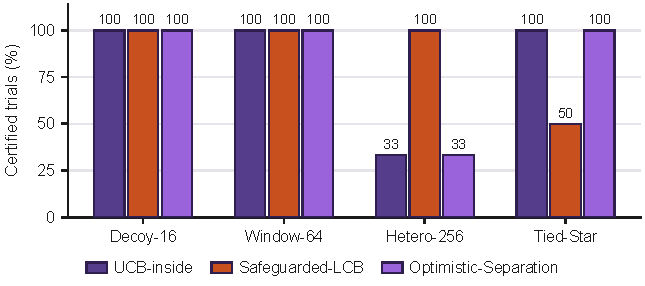
\includegraphics{figures/fig7_inside_witness.pdf}
\vspace{-12pt}
\caption{\textbf{Inside-witness robustness.} Certification rates reported in Tables~\ref{tab:app-hybrid-and-star} and~\ref{tab:app-star-eps}. The first three tasks use the synthetic diagnostic budgets; TiedStar uses exact $\varepsilon=0$ and its separate $50{,}000$-observation cap. The safeguard resolves the broad-support and decoy regimes but is not uniformly best on exact tied-star certification.}
\label{fig:inside-witness}
\end{figure}

Holding outside-witness selection $q_t=\arg\max_{z\notin S(a_t)}(u_t(z),-z)$ and exact stopping fixed, we first compare inside witnesses chosen by upper bound (\texttt{ucb}), empirical mean (\texttt{mean}), and scanned lower bound (\texttt{lcb}) across $456$ runs ($1.0\text{ s}$ and $30{,}000$-step cap; \cref{tab:app-inside-ablation}). We then evaluate \texttt{DualWitnessCovers} with charged subscription updates—which stores $(l_t(d),u_t(z^*(d)),-z^*(d))$ alongside $(u_t(d),-z^+(d))$ at each segment-tree node—paired with \emph{LCB-fast}, our parameter-free \emph{Safeguarded-LCB} rule (\cref{prop:active-hybrid}), and \emph{Optimistic-Separation} (\cref{thm:active-os}) across $768$ synthetic and mid-game SameGame runs (\cref{tab:app-hybrid-and-star}) and $160$ runs on the non-containment tied-star family ($N=8$, $\Gamma=0.25$, $\varepsilon\downarrow 0$; \cref{tab:app-star-eps}).

\begin{table}[!t]
\caption{\textbf{Inside-witness selection ablation inside \emph{Exact-Regret-DAG-LUCB} ($456$ timed runs, $1.0\text{ s} / 30{,}000$-step cap, $0$ false certificates; median runtime in ms).}}
\label{tab:app-inside-ablation}
\uniformaligntable{0.92}{%
\begin{tabular}{@{}lrrrrrr@{}}
\toprule
\textbf{Benchmark Family} & \textbf{UCB Cert.} & \textbf{UCB ms} & \textbf{Mean Cert.} & \textbf{Mean ms} & \textbf{LCB Cert.} & \textbf{LCB ms} \\
\midrule
Decoy Trap ($M{=}16$)        & $\mathbf{100\%}$ & $\mathbf{34.5}$  & $66.7\%$ & $41.9$  & $66.7\%$ & $40.5$ \\
Contig.\ Window ($M{=}64$)   & $\mathbf{100\%}$ & $\mathbf{20.8}$  & $\mathbf{100\%}$ & $32.0$ & $91.7\%$ & $30.3$ \\
Contig.\ Window ($M{=}256$)  & $\mathbf{100\%}$ & $\mathbf{102.6}$ & $\mathbf{100\%}$ & $257.5$& $\mathbf{100\%}$ & $233.7$ \\
Overlap $256,\rho{=}0.75$    & $\mathbf{100\%}$ & $\mathbf{110.7}$ & $\mathbf{100\%}$ & $178.0$& $\mathbf{100\%}$ & $171.3$ \\
Hetero Support ($M{=}64$)    & $\mathbf{100\%}$ & $\mathbf{154.9}$ & $\mathbf{100\%}$ & $189.6$& $\mathbf{100\%}$ & $182.7$ \\
Hetero Support ($M{=}256$)   & $33.3\%$         & $\mathbf{534.8}$ & $\mathbf{100\%}$ & $896.4$& $\mathbf{100\%}$ & $853.0$ \\
SG $15{\times}15$ Mid ($0$-c.) & $30.0\%$       & $923.6$          & $50.0\%$ & $934.7$& $\mathbf{55.0\%}$ & $\mathbf{889.0}$ \\
\bottomrule
\end{tabular}%
}
\end{table}

\begin{table}[!t]
\caption{\textbf{\texttt{DualWitnessCovers} with charged subscription updates safeguarded hybrid evaluation ($768$ runs across $1.0\text{ s}$ synthetic cohorts and the full $20$-board $1.8\text{ s}$ mid-game SameGame cohort; certification rate and median/mean ms).}}
\label{tab:app-hybrid-and-star}
\uniformaligntable{0.92}{%
\begin{tabular}{@{}lrrrr@{}}
\toprule
\textbf{Benchmark Cohort} & \textbf{UCB-inside} & \textbf{LCB-fast} & \textbf{Safeguarded-LCB} & \textbf{Opt.-Sep.} \\
\midrule
Decoy Trap ($M{=}16$)             & $\mathbf{100\%}\ (39.8)$  & $66.7\%\ (38.2)$          & $\mathbf{100\%}\ (41.3)$  & $\mathbf{100\%}\ (46.2)$ \\
Contig.\ Window ($M{=}64$)        & $\mathbf{100\%}\ (24.3)$  & $91.7\%\ (24.2)$          & $\mathbf{100\%}\ (25.3)$  & $\mathbf{100\%}\ (24.2)$ \\
Contig.\ Window ($M{=}256$)       & $\mathbf{100\%}\ (129.9)$ & $\mathbf{100\%}\ (\mathbf{127.5})$ & $\mathbf{100\%}\ (130.2)$ & $\mathbf{100\%}\ (136.0)$ \\
Overlap $256,\rho{=}0.75$         & $\mathbf{100\%}\ (122.7)$ & $\mathbf{100\%}\ (115.3)$ & $\mathbf{100\%}\ (116.9)$ & $\mathbf{100\%}\ (\mathbf{112.3})$ \\
Hetero Support ($M{=}64$)         & $\mathbf{100\%}\ (174.8)$ & $\mathbf{100\%}\ (\mathbf{154.6})$ & $\mathbf{100\%}\ (158.8)$ & $\mathbf{100\%}\ (198.3)$ \\
Hetero Support ($M{=}256$)        & $33.3\%\ (596.7)$         & $\mathbf{100\%}\ (\mathbf{549.1})$ & $\mathbf{100\%}\ (572.0)$ & $33.3\%\ (683.6)$ \\
SG Midg.\ ($10$ bds, $1.0\text{ s}$) & $30.0\%\ (1000^*)$     & $\mathbf{55.0\%}\ (\mathbf{806.1})$ & $50.0\%\ (909.7)$        & $30.0\%\ (1000^*)$ \\
SG Midg.\ ($19$ $0$-c., $1.8\text{ s}$)& $36.8\%\ (1412)$     & $\mathbf{47.4\%}\ (\mathbf{1239})$  & $42.1\%\ (1335)$         & $36.8\%\ (1435)$ \\
SG Midg.\ ($1$ w/ cont., $1.8\text{ s}$)& $\mathbf{100\%}\ (0.56)$ & $\mathbf{100\%}\ (\mathbf{0.54})$ & $\mathbf{100\%}\ (0.55)$ & $\mathbf{100\%}\ (0.62)$ \\
\bottomrule
\end{tabular}%
}
\end{table}

\begin{table}[!t]
\caption{\textbf{Non-containment tied-star Bernoulli family ($N{=}8,\Gamma{=}0.25$, $160$ runs, $50{,}000$-step cap; certification rate and median observation steps as $\varepsilon\downarrow 0$).}}
\label{tab:app-star-eps}
\uniformaligntable{0.92}{%
\begin{tabular}{@{}lrrrr@{}}
\toprule
\textbf{Tolerance $\varepsilon$} & \textbf{UCB-inside} & \textbf{Safeguarded} & \textbf{Opt.-Sep} & \textbf{LUCB-micro} \\
\midrule
$\varepsilon = 0.10$        & $\mathbf{100\%}\ (2{,}636)$ & $\mathbf{100\%}\ (4{,}511)$ & $\mathbf{100\%}\ (\mathbf{2{,}038})$ & $\mathbf{100\%}\ (8{,}153)$ \\
$\varepsilon = 0.05$        & $\mathbf{100\%}\ (3{,}561)$ & $75.0\%\ (21{,}791)$        & $\mathbf{100\%}\ (\mathbf{3{,}233})$ & $\mathbf{100\%}\ (38{,}720)$ \\
$\varepsilon = 0.02$        & $\mathbf{100\%}\ (4{,}357)$ & $50.0\%\ (27{,}709)$        & $\mathbf{100\%}\ (\mathbf{4{,}057})$ & $0.0\%\ (50{,}000^*)$ \\
$\varepsilon = 0.01$        & $\mathbf{100\%}\ (4{,}753)$ & $50.0\%\ (27{,}886)$        & $\mathbf{100\%}\ (\mathbf{4{,}539})$ & $0.0\%\ (50{,}000^*)$ \\
$\varepsilon = 0.00$ (exact)& $\mathbf{100\%}\ (5{,}031)$ & $50.0\%\ (28{,}171)$        & $\mathbf{100\%}\ (\mathbf{4{,}846})$ & $0.0\%\ (50{,}000^*)$ \\
\bottomrule
\end{tabular}%
}
\end{table}

\begin{table}[!htbp]
\caption{\textbf{Hard-regime adaptive exact-regret sampling across $19$ zero-containment mid-game $15\times 15$ SameGame boards ($3$ paired seeds $=57$ runs/method, $1.8$ s / $60$k cap), Tied-Star ($\varepsilon\in\{0,.01,.02,.05\}$, $16$ seeds), Decoy-16, and Hetero-256 ($16$ seeds, Empirical Bernstein $\delta=.05$, $0$ errors).}}
\label{tab:app-v8-samegame}
\uniformaligntable{0.92}{%
\begin{tabular}{@{}lrrrrrrr@{}}
\toprule
\textbf{Method} & \textbf{SG-19ZC (\%)} & \textbf{SG-All20 (\%)} & \textbf{Star $\varepsilon=0$} & \textbf{Star $\varepsilon=.01$} & \textbf{Star $\varepsilon=.05$} & \textbf{Decoy-16} & \textbf{Hetero-256} \\
\midrule
\textsc{Exact-Regret-DAG-LUCB} & $24.6$ & $28.3$ & $3{,}595$ ($93.8\%$) & $3{,}135$ ($93.8\%$) & $2{,}413$ ($100\%$) & $475$ & $9{,}015$ \\
\textsc{LCB-fast} & $\mathbf{36.8}$ & $\mathbf{40.0}$ & $4{,}013$ ($62.5\%$) & $3{,}628$ ($62.5\%$) & $2{,}475$ ($81.3\%$) & $443^\ddagger$ & $5{,}220$ \\
\textsc{Safeguarded-LCB} & $31.6$ & $35.0$ & $4{,}041$ ($62.5\%$) & $3{,}654$ ($62.5\%$) & $2{,}489$ ($81.3\%$) & $443$ & $5{,}220$ \\
\textsc{Optimistic-Separation} & $22.8$ & $26.7$ & $3{,}232$ ($100\%$) & $2{,}921$ ($100\%$) & $2{,}070$ ($100\%$) & $475$ & $9{,}004$ \\
\textsc{VarDE-Exact} & $24.6$ & $28.3$ & $3{,}610$ ($93.8\%$) & $3{,}235$ ($93.8\%$) & $2{,}370$ ($100\%$) & $471$ & $8{,}255$ \\
\textsc{Adaptive-OS-LCB} & $22.8$ & $26.7$ & $\mathbf{2{,}920}$ ($\mathbf{100\%}$) & $\mathbf{2{,}630}$ ($\mathbf{100\%}$) & $\mathbf{1{,}896}$ ($\mathbf{100\%}$) & $396$ & $5{,}220$ \\
\textsc{KL-Info-Hybrid} & $22.8$ & $26.7$ & $3{,}140$ ($\mathbf{100\%}$) & $2{,}761$ ($\mathbf{100\%}$) & $2{,}016$ ($\mathbf{100\%}$) & $\mathbf{356}$ & $\mathbf{5{,}034}$ \\
\bottomrule
\multicolumn{8}{@{}l@{}}{\scriptsize $^\ddagger$On Decoy-16, \textsc{LCB-fast} suffers decoy-trapping mean inflation ($803.4$ mean, Q75 $1{,}330$), whereas \textsc{KL-Info-Hybrid} achieves $369.4$ mean.}
\end{tabular}%
}
\end{table}

\subsection{Containment controls on natural and routing DAGs}

To test whether shared-support certification depends on trivial support inclusions ($S(b)\subseteq S(a)$), we evaluate $58$ natural SameGame and routing DAGs across $812$ counterbalanced timed runs and $133$ isolated memory runs under Empirical Bernstein boxes ($1.8\text{ s}$ and $60{,}000$-step cap, $0$ false certificates; \cref{tab:app-zero-containment-inside}), backed by a compiled \texttt{-O3} C++17 SameGame playout engine verified against exact dynamic-programming playout expectations. Four cohorts are stratified by support containment: (i)~the $20$ standard $15\times 15$ depth-$4$ SameGame endgames ($\varepsilon=0.04$), split into the $13$ containment-present boards versus the $7$ strictly zero-containment boards; (ii)~the $20$ standard $15\times 15$ mid-game boards ($\sim 62$ remaining tiles, $d=4$, $\varepsilon=0.025$), where $19/20$ boards have strictly zero root-support containments ($277$ median / $736$ max vertices, $87.6\%$ leaf transposition rate); (iii)~all $6$ dense random $6\times 6$ depth-$4$ boards ($0/6$ containments, $517$ median / $1{,}099$ max vertices, $\varepsilon=0.05$); and (iv)~$12$ five-layer stochastic routing DAGs ($W\in\{32,96\}$, $|V|\in\{313,889\}$, $0/12$ containments, $95.0\%$ transposition rate, $\varepsilon=0.06$).

\begin{table}[!t]
\caption{\textbf{Containment-stratified SameGame and $5$-layer multi-hop routing DAGs ($812$ timed + $133$ memory runs, $1.8\text{ s}$ cap, Empirical Bernstein; times in ms, $^\dagger$mean ms shown on $>50\%$ capped mid-game).}}
\label{tab:app-zero-containment-inside}\label{tab:external-baselines-natural}
\uniformaligntable{0.92}{%
\begin{tabular}{@{}lrrrrr@{}}
\toprule
\textbf{Stratum (Boards, $|V|_{\max}$)} & \textbf{TA-UCT Ex.} & \textbf{LUCB-micro} & \textbf{UGapE-DAG} & \textbf{Exact LUCB} & \textbf{RAM (KiB)} \\
\midrule
SG $15{\times}15$ End ($13$, w/ cont., $33$)  & $0.29\ (100\%)$ & $19.6\ (100\%)$ & $18.0\ (100\%)$ & $\mathbf{0.26}\ (\mathbf{100\%})$ & $15.2$ \\
SG $15{\times}15$ End ($7$, $0$-cont., $68$)  & $168.5\ (100\%)$& $125.3\ (100\%)$& $96.8\ (100\%)$ & $\mathbf{64.1}\ (\mathbf{100\%})$ & $32.7$ \\
SG $15{\times}15$ Mid ($1$, w/ cont., $48$)   & $0.56\ (100\%)$ & $363.1\ (100\%)$& $213.9\ (100\%)$& $\mathbf{0.52}\ (\mathbf{100\%})$ & $39.5$ \\
SG $15{\times}15$ Mid ($19$, $0$-cont., $736$)& $1748^\dagger\ (5\%)$ & $1520^\dagger\ (21\%)$ & $1461^\dagger\ (34\%)$ & $\mathbf{1383}^\dagger\ (\mathbf{37\%})$ & $230.1$ \\
Random $6{\times}6\ d{=}4$ ($6$, $0$-c., $1099$)& $1446\ (0\%)$   & $431.8\ (100\%)$& $383.2\ (100\%)$& $\mathbf{202.9}\ (\mathbf{100\%})$& $333.4$ \\
Routing $W{=}32,d{=}5$ ($6$, $0$-c., $313$)   & $1279\ (0\%)$   & $177.2\ (100\%)$& $151.9\ (100\%)$& $\mathbf{87.6}\ (\mathbf{100\%})$ & $267.1$ \\
Routing $W{=}96,d{=}5$ ($6$, $0$-c., $889$)   & $1331\ (0\%)$   & $545.0\ (100\%)$& $517.9\ (100\%)$& $\mathbf{245.8}\ (\mathbf{100\%})$& $745.2$ \\
\bottomrule
\end{tabular}%
}
\end{table}

\clearpage

\section{Protein Sequence Optimization}
\label{app:group-proteins}

The protein studies are retrospective sequential campaigns against measured fitness landscapes, not new wet-lab experiments. The primary comparison uses the rank-corrected working-posterior ellipsoid. Earlier nominal-radius, direct-risk, distribution-free, and calibration studies are reported as distinct controls; no model-based result is interpreted as a distribution-free guarantee.

\subsection{Measured landscapes and assay protocols}

\paragraph{GB1 and TmTrpB combinatorial mutagenesis protocols.}
From the public four-site GB1 dataset of \citet{wu2016gb1} as curated in FLIP~\citep{dallago2021flip} ($149{,}361$ measured variants across V39, D40, G41, V54; wild-type \texttt{VDGV} fitness $1.000$, global maximum \texttt{FWAA} fitness $F_{\max}=8.762$) and the measured four-site active-site \emph{Thermotoga maritima} TrpB enzyme dataset of \citet{johnston2024trpb} ($159{,}129$ stop-free measured variants across V183, F184, V227, S228; parent \texttt{VFVS} activity $0.408$, global maximum \texttt{AIKG} activity $F_{\max}=1.000$), a three-round campaign starting at $s_0$ defines one root action $a=(i,\alpha)$ for each single-site substitution over the residue panel whose one-mutant sequence $s^{(1)}$ is measured. Intermediate nodes represent unordered pairs and triples of substitutions at distinct positions, merging onto canonical sequence leaves $z\in Z$ while $s^{(1)}\in S(a)$ guarantees zero support containments. Published fitness $F_z\in[0,F_{\max}]$ maps affinely onto $\mu_z=0.10+0.80\,(F_z/F_{\max})\in[0.10,0.90]$. We evaluate three unbiased observation models sharing identical $\mu_z$: (i)~\emph{calibrated} ($X=(1-\lambda_z)(\mu_z+h_z(2U_2-1))+\lambda_z\mathbf{1}[U_1<\mu_z]$ with $\lambda_z=\min\{0.65,\,0.38+1.5/\sqrt{C_z+4}\}$ and $h_z=\min\{0.10+0.20/\sqrt{C_z+9},\,\mu_z,\,1-\mu_z\}$ from sequencing read counts $C_z$); (ii)~pure $\operatorname{Bernoulli}(\mu_z)$ draws ($\mathbf{1}[U_1<\mu_z]$); and (iii)~\emph{constant-width uniform} ($\mu_z+0.08(2U_2-1)\in[0.02,0.98]$, constant $\sigma\approx 0.046$ independent of $C_z$). On TmTrpB we evaluate the complete, unselected $21$-template neighborhood consisting of parent \texttt{VFVS} plus all twenty single-site mutants in \texttt{AGIKL} under constant-width uniform replicates (\cref{tab:app-gb1-templates,tab:app-gb1-panels,tab:app-gb1-noise-trpb}).

\subsection{Matched acquisition protocol on GB1 and TmTrpB}
\label{app:v13-protein}

This subsection reports the full $410$-campaign matched acquisition comparison on real combinatorial protein landscapes (\emph{matched protein acquisition benchmark} in the companion codebase, $12{,}300$ total policy runs). We reuse all $10$ GB1 templates ($20$ seeds/template $=200$ paired instances, $M\in[393,540]$, $K\in[13,19]$, calibrated sequencing-depth-dependent bounded assay noise, fixed prior mean $0.28$, $\sigma_{\mathrm{obs}}=0.16$) and all $21$ TmTrpB templates ($10$ seeds/template $=210$ paired instances, $M\in[579,670]$, $K\in[19,20]$, symmetric low-variance uniform noise $\pm 0.08$, fixed prior mean $0.30$, $\sigma_{\mathrm{obs}}=0.08/\sqrt{3}$), with canonical three-round commuting-mutation DAGs and identical fixed sequence kernel \texttt{protein\_sequence\_kernel(prior\_scale=0.22, lengthscale=3.0, nugget=0.02)} across every policy (zero online hyperparameter refitting). All policies share identical paired intrinsic observation tapes per (template, seed) and are evaluated at $\delta=.05$, cap $25{,}000$, primary $\varepsilon=.015$, and sensitivity $\varepsilon=.010$. Under Regime A (Table~\ref{tab:app-v13-regime-a}), every policy uses the same fixed GP working posterior and the same \emph{nominal conic} stopping test ($\beta_t=\sqrt{2\log(4Mt^2/\delta)}$, identical check schedule and conic solver). This radius is \emph{not} a calibrated $1-\delta$ joint Gaussian posterior ellipsoid: the latter requires an appropriate $\sqrt{\chi^2_{r,1-\delta}}$ radius in contrast rank $r$. Moreover, the observed protein fitness landscapes and bounded assay noise need not follow the Gaussian working prior and likelihood. Consequently Regime A supports a matched-model empirical acquisition comparison, not a nominal posterior-mass or uniform frequentist coverage claim; CD-Joint beats Correlated KG on $10/10$ GB1 templates ($2.57\times$--$7.15\times$) and $17/21$ TmTrpB templates (up to $7.44\times$ on tight-margin \texttt{KFVS}; min $0.85\times$ on easy \texttt{VFVK}), with $0/410$ observed decision errors ($0/820$ across both $\varepsilon$). Under Regime B (Table~\ref{tab:app-v13-regime-b}), every policy uses the exact same formal distribution-free Empirical Bernstein confidence sequences and exact shared-support root certificate ($0/8{,}200$ errors); we report both unmodified GP-only acquisitions (isolating model dependence) and DF-coupled / two-phase DF-confirmed handoffs alongside zero-GP DF-OS.

\subsection{Rank-corrected credible ellipsoids and posterior-risk stopping}
\label{app:v14-protein-credible}

To test directly whether CD-Joint's protein-landscape advantage over Correlated KG and Correlated GP-OS survives a properly calibrated $95\%$ (and $90\%$) joint Gaussian credible ellipsoid, we reuse all $410$ paired protein campaigns (\emph{protein credibility and stopping audit} in the companion codebase, $9{,}430$ condition-method rows; identical templates, paired seeds, GP prior/kernel, noise models, $\varepsilon=.015$, $\delta=.05$, cap $25{,}000$, zero hyperparameter or policy retuning). Because the sequence kernel \texttt{protein\_sequence\_kernel(prior\_scale=0.22, lengthscale=3.0, nugget=0.02)} is strictly positive definite, the contrast covariance $H\Sigma_t H$ ($H=I_M-\frac{1}{M}\mathbf{1}\mathbf{1}^\top$) has exact rank $r=M-1$ identically for all $t\ge 0$ ($\bar r=486.1$ on GB1, $r\in[392,539]$; $\bar r=582.3$ on TmTrpB, $r\in[578,669]$). Without any $t^2$ factor, the proper joint contrast credible radii are $\beta_{0.95}=\sqrt{\chi^2_{r,0.95}}$ ($\bar\beta_{0.95}=23.18$ GB1, $25.29$ TmTrpB) and $\beta_{0.90}=\sqrt{\chi^2_{r,0.90}}$ ($\bar\beta_{0.90}=22.92$ GB1, $25.03$ TmTrpB).

We evaluate five stopping configurations across the three priority policies (\textsc{Correlated KG}, \textsc{Correlated GP-OS}, and \textsc{CD-Joint}): (A) the original nominal radius $\beta_t=\sqrt{2\log(4Mt^2/\delta)}$, reproducing Appendix~\ref{app:v13-protein} bit-for-bit; (B) proper $95\%$ joint contrast ellipsoid $\beta_{0.95}=\sqrt{\chi^2_{r,0.95}}$ with Algorithm~\ref{alg:cd-joint} and GP-OS receiving the stopping ellipsoid's radius $\beta_{0.95}$ (exact same radius-matched protocol as Appendix~\ref{app:v12-bed}, zero retuning; KG has no $\beta$ parameter); (C) sensitivity at $90\%$ credibility $\beta_{0.90}=\sqrt{\chi^2_{r,0.90}}$; (B$_{\rm frz}$/C$_{\rm frz}$) frozen-trajectory mismatch ablation evaluating $\beta_{0.95}$/$\beta_{0.90}$ along the untouched $\beta_{\rm nom}$ trajectories of Condition~A; (E) the valid anytime union-bound Monte Carlo direct posterior-risk stopping rule of Appendix~\ref{app:v12-bed} ($N_{\rm MC}=4{,}096$ fresh conditionally independent draws per check $j=1,2,\dots$, $\eta_{j,a}=0.01/[Kj(j+1)]$, $\delta_{\rm post}=0.04$, $\delta_{\rm post}+\eta=.05$) along the untouched frozen trajectories; and (D) the self-contained formal distribution-free Empirical Bernstein stopping baseline. For every ellipsoid run we also audit the exact projected contrast Mahalanobis distance $Q_{\rm contrast}(\mu^*-m_t)=\min_{c\in\mathbb R}(\mu^*-m_t-c\mathbf{1})^\top\Sigma_t^{-1}(\mu^*-m_t-c\mathbf{1})\le\beta^2$ (necessary and sufficient for $H\mu^*$ to lie inside the joint ellipsoid) alongside actual root-decision regret $r_{\mu^*}(\hat a)$ and empirical coverage of the certified regret bound $r_{\mu^*}(\hat a)\le R_t(\hat a)$.

\begin{figure}[!htbp]
\centering
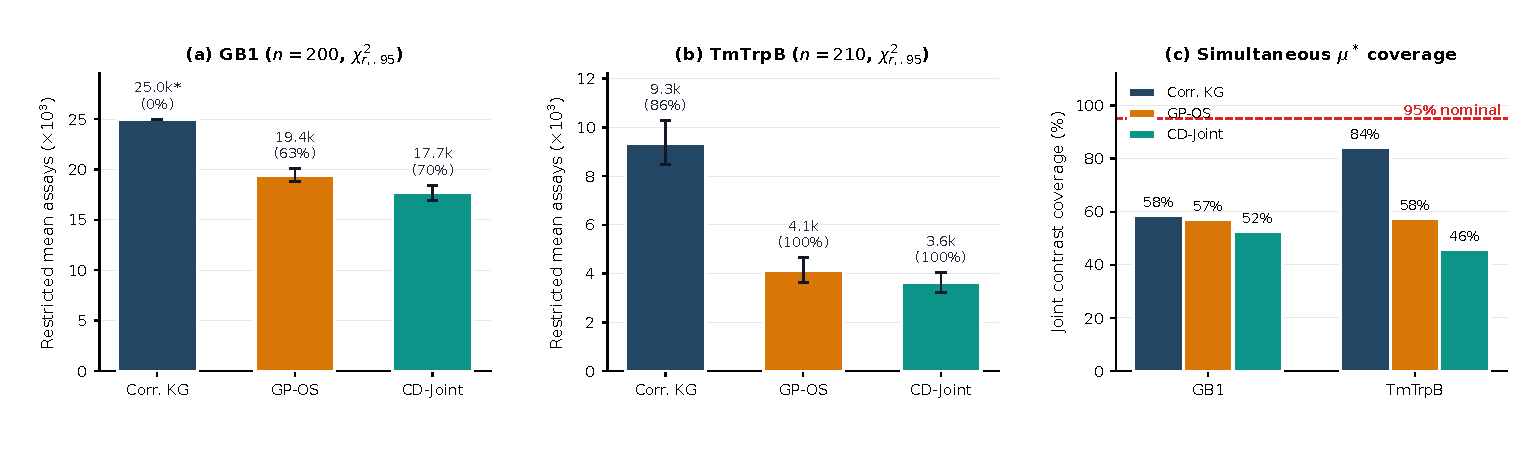
\includegraphics{figures/supp_protein_credibility_audit.pdf}
\vspace{-12pt}
\caption{\textbf{Corrected joint-ellipsoid audit on measured protein landscapes.} (a--b) Restricted mean simulated assays under the $\sqrt{\chi^2_{M-1,.95}}$ joint contrast ellipsoid ($25$k cap), with acquisition policies using the same relevant radius; error bars are $95\%$ bootstrap intervals and labels give the certification rate. (c) Empirical simultaneous coverage of the true mean contrast vector at the stopping time for each policy; all bars remain below the nominal $95\%$ reference. Replotted from Table~\ref{tab:app-v14-protein-credible}. Actual root-decision outcomes, direct-risk stopping, and formal distribution-free controls appear in that table and Figure~\ref{fig:main-results}f--h.}
\label{fig:app-v14-protein-credible}
\end{figure}

\begin{table}[!htbp]
\caption{\textbf{Full $410$-campaign stopping-rule sensitivity and coverage audit on GB1 ($n=200$, $\bar r=486.1$) and TmTrpB ($n=210$, $\bar r=582.3$, $\varepsilon=.015$, $\delta=.05$, cap $25{,}000$).} Reports certification rate, restricted mean assays [95\% bootstrap CI], median certified assays, paired \textsc{KG/Method} and \textsc{Method/CD} ratios [95\% paired bootstrap CIs], false certificates (CP95 upper bound), max actual root regret, empirical root-regret bound coverage (\textsc{RCov}), and exact joint contrast-ellipsoid coverage of $\mu^*$ (\textsc{JCov}). Under Cond.\ B, CD-Joint beats KG on $7/7$ certifiable GB1 templates ($3$ templates capped for all methods) and $21/21$ TmTrpB templates ($2.14\times$--$3.25\times$), and beats GP-OS on $7/7$ non-tied GB1 and $19/21$ TmTrpB templates.}
\label{tab:app-v14-protein-credible}
\uniformaligntable{0.92}{%
\begin{tabular}{@{}lllrrrrrrr@{}}
\toprule
\textbf{Data / Cond.} & \textbf{Policy} & \textbf{Cert.\ (\%)} & \textbf{Restr.\ Mean [95\% CI]} & \textbf{Med.\ OK} & \textbf{KG/m [CI]} & \textbf{m/CD [CI]} & \textbf{Err.\ (CP95)} & \textbf{Max Reg.} & \textbf{RCov / JCov} \\
\midrule
\multirow{3}{*}{GB1 A (nom.)}
 & \textsc{Correlated KG} & $89.5$ & $6{,}983$ [$6{,}001,8{,}018$] & $3{,}040$ & $1.00\times$ & $5.75\times$ $[5.32,6.20]$ & $0/200$ ($\le 1.5\%$) & $.0000$ & $100\% / 0.0\%$ \\
 & \textsc{Correlated GP-OS} & $\mathbf{100.0}$ & $1{,}336$ [$1{,}188,1{,}501$] & $910$ & $5.23\times$ $[4.89,5.56]$ & $1.10\times$ $[1.06,1.14]$ & $0/200$ ($\le 1.5\%$) & $.0000$ & $100\% / 0.0\%$ \\
 & \textsc{CD-Joint} & $\mathbf{100.0}$ & $\mathbf{1{,}214}$ [$1{,}074,1{,}368$] & $\mathbf{800}$ & $\mathbf{5.75\times}$ $[5.31,6.20]$ & $1.00\times$ & $\mathbf{0/200}$ ($\le 1.5\%$) & $.0000$ & $100\% / 0.0\%$ \\
\midrule
\multirow{3}{*}{GB1 B ($\chi^2_{.95}$)}
 & \textsc{Correlated KG} & $0.0$ & $25{,}000^*$ [$25{,}000,25{,}000$] & --- & $1.00\times$ & $1.41\times$ $[1.35,1.48]$ & $0/200$ ($\le 1.5\%$) & $.0071$ & $100\% / 58.5\%$ \\
 & \textsc{Correlated GP-OS} & $63.0$ & $19{,}450$ [$18{,}798,20{,}104$] & $16{,}470$ & $1.29\times$ $[1.24,1.33]$ & $1.10\times$ $[1.09,1.12]$ & $0/200$ ($\le 1.5\%$) & $.0071$ & $100\% / 57.0\%$ \\
 & \textsc{CD-Joint} & $\mathbf{70.0}$ & $\mathbf{17{,}678}$ [$16{,}902,18{,}441$] & $\mathbf{13{,}890}$ & $\mathbf{1.41\times}$ $[1.35,1.48]$ & $1.00\times$ & $\mathbf{0/200}$ ($\le 1.5\%$) & $.0071$ & $100\% / 52.5\%$ \\
\midrule
\multirow{3}{*}{GB1 C ($\chi^2_{.90}$)}
 & \textsc{Correlated KG} & $0.0$ & $25{,}000^*$ [$25{,}000,25{,}000$] & --- & $1.00\times$ & $1.44\times$ $[1.37,1.50]$ & $0/200$ ($\le 1.5\%$) & $.0071$ & $100\% / 50.0\%$ \\
 & \textsc{Correlated GP-OS} & $66.0$ & $19{,}158$ [$18{,}483,19{,}835$] & $16{,}130$ & $1.31\times$ $[1.26,1.35]$ & $1.10\times$ $[1.09,1.12]$ & $0/200$ ($\le 1.5\%$) & $.0071$ & $100\% / 52.0\%$ \\
 & \textsc{CD-Joint} & $\mathbf{70.0}$ & $\mathbf{17{,}418}$ [$16{,}636,18{,}203$] & $\mathbf{13{,}600}$ & $\mathbf{1.44\times}$ $[1.37,1.51]$ & $1.00\times$ & $\mathbf{0/200}$ ($\le 1.5\%$) & $.0071$ & $100\% / 47.5\%$ \\
\midrule
GB1 B$_{\rm frz}$ & \textsc{GP-OS} / \textsc{CD-Joint} & $0.0 / 0.0$ & $25{,}000^* / 25{,}000^*$ & --- & $1.00\times / 1.00\times$ & $1.00\times$ & $0/200$ & $.000/.113$ & $100\% / 66/64\%$ \\
\midrule
\multirow{3}{*}{GB1 E (risk)}
 & \textsc{Correlated KG} & $\mathbf{100.0}$ & $\mathbf{129.7}$ [$119.9,141.3$] & $\mathbf{110}$ & $1.00\times$ & $0.54\times$ $[.49,.60]$ & $9/200$ ($\le 7.7\%$) & $.1097$ & $95.5\% / \text{---}$ \\
 & \textsc{Correlated GP-OS} & $\mathbf{100.0}$ & $223.4$ [$202.7,247.6$] & $190$ & $0.58\times$ $[.52,.65]$ & $0.93\times$ $[.88,.99]$ & $\mathbf{3/200}$ ($\le 3.8\%$) & $.0919$ & $98.5\% / \text{---}$ \\
 & \textsc{CD-Joint} & $\mathbf{100.0}$ & $239.5$ [$222.4,258.2$] & $210$ & $0.54\times$ $[.49,.60]$ & $1.00\times$ & $6/200$ ($\le 5.8\%$) & $.0987$ & $97.0\% / \text{---}$ \\
\midrule
\midrule
\multirow{3}{*}{TrpB A (nom.)}
 & \textsc{Correlated KG} & $\mathbf{100.0}$ & $1{,}056$ [$813,1{,}317$] & $310$ & $1.00\times$ & $3.71\times$ $[3.16,4.21]$ & $0/210$ ($\le 1.4\%$) & $.0000$ & $100\% / 0.0\%$ \\
 & \textsc{Correlated GP-OS} & $\mathbf{100.0}$ & $305.7$ [$269.7,344.9$] & $210$ & $3.46\times$ $[2.98,3.85]$ & $1.08\times$ $[1.04,1.11]$ & $0/210$ ($\le 1.4\%$) & $.0000$ & $100\% / 0.0\%$ \\
 & \textsc{CD-Joint} & $\mathbf{100.0}$ & $\mathbf{284.3}$ [$255.7,315.1$] & $\mathbf{200}$ & $\mathbf{3.71\times}$ $[3.14,4.21]$ & $1.00\times$ & $\mathbf{0/210}$ ($\le 1.4\%$) & $.0000$ & $100\% / 0.0\%$ \\
\midrule
\multirow{3}{*}{TrpB B ($\chi^2_{.95}$)}
 & \textsc{Correlated KG} & $85.7$ & $9{,}337$ [$8{,}459,10{,}264$] & $7{,}500$ & $1.00\times$ & $2.57\times$ $[2.51,2.64]$ & $0/210$ ($\le 1.4\%$) & $.0000$ & $100\% / 84.3\%$ \\
 & \textsc{Correlated GP-OS} & $\mathbf{100.0}$ & $4{,}122$ [$3{,}617,4{,}662$] & $2{,}900$ & $2.27\times$ $[2.20,2.35]$ & $1.14\times$ $[1.11,1.16]$ & $0/210$ ($\le 1.4\%$) & $.0000$ & $100\% / 57.6\%$ \\
 & \textsc{CD-Joint} & $\mathbf{100.0}$ & $\mathbf{3{,}629}$ [$3{,}235,4{,}050$] & $\mathbf{2{,}680}$ & $\mathbf{2.57\times}$ $[2.51,2.64]$ & $1.00\times$ & $\mathbf{0/210}$ ($\le 1.4\%$) & $.0000$ & $100\% / 45.7\%$ \\
\midrule
\multirow{3}{*}{TrpB C ($\chi^2_{.90}$)}
 & \textsc{Correlated KG} & $85.7$ & $9{,}200$ [$8{,}317,10{,}133$] & $7{,}290$ & $1.00\times$ & $2.60\times$ $[2.54,2.66]$ & $0/210$ ($\le 1.4\%$) & $.0000$ & $100\% / 74.8\%$ \\
 & \textsc{Correlated GP-OS} & $\mathbf{100.0}$ & $4{,}030$ [$3{,}536,4{,}561$] & $2{,}840$ & $2.28\times$ $[2.22,2.36]$ & $1.14\times$ $[1.11,1.16]$ & $0/210$ ($\le 1.4\%$) & $.0000$ & $100\% / 50.0\%$ \\
 & \textsc{CD-Joint} & $\mathbf{100.0}$ & $\mathbf{3{,}541}$ [$3{,}158,3{,}948$] & $\mathbf{2{,}630}$ & $\mathbf{2.60\times}$ $[2.54,2.66]$ & $1.00\times$ & $\mathbf{0/210}$ ($\le 1.4\%$) & $.0000$ & $100\% / 40.0\%$ \\
\midrule
TrpB B$_{\rm frz}$ & \textsc{GP-OS} / \textsc{CD-Joint} & $0.0 / 0.0$ & $25{,}000^* / 25{,}000^*$ & --- & $0.37\times / 0.37\times$ & $1.00\times$ & $0/210$ & $.000/.084$ & $100\% / 15/10\%$ \\
\midrule
\multirow{3}{*}{TrpB E (risk)}
 & \textsc{Correlated KG} & $\mathbf{100.0}$ & $\mathbf{62.8}$ [$55.8,70.3$] & $\mathbf{40}$ & $1.00\times$ & $0.68\times$ $[.62,.74]$ & $6/210$ ($\le 5.6\%$) & $.0595$ & $97.1\% / \text{---}$ \\
 & \textsc{Correlated GP-OS} & $\mathbf{100.0}$ & $83.7$ [$74.0,93.8$] & $60$ & $0.75\times$ $[.69,.82]$ & $0.91\times$ $[.84,.97]$ & $\mathbf{5/210}$ ($\le 4.9\%$) & $.0620$ & $97.6\% / \text{---}$ \\
 & \textsc{CD-Joint} & $\mathbf{100.0}$ & $92.5$ [$84.2,101.5$] & $70$ & $0.68\times$ $[.62,.74]$ & $1.00\times$ & $11/210$ ($\le 8.5\%$) & $.0668$ & $94.8\% / \text{---}$ \\
\bottomrule
\end{tabular}%
}
\par\vspace{2pt}\noindent
\parbox{\linewidth}{\scriptsize Paired \textsc{CD/KG} ratios under Cond.\ B ($\chi^2_{r,.95}$): GB1 $=0.707$ $[.677,.738]$ (lower-bounded by $100\%$ KG capping), TrpB $=0.389$ $[.379,.398]$; under Cond.\ C: $0.697$ $[.665,.728]$ / $0.385$ $[.376,.394]$. Mean actual root regret is $\le 0.0004$ across Conds.\ A--C and $0.0007$--$0.0035$ under Cond.\ E. Cond.\ C$_{\rm frz}$ matches B$_{\rm frz}$ ($0\%$ cert.\ for frozen GP-OS/CD-Joint). Self-contained Cond.\ D (formal DF) matches Table~\ref{tab:app-v13-regime-b} bit-for-bit.}
\end{table}

\subsection{Nominal-radius and distribution-free acquisition controls}

\paragraph{Scope of the application acquisition comparisons.}
The matched retrospective GB1 and TmTrpB comparison includes a direct, paired comparison of CD-Joint, correlated KG, and other root-aware acquisitions using the same fixed sequence-kernel GP and two common stopping rules (Appendix~\ref{app:v13-protein}). The nominal GP conic rule is an \emph{uncalibrated model-based stopping criterion}; the independent-arm empirical-Bernstein rule has its separate anytime-valid coverage guarantee. These comparisons establish acquisition efficiency conditional on the stated rule, not transfer of a theoretical Gaussian credible-set guarantee to bounded non-Gaussian protein observations.

\begin{table}[!htbp]
\caption{\textbf{Regime A — Matched GP-model-based stopping on GB1 ($n=200$) and TmTrpB ($n=210$) across $\varepsilon\in\{.015,.010\}$ ($\delta=.05$, cap $25{,}000$, identical fixed GP working model and nominal conic criterion (not established to have $1-\delta$ joint coverage)).} Reports certification rate, restricted mean assays [95\% bootstrap CI], median among certified runs, paired \textsc{CD/KG} and \textsc{KG/Method} ratios [95\% paired bootstrap CIs], false certificates ($0/200$ CP95 $\le 1.49\%$; $0/210$ CP95 $\le 1.42\%$), pointwise GP coverage at stopping, and mean acquisition time (s / ms per step).}
\label{tab:app-v13-regime-a}
\uniformaligntable{0.92}{%
\begin{tabular}{@{}lllrrrrrrr@{}}
\toprule
\textbf{$\varepsilon$ / Data} & \textbf{Policy} & \textbf{Cert.\ (\%)} & \textbf{Restr.\ Mean [95\% CI]} & \textbf{Med.\ OK} & \textbf{vs.\ KG (KG/m) [CI]} & \textbf{m / CD [CI]} & \textbf{Err.\ (PW Cov.)} & \textbf{Acq.\ s (ms/st)} \\
\midrule
\multirow{5}{*}{$.015$ GB1}
 & \textsc{GP-UCB} & $37.5$ & $23{,}604$ [$23{,}272,23{,}920$] & $21{,}780$ & $0.30\times$ $[.26,.34]$ & $19.4\times$ $[17.3,22.0]$ & $0/200$ ($100\%$) & $1.06$ ($0.045$) \\
 & \textsc{Correlated KG} & $89.5$ & $6{,}983$ [$6{,}039,8{,}012$] & $3{,}040$ & $1.00\times$ & $5.75\times$ $[5.32,6.20]$ & $0/200$ ($99.4\%$) & $25.60$ ($3.667$) \\
 & \textsc{GP-Root-Info} & $\mathbf{100.0}$ & $1{,}407$ [$1{,}238,1{,}596$] & $895$ & $4.96\times$ $[4.50,5.43]$ & $1.16\times$ $[1.09,1.25]$ & $0/200$ ($100\%$) & $\mathbf{0.11}$ ($0.078$) \\
 & \textsc{Correlated GP-OS} & $\mathbf{100.0}$ & $1{,}336$ [$1{,}191,1{,}497$] & $910$ & $5.23\times$ $[4.90,5.57]$ & $1.10\times$ $[1.06,1.14]$ & $0/200$ ($100\%$) & $0.37$ ($0.276$) \\
 & \textsc{CD-Joint} & $\mathbf{100.0}$ & $\mathbf{1{,}214}$ [$1{,}074,1{,}368$] & $\mathbf{800}$ & $\mathbf{5.75\times}$ $[5.32,6.20]$ & $1.00\times$ & $\mathbf{0/200}$ ($100\%$) & $2.13$ ($1.755$) \\
\midrule
\multirow{5}{*}{$.015$ TrpB}
 & \textsc{GP-UCB} & $\mathbf{100.0}$ & $1{,}266$ [$1{,}200,1{,}332$] & $1{,}160$ & $0.83\times$ $[.66,1.02]$ & $4.45\times$ $[4.10,4.86]$ & $0/210$ ($100\%$) & $0.08$ ($0.060$) \\
 & \textsc{Correlated KG} & $\mathbf{100.0}$ & $1{,}056$ [$811,1{,}321$] & $310$ & $1.00\times$ & $3.71\times$ $[3.16,4.22]$ & $0/210$ ($100\%$) & $5.73$ ($5.429$) \\
 & \textsc{GP-Root-Info} & $\mathbf{100.0}$ & $305.3$ [$269.6,344.8$] & $\mathbf{200}$ & $3.46\times$ $[3.01,3.84]$ & $1.07\times$ $[1.03,1.11]$ & $0/210$ ($99.5\%$) & $\mathbf{0.03}$ ($0.102$) \\
 & \textsc{Correlated GP-OS} & $\mathbf{100.0}$ & $305.7$ [$270.2,344.1$] & $210$ & $3.46\times$ $[3.00,3.86]$ & $1.08\times$ $[1.04,1.11]$ & $0/210$ ($100\%$) & $0.11$ ($0.355$) \\
 & \textsc{CD-Joint} & $\mathbf{100.0}$ & $\mathbf{284.3}$ [$255.4,315.6$] & $\mathbf{200}$ & $\mathbf{3.71\times}$ $[3.14,4.22]$ & $1.00\times$ & $\mathbf{0/210}$ ($100\%$) & $0.76$ ($2.673$) \\
\midrule
\multirow{5}{*}{$.010$ GB1}
 & \textsc{GP-UCB} & $0.0$ & $25{,}000^*$ [$25{,}000,25{,}000$] & --- & $0.30\times$ $[.26,.34]$ & $18.8\times$ $[16.4,21.7]$ & $0/200$ ($100\%$) & $1.12$ ($0.045$) \\
 & \textsc{Correlated KG} & $89.0$ & $7{,}440$ [$6{,}474,8{,}478$] & $3{,}370$ & $1.00\times$ & $5.58\times$ $[5.19,6.01]$ & $0/200$ ($100\%$) & $27.40$ ($3.683$) \\
 & \textsc{GP-Root-Info} & $\mathbf{100.0}$ & $1{,}587$ [$1{,}363,1{,}844$] & $910$ & $4.69\times$ $[4.21,5.19]$ & $1.19\times$ $[1.10,1.32]$ & $0/200$ ($100\%$) & $\mathbf{0.12}$ ($0.077$) \\
 & \textsc{Correlated GP-OS} & $\mathbf{100.0}$ & $1{,}478$ [$1{,}292,1{,}684$] & $950$ & $5.03\times$ $[4.71,5.39]$ & $1.11\times$ $[1.08,1.14]$ & $0/200$ ($100\%$) & $0.41$ ($0.276$) \\
 & \textsc{CD-Joint} & $\mathbf{100.0}$ & $\mathbf{1{,}332}$ [$1{,}160,1{,}522$] & $\mathbf{815}$ & $\mathbf{5.58\times}$ $[5.19,6.02]$ & $1.00\times$ & $\mathbf{0/200}$ ($100\%$) & $2.28$ ($1.707$) \\
\midrule
\multirow{5}{*}{$.010$ TrpB}
 & \textsc{GP-UCB} & $\mathbf{100.0}$ & $2{,}944$ [$2{,}743,3{,}151$] & $2{,}730$ & $0.48\times$ $[.36,.61]$ & $9.49\times$ $[8.45,10.7]$ & $0/210$ ($100\%$) & $0.17$ ($0.056$) \\
 & \textsc{Correlated KG} & $\mathbf{100.0}$ & $1{,}422$ [$1{,}063,1{,}808$] & $330$ & $1.00\times$ & $4.58\times$ $[3.86,5.22]$ & $0/210$ ($100\%$) & $7.68$ ($5.402$) \\
 & \textsc{GP-Root-Info} & $\mathbf{100.0}$ & $333.7$ [$289.9,381.9$] & $210$ & $4.26\times$ $[3.66,4.74]$ & $1.08\times$ $[1.04,1.11]$ & $0/210$ ($99.5\%$) & $\mathbf{0.03}$ ($0.103$) \\
 & \textsc{Correlated GP-OS} & $\mathbf{100.0}$ & $333.4$ [$290.0,380.4$] & $220$ & $4.26\times$ $[3.67,4.78]$ & $1.08\times$ $[1.04,1.11]$ & $0/210$ ($100\%$) & $0.12$ ($0.358$) \\
 & \textsc{CD-Joint} & $\mathbf{100.0}$ & $\mathbf{310.1}$ [$273.1,350.1$] & $\mathbf{200}$ & $\mathbf{4.58\times}$ $[3.85,5.22]$ & $1.00\times$ & $\mathbf{0/210}$ ($100\%$) & $0.79$ ($2.561$) \\
\bottomrule
\multicolumn{9}{@{}l@{}}{\scriptsize Paired \textsc{CD/KG} ratios: GB1 $.015$ = $0.174$ $[.162,.188]$, $.010$ = $0.179$ $[.167,.193]$; TrpB $.015$ = $0.269$ $[.238,.319]$, $.010$ = $0.218$ $[.192,.261]$. Recorded maximal root regret among returned actions in $2{,}050$ nominal GP-based stopping runs is $0.00000$; empirical errors do not establish calibrated coverage.}
\end{tabular}%
}
\end{table}

\begin{table}[!htbp]
\caption{\textbf{Regime B — Formal distribution-free Empirical Bernstein stopping on GB1 ($n=200$) and TmTrpB ($n=210$) across $\varepsilon\in\{.015,.010\}$ ($\delta=.05$, cap $25{,}000$, $0/8{,}200$ errors).} Top block of each dataset shows unmodified GP-only acquisitions (blind to DF intervals); bottom block shows DF-coupled \textsc{GP-Root-Info}, two-phase DF-confirmed handoffs (\textsc{CD-Joint}/\textsc{GP-OS}/\textsc{KG} $\to$ \textsc{DF-OS}), and zero-GP \textsc{DF-OS}.}
\label{tab:app-v13-regime-b}
\uniformaligntable{0.92}{%
\begin{tabular}{@{}llrrrrrr@{}}
\toprule
\textbf{Data / $\varepsilon$} & \textbf{Policy (DF Emp.\ Bern.\ Stop)} & \textbf{Cert.\ (\%)} & \textbf{Restr.\ Mean [95\% CI]} & \textbf{Med.\ OK} & \textbf{DF-OS / m [CI]} & \textbf{Mean Reg.\ (Dist.\ Arms)} & \textbf{Acq.\ s} \\
\midrule
\multirow{8}{*}{GB1 $.015$}
 & \textsc{GP-UCB} / \textsc{GP-Root-Info} / \textsc{GP-OS} (GP-only) & $0.0$ & $25{,}000^*$ [$25{,}000,25{,}000$] & --- & $0.61\times$ $[.60,.63]$ & $.0000$ ($376 / 437 / 445$) & $1.1/1.8/6.7$ \\
 & \textsc{CD-Joint} (GP-only) & $0.0$ & $25{,}000^*$ [$25{,}000,25{,}000$] & --- & $0.61\times$ $[.60,.63]$ & $.0063$ ($439$) & $15.82$ \\
 & \textsc{Correlated KG} (GP-only) & $65.5$ & $20{,}102$ [$19{,}505,20{,}700$] & $16{,}457$ & $0.76\times$ $[.75,.77]$ & $.0000$ ($487$) & $72.28$ \\
 \cmidrule(lr){2-8}
 & \textsc{KG} $\to$ \textsc{DF-OS} (2-phase) & $88.0$ & $16{,}104$ [$15{,}514,16{,}703$] & $13{,}724$ & $0.95\times$ $[.93,.97]$ & $.0000$ ($487$) & $25.62$ \\
 & \textsc{CD-Joint} $\to$ \textsc{DF-OS} (2-phase) & $\mathbf{100.0}$ & $15{,}307$ [$14{,}888,15{,}722$] & $13{,}895$ & $1.00\times$ $[1.00,1.00]$ & $.0000$ ($486$) & $2.16$ \\
 & \textsc{GP-OS} $\to$ \textsc{DF-OS} (2-phase) & $\mathbf{100.0}$ & $15{,}295$ [$14{,}898,15{,}710$] & $13{,}890$ & $1.00\times$ $[1.00,1.00]$ & $.0000$ ($486$) & $0.40$ \\
 & \textsc{GP-Root-Info} (DF-coupled) & $\mathbf{100.0}$ & $\mathbf{14{,}860}$ [$14{,}465,15{,}262$] & $\mathbf{13{,}520}$ & $\mathbf{1.03\times}$ $[1.03,1.03]$ & $.0000$ ($485$) & $2.71$ \\
 & \textsc{DF-OS} (zero-GP reference) & $\mathbf{100.0}$ & $15{,}292$ [$14{,}887,15{,}691$] & $13{,}890$ & $1.00\times$ & $.0000$ ($486$) & $\mathbf{0.01}$ \\
\midrule
\multirow{8}{*}{TrpB $.015$}
 & \textsc{GP-UCB} / \textsc{GP-Root-Info} / \textsc{GP-OS} (GP-only) & $0.0$ & $25{,}000^*$ [$25{,}000,25{,}000$] & --- & $0.68\times$ $[.66,.69]$ & $.0000$ ($209 / 314 / 322$) & $1.3/2.2/8.0$ \\
 & \textsc{CD-Joint} (GP-only) & $0.0$ & $25{,}000^*$ [$25{,}000,25{,}000$] & --- & $0.68\times$ $[.66,.69]$ & $.0119$ ($309$) & $20.58$ \\
 & \textsc{Correlated KG} (GP-only) & $85.7$ & $17{,}184$ [$16{,}721,17{,}682$] & $15{,}681$ & $0.99\times$ $[.98,1.00]$ & $.0000$ ($583$) & $87.00$ \\
 \cmidrule(lr){2-8}
 & \textsc{KG} $\to$ \textsc{DF-OS} (2-phase) & $\mathbf{100.0}$ & $16{,}932$ [$16{,}543,17{,}342$] & $16{,}313$ & $1.00\times$ $[1.00,1.00]$ & $.0000$ ($580$) & $5.77$ \\
 & \textsc{CD-Joint} $\to$ \textsc{DF-OS} (2-phase) & $\mathbf{100.0}$ & $16{,}924$ [$16{,}527,17{,}324$] & $16{,}304$ & $1.00\times$ $[1.00,1.00]$ & $.0000$ ($577$) & $0.80$ \\
 & \textsc{GP-OS} $\to$ \textsc{DF-OS} (2-phase) & $\mathbf{100.0}$ & $16{,}928$ [$16{,}531,17{,}339$] & $16{,}313$ & $1.00\times$ $[1.00,1.00]$ & $.0000$ ($578$) & $0.15$ \\
 & \textsc{GP-Root-Info} (DF-coupled) & $\mathbf{100.0}$ & $\mathbf{16{,}399}$ [$16{,}101,16{,}709$] & $\mathbf{16{,}225}$ & $\mathbf{1.03\times}$ $[1.03,1.04]$ & $.0000$ ($578$) & $3.77$ \\
 & \textsc{DF-OS} (zero-GP reference) & $\mathbf{100.0}$ & $16{,}925$ [$16{,}535,17{,}326$] & $16{,}313$ & $1.00\times$ & $.0000$ ($576$) & $\mathbf{0.02}$ \\
\midrule
\multirow{2}{*}{$.010$ Sens.}
 & GB1: \textsc{KG} / \textsc{CD} (GP) / \textsc{CD}$\to$\textsc{DF} / \textsc{GRI-DF} / \textsc{DF-OS} & $62/0/99/\mathbf{100}/99$ & $20{,}361 / 25{,}000^* / 15{,}612 / \mathbf{15{,}175} / 15{,}605$ & $16.7/$-$/14.0/\mathbf{13.6}/14.0$k & $1.03\times$ (GRI) & $0/200$ err.\ all & --- \\
 & TrpB: \textsc{KG} / \textsc{CD} (GP) / \textsc{CD}$\to$\textsc{DF} / \textsc{GRI-DF} / \textsc{DF-OS} & $86/0/99/\mathbf{100}/99$ & $17{,}408 / 25{,}000^* / 17{,}109 / \mathbf{16{,}555} / 17{,}109$ & $16.0/$-$/16.4/\mathbf{16.3}/16.4$k & $1.03\times$ (GRI) & $0/210$ err.\ all & --- \\
\bottomrule
\end{tabular}%
}
\end{table}

\subsection{Decision-level calibration and stopping-rule ablations}
\label{app:v11-audit}

The certificate-validity factorial and fixed-trajectory stopping replay use raw GB1 ($n=200$) and TmTrpB ($n=210$), with $10{,}000$-resample paired bootstrap $95\%$ intervals and separate terminal-coverage and decision-regret diagnostics. Table~\ref{tab:app-v11-protein} reports these results. The live workflow replication and independent oracle audit are reported in Sections~\ref{app:group-workflows} and~\ref{app:group-benchmarks}.

\begin{table}[!htbp]
\caption{\textbf{Real-data certificate-validity factorial (top) and exact fixed-trajectory coupled-stream stopping replay (bottom) on raw GB1 ($10$ templates $\times 20$ seeds $=200$) and raw TmTrpB ($21$ templates $\times 10$ seeds $=210$, $\varepsilon=.015$, $\delta=.05$, caps $12$k and $25$k).} Ratios report uncensored $25$k median ratios vs.\ \textsc{OS (DF)} (or vs.\ DF on the identical fixed stream) with $10{,}000$-resample paired bootstrap $95\%$ CIs; all rows observed $0/200$ GB1 (CP95 $\le 1.49\%$) and $0/210$ TmTrpB (CP95 $\le 1.42\%$) false certifications. \emph{Pointwise cov.} measures simultaneous GP box coverage across all $381$ sequences at stopping, whereas \emph{Reg.\ cov.} measures decision-level regret-bound coverage ($R_t(a_{\mathrm{cert}})\ge r(a_{\mathrm{cert}})$).}
\label{tab:app-v11-protein}
\uniformaligntable{0.93}{%
\begin{tabular}{@{}lllrrrrrr@{}}
\toprule
\textbf{Study / Landscape} & \textbf{Method / Stopping Rule} & \textbf{Validity Tier} & \textbf{Cert.\ 12k/25k} & \textbf{Med.\ 25k [IQR]} & \textbf{Ratio vs.\ OS [95\% CI]} & \textbf{Err.} & \textbf{Pw.\ Cov.} & \textbf{Reg.\ Cov.} \\
\midrule
\multirow{7}{*}{GB1 Interactive ($200$)}
 & \textsc{os\_df\_stop} & Formal DF & $5.5\%/100\%$ & $13{,}890$ $[13.3,18.5]$k & $1.00\times$ $[1.00,1.00]$ & $0$ & $100\%$ & $100\%$ \\
 & \textsc{eb\_pure\_df\_stop} & Formal DF & $0.0\%/0.0\%$ & $25{,}000^*$ $[25.0,25.0]$k & $0.56\times$ $[0.55,0.57]$ & $0$ & $100\%$ & $100\%$ \\
 & \textsc{eb\_warmup\_os\_df} & Formal DF & $6.5\%/100\%$ & $13{,}891$ $[13.3,18.5]$k & $1.00\times$ $[1.00,1.00]$ & $0$ & $100\%$ & $100\%$ \\
 & \textsc{eb\_and\_df\_strict} & Formal DF (strict) & $4.0\%/99.0\%$ & $15{,}443$ $[13.6,18.7]$k & $0.90\times$ $[0.88,0.94]$ & $0$ & $100\%$ & $100\%$ \\
 & \textsc{eb\_acq\_rob005} & Valid $|b|\le.005$ & $55.5\%/77.0\%$ & $10{,}620$ $[3.0,16.8]$k & $1.31\times$ $[1.14,2.17]$ & $0$ & $100\%$ & $100\%$ \\
 & \textsc{eb\_acq\_rob005\_or\_df} & Valid $|b|\le.005$ fb. & $0.5\%/100\%$ & $14{,}878$ $[14.2,19.8]$k & $0.93\times$ $[0.93,0.94]$ & $0$ & $100\%$ & $100\%$ \\
 & \textsc{eb\_acq\_eb\_stop} & Model-based (EB) & $91.0\%/99.5\%$ & $\mathbf{2{,}895}$ $[1.8,6.4]$k & $\mathbf{4.80\times}$ $[3.83,5.61]$ & $0$ & $\mathbf{91.5\%}$ & $100\%$ \\
\midrule
\multirow{7}{*}{TmTrpB Interactive ($210$)}
 & \textsc{os\_df\_stop} & Formal DF & $0.0\%/100\%$ & $16{,}313$ $[14.6,17.3]$k & $1.00\times$ $[1.00,1.00]$ & $0$ & $100\%$ & $100\%$ \\
 & \textsc{eb\_pure\_df\_stop} & Formal DF & $0.0\%/0.0\%$ & $25{,}000^*$ $[25.0,25.0]$k & $0.65\times$ $[0.65,0.66]$ & $0$ & $100\%$ & $100\%$ \\
 & \textsc{eb\_warmup\_os\_df} & Formal DF & $0.0\%/100\%$ & $16{,}314$ $[14.6,17.3]$k & $1.00\times$ $[1.00,1.00]$ & $0$ & $100\%$ & $100\%$ \\
 & \textsc{eb\_and\_df\_strict} & Formal DF (strict) & $0.0\%/98.6\%$ & $16{,}810$ $[15.4,19.5]$k & $0.97\times$ $[0.96,0.98]$ & $0$ & $100\%$ & $100\%$ \\
 & \textsc{eb\_acq\_rob005} & Valid $|b|\le.005$ & $26.2\%/60.5\%$ & $15{,}360$ $[9.2,25.0]$k & $1.06\times$ $[1.02,1.09]$ & $0$ & $100\%$ & $100\%$ \\
 & \textsc{eb\_acq\_rob005\_or\_df} & Valid $|b|\le.005$ fb. & $0.0\%/93.3\%$ & $17{,}402$ $[15.6,18.5]$k & $0.94\times$ $[0.94,0.94]$ & $0$ & $100\%$ & $100\%$ \\
 & \textsc{eb\_acq\_eb\_stop} & Model-based (EB) & $85.7\%/100\%$ & $\mathbf{4{,}410}$ $[2.3,6.5]$k & $\mathbf{3.70\times}$ $[3.37,4.35]$ & $0$ & $\mathbf{82.9\%}$ & $100\%$ \\
\midrule
\multirow{4}{*}{GB1 Replay (Fixed Stream)}
 & \textsc{os\_stream}: DF / \textsc{Rob.005} & Formal DF / $|b|\le\xi$ & $100\% / 55.0\%$ & $13{,}890$ / $13{,}380$ & $1.04\times$ $[1.02,1.06]$ & $0/0$ & $100\%$ & $100\%$ \\
 & \textsc{os\_stream}: \textsc{Calib.\ EB+LOO} & Model-based (EB) & $99.5\%$ & $10{,}680$ $[9.5,15.4]$k & $1.30\times$ $[1.26,1.35]$ & $0$ & $98.0\%$ & $100\%$ \\
 & \textsc{eb\_stream}: DF / \textsc{Rob.005} & Formal DF / $|b|\le\xi$ & $0.0\% / 21.0\%$ & $25{,}000^*$ / $25{,}000^*$ & --- (DF stalled) & $0/0$ & $97.6\%$ & $100\%$ \\
 & \textsc{eb\_stream}: \textsc{Calib.\ EB+LOO} & Model-based (EB) & $99.5\%$ & $\mathbf{2{,}910}$ $[1.8,6.4]$k & $99.5\%$ vs.\ $0\%$ (DF cap) & $0$ & $91.5\%$ & $100\%$ \\
\midrule
\multirow{4}{*}{TrpB Replay (Fixed Stream)}
 & \textsc{os\_stream}: DF / \textsc{Rob.005} & Formal DF / $|b|\le\xi$ & $100\% / 70.5\%$ & $16{,}313$ / $12{,}690$ & $1.29\times$ $[1.26,1.31]$ & $0/0$ & $100\%$ & $100\%$ \\
 & \textsc{os\_stream}: \textsc{Calib.\ EB+LOO} & Model-based (EB) & $100.0\%$ & $10{,}080$ $[9.4,10.6]$k & $1.62\times$ $[1.61,1.65]$ & $0$ & $91.9\%$ & $100\%$ \\
 & \textsc{eb\_stream}: DF / \textsc{Rob.005} & Formal DF / $|b|\le\xi$ & $0.0\% / 1.4\%$ & $25{,}000^*$ / $25{,}000^*$ & --- (DF stalled) & $0/0$ & $100\%$ & $100\%$ \\
 & \textsc{eb\_stream}: \textsc{Calib.\ EB+LOO} & Model-based (EB) & $100.0\%$ & $\mathbf{4{,}440}$ $[2.4,6.5]$k & $100\%$ vs.\ $0\%$ (DF cap) & $0$ & $82.4\%$ & $100\%$ \\
\bottomrule
\end{tabular}%
}
\end{table}

\begin{table}[!htbp]
\caption{\textbf{High-power calibrated protein certification across GB1 ($10$ templates $\times 20$ seeds $=200$ runs/method) and complete TmTrpB ($21$ templates $\times 10$ seeds $=210$ runs/method; $\varepsilon=.015, \delta=.05$).} Both the $12$k cap and uncensored $25$k horizon are recorded on each trajectory; \textsc{Calib.\ EB} performs strictly leak-free online Type-II ML kernel selection plus closed-form GP LOO variance inflation; \textsc{Uncert.\ Reg.} reports mean true regret of the best available recommendation across runs uncertified at $12$k.}
\label{tab:app-v8-proteins}
\uniformaligntable{0.92}{%
\begin{tabular}{@{}llrrrrrrrr@{}}
\toprule
\textbf{Landscape} & \textbf{Method} & \textbf{Cert.\ 12k} & \textbf{Med.\ 12k} & \textbf{Cert.\ 25k} & \textbf{Med.\ 25k} & \textbf{Err.} & \textbf{Uncert.\ Reg.} & \textbf{Fit (ms)} & \textbf{Total (ms)} \\
\midrule
\multirow{9}{*}{GB1 ($200$)}
 & \textsc{Indep.\ OS} (DF) & $5.5\%$ & $12{,}000$ & $100.0\%$ & $13{,}890$ & $0/200$ & $.0003$ & $0.0$ & $637.7$ \\
 & \textsc{DF-CD Fallback} (DF) & $6.5\%$ & $12{,}000$ & $100.0\%$ & $13{,}891$ & $0/200$ & $.0003$ & $0.0$ & $1{,}154.5$ \\
 & \textsc{CD-Joint} (Nom.\ GP) & $92.5\%$ & $4{,}515$ & $99.0\%$ & $4{,}515$ & $0/200$ & $.0168$ & $0.0$ & $2{,}204.0$ \\
 & \textsc{CD-Joint} (Calib.\ EB) & $91.0\%$ & $2{,}895$ & $99.5\%$ & $2{,}895$ & $0/200$ & $.0095$ & $74.7$ & $1{,}503.4$ \\
 & \textsc{CD-Joint} (Rob.\ $\xi=.005$) & $55.5\%$ & $10{,}620$ & $77.0\%$ & $10{,}620$ & $0/200$ & $.0098$ & $87.8$ & $3{,}131.0$ \\
 & \textsc{CD-Joint} (Rob.\ $\xi=.010$) & $0.0\%$ & $12{,}000$ & $0.0\%$ & $25{,}000$ & $0/200$ & $.0455$ & $85.5$ & $1{,}168.5$ \\
 & \textsc{CD-Joint} (Hybrid EB) & $70.0\%$ & $\mathbf{2{,}760}$ & $100.0\%$ & $\mathbf{2{,}760}$ & $0/200$ & $.0017$ & $74.3$ & $1{,}634.2$ \\
 & \textsc{CD-Joint} (Hybrid $.005$) & $0.5\%$ & $12{,}000$ & $100.0\%$ & $14{,}878$ & $0/200$ & $.0004$ & $75.0$ & $1{,}335.0$ \\
 & \textsc{CD-Joint} (Hybrid $.010$) & $0.5\%$ & $12{,}000$ & $100.0\%$ & $14{,}878$ & $0/200$ & $.0004$ & $60.9$ & $1{,}125.0$ \\
\midrule
\multirow{9}{*}{TmTrpB ($210$)}
 & \textsc{Indep.\ OS} (DF) & $0.0\%$ & $12{,}000$ & $100.0\%$ & $16{,}313$ & $0/210$ & $.0013$ & $0.0$ & $686.3$ \\
 & \textsc{DF-CD Fallback} (DF) & $0.0\%$ & $12{,}000$ & $100.0\%$ & $16{,}314$ & $0/210$ & $.0013$ & $0.0$ & $1{,}314.0$ \\
 & \textsc{CD-Joint} (Nom.\ GP) & $100.0\%$ & $\mathbf{3{,}795}$ & $100.0\%$ & $\mathbf{3{,}795}$ & $0/210$ & $.0000$ & $0.0$ & $2{,}108.9$ \\
 & \textsc{CD-Joint} (Calib.\ EB) & $85.7\%$ & $4{,}410$ & $100.0\%$ & $4{,}410$ & $0/210$ & $.0061$ & $80.1$ & $2{,}128.8$ \\
 & \textsc{CD-Joint} (Rob.\ $\xi=.005$) & $26.2\%$ & $12{,}000$ & $60.5\%$ & $15{,}360$ & $0/210$ & $.0046$ & $93.7$ & $6{,}961.4$ \\
 & \textsc{CD-Joint} (Rob.\ $\xi=.010$) & $0.0\%$ & $12{,}000$ & $0.0\%$ & $25{,}000$ & $0/210$ & $.0532$ & $92.6$ & $1{,}606.3$ \\
 & \textsc{CD-Joint} (Hybrid EB) & $59.5\%$ & $4{,}965$ & $95.2\%$ & $4{,}965$ & $2/210$ & $.0303$ & $81.1$ & $2{,}670.8$ \\
 & \textsc{CD-Joint} (Hybrid $.005$) & $0.0\%$ & $12{,}000$ & $93.3\%$ & $17{,}402$ & $0/210$ & $.0030$ & $78.8$ & $1{,}573.1$ \\
 & \textsc{CD-Joint} (Hybrid $.010$) & $0.0\%$ & $12{,}000$ & $93.3\%$ & $17{,}402$ & $0/210$ & $.0038$ & $64.7$ & $1{,}305.0$ \\
\bottomrule
\end{tabular}%
}
\end{table}

\subsection{Extended sequence-space, noise, and discovery comparisons}

\begin{table}[!t]
\caption{\textbf{Combinatorial GB1 protein mutagenesis across ten starting variants (five-residue panel \texttt{ACGWY}, $\varepsilon=0.010$, $45{,}000$-assay cap; $6$ paired seeds per cell).} Entries report median capped assays ($^*$ denotes $<100\%$ certified at $45\text{k}$); \emph{Fit$^*$} is measured binding fitness ($\times$ wild-type) of the optimal reachable variant.}
\label{tab:app-gb1-templates}
\uniformaligntable{0.92}{%
\begin{tabular}{@{}lrrrrrrr@{}}
\toprule
\textbf{Start ($M$)} & \textbf{$\Gamma/\Delta_{\mathrm{flat}}$} & \textbf{Fit$^*$} & \textbf{Flat-LUCB} & \textbf{Flat+Root} & \textbf{Exact-UCB} & \textbf{Opt.-Sep} & \textbf{GP-Root} \\
\midrule
\texttt{VDGA} ($467$) & $1.0\times$  & $7.28$ & $21{,}320$   & $21{,}320$   & $20{,}931$ & $21{,}173$ & $\mathbf{20{,}386}$ \\
\texttt{LDGV} ($540$) & $1.5\times$  & $7.23$ & $15{,}558$   & $15{,}555$   & $\mathbf{15{,}297}$ & $15{,}848$ & $15{,}751$ \\
\texttt{VWGV} ($467$) & $2.3\times$  & $7.28$ & $15{,}295$   & $15{,}295$   & $15{,}037$ & $14{,}031$ & $\mathbf{13{,}619}$ \\
\texttt{WDGV} ($460$) & $2.5\times$  & $7.28$ & $12{,}433$   & $12{,}432$   & $\mathbf{12{,}043}$ & $13{,}585$ & $13{,}459$ \\
\texttt{YDGV} ($460$) & $2.6\times$  & $6.98$ & $13{,}655$   & $13{,}654$   & $\mathbf{13{,}318}$ & $13{,}691$ & $13{,}443$ \\
\texttt{FDGV} ($538$) & $3.1\times$  & $8.76$ & $12{,}477$   & $12{,}474$   & $12{,}190$ & $12{,}203$ & $\mathbf{11{,}933}$ \\
\midrule
\texttt{VDGV} ($539$) & $13.2\times$ & $6.20$ & $45{,}000^*$ & $45{,}000^*$ & $18{,}959$ & $19{,}016$ & $\mathbf{18{,}695}$ \\
\texttt{ADGV} ($393$) & $18.8\times$ & $6.50$ & $45{,}000^*$ & $45{,}000^*$ & $12{,}172$ & $12{,}188$ & $\mathbf{11{,}225}$ \\
\texttt{LWGV} ($467$) & $32.9\times$ & $7.28$ & $45{,}000^*$ & $45{,}000^*$ & $13{,}582$ & $13{,}590$ & $\mathbf{13{,}298}$ \\
\texttt{IDGV} ($540$) & $36.0\times$ & $6.04$ & $45{,}000^*$ & $45{,}000^*$ & $30{,}076^*$ & $19{,}784$ & $\mathbf{18{,}879}$ \\
\midrule
Med.\ Assays & --- & $7.08$ & $16{,}932^*$ & $16{,}930^*$ & $14{,}261^*$ & $14{,}030$ & $\mathbf{13{,}688}$ \\
Cert.\ Rate  & --- & ---    & $60.0\%$     & $60.0\%$     & $96.7\%$     & $\mathbf{100\%}$ & $\mathbf{100\%}$ \\
\bottomrule
\end{tabular}%
}
\end{table}

\begin{table}[!t]
\caption{\textbf{GB1 codon-panel scale and overlap sweep across \texttt{FDGV}, \texttt{VDGV}, and \texttt{ADGV} ($336$ runs; $\varepsilon=0.015$, $50{,}000$-assay cap).}}
\label{tab:app-gb1-panels}
\uniformaligntable{0.92}{%
\begin{tabular}{@{}lrrrrrr@{}}
\toprule
\textbf{Codon Panel} & \textbf{Mean $M$} & \textbf{Jaccard} & \textbf{LUCB-m Cert.} & \textbf{Flat-LUCB} & \textbf{Exact-UCB} & \textbf{Opt.-Sep} \\
\midrule
4-AA (\texttt{AGWY})     & $257$   & $0.068$ & $33.3\%$ & $36{,}031\ (67\%)$ & $9{,}395\ (67\%)$  & $\mathbf{9{,}333}\ (67\%)$ \\
5-AA (\texttt{ACGWY})    & $490$   & $0.053$ & $33.3\%$ & $43{,}610\ (67\%)$ & $15{,}571\ (\mathbf{100\%})$ & $\mathbf{12{,}210}\ (\mathbf{100\%})$ \\
6-AA (\texttt{ACFGWY})   & $813$   & $0.045$ & $33.3\%$ & $48{,}759\ (58\%)$ & $42{,}709\ (58\%)$ & $\mathbf{40{,}040}\ (\mathbf{67\%})$ \\
8-AA (\texttt{ACFGLVWY}) & $1{,}765$ & $0.035$ & $0.0\%$  & $50{,}000^*\ (33\%)$ & $50{,}000^*\ (33\%)$ & $50{,}000^*\ (33\%)$ \\
\bottomrule
\end{tabular}%
}
\end{table}

\begin{table}[!t]
\caption{\textbf{GB1 observation-model sensitivity ($600$ runs across $10$ templates) and unselected $21$-template TmTrpB enzyme benchmark ($420$ runs; $\varepsilon=0.010$, $45{,}000$-assay cap).}}
\label{tab:app-gb1-noise-trpb}
\uniformaligntable{0.92}{%
\begin{tabular}{@{}llrrrrr@{}}
\toprule
\textbf{Model} & \textbf{Stratum} & \textbf{LUCB-m} & \textbf{Flat-LUCB} & \textbf{Flat+Root} & \textbf{Exact-UCB} & \textbf{Opt.-Sep} \\
\midrule
GB1 Calib. & All ($10$)   & $45\text{k}^*\ (0\%)$  & $16.5\text{k}^*\ (63\%)$ & $16.5\text{k}^*\ (63\%)$ & $14.7\text{k}^*\ (95\%)$ & $\mathbf{13.8\text{k}}\ (\mathbf{100\%})$ \\
GB1 Calib. & Ridge ($4$)  & $45\text{k}^*\ (0\%)$  & $45\text{k}^*\ (6\%)$    & $45\text{k}^*\ (6\%)$    & $\mathbf{16.6\text{k}}^*\ (88\%)$ & $16.6\text{k}\ (\mathbf{100\%})$ \\
GB1 Bern.  & All ($10$)   & $45\text{k}^*\ (0\%)$  & $45\text{k}^*\ (48\%)$   & $45\text{k}^*\ (48\%)$   & $29.0\text{k}^*\ (68\%)$ & $\mathbf{24.2\text{k}}^*\ (\mathbf{75\%})$ \\
GB1 Bern.  & Ridge ($4$)  & $45\text{k}^*\ (0\%)$  & $45\text{k}^*\ (0\%)$    & $45\text{k}^*\ (0\%)$    & $37.2\text{k}^*\ (50\%)$ & $\mathbf{33.4\text{k}}^*\ (\mathbf{63\%})$ \\
GB1 Unif.  & All ($10$)   & $15.9\text{k}\ (100\%)$& $13.4\text{k}\ (100\%)$  & $13.4\text{k}\ (100\%)$  & $\mathbf{12.7\text{k}}\ (\mathbf{100\%})$ & $12.9\text{k}\ (100\%)$ \\
GB1 Unif.  & Ridge ($4$)  & $19.0\text{k}\ (100\%)$& $17.5\text{k}\ (100\%)$  & $17.4\text{k}\ (100\%)$  & $15.5\text{k}\ (100\%)$  & $\mathbf{14.9\text{k}}\ (\mathbf{100\%})$ \\
\midrule
TmTrpB     & All ($21$)   & $18.5\text{k}\ (100\%)$& $15.7\text{k}\ (100\%)$  & $15.7\text{k}\ (100\%)$  & $\mathbf{15.5\text{k}}\ (\mathbf{100\%})$ & $16.6\text{k}\ (100\%)$ \\
TmTrpB     & \texttt{VLVS} & $20.9\text{k}\ (100\%)$& $19.9\text{k}\ (100\%)$ & $19.9\text{k}\ (100\%)$  & $\mathbf{17.4\text{k}}\ (\mathbf{100\%})$ & $17.5\text{k}\ (100\%)$ \\
\bottomrule
\end{tabular}%
}
\end{table}

\paragraph{Bayesian optimization protocol on GB1.}
Over the $M$ sequence leaves of each GB1 campaign, we construct a positive-definite protein kernel $K=\tau_0^2(0.35 K_{\mathrm{add}}+0.20 K_{\mathrm{pair}}+0.45 K_{\mathrm{phys}}+0.02 I_M)$ combining normalized single-site and pairwise-epistatic Hamming matches with a squared-exponential RBF kernel ($\ell=3.0$) over standardized five-dimensional amino-acid descriptors (hydropathy, volume, net charge, polarity, aromaticity; $\tau_0=0.22$, prior mean $m_0=0.28$, $\sigma_{\mathrm{obs}}=0.16$), maintained exactly via Woodbury updates and exact Matheron posterior draws. In the $420$-run acquisition study (\cref{tab:app-gb1-bo}, top), all methods share the identical Empirical Bernstein \texttt{NestedIntervals} box and exact root stopping test $\min_a\mathcal R_t(a)\le\varepsilon$; \emph{GP-Root-Info} intersects $m_t(z)+\sqrt{\beta_t}s_t(z)$ with $u_t(z)$ to pick the candidate action and inside peak (falling back to $p_t$ once $w_t(z_{\mathrm{in}})\le\varepsilon/2$) and queries the larger one-step width contraction between $z_{\mathrm{in}}$ and $q_t\notin S(b_t)$. A separate $160$-run probe (\cref{tab:app-gb1-bo}, bottom) tests nested simultaneous GP confidence boxes under nominal Gaussian scaling versus frequentist RKHS calibration~\citep{chowdhury2017kernelized}.

\begin{table}[!t]
\caption{\textbf{Bayesian optimization versus exact-regret sampling across the ten GB1 campaigns ($420$ Level-1 runs under valid \texttt{NestedIntervals} + $160$ Level-2 GP-box runs; $\varepsilon=0.010$, $45\text{k}$ cap, $0$ false certificates).} \emph{Find Med.} is median assays to first query an $\varepsilon$-optimal sequence.}
\label{tab:app-gb1-bo}
\uniformaligntable{0.92}{%
\begin{tabular}{@{}llrrrrr@{}}
\toprule
\textbf{Confidence Box} & \textbf{Acquisition Policy} & \textbf{Find Med.} & \textbf{Cert.\ Rate} & \textbf{Cert.\ Med.} & \textbf{GP ms} & \textbf{Total ms} \\
\midrule
Valid \texttt{NestedIntervals} & \emph{GP-UCB + Exact}          & $\mathbf{50.0}$ & $0.0\%$          & $45{,}000^*$         & $658$   & $1{,}407$ \\
Valid \texttt{NestedIntervals} & \emph{GP-Thompson + Exact}     & $56.5$          & $0.0\%$          & $45{,}000^*$         & $1{,}002$& $1{,}745$ \\
Valid \texttt{NestedIntervals} & \emph{GP-EI + Exact}           & $301.0$         & $0.0\%$          & $45{,}000^*$         & $3{,}364$& $4{,}345$ \\
Valid \texttt{NestedIntervals} & \emph{Flat-LUCB + Root Cert}   & $5{,}380.5$     & $60.0\%$         & $16{,}930^*$         & $0$     & $776$     \\
Valid \texttt{NestedIntervals} & \emph{Exact-Regret-DAG-LUCB}   & $4{,}940.5$     & $96.7\%$         & $14{,}261^*$         & $0$     & $418$     \\
Valid \texttt{NestedIntervals} & \emph{Optimistic-Separation}   & $6{,}677.5$     & $\mathbf{100\%}$ & $14{,}030$           & $0$     & $\mathbf{317}$ \\
Valid \texttt{NestedIntervals} & \emph{GP-Root-Info + Exact}    & $145.0$         & $\mathbf{100\%}$ & $\mathbf{13{,}688}$  & $1{,}405$& $1{,}921$ \\
\midrule
Nominal GP Box                 & \emph{GP-UCB}                  & ---             & $15.0\%$         & $45{,}000^*$         & ---     & $741$     \\
Nominal GP Box                 & \emph{GP-Root-Info}            & ---             & $\mathbf{100\%}$ & $\mathbf{8{,}775}$   & ---     & $1{,}183$ \\
RKHS GP Box ($B{\approx}23.0$) & \emph{GP-UCB} / \emph{GP-Root} & ---             & $0.0\%$          & $45{,}000^*$         & ---     & $5{,}636$ \\
\bottomrule
\end{tabular}%
}
\end{table}

\begin{table}[!htbp]
\centering
\caption{\textbf{Terminal discovery and root-action certification on GB1.} All seven acquisition policies use the same valid nested bounded-observation intervals and exact root stopping; $45$k is the assay cap. \emph{Find} is the median first evaluation of an $\varepsilon$-optimal \emph{terminal}. The certificate concerns an $\varepsilon$-optimal \emph{root action}. $^*$ denotes a censored budget. The common stopping rule isolates the effect of acquisition on this certification task. GP-Root-Info is a witness-based GP policy, distinct from CD-Joint; the comparison does not evaluate knowledge-gradient or entropy-search methods.}
\label{tab:main-discovery-certificate}
\small
\renewcommand{\arraystretch}{0.95}
\setlength{\tabcolsep}{4.6pt}
\begin{tabular}{@{}lrrr@{}}
\toprule
\textbf{Acquisition under exact root stopping} & \textbf{Find med.} & \textbf{Cert. rate} & \textbf{Cert. med.}\\
\midrule
GP-UCB & $\mathbf{50}$ & $0\%$ & $45{,}000^*$\\
GP-Thompson & $56.5$ & $0\%$ & $45{,}000^*$\\
GP-EI & $301$ & $0\%$ & $45{,}000^*$\\
Flat-LUCB + Root Cert & $5{,}380.5$ & $60.0\%$ & $16{,}930^*$\\
Exact-Regret-DAG-LUCB & $4{,}940.5$ & $96.7\%$ & $14{,}261^*$\\
Optimistic-Separation & $6{,}677.5$ & $100\%$ & $14{,}030$\\
GP-Root-Info + Exact & $145$ & $\mathbf{100\%}$ & $\mathbf{13{,}688}$\\
\bottomrule
\end{tabular}
\vspace{-8pt}
\end{table}

\begin{table}[!htbp]
\caption{\textbf{GB1 stratum breakdown (single-peak vs.\ epistatic-ridge templates) and complete 21-template TmTrpB ($\delta=0.05$, cap $12{,}000$ assays).}}
\label{tab:app-e3}
\uniformaligntable{0.92}{%
\begin{tabular}{@{}lllrrrrr@{}}
\toprule
\textbf{Landscape} & \textbf{Stratum} & \textbf{Method (Track)} & \textbf{Runs} & \textbf{Cert.\ (\%)} & \textbf{Err.\ (\%)} & \textbf{Med.\ Disc.} & \textbf{Med.\ Cert.} \\
\midrule
\multirow{6}{*}{GB1}
 & Single-peak & \textsc{Opt-Sep} (Freq.) & $24$ & $4.2$ & $0.0$ & $6{,}762$ & $12{,}000$ \\
 & Single-peak & \textsc{CD-Joint} (Nom.) & $24$ & $95.8$ & $0.0$ & $864$ & $3{,}225$ \\
 & Single-peak & \textsc{Post-CD} (Bayes) & $24$ & $100.0$ & $12.5$ & $12{,}000^*$ & $570$ \\
\cmidrule{2-8}
 & Epistatic ridge & \textsc{Opt-Sep} (Freq.) & $16$ & $18.8$ & $0.0$ & $5{,}640$ & $12{,}000$ \\
 & Epistatic ridge & \textsc{CD-Joint} (Nom.) & $16$ & $50.0$ & $0.0$ & $811$ & $9{,}855$ \\
 & Epistatic ridge & \textsc{Post-CD} (Bayes) & $16$ & $100.0$ & $12.5$ & $1{,}111$ & $802$ \\
\midrule
\multirow{4}{*}{TmTrpB}
 & All 21 tmpl. & \textsc{Opt-Sep} (Freq.) & $84$ & $0.0$ & $0.0$ & $9{,}842$ & $12{,}000$ \\
 & All 21 tmpl. & \textsc{GP-UCB + Joint} (Nom.) & $84$ & $78.6$ & $0.0$ & $541$ & $3{,}120$ \\
 & All 21 tmpl. & \textsc{CD-Joint} (Nom.) & $84$ & $77.4$ & $0.0$ & $1{,}224$ & $2{,}655$ \\
 & All 21 tmpl. & \textsc{Post-CD} (Bayes) & $84$ & $91.7$ & $5.95$ & $12{,}000^*$ & $480$ \\
\bottomrule
\multicolumn{8}{@{}l@{}}{\scriptsize $^*$Median discovery step equals $12{,}000$ when $>50\%$ of runs certify before directly sampling the single peak variant (exploiting GP interpolation).}
\end{tabular}%
}
\end{table}

\clearpage

\section{Agentic Workflow Optimization}
\label{app:group-workflows}

The workflow experiments evaluate the quality of an initial configuration while retaining flexibility over subsequent stages. Cached evaluations quantify replay-accounted cost; uncached executions quantify actual fresh inference cost. Their estimands, task pools, and stopping assumptions are distinct.

\subsection{Configuration space, task splits, and cached evaluation}

\paragraph{WorFBench agentic workflow, unseen-task generalization, and live online protocols.}
The independent bounded-observation guarantee for cached certification
requires a terminal reward to be its stored score on a task drawn uniformly
with replacement from the designated finite pool. The supplied experimental
record does not specify replacement; this implementation detail must be
verified before claiming the corresponding coverage guarantee. Under that
sampling protocol,
$\mu_z=|\mathcal D_{\rm cert}|^{-1}\sum_{k\in\mathcal D_{\rm cert}}
F^{\rm cached}_1(z,k)$ is the certified estimand. Caching stochastic decoder
outputs does not certify the expectation over regenerated decoder outputs.
Unseen-task scores are a separate empirical generalization measurement.
The row ``All (64)'' below is the pooled-task stratum; ``Overall'' aggregates
that stratum and the four domain-specific strata.

We evaluate $81=3^4$ complete four-stage workflows combining tool-context formatting (\texttt{raw\_schema}, \texttt{compact\_sig}, or \texttt{Qwen3-Embedding-0.6B} \texttt{embed\_top4}), planning prompt (\texttt{zero\_shot}, \texttt{step\_cot}, or exemplar-$0$ \texttt{one\_shot}), decoding (\texttt{greedy}, \texttt{temp\_sample}, or two-pass embedding-aligned \texttt{mbr\_select}), and output verification (\texttt{raw\_parse}, \texttt{norm\_endpts}, or cycle-breaking \texttt{dag\_repair}) using local \texttt{Qwen3-0.6B} across WorFBench~\citep{qiao2025worfbench} graph-planning tasks. Tasks are partitioned into strictly disjoint splits per domain: index $0$ for \texttt{one\_shot} prompting, $\mathcal D_{\mathrm{cert}}$ (indices $1\text{--}16$ per domain; $64$ tasks) for sequential certification, $\mathcal D_{\mathrm{test}}$ (indices $17\text{--}24$ per domain; $32$ unseen tasks, recording exact input/output token and forward-pass counts) for out-of-sample evaluation, and indices $25\text{--}84$ ($60$ unseen \emph{ToolAlpaca} tasks) for uncached step-by-step live online execution (\cref{tab:app-worfbench-domains,tab:app-worfbench-overlap-live}).

\begin{table}[!t]
\caption{\textbf{WorFBench \texttt{Qwen3-0.6B} factorial certification, LLM token cost, and unseen $\mathcal D_{\mathrm{test}}$ generalization ($840$ runs; $\varepsilon=0.020$, $35\text{k}$ cap).} Bottom rows report overall median replay-accounted LLM tokens (millions) and mean unseen $\mathcal D_{\mathrm{test}}$ $F_1$.}
\label{tab:app-worfbench-domains}
\uniformaligntable{0.92}{%
\begin{tabular}{@{}lrrrrrr@{}}
\toprule
\textbf{Domain} & \textbf{LUCB-m} & \textbf{Flat-LUCB} & \textbf{Flat+Root} & \textbf{Safeguard} & \textbf{Exact-UCB} & \textbf{Opt.-Sep} \\
\midrule
All ($64$)  & $35\text{k}^*\ (25\%)$ & $7.2\text{k}\ (100\%)$  & $6.1\text{k}\ (100\%)$  & $4.5\text{k}\ (100\%)$   & $2.4\text{k}\ (100\%)$ & $\mathbf{2.3\text{k}}\ (\mathbf{100\%})$ \\
ToolBench   & $8.9\text{k}\ (100\%)$ & $6.9\text{k}\ (100\%)$  & $5.9\text{k}\ (100\%)$  & $\mathbf{2.1\text{k}}\ (\mathbf{100\%})$ & $2.5\text{k}\ (100\%)$ & $2.5\text{k}\ (100\%)$ \\
ToolAlpaca  & $35\text{k}^*\ (25\%)$ & $35\text{k}^*\ (46\%)$  & $16.6\text{k}\ (100\%)$ & $2.9\text{k}\ (100\%)$   & $2.9\text{k}\ (100\%)$ & $\mathbf{1.7\text{k}}\ (\mathbf{100\%})$ \\
Seal-Tools  & $35\text{k}^*\ (0\%)$  & $35\text{k}^*\ (25\%)$  & $35\text{k}^*\ (29\%)$  & $13.9\text{k}^*\ (79\%)$ & $\mathbf{2.3\text{k}}\ (\mathbf{100\%})$ & $\mathbf{2.3\text{k}}\ (\mathbf{100\%})$ \\
WebShop     & $35\text{k}^*\ (0\%)$  & $35\text{k}^*\ (25\%)$  & $35\text{k}^*\ (38\%)$  & $5.4\text{k}\ (100\%)$   & $3.3\text{k}\ (100\%)$ & $\mathbf{1.8\text{k}}\ (\mathbf{100\%})$ \\
\midrule
Overall     & $35\text{k}^*\ (30\%)$ & $11.5\text{k}^*\ (59\%)$& $8.5\text{k}^*\ (73\%)$ & $3.1\text{k}^*\ (96\%)$  & $2.5\text{k}\ (\mathbf{100\%})$ & $\mathbf{1.9\text{k}}\ (\mathbf{100\%})$ \\
LLM Tok.    & $14.34\text{M}^*$      & $6.39\text{M}^*$        & $4.78\text{M}^*$        & $1.47\text{M}^*$         & $1.44\text{M}$         & $\mathbf{0.95\text{M}}$ \\
Unseen $F_1$& $0.466$                & $0.466$                 & $\mathbf{0.529}$        & $0.469$                  & $0.489$                & $\mathbf{0.529}$ \\
\bottomrule
\end{tabular}%
}
\end{table}

\subsection{Depth, support overlap, and initial live control}

\begin{table}[!t]
\caption{\textbf{WorFBench upgrade-depth support-overlap sweep ($600$ runs across $d\in\{1..4\}$; $\varepsilon=0.020$, $35\text{k}$ cap) and uncached live online \texttt{Qwen3-0.6B} audit ($8$ runs $\times 235$ pulls, $14.1$ CPU-hours).}}
\label{tab:app-worfbench-overlap-live}
\uniformaligntable{0.92}{%
\begin{tabular}{@{}lrrrrrr@{}}
\toprule
\textbf{Depth} & \textbf{$M$ (Jacc.)} & \textbf{LUCB-m} & \textbf{Flat-LUCB} & \textbf{Flat+Root} & \textbf{Exact-UCB} & \textbf{Opt.-Sep} \\
\midrule
$d{=}1$ & $8\ (0.00)$  & $356\ (100\%)$       & $356\ (100\%)$       & $356\ (100\%)$       & $356\ (100\%)$     & $356\ (100\%)$ \\
$d{=}2$ & $32\ (0.07)$ & $29.7\text{k}^*\ (60\%)$ & $3.7\text{k}\ (100\%)$ & $2.8\text{k}\ (100\%)$ & $1.2\text{k}\ (100\%)$ & $\mathbf{989}\ (\mathbf{100\%})$ \\
$d{=}3$ & $64\ (0.13)$ & $35\text{k}^*\ (20\%)$   & $35\text{k}^*\ (40\%)$ & $16.1\text{k}^*\ (63\%)$ & $3.0\text{k}\ (100\%)$ & $\mathbf{2.2\text{k}}\ (\mathbf{100\%})$ \\
$d{=}4$ & $80\ (0.17)$ & $35\text{k}^*\ (20\%)$   & $35\text{k}^*\ (20\%)$ & $35\text{k}^*\ (43\%)$ & $3.4\text{k}\ (100\%)$ & $\mathbf{2.8\text{k}}\ (\mathbf{100\%})$ \\
\midrule
Live    & $10\ (0.11)$ & $105\text{k}\ (0/2^\ddagger)$ & $104\text{k}\ (0/2^\ddagger)$ & $104\text{k}\ (\mathbf{2/2}^\ddagger)$ & --- & $110\text{k}\ (\mathbf{2/2}^\ddagger)$ \\
\bottomrule
\end{tabular}%
}
\vspace{-2pt}
{\footnotesize $^\ddagger$Fraction of uncached live runs ($6{,}255\text{--}6{,}432\text{ s}$ live CPU inference per run) already recommending the true optimal stage commitment (\texttt{Verifier->dag\_repair}) at the $235$-pull live cap.\par}
\end{table}

\subsection{Fresh uncached execution and multi-domain replication}
\label{app:workflow-live}

The $36$-campaign four-domain fresh uncached replication uses local \texttt{Qwen3-0.6B} and \texttt{Qwen3-Embedding-0.6B} and explicitly separates formal distribution-free stopping from empirically calibrated model-based stopping. Its $60$-evaluation budget differs from the earlier $140$-evaluation live study. Reported held-out task scores and token costs are empirical performance measurements, not guarantees about new task populations.

\begin{table}[!htbp]
\caption{\textbf{$36$-campaign multi-domain fresh uncached live \texttt{Qwen3-0.6B} + \texttt{Qwen3-Embedding-0.6B} WorFBench replication across all four domains (\texttt{toolbench}, \texttt{toolalpaca}, \texttt{seal\_tools}, \texttt{webshop} $\times 3$ base workflows $\times 3$ strictly disjoint live pools; predeclared cap $=60$, $\varepsilon=.08$, $\delta=.10$, zero cached scores).} Reports exact Clopper--Pearson $95\%$ completion CIs, capped medians [IQR], paired bootstrap $95\%$ CIs on fresh tokens saved vs.\ OS, live inference seconds, conic compute seconds, and untouched $D_{\mathrm{test}}$ $F_1$ (regret).}
\label{tab:app-v11-live36}
\uniformaligntable{0.93}{%
\begin{tabular}{@{}lllrrrrrr@{}}
\toprule
\textbf{Domain ($n$)} & \textbf{Method} & \textbf{Validity Tier} & \textbf{Cert.\ [CP95]} & \textbf{Med.\ Evals [IQR]} & \textbf{Med.\ Tokens (Saved CI)} & \textbf{Infer (s)} & \textbf{Conic (s)} & \textbf{Test $F_1$ (Reg.)} \\
\midrule
\multirow{4}{*}{\textbf{ALL ($36$)}}
 & \textsc{Indep.\ OS} & Formal DF & $0/36$ $[0.0,9.7]\%$ & $60.0^*$ $[60,60]$ & $26{,}862^*$ (ref.) & $2{,}176$ & $.000$ & $.4172$ ($.0671$) \\
 & \textsc{EB-Acq + DF-Stop} & Formal DF & $0/36$ $[0.0,9.7]\%$ & $60.0^*$ $[60,60]$ & $31{,}808^*$ ($-4.8$k $[-5.9,-4.1]$) & $2{,}491$ & $.021$ & $.4542$ ($.0301$) \\
 & \textsc{Calib.\ EB+LOO} & Model-based EB & $\mathbf{36/36}$ $[90.3,100]\%$ & $\mathbf{24.0}$ $[24,34.5]$ & $\mathbf{14{,}291}$ ($+11.6$k $[10.4,13.0]$) & $\mathbf{1{,}115}$ & $.018$ & $\mathbf{.4717}$ ($\mathbf{.0126}$) \\
 & \textsc{EB ($\delta/2$) $\cup$ DF} & Model-based fb. & $\mathbf{36/36}$ $[90.3,100]\%$ & $25.0$ $[24,36.5]$ & $14{,}719$ ($+11.2$k $[10.0,13.0]$) & $1{,}181$ & $.005$ & $\mathbf{.4717}$ ($\mathbf{.0126}$) \\
\midrule
\multirow{2}{*}{\texttt{toolbench} ($9$)}
 & \textsc{OS} / \textsc{EB+DF} & Formal DF & $0/9$ / $0/9$ & $60.0^*$ / $60.0^*$ & $33{,}404^*$ / $40{,}349^*$ & $2{,}869$ / $3{,}050$ & $.000/.023$ & $.4551$ ($.0502$) \\
 & \textsc{Calib.\ EB+LOO} & Model-based EB & $\mathbf{9/9}$ $[66.4,100]\%$ & $\mathbf{40.0}$ $[24,44]$ & $\mathbf{20{,}922}$ ($+9.4$k $[4.0,17.4]$) & $\mathbf{1{,}653}$ & $.020$ & $.4551$ ($.0502$) \\
\midrule
\multirow{2}{*}{\texttt{toolalpaca} ($9$)}
 & \textsc{OS} / \textsc{EB+DF} & Formal DF & $0/9$ / $0/9$ & $60.0^*$ / $60.0^*$ & $24{,}132^*$ / $30{,}053^*$ & $2{,}163$ / $2{,}286$ & $.000/.021$ & $.3693/.4054$ \\
 & \textsc{Calib.\ EB+LOO} & Model-based EB & $\mathbf{9/9}$ $[66.4,100]\%$ & $\mathbf{24.0}$ $[24,26]$ & $\mathbf{12{,}722}$ ($+11.8$k $[8.5,14.2]$) & $\mathbf{948}$ & $.018$ & $\mathbf{.4453}$ ($\mathbf{.0000}$) \\
\midrule
\multirow{2}{*}{\texttt{seal\_tools} ($9$)}
 & \textsc{OS} / \textsc{EB+DF} & Formal DF & $0/9$ / $0/9$ & $60.0^*$ / $60.0^*$ & $30{,}801^*$ / $35{,}677^*$ & $2{,}192$ / $2{,}812$ & $.000/.029$ & $.4914$ ($.0078$) \\
 & \textsc{Calib.\ EB+LOO} & Model-based EB & $\mathbf{9/9}$ $[66.4,100]\%$ & $\mathbf{26.0}$ $[24,34]$ & $\mathbf{17{,}343}$ ($+12.5$k $[10.6,15.3]$) & $\mathbf{1{,}494}$ & $.020$ & $\mathbf{.4992}$ ($\mathbf{.0000}$) \\
\midrule
\multirow{2}{*}{\texttt{webshop} ($9$)}
 & \textsc{OS} / \textsc{EB+DF} & Formal DF & $0/9$ / $0/9$ & $60.0^*$ / $60.0^*$ & $21{,}829^*$ / $25{,}339^*$ & $1{,}581$ / $1{,}884$ & $.000/.018$ & $.3528/.4648$ \\
 & \textsc{Calib.\ EB+LOO} & Model-based EB & $\mathbf{9/9}$ $[66.4,100]\%$ & $\mathbf{24.0}$ $[24,24]$ & $\mathbf{8{,}888}$ ($+10.4$k $[9.5,13.3]$) & $\mathbf{665}$ & $.014$ & $\mathbf{.4874}$ ($\mathbf{.0000}$) \\
\bottomrule
\end{tabular}%
}
\end{table}

\begin{figure}[!htbp]
\centering
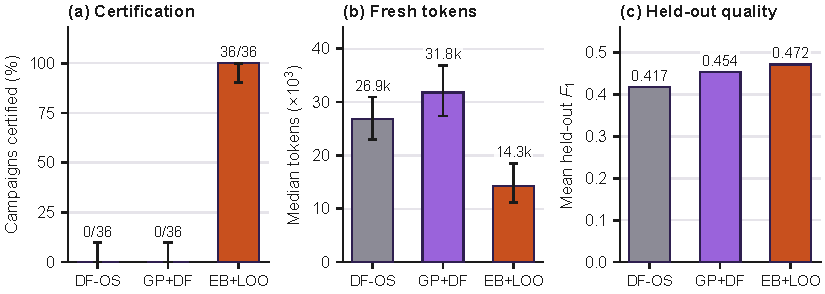
\includegraphics{figures/supp_live_workflow_validation.pdf}
\vspace{-12pt}
\caption{\textbf{Live agentic-workflow evaluation with fresh uncached Qwen3-0.6B inference.} Across $36$ campaigns and four domains: (a) certifications by the $60$-evaluation cap with $95\%$ Clopper--Pearson intervals, (b) median actual fresh inference tokens with interquartile ranges, and (c) held-out-task $F_1$ for formal DF-OS, GP-guided acquisition with DF stopping, and empirically calibrated EB+LOO stopping. Replotted from Table~\ref{tab:app-v11-live36}; only the first two methods have the stated distribution-free stopping regime.}
\label{fig:app-v11}
\end{figure}

\begin{table}[!htbp]
\caption{\textbf{Expanded uncached live \texttt{Qwen3-0.6B} + \texttt{Qwen3-Embedding-0.6B} WorFBench certification across $2$ workflow base configurations $\times 4$ paired seeds $=8$ independent live campaigns ($24$ fresh runs, $\varepsilon=.08, \delta=.10$, $140$-evaluation cap, strict 3-way disjoint split, prior calibrated solely on $D_{\mathrm{cal}}$, zero cached scores).}}
\label{tab:app-v10-live}
\uniformaligntable{0.93}{%
\begin{tabular}{@{}llrrrrrrr@{}}
\toprule
\textbf{Scope} & \textbf{Method} & \textbf{Runs} & \textbf{Live Cert.} & \textbf{Med.\ Evals} & \textbf{Med.\ Tokens} & \textbf{Infer (s)} & \textbf{Conic (s)} & \textbf{Unseen $D_{\mathrm{test}}$ $F_1$ (Reg.)} \\
\midrule
\multirow{3}{*}{All campaigns}
 & \textsc{Indep.\ OS} (DF) & $8$ & $0.0\%$ & $140.0^*$ & $71{,}372^*$ & $4{,}075.4$ & $0.000$ & $.4617$ ($.0000$) \\
 & \textsc{CD-Joint} (Calib.\ EB) & $8$ & $\mathbf{100.0\%}$ & $\mathbf{31.0}$ & $\mathbf{14{,}842}$ & $\mathbf{808.3}$ & $0.026$ & $.4617$ ($.0000$) \\
 & \textsc{CD-Joint} (Hybrid EB) & $8$ & $\mathbf{100.0\%}$ & $33.0$ & $16{,}772$ & $1{,}086.7$ & $0.032$ & $.4617$ ($.0000$) \\
\midrule
\multirow{3}{*}{Base $(1,0,0,0)$}
 & \textsc{Indep.\ OS} (DF) & $4$ & $0.0\%$ & $140.0^*$ & $65{,}046^*$ & $3{,}941.3$ & $0.000$ & $.4358$ ($.0000$) \\
 & \textsc{CD-Joint} (Calib.\ EB) & $4$ & $\mathbf{100.0\%}$ & $\mathbf{29.0}$ & $\mathbf{13{,}750}$ & $\mathbf{743.9}$ & $0.024$ & $.4358$ ($.0000$) \\
 & \textsc{CD-Joint} (Hybrid EB) & $4$ & $\mathbf{100.0\%}$ & $30.0$ & $14{,}262$ & $860.6$ & $0.029$ & $.4358$ ($.0000$) \\
\midrule
\multirow{3}{*}{Base $(0,0,0,0)$}
 & \textsc{Indep.\ OS} (DF) & $4$ & $0.0\%$ & $140.0^*$ & $76{,}717^*$ & $4{,}211.3$ & $0.000$ & $.4875$ ($.0000$) \\
 & \textsc{CD-Joint} (Calib.\ EB) & $4$ & $\mathbf{100.0\%}$ & $\mathbf{35.0}$ & $\mathbf{18{,}737}$ & $\mathbf{921.6}$ & $0.027$ & $.4875$ ($.0000$) \\
 & \textsc{CD-Joint} (Hybrid EB) & $4$ & $\mathbf{100.0\%}$ & $36.0$ & $20{,}085$ & $1{,}356.2$ & $0.040$ & $.4875$ ($.0000$) \\
\bottomrule
\end{tabular}%
}
\end{table}

\begin{table}[!htbp]
\caption{\textbf{WorFBench calibrated unseen-task generalization ($20$ campaigns $\times 10$ seeds $=200$ runs/method, $\varepsilon=.025, \delta=.05$) and fresh uncached live \texttt{Qwen3-0.6B} certification on strictly disjoint tasks ($\varepsilon=.08, \delta=.10$, $140$-evaluation cap, prior fit solely on $D_{\mathrm{cal}}$).} Offline panel reports median accounted tokens and untouched $D_{\mathrm{test}}$ $F_1$; live panel executes fresh local \texttt{Qwen3-0.6B} + \texttt{Qwen3-Embedding-0.6B} inference with zero caching and reports actual tokens, wall-clock inference versus conic oracle time, and $D_{\mathrm{test}}$ $F_1$.}
\label{tab:app-v8-worfbench}
\uniformaligntable{0.92}{%
\begin{tabular}{@{}llrrrrrr@{}}
\toprule
\textbf{Protocol} & \textbf{Method} & \textbf{Runs} & \textbf{Cert.\ (\%)} & \textbf{Err.} & \textbf{Med.\ Evals} & \textbf{Med.\ Tokens (Wall / Conic)} & \textbf{Unseen $D_{\mathrm{test}}$ $F_1$ (Reg.)} \\
\midrule
\multirow{5}{*}{Offline 20-camp.}
 & \textsc{Indep.\ OS} (DF) & $200$ & $100.0$ & $0$ & $1{,}897.5$ & $944$k ($1.00\times$) & $.5287$ ($.0000$) \\
 & \textsc{DF-CD Fallback} (DF) & $200$ & $100.0$ & $0$ & $1{,}897.5$ & $944$k ($1.00\times$) & $.5287$ ($.0000$) \\
 & \textsc{CD-Joint} (Nom.\ GP) & $200$ & $98.0$ & $0$ & $727.5$ & $366$k ($2.58\times$) & $.5187$ ($.0100$) \\
 & \textsc{CD-Joint} (Calib.\ EB) & $200$ & $98.5$ & $0$ & $\mathbf{318.0}$ & $\mathbf{165}$k ($\mathbf{5.73\times}$) & $.5189$ ($.0099$) \\
 & \textsc{CD-Joint} (Hybrid EB) & $200$ & $\mathbf{100.0}$ & $0$ & $327.0$ & $172$k ($5.48\times$) & $\mathbf{.5271}$ ($\mathbf{.0016}$) \\
\midrule
\multirow{4}{*}{Live \texttt{Qwen3-0.6B}}
 & \textsc{Indep.\ OS} (DF) & $2$ & $0.0$ & $0$ & $140.0^*$ & $65.5$k ($2{,}218$ s / $0.000$ s) & $.4358$ ($.0000$) \\
 & \textsc{CD-Joint} (Nom.\ GP) & $2$ & $\mathbf{100.0}$ & $0$ & $\mathbf{45.0}$ & $\mathbf{20.1}$k ($783$ s / $0.018$ s) & $.4358$ ($.0000$) \\
 & \textsc{CD-Joint} (Calib.\ EB) & $2$ & $\mathbf{100.0}$ & $0$ & $\mathbf{45.0}$ & $\mathbf{20.1}$k ($\mathbf{778}$ s / $0.018$ s) & $.4358$ ($.0000$) \\
 & \textsc{CD-Joint} (Hybrid EB) & $2$ & $\mathbf{100.0}$ & $0$ & $\mathbf{45.0}$ & $\mathbf{20.1}$k ($781$ s / $0.017$ s) & $.4358$ ($.0000$) \\
\bottomrule
\end{tabular}%
}
\par\vspace{2pt}\noindent
\parbox{\linewidth}{\scriptsize $^*$Uncertified at $140$-evaluation cap. All live runs use strictly fresh uncached inference ($46$--$72$ LLM generations + $52$--$74$ embedding calls per correlated run vs.\ $189$--$190$ / $192$--$194$ for OS); conic compute is $0.0023\%$ of total wall-clock time.}
\end{table}

\clearpage

\section{Extended Validation of Theoretical Results}
\label{app:group-extended}\label{app:validity-expanded}\label{app:unknown-expanded}

These experiments examine the dedicated likelihood-certified trackers, the consequences of unknown variances and misspecification, and certification along prescribed search trajectories. They are complementary to the primary CD-Joint acquisition comparison, not additional matched-model evidence for a universal acquisition advantage.

\subsection{Information-efficient likelihood tracking}

\begin{table}[!htbp]
\caption{\textbf{Decision-aware information tracking versus CD-Joint across small exact Gaussian instances ($80$ reps/cell, $\delta\in\{.10,.05,.005,10^{-4}\}$), medium overlapping DAGs ($16$ seeds/scale), and multi-answer tied optima ($48$ seeds).} Independent CVXPY primal QPs match $T_*^\varepsilon(\theta)$ to $\le 3.2\times10^{-10}$; zero false certificates occur across all $10{,}080$ runs.}
\label{tab:app-v8-tracking}
\uniformaligntable{0.92}{%
\begin{tabular}{@{}llrrrrrr@{}}
\toprule
\textbf{Regime / Instance} & \textbf{Metric / $\delta$} & \textbf{Info-Track} & \textbf{Hyb.\ CD$\to$Trk} & \textbf{CD-Joint} & \textbf{GP-UCB+J} & \textbf{Indep.\ OS} & \textbf{Trk / CD ms} \\
\midrule
Proxy ($M=5,d=3, T_*=1.11$) & Ratio $\delta=.10/.05/.005/10^{-4}$ & $\mathbf{8.07/6.50/4.02/3.03}$ & $10.1/7.87/5.09/3.64$ & $15.0/10.5/8.40/7.88$ & $240/193/134/118$ & $349/285/198/114$ & $39$ / $10$ \\
Gauss ($M=16,d=4, T_*=2.84$) & Ratio $\delta=.10/.05/.005/10^{-4}$ & $12.6/10.0/6.31/4.17$ & $13.7/10.8/6.68/4.37$ & $\mathbf{12.3/9.76/6.01/3.95}$ & $135/116/74.1/51.8$ & $66.0/45.3/22.9/18.4$ & $91$ / $32$ \\
Gauss ($M=32,d=6, T_*=10.38$) & Ratio $\delta=.10/.05/.005/10^{-4}$ & $18.3/13.7/8.50/5.55$ & $18.7/13.8/8.68/5.66$ & $\mathbf{16.7/13.0/7.90/5.30}$ & $73.2/57.4/35.3/22.7$ & $43.7/47.4/26.3/19.9$ & $1{,}825$ / $144$ \\
Gauss ($M=64,d=8, T_*=3.66$) & Ratio $\delta=.10/.05/.005/10^{-4}$ & $\mathbf{19.6/15.5}/9.34/\mathbf{5.87}$ & $22.0/17.0/10.2/6.39$ & $20.1/15.6/\mathbf{9.27}/5.87$ & $176/139/85.5/54.9$ & $150/134/94.0/51.2$ & $472$ / $120$ \\
\midrule
Medium ($M=128, d=8$) & Med.\ evals (cert.\ \%) & $\mathbf{285}$ ($100\%$) & $310$ ($100\%$) & $310$ ($100\%$) & $1{,}605$ ($93.8\%$) & $584$ ($93.8\%$) & $437$ / $137$ \\
Medium ($M=256, d=16$) & Med.\ evals (cert.\ \%) & $\mathbf{1{,}470}$ ($100\%$) & $1{,}660$ ($100\%$) & $1{,}515$ ($100\%$) & $3{,}900$ ($87.5\%$) & $1{,}561$ ($68.8\%$) & $2{,}277$ / $677$ \\
Medium ($M=512, d=32$) & Med.\ evals (cert.\ \%) & $4{,}770$ ($75.0\%$) & $5{,}130$ ($75.0\%$) & $3{,}765$ ($87.5\%$) & $6{,}000$ ($0.0\%$) & $\mathbf{1{,}535}$ ($87.5\%$) & $6{,}302$ / $1{,}852$ \\
\midrule
Multi-Answer Ties ($48$ reps) & Med.\ evals (easy act.\ \%) & $\mathbf{40.0}$ ($\mathbf{100\%}$) & $44.0$ ($\mathbf{100\%}$) & $87.5$ ($100\%$) & $68.0$ ($100\%$) & $3{,}500^*$ ($0\%$) & $3{,}213$ / $274$ \\
\bottomrule
\end{tabular}%
}
\end{table}

\begin{figure}[t]
\centering
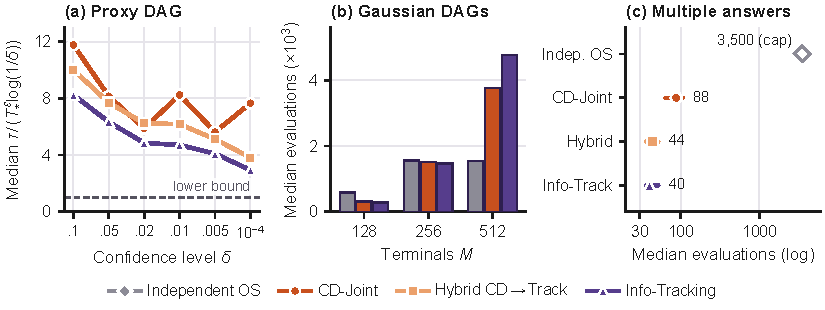
\includegraphics{figures/supp_information_tracking.pdf}
\vspace{-12pt}
\caption{\textbf{Information-efficient likelihood tracking compared with practical contrast acquisition.} (a) Proxy DAG normalized observation counts versus the characteristic-time bound at four confidence levels. (b) Observed median evaluations on medium Gaussian DAGs. (c) Multiple-correct-answer cohort (medians and interquartile ranges), with independent OS capped at $3{,}500$ evaluations (hollow marker). All values are replotted from Table~\ref{tab:app-v8-tracking}; these likelihood-certified trackers are distinct from CD-Joint.}
\label{fig:info-tracking}\label{fig:joint-phase}
\end{figure}

\subsection{Controlled calibration and bounded-residual robustness}

\begin{table}[!htbp]
\caption{\textbf{Complete calibration and misspecification grid across $\delta\in\{0.01, 0.05, 0.10\}$ and residual $\xi\in\{0, 0.02, 0.04, 0.08\}$ ($5{,}800$ replications).}}
\label{tab:app-e5}
\uniformaligntable{0.92}{%
\begin{tabular}{@{}lccrrrr@{}}
\toprule
\textbf{Condition} & $\delta$ / $\xi$ & \textbf{Method} & \textbf{Reps} & \textbf{Cert.\ (\%)} & \textbf{Err.\ (\%)} & \textbf{Med.\ Evals} \\
\midrule
C1: Valid Linear & $\delta=0.01/0.05/0.10$ & \textsc{Freq.\ Ellipsoid} & $200\times 3$ & $100/100/100$ & $0.0 / 0.0 / 0.0$ & $205 / 185 / 180$ \\
C1: Valid Linear & $\delta=0.01/0.05/0.10$ & \textsc{Bayes Posterior} & $200\times 3$ & $100/100/100$ & $0.0 / 2.0 / 10.0$ & $25 / 16 / 12$ \\
\midrule
C2: Valid GP Prior & $\delta=0.01/0.05/0.10$ & \textsc{Nominal Ellipsoid} & $200\times 3$ & $96/97/96.5$ & $0.0 / 0.0 / 0.0$ & $562 / 540 / 510$ \\
C2: Valid GP Prior & $\delta=0.01/0.05/0.10$ & \textsc{Bayes Posterior} & $200\times 3$ & $100/100/100$ & $0.5 / 2.5 / 7.0$ & $105 / 60 / 45$ \\
\midrule
C3: Misspec.\ GP & $\delta=0.01/0.05/0.10$ & \textsc{Nominal Ellipsoid} & $200\times 3$ & $99/97.5/98.5$ & $\mathbf{19.5 / 18.5 / 21.0}$ & $250 / 215 / 198$ \\
C3: Misspec.\ GP & $\delta=0.01/0.05/0.10$ & \textsc{Bayes Posterior} & $200\times 3$ & $100/100/100$ & $\mathbf{29.0 / 35.0 / 41.5}$ & $40 / 26 / 16$ \\
\midrule
C4: Residual $\xi$ & $\xi=0 / .02 / .04 / .08$ & \textsc{Unadjusted Ellip.} & $100\times 4$ & $100/100/98/100$ & $0 / 0 / 1 / \mathbf{11.0}$ & $152 / 420 / 720 / 232$ \\
C4: Residual $\xi$ & $\xi=0 / .02 / .04 / .08$ & \textsc{T3.3 Robust Ellip.} & $100\times 4$ & $100/0/0/0$ & $0 / 0 / 0 / 0$ & $152 / 3.5\text{k} / 3.5\text{k} / 3.5\text{k}$ \\
C4: Residual $\xi$ & $\xi=0 / .02 / .04 / .08$ & \textsc{Safe Hybrid} & $100\times 4$ & $100/0/0/0$ & $0 / 0 / 0 / 0$ & $172 / 3.5\text{k} / 3.5\text{k} / 3.5\text{k}$ \\
\bottomrule
\end{tabular}%
}
\end{table}

\begin{table}[!htbp]
\caption{\textbf{High-power controlled calibration cure and $(\xi,\varepsilon)$ feasibility frontier ($500$ replications/cell, $\delta=.05$).} Top block replicates the rough-true ($\ell=.45$) versus smooth-assumed ($\ell=3.0$) GP stress test. Bottom blocks map the bounded-residual sweep ($\xi\in\{0,.005,.01,.02,.04,.08\}$, cap $7{,}500$), showing \textsc{Smart Hybrid} capturing correlated speedups inside $2\xi<\varepsilon$ and falling back with $0/500$ errors once $2\xi\ge\varepsilon$.}
\label{tab:app-v8-calib}
\uniformaligntable{0.92}{%
\begin{tabular}{@{}lclrrrrr@{}}
\toprule
\textbf{Study} & $\varepsilon$ / $\xi$ & \textbf{Method} & \textbf{Cert.\ (\%)} & \textbf{Err.\ (/500)} & \textbf{CP95 Up.} & \textbf{Med.\ Evals} & \textbf{Mean Reg.} \\
\midrule
\multirow{3}{*}{Misspec.\ GP ($\ell=.45$ vs $3.0$)}
 & $.030$ / $0$ & \textsc{Posterior Nominal} & $100.0$ & $194$ ($38.8\%$) & $42.5\%$ & $27.0$ & $.0508$ \\
 & $.030$ / $0$ & \textsc{Ellipsoid Nominal} & $99.8$ & $133$ ($26.6\%$) & $30.1\%$ & $195.0$ & $.0299$ \\
 & $.030$ / $0$ & \textsc{Calibrated EB+LOO} & $99.2$ & $\mathbf{0}$ ($\mathbf{0.0\%}$) & $\mathbf{0.6\%}$ & $435.0$ & $.0002$ \\
\midrule
\multirow{6}{*}{$(\xi,\varepsilon)$ Frontier ($\varepsilon=.030$)}
 & $\xi=.000$ & \textsc{OS} / \textsc{Rob.} / \textsc{Hybrid} / \textsc{Nom.} & $100/100/100/100$ & $0/0/0/0$ & $0.6\%$ & $2{,}848/165/\mathbf{170}/105$ & $.0000$ \\
 & $\xi=.005$ & \textsc{OS} / \textsc{Rob.} / \textsc{Hybrid} / \textsc{Nom.} & $100/90.4/99.8/100$ & $0/0/0/0$ & $0.6\%$ & $3{,}065/358/\mathbf{420}/123$ & $.0000$ \\
 & $\xi=.010$ & \textsc{OS} / \textsc{Rob.} / \textsc{Hybrid} / \textsc{Nom.} & $100/3.0/98.2/100$ & $0/0/0/0$ & $0.6\%$ & $3{,}319/7{,}500/\mathbf{3{,}670}/150$ & $.0000$ \\
 & $\xi=.020^\dagger$ & \textsc{OS} / \textsc{Rob.} / \textsc{Hybrid} / \textsc{Nom.} & $100/0.0/100/100$ & $0/0/0/0$ & $0.6\%$ & $4{,}142/7{,}500/\mathbf{4{,}520}/240$ & $.0000$ \\
 & $\xi=.040^\dagger$ & \textsc{OS} / \textsc{Rob.} / \textsc{Hybrid} / \textsc{Nom.} & $100/0.0/99.2/100$ & $0/0/\mathbf{0}/6$ & $0.6\%$ & $4{,}192/7{,}500/\mathbf{4{,}590}/365$ & $.0001$ \\
 & $\xi=.080^\dagger$ & \textsc{OS} / \textsc{Rob.} / \textsc{Hybrid} / \textsc{Nom.} & $100/0.0/100/100$ & $0/0/\mathbf{0}/\mathbf{71}$ & $0.6\%$ & $3{,}478/7{,}500/\mathbf{3{,}793}/145$ & $.0001$ \\
\midrule
\multirow{4}{*}{$(\xi,\varepsilon)$ Frontier ($\varepsilon=.080$)}
 & $\xi=.000$ & \textsc{OS} / \textsc{Rob.} / \textsc{Hybrid} / \textsc{Nom.} & $100/100/100/100$ & $0/0/0/0$ & $0.6\%$ & $2{,}164/60/\mathbf{64}/40$ & $.0000$ \\
 & $\xi=.005$ & \textsc{OS} / \textsc{Rob.} / \textsc{Hybrid} / \textsc{Nom.} & $100/100/100/100$ & $0/0/0/0$ & $0.6\%$ & $2{,}263/95/\mathbf{95}/44$ & $.0001$ \\
 & $\xi=.010$ & \textsc{OS} / \textsc{Rob.} / \textsc{Hybrid} / \textsc{Nom.} & $100/69.4/92.0/100$ & $0/0/0/0$ & $0.6\%$ & $2{,}380/155/\mathbf{165}/48$ & $.0000$ \\
 & $\xi=.080^\dagger$ & \textsc{OS} / \textsc{Rob.} / \textsc{Hybrid} / \textsc{Nom.} & $100/0.0/100/100$ & $0/0/\mathbf{0}/12$ & $0.6\%$ & $2{,}310/7{,}500/\mathbf{2{,}535}/48$ & $.0003$ \\
\bottomrule
\multicolumn{8}{@{}l@{}}{\scriptsize $^\dagger$Rows with $2\xi\ge\varepsilon$ lie past the Theorem~\ref{thm:t3-misspec} robust bias floor; CP95 Up.\ and Mean Reg.\ columns correspond to \textsc{Hybrid}.}
\end{tabular}%
}
\end{table}

\begin{figure}[t]
\centering
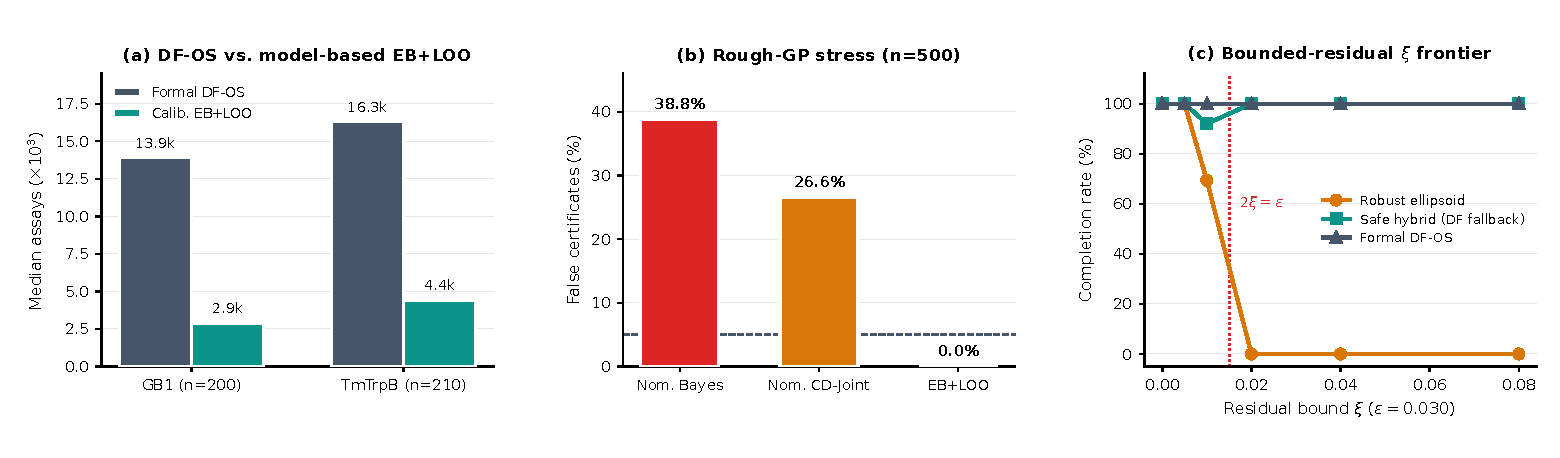
\includegraphics{figures/supp_protein_calibration_robustness.pdf}
\vspace{-12pt}
\caption{\textbf{Model-based speed and statistical robustness are distinct.} (a) Median retrospective protein assays using formal DF-OS versus calibrated empirical-Bayes (EB+LOO) stopping. (b) Observed incorrect-certification percentages under a rough true kernel and smoother assumed GP. (c) Completion rates of robust ellipsoidal and safe-hybrid policies across the bounded-residual $\xi$ frontier at $\varepsilon=.030$. Replotted from Tables~\ref{tab:app-v8-proteins} and~\ref{tab:app-v8-calib}; model-based gains do not establish formal coverage on measured proteins.}
\label{fig:real-world-calib}
\end{figure}

\subsection{Unknown-variance Gaussian tracking and heteroscedasticity}

Tables~\ref{tab:app-v9-ablation}--\ref{tab:app-v9-validity} and Figure~\ref{fig:app-v9-safety} report four paired empirical suites illustrating Sparse-KL performance and the deterministic solver-call accounting of Proposition~\ref{prop:v34-work}; the sharp-rate guarantee additionally requires the predictive and numerical contracts in Theorem~\ref{thm:v34-adaptive} ($15{,}376$ total runs). Throughout, \textsc{Dense-KL} denotes the square-refresh ($k^2$) all-action tracker, \textsc{Sparse-KL} denotes the sparse four-power ($4^k$) action-local tracker of Theorem~\ref{thm:v34-adaptive}, \textsc{Gated Sparse-KL} adds a predictable batch-activation gate that skips early low-SNR batches where expected profiling overhead exceeds batch information, and \textsc{Indep.\ Student-t OS} denotes Gaussian-exact (not distribution-free) per-terminal Student-$t$ Optimistic-Separation on identical paired observation tapes (\cref{eq:v34-student-t-box}).

\begin{figure}[!htbp]
\centering
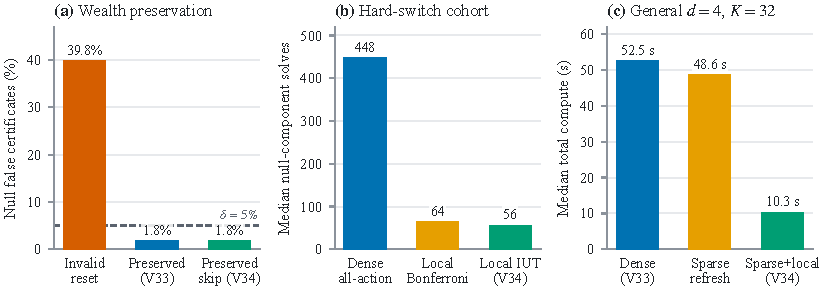
\includegraphics{figures/supp_eprocess_safety_and_compute.pdf}
\vspace{-12pt}
\caption{\textbf{Why predictable wealth and action-local tests matter.} (a) Null-boundary false-certificate percentages with legally preserved skipped wealth versus the invalid wealth-reset ablation ($n=500$). (b) Null-component solves in the hard-initial-action switch cohort ($K=8$), dense versus action-local intersection--union testing. (c) Total compute on a general $d=4,K=32$ case, dense versus sparse likelihood tracking. Values are reported in Tables~\ref{tab:app-v9-switching} and~\ref{tab:app-v9-ablation}; the reset policy is deliberately invalid.}
\label{fig:app-v9-safety}
\end{figure}

\begin{table}[!htbp]
\caption{\textbf{Full $2\times 2$ ablation of square versus sparse four-power refreshes and all-action versus action-local evidence on overlapping multi-action DAGs ($0$ false certificates across all $3{,}168$ runs; $100\%$ satisfaction of Proposition~\ref{prop:v34-work} call bounds).} Rank-2 cubic uses $24$ paired seeds/cell ($K\in\{4,16,64\}$, $\sigma=(.5,2.0)$); general $d=4$ B\&B uses $16$ paired seeds/cell ($K\in\{4,16,32\}$). Peak RAM is measured in isolated \texttt{tracemalloc} probes outside wall-clock timing.}
\label{tab:app-v9-ablation}
\uniformaligntable{0.92}{%
\begin{tabular}{@{}llrrrrrrrr@{}}
\toprule
\textbf{Track ($K, \delta$)} & \textbf{Method} & \textbf{Med.\ $N$} & \textbf{Des.\ Calls} & \textbf{Null Calls} & \textbf{Des.\ (ms)} & \textbf{Null (ms)} & \textbf{Tot.\ (ms)} & \textbf{RAM (KB)} \\
\midrule
\multirow{6}{*}{Rank-2 ($K=4, .01$)}
 & \textsc{Dense-KL} (sq., all) & $1{,}062.5$ & $16$ & $1{,}904$ & $40.1$ & $372.7$ & $424.6$ & $36.8$ \\
 & \textsc{Dense-KL+Sparse} ($4^k$, all) & $1{,}155.0$ & $8$ & $1{,}988$ & $23.4$ & $357.5$ & $385.2$ & --- \\
 & \textsc{Dense-KL+Local} (sq., loc.) & $891.0$ & $16$ & $427$ & $36.1$ & $103.3$ & $145.9$ & --- \\
 & \textsc{Sparse-KL} ($4^k$, loc.) & $1{,}012.0$ & $\mathbf{8}$ & $\mathbf{462}$ & $\mathbf{22.1}$ & $114.8$ & $\mathbf{143.2}$ & $\mathbf{24.7}$ \\
 & \textsc{Known-$\sigma$ Tracker} & $315.0$ & $47$ & $4{,}396$ & $2{,}173.6$ & $678.6$ & $2{,}862.3$ & --- \\
 & \textsc{Indep.\ Student-t OS} & $18{,}940.0$ & $0$ & $0$ & $0.0$ & $0.0$ & $1{,}072.1$ & --- \\
\midrule
\multirow{6}{*}{Rank-2 ($K=16, .01$)}
 & \textsc{Dense-KL} (sq., all) & $1{,}197.0$ & $80$ & $12{,}672$ & $61.4$ & $2{,}850.3$ & $2{,}919.6$ & $79.7$ \\
 & \textsc{Dense-KL+Sparse} ($4^k$, all) & $1{,}197.0$ & $32$ & $12{,}672$ & $33.8$ & $2{,}690.6$ & $2{,}745.7$ & --- \\
 & \textsc{Dense-KL+Local} (sq., loc.) & $1{,}038.0$ & $64$ & $737$ & $61.6$ & $185.5$ & $246.6$ & --- \\
 & \textsc{Sparse-KL} ($4^k$, loc.) & $\mathbf{1{,}012.0}$ & $\mathbf{32}$ & $\mathbf{726}$ & $34.8$ & $\mathbf{178.8}$ & $\mathbf{228.9}$ & $\mathbf{37.9}$ \\
 & \textsc{Known-$\sigma$ Tracker} & $315.0$ & $62$ & $6{,}908$ & $3{,}449.0$ & $1{,}048.5$ & $4{,}451.2$ & --- \\
 & \textsc{Indep.\ Student-t OS} & $18{,}940.0$ & $0$ & $0$ & $0.0$ & $0.0$ & $1{,}244.3$ & --- \\
\midrule
\multirow{6}{*}{Rank-2 ($K=64, .01$)}
 & \textsc{Dense-KL} (sq., all) & $1{,}239.0$ & $320$ & $163{,}520$ & $151.8$ & $33{,}862.1$ & $34{,}024.9$ & $722.0$ \\
 & \textsc{Dense-KL+Sparse} ($4^k$, all) & $1{,}239.0$ & $128$ & $163{,}520$ & $90.8$ & $32{,}818.3$ & $32{,}921.5$ & --- \\
 & \textsc{Dense-KL+Local} (sq., loc.) & $1{,}197.0$ & $320$ & $2{,}520$ & $153.6$ & $574.7$ & $768.4$ & --- \\
 & \textsc{Sparse-KL} ($4^k$, loc.) & $\mathbf{1{,}062.5}$ & $\mathbf{128}$ & $\mathbf{2{,}380}$ & $99.4$ & $\mathbf{554.0}$ & $\mathbf{674.7}$ & $\mathbf{170.2}$ \\
 & \textsc{Known-$\sigma$ Tracker} & $315.0$ & $169$ & $21{,}980$ & $15{,}585.0$ & $3{,}088.7$ & $18{,}406.0$ & --- \\
 & \textsc{Indep.\ Student-t OS} & $18{,}940.0$ & $0$ & $0$ & $0.0$ & $0.0$ & $2{,}496.7$ & --- \\
\midrule
\multirow{4}{*}{Rank-2 ($K=64, 10^{-4}$)}
 & \textsc{Dense-KL} (sq., all) & $1{,}449.0$ & $320$ & $174{,}720$ & $153.7$ & $32{,}965.0$ & $33{,}157.9$ & $722.0$ \\
 & \textsc{Dense-KL+Local} (sq., loc.) & $1{,}323.0$ & $320$ & $2{,}625$ & $156.1$ & $626.2$ & $797.9$ & --- \\
 & \textsc{Sparse-KL} ($4^k$, loc.) & $\mathbf{1{,}281.0}$ & $\mathbf{128}$ & $\mathbf{2{,}590}$ & $\mathbf{91.0}$ & $\mathbf{605.8}$ & $\mathbf{733.7}$ & $\mathbf{170.2}$ \\
 & \textsc{Indep.\ Student-t OS} & $23{,}216.0$ & $0$ & $0$ & $0.0$ & $0.0$ & $2{,}584.4$ & --- \\
\midrule
\multirow{5}{*}{Gen.\ $d=4$ ($K=32, .01$)}
 & \textsc{Dense-KL} (sq., all) & $805.0$ & $96$ & $6{,}080$ & $6{,}309.8$ & $45{,}114.1$ & $52{,}539.1$ & $93.7$ \\
 & \textsc{Dense-KL+Local} (sq., loc.) & $805.0$ & $96$ & $190$ & $6{,}121.4$ & $4{,}964.0$ & $11{,}258.4$ & --- \\
 & \textsc{Dense-KL+Sparse} ($4^k$, all) & $805.0$ & $64$ & $6{,}080$ & $5{,}412.9$ & $41{,}835.5$ & $48{,}619.2$ & --- \\
 & \textsc{Sparse-KL} ($4^k$, loc.) & $805.0$ & $\mathbf{64}$ & $\mathbf{190}$ & $\mathbf{5{,}267.9}$ & $\mathbf{4{,}815.6}$ & $\mathbf{10{,}274.6}$ & $\mathbf{93.4}$ \\
 & \textsc{Indep.\ Student-t OS} & $\mathbf{512.0}$ & $0$ & $0$ & $0.0$ & $0.0$ & $122.4$ & --- \\
\bottomrule
\end{tabular}%
}
\end{table}

\begin{table}[!htbp]
\caption{\textbf{Unknown heteroscedastic variance efficiency across $\sigma_x\in\{.25,.5,1,2,4\}$ ($60$ paired seeds/profile at $\delta=.05$) and asymptotic $\delta\in[10^{-8},.10]$ sweeps ($60$ seeds/cell on rank-2; $24$ seeds/cell on $d=3,m=4$ proxy DAG).} Ratios report $\mathbb E[\tau_\delta]/(C_*(\theta,\sigma)^{-1}\log(1/\delta))$ using the exact unknown-variance nuisance-KL limit $C_*$; empirical slope and intercept $\widehat D$ fit $\mathbb E[\tau_\delta]\approx\widehat D+\widehat s\log(1/\delta)$ (Theorem~\ref{thm:v34-adaptive}).}
\label{tab:app-v9-hetero}
\uniformaligntable{0.92}{%
\begin{tabular}{@{}llrrrrrr@{}}
\toprule
\textbf{Profile / Sweep} & \textbf{Method} & \textbf{$1/C_*$} & \textbf{Cert.\ (\%)} & \textbf{Err.} & \textbf{Mean $N$} & \textbf{Ratio vs.\ $1/C_*$} & \textbf{Emp.\ Slope / $\widehat D$} \\
\midrule
$\sigma=(.25,.25)$, $\delta=.05$ & \textsc{Sparse-KL} / \textsc{Known-$\sigma$} / \textsc{OS} & $1.5$ & $100/100/100$ & $0/0/0$ & $\mathbf{50.6}$ / $6.0$ / $685.3$ & $10.97$ / $1.30$ / $148.7$ & --- \\
$\sigma=(.50,2.0)$, $\delta=.05$ & \textsc{Sparse-KL} / \textsc{Known-$\sigma$} / \textsc{OS} & $13.3$ & $100/100/100$ & $0/0/0$ & $\mathbf{479.1}$ / $140.7$ / $11{,}036$ & $12.03$ / $3.53$ / $277.1$ & --- \\
$\sigma=(1.0,1.0)$, $\delta=.05$ & \textsc{Sparse-KL} / \textsc{Known-$\sigma$} / \textsc{OS} & $7.6$ & $100/100/100$ & $0/0/0$ & $\mathbf{200.7}$ / $72.4$ / $15{,}815$ & $8.81$ / $3.18$ / $694.0$ & --- \\
$\sigma=(.25,4.0)$, $\delta=.05$ & \textsc{Sparse-KL} / \textsc{Known-$\sigma$} / \textsc{OS} & $40.7$ & $100/100/100$ & $0/0/0$ & $\mathbf{2{,}365}$ / $480.9$ / $36{,}988$ & $19.40$ / $3.94$ / $303.4$ & --- \\
$\sigma=(4.0,.25)$, $\delta=.05$ & \textsc{Sparse-KL} / \textsc{Known-$\sigma$} / \textsc{OS} & $46.8$ & $100/100/41.7$ & $0/0/0$ & $\mathbf{2{,}849}$ / $542.5$ / $239{,}295^*$ & $20.33$ / $3.87$ / $1{,}708^*$ & --- \\
$\sigma=(4.0,4.0)$, $\delta=.05$ & \textsc{Sparse-KL} / \textsc{Known-$\sigma$} / \textsc{OS} & $101.8$ & $100/100/0.0$ & $0/0/0$ & $\mathbf{6{,}799}$ / $1{,}011$ / $250{,}000^*$ & $22.30$ / $3.32$ / $820^*$ & --- \\
\midrule
\multirow{3}{*}{$\sigma=(.25,4.0)$, $\delta\in[.1,10^{-8}]$}
 & \textsc{Sparse-KL-Vanilla} (unk.\ $\sigma$) & $40.7$ & $100$ & $0/360$ & $2{,}226\to 3{,}686$ & $23.76\to \mathbf{4.92}$ & $89.1$ ($2.19\times$) / $2{,}048$ \\
 & \textsc{Gated Sparse-KL} (pred.\ gate) & $40.7$ & $100$ & $0/360$ & $2{,}873\to 4{,}144$ & $30.65\to 5.53$ & $\mathbf{77.8}$ ($\mathbf{1.91\times}$) / $2{,}709$ \\
 & \textsc{Known-$\sigma$} / \textsc{Student OS} & $40.7$ & $100/83$ & $0/0$ & $1{,}161$ / $600\mathrm{k}^*$ ($10^{-8}$) & $1.55$ / $800.4^*$ & $45.3$ ($1.11\times$) / $327$ \\
\midrule
\multirow{3}{*}{$\sigma=(.5,2.0)$, $\delta\in[.1,10^{-8}]$}
 & \textsc{Sparse-KL-Vanilla} (unk.\ $\sigma$) & $13.3$ & $100$ & $0/360$ & $423\to \mathbf{981}$ & $13.80\to \mathbf{4.01}$ & $34.1$ ($2.57\times$) / $359$ \\
 & \textsc{Gated Sparse-KL} (pred.\ gate) & $13.3$ & $100$ & $0/360$ & $662\to 1{,}165$ & $21.64\to 4.76$ & $\mathbf{31.1}$ ($\mathbf{2.34\times}$) / $596$ \\
 & \textsc{Known-$\sigma$} / \textsc{Student OS} & $13.3$ & $100/83$ & $0/0$ & $339$ / $600\mathrm{k}^*$ ($10^{-8}$) & $1.38$ / $2{,}450^*$ & $13.4$ ($1.01\times$) / $91$ \\
\midrule
\multirow{3}{*}{Proxy $d=3,m=4$, $\delta\in[.1,10^{-5}]$}
 & \textsc{Sparse-KL-Vanilla} (unk.\ $\sigma$) & $28.5$ & $100$ & $0/120$ & $3{,}342\to \mathbf{4{,}263}$ & $50.96\to \mathbf{13.00}$ & $101.3$ ($3.56\times$) / $3{,}108$ \\
 & \textsc{Gated Sparse-KL} ($3.3\times$ faster) & $28.5$ & $100$ & $0/120$ & $3{,}476\to 4{,}407$ & $53.01\to 13.44$ & $100.5$ ($3.53\times$) / $3{,}244$ \\
 & \textsc{Known-$\sigma$} / \textsc{Student OS} & $28.5$ & $100/100$ & $0/0$ & $894$ / $17{,}352$ ($10^{-5}$) & $2.73$ / $52.92$ & $43.2$ ($1.52\times$) / $403$ \\
\midrule
\multirow{4}{*}{Sym.\ compass ($\delta=.05$, $n=60$)}
 & $\sigma=(.25,.25)$: \textsc{Sparse-KL} / \textsc{Nom.\ $\sigma{=}1$} / \textsc{OS} & --- & $100/100/100$ & $0/0/0$ & $46.5$ / $30.7$ / $22.1$ & --- & $0.0\%$ / $0.0\%$ err. \\
 & $\sigma=(.50,2.0)$: \textsc{Sparse-KL} / \textsc{Nom.\ $\sigma{=}1$} / \textsc{OS} & --- & $100/100/100$ & $0/3/0$ & $\mathbf{219.3}$ / $25.2$ / $532.4$ & --- & $\mathbf{0.0\%}$ / $5.0\%$ err. \\
 & $\sigma=(.25,4.0)$: \textsc{Sparse-KL} / \textsc{Nom.\ $\sigma{=}1$} / \textsc{OS} & --- & $100/100/100$ & $0/\mathbf{9}/0$ & $\mathbf{927.8}$ / $16.0$ / $1{,}788$ & --- & $\mathbf{0.0\%}$ / $\mathbf{15.0\%}$ err. \\
 & $\sigma=(4.0,4.0)$: \textsc{Sparse-KL} / \textsc{Nom.\ $\sigma{=}1$} / \textsc{OS} & --- & $100/100/100$ & $0/\mathbf{36}/0$ & $\mathbf{2{,}516}$ / $6.8$ / $9{,}684$ & --- & $\mathbf{0.0\%}$ / $\mathbf{60.0\%}$ err. \\
\bottomrule
\end{tabular}%
}
\end{table}

\begin{table}[!htbp]
\caption{\textbf{Multi-answer switching, intersection--union budgeting, and null-boundary safety audits ($\delta=.05$).} Top panel runs $200$ paired seeds per regime ($K=8$ shared-support DAG with $3$ $\varepsilon$-optimal actions, and $K=6$ identically tied actions); bottom panel runs $500$ replications each on exact null-boundary switching (Theorem~\ref{thm:v34-action-local}) and $17{,}500$ Behrens--Fisher bimodal batches \citep{drton2008}.}
\label{tab:app-v9-switching}
\uniformaligntable{0.92}{%
\begin{tabular}{@{}llrrrrrr@{}}
\toprule
\textbf{Study / Regime} & \textbf{Method} & \textbf{Runs} & \textbf{Cert.\ / Err.} & \textbf{Easiest $A_0$} & \textbf{Switches} & \textbf{Med.\ $N$} & \textbf{Null Calls / Viol.} \\
\midrule
\multirow{4}{*}{Hard init ($K=8$)}
 & \textsc{Dense-KL-All-Action} & $200$ & $100\%$ / $0$ & $100\%$ & $0.98$ & $91.0$ & $448$ calls \\
 & \textsc{Sparse-KL} (IUT) & $200$ & $100\%$ / $0$ & $100\%$ & $1.00$ & $\mathbf{91.0}$ & $\mathbf{56}$ calls ($8.0\times$) \\
 & \textsc{Sparse-KL-Bonferroni} ($K|J_a|$) & $200$ & $100\%$ / $0$ & $100\%$ & $1.00$ & $109.0$ & $64$ calls \\
 & \textsc{Sparse-KL-Student Hedge} ($\pi=.5$) & $200$ & $100\%$ / $0$ & $100\%$ & $1.00$ & $91.0$ & $56$ calls \\
\midrule
\multirow{4}{*}{Adv.\ early switch ($K=8$)}
 & \textsc{Dense-KL-All-Action} & $200$ & $100\%$ / $0$ & $100\%$ & $1.43$ & $\mathbf{248.0}$ & $896$ calls \\
 & \textsc{Sparse-KL} (IUT) & $200$ & $100\%$ / $0$ & $100\%$ & $1.38$ & $275.0$ & $\mathbf{120}$ calls ($7.5\times$) \\
 & \textsc{Sparse-KL-Bonferroni} ($K|J_a|$) & $200$ & $100\%$ / $0$ & $100\%$ & $1.38$ & $303.0$ & $128$ calls \\
 & \textsc{Sparse-KL-Student Hedge} ($\pi=.5$) & $200$ & $100\%$ / $0$ & $100\%$ & $1.38$ & $303.0$ & $128$ calls \\
\midrule
\multirow{4}{*}{Tied identical ($K=6$)}
 & \textsc{Dense-KL-All-Action} & $200$ & $100\%$ / $0$ & $100\%$ & $0.11$ & $173.0$ & $440$ calls \\
 & \textsc{Sparse-KL} (hysteresis) & $200$ & $100\%$ / $0$ & --- & $\mathbf{0.14}$ & $\mathbf{173.0}$ & $\mathbf{77}$ calls ($5.7\times$) \\
 & \textsc{Sparse-KL No-Hysteresis} & $200$ & $100\%$ / $0$ & --- & $1.00$ & $173.0$ & $61$ calls \\
 & \textsc{Sparse-KL-Bonferroni} ($K|J_a|$) & $200$ & $100\%$ / $0$ & --- & $0.14$ & $222.0$ & $88.5$ calls \\
\midrule
\multirow{3}{*}{Null-boundary reset ($\delta=5\%$)}
 & \textsc{Dense-KL Preserved All} & $500$ & $9/500$ ($\mathbf{1.8\%}$) & --- & $0$ resets & --- & valid ($\le 5\%$) \\
 & \textsc{Sparse-KL Preserved Skip} & $500$ & $9/500$ ($\mathbf{1.8\%}$) & --- & $0$ resets & --- & valid ($\le 5\%$) \\
 & \textsc{Neg.\ Ctrl.\ Wealth Reset} & $500$ & $199/500$ ($\mathbf{39.8\%}$) & --- & $28.8$ resets & --- & \textbf{violates $\delta$} ($8\times$) \\
\midrule
\multirow{3}{*}{Behrens--Fisher null ($17.5\mathrm{k}$ batches)}
 & \textsc{Certified Cubic} (rank-2) & $500$ & $0/500$ ($\mathbf{0.0\%}$) & --- & --- & --- & $\mathbf{0.0000}$ nats max viol. \\
 & \textsc{Certified B\&B} (quad.\ dual) & $500$ & $0/500$ ($\mathbf{0.0\%}$) & --- & --- & --- & $\mathbf{0.0000}$ nats max viol. \\
 & \textsc{Neg.\ Ctrl.\ Local SLSQP} & $500$ & $0/500$ ($0.0\%$) & --- & --- & --- & $\mathbf{+6.745}$ nats ($100$ viols.) \\
\bottomrule
\end{tabular}%
}
\end{table}

\begin{table}[!htbp]
\caption{\textbf{Cost of certified global validity across feature rank $d\in\{2,4,6\}$, action count $K\in\{4,16\}$, and log-enclosure tolerance $\zeta\in\{1.0, 0.1, 10^{-3}, 10^{-5}\}$ nats ($\delta=.05$, $1{,}488$ total runs, $100\%$ certification rate, $0$ false certificates).} Times report cold medians across paired seeds ($16$ seeds for $d\in\{2,4\}$, $8$ seeds for $d=6$); break-even $c_{\mathrm{eval}}^*$ (at $\zeta=.1$) is the per-evaluation cost (ms) above which certified tracking beats independent Student-$t$ OS in total wall-clock time ($0.0$ means strictly faster even at zero evaluation cost; --- means Student-$t$ OS uses fewer samples on that high-SNR moderate-$\delta$ instance).}
\label{tab:app-v9-validity}
\uniformaligntable{0.92}{%
\begin{tabular}{@{}llrrrrrrr@{}}
\toprule
\textbf{Instance} & \textbf{Solver} & \textbf{Med.\ $N$ ($.1$)} & \textbf{ms ($\zeta{=}1$)} & \textbf{ms ($\zeta{=}.1$)} & \textbf{ms ($\zeta{=}10^{-3}$)} & \textbf{ms ($\zeta{=}10^{-5}$)} & \textbf{Nodes ($10^{-5}$)} & \textbf{$c_{\mathrm{eval}}^*$ (ms)} \\
\midrule
\multirow{5}{*}{$d=2, K=16$}
 & \textsc{Exact Cubic} (rank-$2$) & $1{,}012$ & $\mathbf{194.6}$ & $\mathbf{188.6}$ & $\mathbf{192.9}$ & $\mathbf{195.8}$ & $2{,}529$ & $\mathbf{0.000}$ \\
 & \textsc{Cold B\&B} (certified) & $\mathbf{915}$ & $1{,}402$ & $2{,}630$ & $5{,}867$ & $19{,}154$ & $46{,}605$ & $0.096$ \\
 & \textsc{Hybrid QP+Screened} & $1{,}063$ & $1{,}472$ & $2{,}425$ & $6{,}177$ & $17{,}431$ & $43{,}878$ & $0.084$ \\
 & \textsc{Hybrid QP+Gated} & $1{,}323$ & $500.3$ & $601.8$ & $1{,}033$ & $3{,}519$ & $7{,}530$ & $\mathbf{0.000}$ \\
 & \textsc{Indep.\ Student-t OS} & $17{,}248$ & --- & $1{,}061$ & --- & --- & $0$ & ref. \\
\midrule
\multirow{4}{*}{$d=4, K=4$}
 & \textsc{Cold B\&B} (certified) & $\mathbf{315}$ & $2{,}920$ & $4{,}529$ & $10{,}053$ & $13{,}007$ & $34{,}722$ & $54.4$ \\
 & \textsc{Hybrid QP+Screened} & $\mathbf{315}$ & $\mathbf{2{,}324}$ & $3{,}500$ & $7{,}702$ & $10{,}046$ & $25{,}885$ & $\mathbf{41.9}$ \\
 & \textsc{Hybrid QP+Gated} & $491.5$ & $3{,}170$ & $\mathbf{3{,}360}$ & $\mathbf{4{,}643}$ & $\mathbf{5{,}201}$ & $\mathbf{7{,}969}$ & --- \\
 & \textsc{Indep.\ Student-t OS} & $397.5$ & --- & $41.3$ & --- & --- & $0$ & ref. \\
\midrule
\multirow{4}{*}{$d=4, K=16$}
 & \textsc{Cold B\&B} (certified) & $469$ & $11{,}192$ & $16{,}082$ & $33{,}994$ & $45{,}268$ & $122{,}083$ & --- \\
 & \textsc{Hybrid QP+Screened} & $514.5$ & $10{,}761$ & $14{,}055$ & $29{,}473$ & $39{,}339$ & $101{,}281$ & --- \\
 & \textsc{Hybrid QP+Gated} & $779.5$ & $\mathbf{6{,}075}$ & $\mathbf{5{,}923}$ & $\mathbf{8{,}117}$ & $\mathbf{9{,}593}$ & $\mathbf{18{,}128}$ & --- \\
 & \textsc{Indep.\ Student-t OS} & $\mathbf{375.5}$ & --- & $52.8$ & --- & --- & $0$ & ref. \\
\midrule
\multirow{4}{*}{$d=6, K=16$}
 & \textsc{Cold B\&B} (certified) & $2{,}393$ & $113.7\text{s}$ & $138.8\text{s}$ & $154.7\text{s}$ & $156.0\text{s}$ & $325{,}371$ & --- \\
 & \textsc{Hybrid QP+Screened} & $2{,}331$ & $101.3\text{s}$ & $122.4\text{s}$ & $140.8\text{s}$ & $147.2\text{s}$ & $293{,}196$ & --- \\
 & \textsc{Hybrid QP+Gated} & $2{,}393$ & $\mathbf{37.4\text{s}}$ & $\mathbf{32.2\text{s}}$ & $\mathbf{31.9\text{s}}$ & $\mathbf{32.0\text{s}}$ & $\mathbf{13{,}946}$ & --- \\
 & \textsc{Indep.\ Student-t OS} & $\mathbf{1{,}998.5}$ & --- & $0.30\text{s}$ & --- & --- & $0$ & ref. \\
\bottomrule
\end{tabular}%
}
\end{table}

Table~\ref{tab:app-v9-validity} clarifies the practical operating regime of certified unknown-variance profiling. First, tightening the log-enclosure tolerance $\zeta$ from $0.1$ down to $10^{-5}$ nats ($10^4\times$ tighter) produces no further reduction in stopping sample count on $d\in\{4,6\}$ ($469$ samples at $d=4,K=16$; $2{,}393$ samples at $d=6,K=16$) while increasing cold B\&B runtime up to $4.04\times$ ($11.2\to 45.3$ s at $d=4$), confirming that moderate $\zeta\in[0.05,0.1]$ nats captures essentially all statistical efficiency. Second, on rank-$2$ graphs the exact cubic solver runs in $189$--$196$ ms independent of $\zeta$---$97.8\times$ faster than cold B\&B at $\zeta=10^{-5}$ and faster than independent Student-$t$ OS even at zero evaluation cost ($c_{\mathrm{eval}}^*=0.0$ ms, $17.0\times$ fewer observations). Third, on general $d\in\{4,6\}$ graphs, pairing quadratic-dual screening with predictable batch activation (\textsc{Hybrid QP+Gated}) reduces B\&B branch nodes by $6.7\times$ ($d=4,K=16$) to $23.3\times$ ($d=6,K=16$, $325.4\text{k}\to 13.9\text{k}$) and total runtime by $4.7\times$--$4.9\times$ ($156.0\to 32.0$ s at $d=6,K=16$, with identical $2{,}393$ samples). Finally, the table documents a finite-$\delta$ limitation: on high-SNR $d\in\{4,6\}$ instances at $\delta=.05$, the $m$-nat variance-profiling baseline causes the unknown-variance tracker to use slightly more samples than rectangular Student-$t$ OS ($469$ versus $376$ at $d=4,K=16$; $2{,}393$ versus $1{,}999$ at $d=6,K=16$), whereas rank-$2$ overlap ($c_{\mathrm{eval}}^*=0.0$--$0.096$ ms) and moderate-$K$ $d=4$ graphs ($c_{\mathrm{eval}}^*=41.9$ ms) give the reported evaluation-cost break-even thresholds.

\begin{figure}[t]
\centering
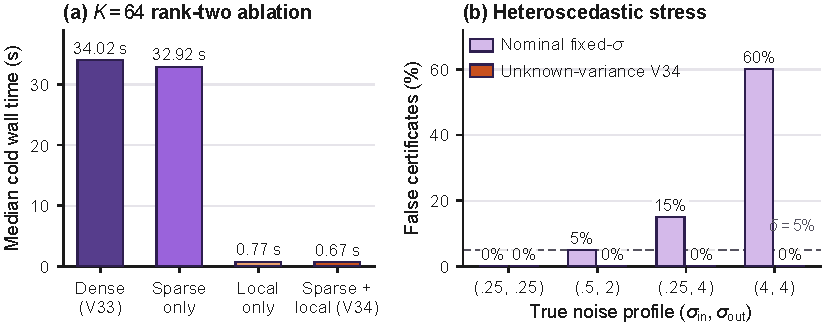
\includegraphics{figures/supp_sparse_variance_tracking.pdf}
\vspace{-12pt}
\caption{\textbf{Unknown-variance action-local evidence and heteroscedastic robustness.} (a) Recorded cold computation on the $K=64$ rank-two ablation: dense versus sparse action-local likelihood tracking. (b) Actual error rates across four true Gaussian noise-variance stress cases for a nominal fixed-variance acquisition/stop and the unknown-variance sparse likelihood test. Replotted from Tables~\ref{tab:app-v9-ablation} and~\ref{tab:app-v9-hetero}; the formal e-process guarantee requires the stated Gaussian and numerical contracts.}
\label{fig:v9-v34}
\end{figure}

\subsection{Cross-application validity and heteroscedastic controls}

The projected experiments satisfy the fixed-feature mean model by construction, whereas the raw measured landscapes test its misspecification boundary. The following cross-application summaries retain their original cohorts and estimands; the protein-specific and workflow-specific protocols are in Sections~\ref{app:group-proteins} and~\ref{app:group-workflows}.

\begin{table}[!htbp]
\caption{\textbf{Real-world heteroscedastic Sparse-KL bridge on measured GB1 ($10$ templates $\times 16$ seeds $=160$ runs/method, $M=21, K=6, d=3$, authentic Wu et al.\ sequencing read-count shot-noise spread $8.6\times$) and WorFBench ($8$ campaigns $\times 20$ seeds $=160$ runs/method, $M=14, K=4, d=4$, empirical task-score std spread $9.7\times$; $\delta=.05$, $40$k cap).} Compares exact fixed-feature projections (\emph{Projected}) against unprojected measured means (\emph{Raw, $\xi>0$}), isolating Sparse-KL's gains under fixed features from its residual-misspecification boundary, where full-rank \textsc{Calibrated EB+LOO} and \textsc{Student-$t$ OS} remain error-free.}
\label{tab:app-v10-real-v34}
\uniformaligntable{0.93}{%
\begin{tabular}{@{}llrrrrrr@{}}
\toprule
\textbf{Dataset / Track} & \textbf{Method} & \textbf{Cert.\ (\%)} & \textbf{Errors} & \textbf{Err.\ (\%)} & \textbf{Med.\ $N$} & \textbf{Mean Reg.} & \textbf{Med.\ ms} \\
\midrule
\multirow{5}{*}{GB1 Projected ($d{=}3$, $\xi{=}0$)}
 & \textsc{Sparse-KL (C++)} & $\mathbf{100.0}$ & $\mathbf{0/160}$ & $\mathbf{0.0}$ & $\mathbf{287.0}$ & $.0010$ & $375.8$ \\
 & \textsc{Gated Sparse-KL (C++)} & $96.9$ & $\mathbf{0/160}$ & $\mathbf{0.0}$ & $463.0$ & $.0010$ & $274.2$ \\
 & \textsc{CD-Joint (Nom.\ $\sigma$)} & $99.4$ & $2/160$ & $1.2$ & $65.0$ & $.0038$ & $30.4$ \\
 & \textsc{Calibrated EB+LOO} & $16.9$ & $0/160$ & $0.0$ & $12{,}000^*$ & $.0006$ & $1{,}238.5$ \\
 & \textsc{Indep.\ Student-t OS} & $6.2$ & $0/160$ & $0.0$ & $40{,}000^*$ & $.0273$ & $1{,}483.7$ \\
\midrule
\multirow{5}{*}{GB1 Raw Epist.\ ($\bar\xi{=}.423$)}
 & \textsc{Sparse-KL (C++)} & $90.0$ & $64/160$ & $40.0$ & $673.0$ & $.0708$ & $464.1$ \\
 & \textsc{Gated Sparse-KL (C++)} & $88.1$ & $62/160$ & $38.8$ & $774.0$ & $.0721$ & $314.9$ \\
 & \textsc{CD-Joint (Nom.\ $\sigma$)} & $100.0$ & $90/160$ & $56.2$ & $150.0$ & $.1072$ & $74.5$ \\
 & \textsc{Calibrated EB+LOO} & $\mathbf{82.5}$ & $\mathbf{0/160}$ & $\mathbf{0.0}$ & $\mathbf{3{,}870.0}$ & $\mathbf{.0017}$ & $467.9$ \\
 & \textsc{Indep.\ Student-t OS} & $16.2$ & $\mathbf{0/160}$ & $\mathbf{0.0}$ & $40{,}000^*$ & $.0110$ & $1{,}663.1$ \\
\midrule
\multirow{5}{*}{WorFBench Proj.\ ($d{=}4$, $\xi{=}0$)}
 & \textsc{Sparse-KL (C++)} & $100.0$ & $0/160$ & $0.0$ & $126.0$ & $.0000$ & $2{,}098.6$ \\
 & \textsc{Gated Sparse-KL (C++)} & $100.0$ & $0/160$ & $0.0$ & $210.0$ & $.0000$ & $2{,}014.6$ \\
 & \textsc{CD-Joint (Nom.\ $\sigma$)} & $100.0$ & $0/160$ & $0.0$ & $25.0$ & $.0000$ & $134.5$ \\
 & \textsc{Calibrated EB+LOO} & $100.0$ & $0/160$ & $0.0$ & $\mathbf{40.0}$ & $.0000$ & $39.7$ \\
 & \textsc{Indep.\ Student-t OS} & $100.0$ & $0/160$ & $0.0$ & $68.0$ & $.0000$ & $3.3$ \\
\midrule
\multirow{5}{*}{WorFBench Raw ($\bar\xi{=}.184$)}
 & \textsc{Sparse-KL (C++)} & $100.0$ & $0/160$ & $0.0$ & $126.0$ & $.0000$ & $2{,}099.9$ \\
 & \textsc{Gated Sparse-KL (C++)} & $100.0$ & $0/160$ & $0.0$ & $181.0$ & $.0000$ & $1{,}976.3$ \\
 & \textsc{CD-Joint (Nom.\ $\sigma$)} & $100.0$ & $0/160$ & $0.0$ & $20.0$ & $.0001$ & $82.1$ \\
 & \textsc{Calibrated EB+LOO} & $100.0$ & $0/160$ & $0.0$ & $\mathbf{40.0}$ & $.0000$ & $39.3$ \\
 & \textsc{Indep.\ Student-t OS} & $91.9$ & $0/160$ & $0.0$ & $65.5$ & $.0000$ & $3.0$ \\
\bottomrule
\end{tabular}%
}
\end{table}

\begin{table}[!htbp]
\caption{\textbf{Distribution-free certification on real-world configuration spaces.} GB1 uses $60$ trials per method and a $45$k cap; WorFBench uses $120$ and a $35$k cap. Counts are reported capped medians over each full cohort; $^*$ marks methods with censored runs.}
\label{tab:main-applications}\label{fig:real-world}
\centering\small
\begin{tabular}{@{}lrrrrr@{}}
\toprule
 & \multicolumn{2}{c}{GB1} & \multicolumn{3}{c}{WorFBench}\\
\cmidrule(lr){2-3}\cmidrule(lr){4-6}
Method & Certified & Assays & Certified & Evaluations & Tokens (M)\\
\midrule
Flat-LUCB & $60.0\%$ & $16{,}932^*$ & $59.2\%$ & $11{,}496^*$ & $6.39^*$\\
Flat-LUCB + Root Cert & $60.0\%$ & $16{,}930^*$ & $73.3\%$ & $8{,}486^*$ & $4.78^*$\\
Exact-Regret-DAG-LUCB & $96.7\%$ & $14{,}261^*$ & $100\%$ & $2{,}460$ & $1.44$\\
Optimistic-Separation & $100\%$ & $14{,}030$ & $100\%$ & $1{,}937$ & $0.95$\\
GP-Root-Info & $100\%$ & $13{,}688$ & --- & --- & ---\\
\bottomrule
\end{tabular}
\end{table}

\begin{table}[!htbp]
\centering
\caption{\textbf{Statistical validity in application-level comparisons.} GB1 ($n=200$) and TmTrpB ($n=210$) show median simulated assays under the corresponding $25$k cap. Live Qwen3 uses a separate $60$-evaluation cap and $\delta=.10$. The calibrated EB+LOO column is \emph{model-based}, whereas OS and strict EB\&DF use formal bounded-observation distribution-free stopping. The columns have different statistical guarantees; lower reported budgets alone do not establish an improvement at equal coverage.}
\label{tab:main-validity-contrast}
\small
\renewcommand{\arraystretch}{0.95}
\setlength{\tabcolsep}{4.2pt}
\begin{tabular}{@{}lrrr@{}}
\toprule
\textbf{Cohort} & \textbf{OS (formal DF)} & \textbf{Strict EB\&DF (formal DF)} & \textbf{EB+LOO (model-based)}\\
\midrule
GB1, $n=200$ & $13{,}890$ & $15{,}443$ & $\mathbf{2{,}895}$\\
TmTrpB, $n=210$ & $16{,}313$ & $16{,}810$ & $\mathbf{4{,}410}$\\
Live Qwen3, $n=36$ & $0/36$ cert. at cap & $0/36$ cert. at cap & $\mathbf{36/36}$ cert.\\
\bottomrule
\end{tabular}
\vspace{-8pt}
\end{table}
These studies evaluate initial-action decisions on measured protein landscapes and agentic workflows. Protein evaluations are retrospective simulated assays; workflow results include cached evaluations and separate uncached live executions. The tables distinguish outcome discovery, formal certification, and model-based stopping, and retain the corresponding observation and token budgets.

\begin{table}[t]
\caption{\textbf{Real-world validity ablation, heteroscedastic bridge, and $36$-campaign live LLM audit ($\delta=.05$; live $\delta=.10$).} GB1 ($200$) and TmTrpB ($210$, $\varepsilon=.015$) report $12$k/$25$k cert.\ rates, uncensored $25$k medians ($95\%$ paired bootstrap CIs vs.\ OS), errors (CP95 $\le 1.49\%/1.42\%$), and pointwise box coverage; bottom blocks show offline WorFBench ($200$), heteroscedastic Sparse-KL bridge ($160$), and $36$-campaign $4$-domain live \texttt{Qwen3-0.6B} (cap $60$; Table~\ref{tab:app-v11-live36}).}
\label{tab:bay-real}
\uniformaligntable{0.92}{%
\begin{tabular}{@{}lllrrr@{}}
\toprule
Dataset ($n$) & Method (Validity Tier) & Cert.\ (12k / 25k) & Median budget (CI) & Errors & Unseen / Diag. \\
\midrule
GB1 (200) & OS (Formal DF) & $5.5\%$ / $100\%$ & $13{,}890$ assays ($1.00\times$) & $0/200$ & pw.\ $100\%$ \\
 & Strict EB \& DF (Formal DF) & $4.0\%$ / $99.0\%$ & $15{,}443$ ($0.90\times$ $[.88,.94]$) & $0/200$ & pw.\ $100\%$ \\
 & Rob.\ $\xi{=}.005$ (Valid $|b|\le\xi$) & $55.5\%$ / $77.0\%$ & $10{,}620$ ($1.31\times$ $[1.14,2.17]$) & $0/200$ & pw.\ $100\%$ \\
 & Calib.\ EB+LOO (Model-based) & $91.0\%$ / $99.5\%$ & $\mathbf{2{,}895}$ ($\mathbf{4.80\times}$ $[3.83,5.61]$) & $0/200$ & pw.\ $91.5\%$ \\
\midrule
TmTrpB (210) & OS (Formal DF) & $0.0\%$ / $100\%$ & $16{,}313$ assays ($1.00\times$) & $0/210$ & pw.\ $100\%$ \\
 & Strict EB \& DF (Formal DF) & $0.0\%$ / $98.6\%$ & $16{,}810$ ($0.97\times$ $[.96,.98]$) & $0/210$ & pw.\ $100\%$ \\
 & Rob.\ $\xi{=}.005$ (Valid $|b|\le\xi$) & $26.2\%$ / $60.5\%$ & $15{,}360$ ($1.06\times$ $[1.02,1.09]$) & $0/210$ & pw.\ $100\%$ \\
 & Calib.\ EB+LOO (Model-based) & $85.7\%$ / $100\%$ & $\mathbf{4{,}410}$ ($\mathbf{3.70\times}$ $[3.37,4.35]$) & $0/210$ & pw.\ $82.9\%$ \\
\midrule
WorFBench (200) & OS (DF) / EB (Model-based) & $100\%$ / $98.5\%$ & $944$k / $\mathbf{165}$k tok. & $0/200$ / $0/200$ & $F_1=.529/.519$ \\
GB1 Het.\ Proj.\ (160) & \textsc{Sparse-KL (C++)} / \textsc{Stud.\ OS} & $\mathbf{100\%}$ / $6.2\%$ & $\mathbf{287}$ / $40\mathrm{k}^*$ assays & $0/160$ / $0/160$ & reg.\ $.0010/.0273$ \\
GB1 Het.\ Raw (160) & \textsc{Sparse-KL} / \textsc{Calib.\ EB} (Mod.) & $90.0\%$ / $82.5\%$ & $673$ / $\mathbf{3{,}870}$ assays & $64/160$ / $\mathbf{0/160}$ & $\bar\xi=.423$ \\
\midrule
Live \texttt{Qwen3} (36/m) & OS (Formal DF, 4 doms) & $0/36$ ($0.0\%$) & $26.9$k$^*$ tok.\ ($60^*$ ev.) & --- & reg.\ $.0671$ \\
 & EB acq $+$ DF stop (Formal DF) & $0/36$ ($0.0\%$) & $31.8$k$^*$ tok.\ ($60^*$ ev.) & --- & reg.\ $.0301$ \\
 & Calib.\ EB+LOO (Model-based) & $\mathbf{36/36}$ ($\mathbf{100\%}$) & $\mathbf{14.3\text{k}}$ tok.\ ($\mathbf{24.0}$ ev.) & --- & reg.\ $\mathbf{.0126}$ \\
\bottomrule
\end{tabular}%
}
\end{table}

\subsection{Passive UCT/PUCT evaluation protocols and certification horizons}
\label{sec:backup-experiments}\label{sec:primary-results}

\subsubsection{Primary online UCT evaluation}
\label{app:ta-data}

\paragraph{Experimental protocol and timing methodology.}

The primary evaluation (Section~\ref{sec:primary-results}, Table~\ref{tab:uct-backup-cert}) crossed the four exact-coupled confidence monitors (\emph{Eager}, \emph{Selective}, \emph{Flat}, and \emph{Covers}) with 16 benchmark configurations across eight paired pseudorandom seeds ($421001$--$421008$) and two counterbalanced timing repetitions per seed, totaling $1{,}024$ cold runs. Alongside the two-exit and one-exit dominated funnels of Theorem~\ref{thm:selective-separation}, the suite includes the winning-fanout control (where the high-fan-in paths lead to the optimal terminal), the fixed-gap ($g = 0.08$) one-exit funnel, the Bernoulli noisy one-exit funnel, the wide common-core family ($r \in \{8, 16, 32\}$), and two external transposition controls: a 6-feature Bernoulli subset lattice and a width-32, depth-6 shared merge network (both evaluated at tolerance $\epsilon = 0.08$). Root action orderings are shuffled once per seed and held identical across all four monitors.

To eliminate ordering bias, each seed block was executed in randomized method order and immediately repeated in reverse method order. Every timed run constructs its own TA-UCT allocator, terminal-local reward stream, confidence monitor, and auxiliary heap or cover structures from scratch inside the wall-clock timer before drawing its first rollout. Runs are capped at $2000\text{ ms}$ and $200{,}000$ rollouts, and restricted mean certification times assign the full $2000\text{ ms}$ cap to any run that does not certify before the cutoff. When a monitor certifies an $\epsilon$-optimal root action, the timer includes full deallocation and state release.

For anytime decision evaluation at fixed wall-clock deadlines ($1, 10, 100, 500$, and $2000\text{ ms}$), we record the most recent root recommendation published prior to each deadline (defaulting to root action $0$ if no rollout has completed before the deadline, as occurs when upfront support compilation exceeds $1\text{ ms}$ or $10\text{ ms}$). All four monitors memoize the most recent root confidence query whenever the updated terminal interval is unchanged.

\paragraph{Simple regret and finite-horizon tradeoffs.}

Tables~\ref{tab:ta-regret-1ms} and~\ref{tab:ta-regret-10ms} report the mean anytime simple regret across all 16 configurations at the $1\text{ ms}$ and $10\text{ ms}$ deadlines (complementing the certification time and operation counts in Table~\ref{tab:uct-backup-cert}). By the $100\text{ ms}$ deadline, mean simple regret reaches $0.000$ across every configuration and monitor except \emph{One-Exit Funnel ($64$)} under \emph{Covers} ($0.012$) and \emph{Feature Lattice ($6$)} under \emph{Flat} ($0.003$) and \emph{Covers} ($0.005$); by $500\text{ ms}$ and $2000\text{ ms}$, every cell is identically $0.000$.

Three structural patterns stand out. First, on \emph{Common Core} ($r = 32$), \emph{Flat} remains blocked inside its $\Omega(r^3)$ support-materialization loop beyond $10\text{ ms}$, incurring a mean simple regret of $1.000$ at both $1\text{ ms}$ and $10\text{ ms}$, whereas the graph monitors and \emph{Covers} execute rollouts much earlier and reach $0.000$ simple regret well before $100\text{ ms}$. Second, on the \emph{Feature Lattice} ($k=6$) and \emph{Shared Merge} ($W=32$) benchmarks, overlapping stochastic supports prevent formal $\epsilon$-certification within $2000\text{ ms}$ (Table~\ref{tab:uct-backup-cert}), yet TA-UCT still identifies an optimal root action on every seed by $100\text{ ms}$ on \emph{Shared Merge} and by $500\text{ ms}$ on \emph{Feature Lattice}. Third, in the stopping-horizon intervention of \cref{tab:uct-backup-gap} (Section~\ref{subsec:stopping-horizon-intervention}), narrowing the rival gap $g$ from $0.200$ to $0.075$ and $0.035$ extends the stopping horizon from $3{,}025$ to $36{,}821$ rollouts while holding branch retirement fixed at $t_{\mathrm{cut}}=1{,}024$, shifting the selective-to-eager work ratio from $1.218$ down to $0.933$.

\begin{table}[!t]
\caption{\textbf{Stopping-horizon intervention on the width-256 two-exit funnel ($192$ coupled runs).} Narrowing $g \in \{0.20, 0.075, 0.035\}$ at fixed retirement step $t_{\mathrm{cut}} = 1{,}024$ isolates post-cutoff UCT revisits.}
\label{tab:uct-backup-gap}
\uniformaligntable{0.92}{%
\begin{tabular}{@{}rrrrrrr@{}}
\toprule
\textbf{Rival Gap $g$} & \textbf{Mean $\tau$} & \textbf{Post-Cut Vis.} & \textbf{Msg.\ Ratio} & \textbf{Work Ratio} & \textbf{Eager (ms)} & \textbf{Selective (ms)} \\
\midrule
$0.200$ &  $3{,}025$ &  $2.6$ & $0.900$ & $1.218$ & $104.1$ & $143.5$ \\
$0.075$ & $14{,}666$ & $19.6$ & $0.875$ & $\mathbf{0.943}$ & $294.7$ & $317.3$ \\
$0.035$ & $36{,}821$ & $95.1$ & $\mathbf{0.858}$ & $\mathbf{0.933}$ & $579.1$ & $599.6$ \\
\bottomrule
\end{tabular}%
}
\end{table}

\begin{table}[!t]
\caption{\textbf{Mean anytime simple regret at the $1\text{ ms}$ wall-clock deadline across the $1{,}024$-run coupled UCT evaluation.} Upfront $\Omega(r^3)$ table construction blocks rollout execution in \emph{Flat} on \emph{Common Core}.}
\label{tab:ta-regret-early}\label{tab:ta-regret-1ms}
\uniformaligntable{0.92}{%
\begin{tabular}{@{}lrrrrr@{}}
\toprule
\textbf{Benchmark Family} & \textbf{Size} & \textbf{Eager} & \textbf{Selective} & \textbf{Flat} & \textbf{Covers} \\
\midrule
Two-Exit Funnel & $16$ & $0.000$ & $0.000$ & $0.000$ & $0.000$ \\
Two-Exit Funnel & $64$ & $0.012$ & $0.000$ & $0.000$ & $0.000$ \\
Two-Exit Funnel & $256$ & $0.113$ & $0.113$ & $0.000$ & $0.057$ \\
Two-Exit Funnel & $1024$ & $0.108$ & $0.108$ & $0.108$ & $0.108$ \\
One-Exit Funnel & $64$ & $0.000$ & $0.012$ & $0.000$ & $0.024$ \\
One-Exit Funnel & $256$ & $0.086$ & $0.129$ & $0.011$ & $0.022$ \\
Winning Fanout & $64$ & $0.000$ & $0.000$ & $0.000$ & $0.000$ \\
Winning Fanout & $256$ & $0.096$ & $0.129$ & $0.011$ & $0.011$ \\
Fixed-Gap Funnel & $64$ & $0.000$ & $0.000$ & $0.000$ & $0.000$ \\
Fixed-Gap Funnel & $256$ & $0.094$ & $0.100$ & $0.000$ & $0.037$ \\
Noisy Funnel & $256$ & $0.129$ & $0.129$ & $0.053$ & $0.098$ \\
Common Core & $8$ & $0.062$ & $0.000$ & $0.875$ & $0.062$ \\
Common Core & $16$ & $0.875$ & $0.875$ & $0.875$ & $0.875$ \\
Common Core & $32$ & $1.000$ & $1.000$ & $1.000$ & $1.000$ \\
Feature Lattice & $6$ & $0.003$ & $0.000$ & $0.005$ & $0.000$ \\
Shared Merge & $32$ & $0.047$ & $0.062$ & $0.125$ & $0.141$ \\
\bottomrule
\end{tabular}%
}
\end{table}

\begin{table}[!t]
\caption{\textbf{Mean anytime simple regret at the $10\text{ ms}$ wall-clock deadline across the $1{,}024$-run coupled UCT evaluation.} At $500\text{ ms}$ and $2000\text{ ms}$, mean simple regret equals $0.000$ for all families and monitors.}
\label{tab:ta-regret-late}\label{tab:ta-regret-10ms}
\uniformaligntable{0.92}{%
\begin{tabular}{@{}lrrrrr@{}}
\toprule
\textbf{Benchmark Family} & \textbf{Size} & \textbf{Eager} & \textbf{Selective} & \textbf{Flat} & \textbf{Covers} \\
\midrule
Two-Exit Funnel & $16\text{--}1024$ & $0.000$ & $0.000$ & $0.000$ & $0.000$ \\
One-Exit Funnel & $64$ & $0.000$ & $0.000$ & $0.000$ & $0.012$ \\
One-Exit Funnel & $256$ & $0.000$ & $0.000$ & $0.000$ & $0.000$ \\
Winning \& Fixed Funnels & $64, 256$ & $0.000$ & $0.000$ & $0.000$ & $0.000$ \\
Noisy Funnel & $256$ & $0.033$ & $0.022$ & $0.000$ & $0.000$ \\
Common Core & $8$ & $0.000$ & $0.000$ & $0.000$ & $0.000$ \\
Common Core & $16$ & $0.000$ & $0.000$ & $0.125$ & $0.000$ \\
Common Core & $32$ & $0.562$ & $0.938$ & $1.000$ & $0.500$ \\
Feature Lattice & $6$ & $0.005$ & $0.008$ & $0.005$ & $0.008$ \\
Shared Merge & $32$ & $0.141$ & $0.141$ & $0.062$ & $0.047$ \\
\bottomrule
\end{tabular}%
}
\end{table}

\subsubsection{Selective pruning and certification horizons}
\label{sec:backup-protocol}
\label{sec:backup-pruning-results}
\label{sec:backup-gap-intervention}
\label{subsec:stopping-horizon-intervention}
\label{sec:strong-compiler-results}
\label{sec:frontier-experiments}

In the $1{,}024$-run coupled UCT benchmark (\cref{tab:uct-backup-cert}), permanent edge retirement saves wall-clock time only when dominated branches detach early relative to the overall certification horizon $\tau$. On the baseline two-exit funnel ($m=256$), \emph{Graph-Selective} retires $74.8\%$ of edges at $t_{\mathrm{cut}}=1{,}466$, but certification finishes at $\tau=1{,}599$ after an average of $0.4$ post-cut revisits, leaving a $1.235\times$ work overhead. Extending the stopping horizon on the fixed-gap funnel ($\tau=5{,}380$) cuts selective work by $28.8\%$ ($143.2\text{ ms}$ versus $164.4\text{ ms}$). Similarly, on \emph{Sparse Catalog} ($k=4$, \cref{tab:uct-frontier-time}), \emph{Graph-Selective} retires $94.1\%$ of incidences yet performs $1.4\%$ more scalar operations than \emph{Graph-Eager} because dominance occurs near termination, whereas on \emph{Common Core} ($r=32$), \emph{Flat Supports} stalls in $\Omega(r^3)$ initialization ($70.4\text{ ms}$ versus $30.3\text{ ms}$ for \emph{Graph-Eager}).

\begin{table}[!t]
\caption{\textbf{Coupled UCT marginal-certification benchmark ($1{,}024$ runs; $16$ coupled runs per row, $2.0\text{ s}$ cap).} \emph{Sel./Eag.} is the selective-to-eager scalar work ratio; \emph{Cut} gives the final retired-edge fraction.}
\label{tab:uct-backup-cert}
\uniformaligntable{0.92}{%
\begin{tabular}{@{}lrrrrrrr@{}}
\toprule
\textbf{Benchmark Graph} & \textbf{Eager (ms)} & \textbf{Select.\ (ms)} & \textbf{Flat (ms)} & \textbf{Covers (ms)} & \textbf{Mean $\tau$} & \textbf{Sel./Eag.} & \textbf{Cut} \\
\midrule
Two-exit funnel ($16$)   &   $15.0$ &   $17.6$ &  $15.0$ &  $\mathbf{13.4}$ &  $1{,}185$ & $1.092$ & $0.73$ \\
Two-exit funnel ($64$)   &   $23.6$ &   $27.7$ &  $16.6$ &  $\mathbf{14.7}$ &  $1{,}327$ & $1.166$ & $0.74$ \\
Two-exit funnel ($256$)  &   $60.3$ &   $79.4$ &  $22.1$ &  $\mathbf{20.4}$ &  $1{,}599$ & $1.235$ & $0.75$ \\
Two-exit funnel ($1024$) &  $189.9$ &  $261.0$ &  $26.7$ &  $\mathbf{25.1}$ &  $1{,}931$ & $1.268$ & $0.75$ \\
\midrule
One-exit funnel ($64$)   &   $34.0$ &   $34.9$ &  $\mathbf{16.8}$ &  $25.7$ &  $1{,}285$ & $\mathbf{0.987}$ & $0.96$ \\
One-exit funnel ($256$)  &   $97.2$ &   $95.3$ &  $22.0$ &  $\mathbf{19.4}$ &  $1{,}550$ & $\mathbf{0.904}$ & $0.99$ \\
Winning fanout ($64$)    &  $338.7$ &  $458.5$ &  $28.9$ &  $\mathbf{24.5}$ &  $1{,}285$ & $1.242$ & $0.00$ \\
Winning fanout ($256$)   & $1592.7$ & $1999.5^*$ & $41.8$ & $\mathbf{34.5}$ &  $1{,}550$ & $1.251$ & $0.00$ \\
\midrule
Fixed-gap funnel ($64$)  &   $94.4$ &   $87.2$ &  $74.4$ &  $\mathbf{71.7}$ &  $5{,}380$ & $\mathbf{0.848}$ & $0.96$ \\
Fixed-gap funnel ($256$) &  $164.4$ &  $143.2$ &  $72.8$ &  $\mathbf{63.0}$ &  $5{,}380$ & $\mathbf{0.712}$ & $0.99$ \\
Stochastic funnel ($256$)&   $48.5$ &   $52.3$ &  $15.3$ &  $\mathbf{12.7}$ &  $1{,}368$ & $1.001$ & $0.75$ \\
\midrule
Common core ($r{=}8$)    &    $5.8$ &    $\mathbf{5.7}$ &   $6.8$ &   $8.4$ &    $356$ & $1.026$ & $0.00$ \\
Common core ($r{=}16$)   &   $11.5$ &   $\mathbf{11.0}$ &  $16.9$ &  $18.8$ &    $502$ & $1.031$ & $0.00$ \\
Common core ($r{=}32$)   &   $\mathbf{30.3}$ &   $31.5$ &  $70.4$ &  $46.9$ &    $793$ & $1.038$ & $0.00$ \\
\midrule
Subset lattice ($d{=}6$) & $1080.9$ & $1191.2$ & $\mathbf{847.7}$ & $866.1$ & $39{,}960$ & $1.073$ & $0.58$ \\
Merge DAG ($W{=}32$)     & $2000^*$ & $2000^*$ & $2000^*$ & $2000^*$ & --- & --- & --- \\
\bottomrule
\end{tabular}%
}
\end{table}

\subsubsection{Transfer to fixed-prior and noisy recursive PUCT}
\label{sec:puct-experiments}

Across $1{,}248$ cold Python runs (\cref{tab:puct-summary}), deterministic Root-PUCT ($\alpha=1/4$, \cref{thm:puct-main}) tightens terminal endpoints on $99.7\%$--$100\%$ of visits, allowing \emph{Decision-Selective} to cut scalar work to $0.202\times$ and Python runtime by $3.87\times$ at $m=1024$ ($1{,}223.0\text{ ms}$ versus $4{,}730.1\text{ ms}$ for \emph{Graph-Eager}), and certify all runs at $m=2048$ where \emph{Graph-Eager} reaches the $5.5\text{ s}$ cap. Under noisy Recursive-PUCT (\cref{thm:puct-noisy-main}), running intersections tighten endpoints on $11.7\%$--$14.0\%$ of visits on funnels, so selective pruning improves over eager propagation primarily when misleading priors route substantial traffic into dominated high-fan-in subgraphs ($0.594\times$ work ratio).

\begin{table}[!t]
\caption{\textbf{Python Root-PUCT scaling and noisy Recursive-PUCT prior sensitivity ($1{,}248$ cold runs; paired work ratios and median certification times in ms).}}
\label{tab:puct-summary}
\uniformaligntable{0.92}{%
\begin{tabular}{@{}llrrrrr@{}}
\toprule
\textbf{Regime / Graph} & \textbf{Policy / Prior} & \textbf{Med.\ $\tau$} & \textbf{Dec./Eag.\ Work} & \textbf{Eager (ms)} & \textbf{Dec.\ (ms)} & \textbf{Dual (ms)} \\
\midrule
Root-PUCT ($m{=}64$)   & Root ($\lambda{=}1$) & $10{,}534$ & $0.628$ & $232.2$  & $172.7$  & $\mathbf{134.4}$ \\
Root-PUCT ($m{=}256$)  & Root ($\lambda{=}1$) & $23{,}320$ & $0.374$ & $915.2$  & $422.4$  & $\mathbf{292.2}$ \\
Root-PUCT ($m{=}1024$) & Root ($\lambda{=}1$) & $51{,}316$ & $\mathbf{0.202}$ & $4730.1$ & $1223.0$ & $\mathbf{647.5}$ \\
Root-PUCT ($m{=}2048$) & Root ($\lambda{=}1$) & $75{,}984$ & $\mathbf{0.315}^*$ & $5500^*$ & $2061.4$ & $\mathbf{941.9}$ \\
\midrule
Noisy Funnel ($256$) & Rec.\ Informative & $43{,}588$ & $0.963$ & $641.5$ & $656.6$ & $\mathbf{611.4}$ \\
Noisy Funnel ($256$) & Rec.\ Uniform     & $27{,}336$ & $1.021$ & $231.8$ & $246.5$ & $\mathbf{173.9}$ \\
Noisy Funnel ($256$) & Rec.\ Misleading  & $48{,}448$ & $\mathbf{0.594}$ & $773.3$ & $686.1$ & $\mathbf{649.7}$ \\
\midrule
Noisy Parity ($r{=}16$) & Rec.\ Uniform    & $356$ & $1.047$ & $\mathbf{11.4}$ & $12.1$ & $36.5$ \\
Noisy Parity ($r{=}16$) & Rec.\ Misleading & $370$ & $1.046$ & $\mathbf{12.7}$ & $13.1$ & $37.5$ \\
\bottomrule
\end{tabular}%
}
\end{table}

\subsubsection{SameGame lookahead}
\label{sec:samegame-selector-experiments}

Under conservative $[0,1]$ Hoeffding boxes ($696$ cold runs in \cref{tab:samegame-selector}), exact regret cuts median stopping rollouts on standard $15\times 15$ depth-$4$ endgames by $6.0\times$ ($\tau_{\mathrm{exact}}/\tau_{\mathrm{conv}}=0.167$) and halves mean runtime from $804.8\text{ ms}$ ($14/40$ certified) to $390.9\text{ ms}$ ($26/40$ certified), providing the baseline against which Empirical Bernstein boxes (\cref{tab:app-emp-bernstein-lucb}) achieve $100\%$ completion. Across $512$ exact-regret representation runs sharing identical $\tau_{\mathrm{exact}}$ (\cref{tab:app-repr-selector}), \emph{Direct-Graph-Regret} beats \emph{Charged Dual Covers} by $1.57\times$ on \emph{Parity Grid} ($r=32$), whereas \emph{Charged Dual Covers} wins on windows, common cores, and overlap DAGs, and our pre-run fragmentation selector (\emph{Paid-Selector}) tracks the winning representation across all families.

\begin{table}[!t]
\caption{\textbf{Natural SameGame lookahead DAGs under passive TA-UCT and Hoeffding boxes ($696$ runs, $1.0\text{ s}$ cap).}}
\label{tab:samegame-selector}
\uniformaligntable{0.92}{%
\begin{tabular}{@{}lrrrrrr@{}}
\toprule
\textbf{SameGame Cohort} & \textbf{Med./Max $|V|$} & \textbf{Transp.} & \textbf{Contain.} & \textbf{$\tau_{\mathrm{ex}}/\tau_{\mathrm{cv}}$} & \textbf{Conv.\ Mean} & \textbf{Exact Mean} \\
\midrule
Random $5\times 5\ d{=}3$ ($6$)    & $66 / 101$   & $47.5\%$ & $0/6$   & $1.000$ & $856.9\ (4/12)$  & $\mathbf{787.6}\ (4/12)$ \\
Random $6\times 6\ d{=}4$ ($6$)    & $517 / 1099$ & $77.4\%$ & $0/6$   & $1.000$ & $1000\ (0/12)$   & $1000\ (0/12)$ \\
Std.\ $15\times 15\ d{=}3$ ($20$)  & $18 / 43$    & $64.6\%$ & $9/20$  & $1.000$ & $892.8\ (8/40)$  & $\mathbf{604.9}\ (\mathbf{24/40})$ \\
Std.\ $15\times 15\ d{=}4$ ($20$)  & $25 / 68$    & $82.9\%$ & $13/20$ & $\mathbf{0.167}$ & $804.8\ (14/40)$ & $\mathbf{390.9}\ (\mathbf{26/40})$ \\
\bottomrule
\end{tabular}%
}
\end{table}

\clearpage
\phantomsection
\addcontentsline{stoc}{part}{Part III --- Computational Implementation}
\noindent{\Large\bfseries Part III --- Computational Implementation}\par\medskip
We distinguish numerical and representation contracts from statistical observation bounds. The implementation results account for cold construction, repeated updates, certified numerical precision, and the cost of actual evaluations.

\section{Efficient Algorithms and Certified Numerical Methods}
\label{app:group-compute}

\subsection{Joint conic certificates and numerical direction}

For the minimization in~\eqref{eq:bay-main-dual}, a feasible simplex mixture supplies a conservative upper regret bound, as established by Theorem~\ref{thm:bay-main-dual}. A feasible primal adversary provides the opposite bound and cannot justify stopping. Sparse mixtures and lazy column generation reduce active inside sets; the numerical scaling study is reported in Section~\ref{app:conic-compute}. For information-based stopping, the required direction is reversed: the certified information statistic is bounded below and the threshold above, as specified in Sections~\ref{app:ast-pair-certificate} and~\ref{app:known-gauss-info}.

\subsection{Certified global profiled-likelihood optimization}

\paragraph{Outward-certified global profiled-likelihood solvers.}
Both the inner information projection and the profiled batch-null log-likelihood minimize $\mathcal L(u)=\frac12\sum_{x=1}^m c_x\log(1+\frac{k_x}{q_x}(h_x^\top u-y_x)^2)$ over a closed polyhedron $P_{a,z}=\{u:A_{a,z}u\ge\varepsilon\mathbf 1\}$. In rank two ($d=m=2$ with invertible $H$), the global minimum lies either at $H^{-1}y\in P_{a,z}$ or on a boundary ray/segment $u_0+td_e$ of $\partial P_{a,z}$, where all stationary points satisfy the exact cubic $c_1k_1b_1(a_1+b_1t)Q_2(t)+c_2k_2b_2(a_2+b_2t)Q_1(t)=0$ ($Q_i(t)=q_i+k_i(a_i+b_it)^2$), reducing each component to finitely many isolated algebraic candidates with outward-rounded enclosures and certified affine-cut bisection for the outer design game. For general $d\ge 2$ and $m\ge d$, any feasible $u_0\in P_{a,z}$ with upper bound $U=\mathcal L(u_0)$ implies $t_x\le T_x:=e^{2U/c_x}-1$ at every global minimizer, yielding both an explicit compact containing box and, on every branch-and-bound box $B$ with exact residual-squared bounds $[t_x^{\min},t_x^{\max}]$, the concave-secant convex quadratic minorant $\log(1+t)\ge\alpha_x+\beta_x t$ whose Lagrangian weak dual gives a fast, mathematically sound lower bound $\ell(B)\le\inf_{B\cap P_{a,z}}\mathcal L(u)$. The outer design game uses certified Kelley affine cuts $C_a(w)\le\sum_x w_x f_x(u^{(r)})$, which remain valid and reusable across refreshes.

The predictive and log-enclosure contracts for the unknown-variance tracker are stated in Section~\ref{app:v34-theory}. Certified allocation and null-solver call bounds do not bound the arithmetic complexity of general nonconvex optimization.

\subsection{Exact graph maintenance and observation costs}
\label{sec:computational}\label{sec:oracle-extensions}\label{sec:dual-cover}
\label{sec:selective-volume}\label{sec:puct-extensions}\label{sec:core-theory}
\label{subsec:common-core}\label{sec:strong-compiler}\label{sec:frontier-theory}

\emph{Charged Dual Covers} decomposes each root support and complement into canonical dyadic blocks in a shared terminal ordering, maintaining lower/upper maxima and deterministic witnesses via a segment tree with subscribed heaps.

\begin{theorem}[Exact coupling and charged maintenance]
\label{thm:adaptive-oracle-coupling}\label{thm:charged-dual-cover}
Implementations exposing the same deterministic certificate-and-witness oracle induce identical observations, recommendations, and stopping times under common reward and controller tapes. With $h=1+\lceil\log_2M\rceil$, $R_{\rm run}=\sum_a r_a$, and charged run-merging work $P_G$, dual covers use $B\le2h(2R_{\rm run}+K)$ incidences, compile in $O(P_G+(R_{\rm run}+K)h+B)$ work, update in $O(h)$ tree work plus changed-subscription heap work, and occupy $O(|V|+|E|+M+B+K)$ space.
\end{theorem}

Proofs, permanent retirement of dominated branches, the $\Omega(r^3)$ parity-grid lower bound where direct maintenance wins ($O(r^2\log^2 r)$), and the finite passive noisy Recursive-PUCT stopping condition
\begin{equation}
 c_*t^{2^{-H}}\ge\frac{8}{(\varepsilon+\Gamma)^2}\log\frac{4M(t+1)^2}{\delta}
 \label{eq:puct-noisy-condition}
\end{equation}
appear in \cref{app:backup-proof,app:representation,app:noisy-puct-proofs}. Table~\ref{tab:validity-map} synthesizes the six statistical validity regimes established in Section~\ref{sec:model}, separating distribution-free $[0,1]$ boxes, Gaussian Student-$t$ boxes, fixed-feature certificates, bounded-residual hybrids, and empirically calibrated surrogates.


\subsection{Representation coupling and charged maintenance bounds}
\label{app:representation}

\subsubsection{Circuit representations and trajectory coupling}

A monitor circuit $R$ is a finite directed acyclic $\max$-circuit whose leaves correspond bijectively to the canonical terminals $L(G)$ of the input search DAG $G$ and whose ordered root outputs compute the exact support maxima of the root actions $\mathcal{A}$. Each root action is wrapped in a dedicated unary output gate so that distinct root actions remain distinguishable even when their terminal supports coincide. Crucially, the TA-UCT bandit allocator always traverses the \emph{original} input graph $G$. Scalar operations in the unit-cost RAM model include initialization, compiler passes, heap comparisons and swaps, reverse-incidence deliveries, pointer unlinking, and final memory disposal.

In the theorem below, a single-layout dyadic cover compiler must materialize, prior to rollout sampling, one list of dyadic intervals per distinct root support under some chosen linear ordering of $L(G)$. Internal dyadic tree gates and shared blocks may be freely deduplicated across root actions, extrema may be cached in indexed heaps, and strictly dominated incidences may be retired online.

\begin{proposition}[Trajectory Coupling Across Circuit Representations]
\label{prop:representation-coupling}
Bypassing unary gates, hash-consing (interning) gates with identical child sets, or replacing root supports by a shared dyadic-block $\max$-circuit preserves all root confidence intervals $[l_t(a), u_t(a)]$, optimistic leaders, and certified stopping times. Applying the strict dominance retirement rule $u(c) < l(v)$ inside any such circuit preserves exact rollout trajectory coupling with unmonitored TA-UCT.
\end{proposition}

\begin{proof}
Because the $\max$ operator is associative and idempotent and the root-action ordering is preserved, unary bypass, identical-child-set interning, and dyadic interval decomposition compute the exact same function from terminal intervals $\{[l_t(x), u_t(x)]\}_{x \in L(G)}$ to root intervals $\{[l_t(a), u_t(a)]\}_{a \in \mathcal{A}}$ for every terminal interval vector. Whenever a child gate $c$ and parent gate $v$ in circuit $R$ satisfy $u_t(c) < l_t(v)$, monotonicity of the cumulative terminal intersections \eqref{eq:terminal-box} guarantees $u_s(c) \le u_t(c) < l_t(v) \le l_s(v)$ for all future steps $s \ge t$, so $(v,c)$ can never determine either endpoint of $v$. Shared internal gates are released only when their last live incoming parent reference is retired. The same induction on rollout index $t$ as in Proposition~\ref{prop:ta-coupled} establishes identical root queries, rollout trajectories, terminal rewards, and stopping times $\tau$.
\end{proof}

\subsubsection{Cost accounting for discovery and maintenance}

For any monitor circuit representation $R$, let $P_R$ denote its total upfront compilation and initialization work, and let $n_R$, $e_R$, and $D_R \ge 2$ denote its gate count, incidence count, and maximum gate degree. The gates of $R$ (leaves included) are indexed $0,\ldots,n_R-1$; every child of a gate is itself a gate of $R$, no gate lists the same child twice, and the $K$ root actions are distinct gates, as the dedicated output gates above make them. Let $F_{t-1}^R$ and $F_t^R$ denote the sets of root-reachable active incidences immediately before and after rollout $t$'s backup wave, respectively, and let $b_t^R(v) \in \{0,1,2\}$ denote the number of interval endpoints of gate $v$ that change under exact evaluation of rollout $t$'s terminal update. Define the cumulative pre-update and post-update delivery volumes through stopping time $\tau$:
\begin{equation}
\label{eq:s-plus-minus}
S_R^+ \;=\; \sum_{t=1}^{\tau} \sum_{v \in V_R} b_t^R(v)\, d_{F_{t-1}^R}^-(v), \qquad
S_R^- \;=\; \sum_{t=1}^{\tau} \sum_{v \in V_R} b_t^R(v)\, d_{F_t^R}^-(v),
\end{equation}
where $d_{F}^-(v)$ is the active incoming parent degree of gate $v$ in incidence set $F$. Let $H$ denote the shared work of TA-UCT rollout selection, reward sampling, terminal interval intersection, and root-action scans through $\tau$.

\begin{proposition}[Unified Full-Cost Representation Comparison]
\label{prop:representation-cost}
Under the shared indexed-heap update and strict dominance retirement engine, the total scalar work of representation $R$ satisfies
\begin{equation}
\label{eq:prop-rep-upper}
W_R \;=\; O\!\left(H + P_R + n_R + e_R + \bigl(S_R^+ + e_R\bigr)\log D_R\right).
\end{equation}
Conversely, any compiled representation $C$ executing this incidence-delivery contract (it keeps one key cell per live incidence and endpoint, current at the end of every wave, and writes at most one cell per scalar operation) incurs at least $\Omega(P_C + S_C^-)$ scalar operations, even with online incidence retirement and shared terminal evidence. Consequently, direct graph maintenance $G$ achieves an asymptotic total-work advantage over compiled representation $C$ whenever
\begin{equation}
\label{eq:representation-condition}
H + P_G + n_G + e_G + \bigl(S_G^+ + e_G\bigr)\log D_G \;=\; o\!\left(P_C + S_C^-\right). \tag{R}
\end{equation}
\end{proposition}

\begin{proof}
Upfront compiler passes cost $P_R$, and each of the $n_R$ gates and $e_R$ incidences is allocated and disposed of once in $O(n_R + e_R)$ time. Retiring an incidence $(v,c)$ performs one $O(\log D_R)$ heap deletion and $O(1)$ list unlinks, and each of the $e_R$ incidences is retired at most once, contributing $O(e_R \log D_R)$. As in the proof of Proposition~\ref{prop:ta-coupled}, each rollout changes a single terminal, so every changed gate endpoint moves monotonically (all upward or all downward) to its final value; hence, even without topological processing, a single terminal update changes each gate endpoint at most once per wave; each changed endpoint of $v$ is delivered only along incidences in $F_{t-1}^R$, performing at most one $O(\log D_R)$ heap update per delivery and stopping whenever a parent's endpoint pair is unchanged. Summing over $t \le \tau$ yields $O(S_R^+ \log D_R)$. Conversely, every changed endpoint of $v$ must be delivered to every parent incidence that remains live in $F_t^R$ at the conclusion of the wave, requiring at least $\Omega(P_C + S_C^-)$ operations.
\end{proof}

Condition~\eqref{eq:representation-condition} captures both upfront compilation ($P_R$) and cumulative online maintenance ($S_R^\pm$). In particular, a sparse final frontier $F_\tau^R$ does not imply net savings if $P_R$ or the pre-retirement delivery volume $S_R^+$ is large.

\begin{theorem}[Every-layout limit of flat dyadic compilation]
\label{thm:coded-main}\label{thm:every-layout-uct}
For every power of two $r\ge 4$, there exist all-MAX parity-grid DAGs of size $\Theta(r^2)$ with $\Theta(r)$ root actions on which direct graph maintenance certifies an $\varepsilon$-optimal action in $O(r^2\log^2 r)$ total work with probability at least $1-\delta$, whereas \emph{every} single-ordering dyadic root-support compiler explicitly materializing root-to-block incidences incurs $\Omega(r^3)$ initialization work prior to the first rollout.
\end{theorem}

\subsubsection{Proof of the parity-grid lower bound (Theorem~\ref{thm:coded-main})}

We now prove the complete version of \cref{thm:coded-main}, restated as \cref{thm:coded-covers}.

\begin{theorem}[Every-Layout Dyadic Cover Lower Bound]
\label{thm:coded-covers}
For every power of two $r = 2^k \ge 4$ and fixed confidence level $\delta \in (0, 1/2)$, there exist explicit all-$\max$ DAGs of size $\Theta(r^2)$ with $\Theta(r)$ distinct root supports, a unique $\epsilon$-optimal root action at $\epsilon = 1/5$, and independent continuous bounded rewards such that TA-UCT with $c = 2$ stops within $O(r^2 \log^2 r)$ total scalar work under either \emph{Graph Eager} or \emph{Graph Selective} and certifies the optimal action with probability at least $1 - \delta$. By contrast, every cold compiler that materializes root dyadic block covers in a single terminal ordering incurs $\Omega(r^3)$ operations prior to certification, regardless of the chosen terminal ordering and regardless of subsequent caching or incidence retirement.
\end{theorem}

\begin{proof}
\textbf{Step 1: Construction of the noisy parity-grid DAG.}
Index $r^2$ grid terminals by $(i,j) \in \mathbb{F}_2^k \times \mathbb{F}_2^k$, where $r = 2^k \ge 4$. Introduce $r$ row gates $R_i = \max_{j} (i,j)$ and $r$ column gates $C_j = \max_{i} (i,j)$, which together require $2r^2$ terminal-to-coordinate incidences. For each nonzero parity mask $a \in \mathbb{F}_2^k \setminus \{0\}$ and parity bit $b \in \{0,1\}$, define a row-parity root action $A_{a,b}^{\text{row}} = \max_{\langle a, i \rangle = b} R_i$ and a column-parity root action $A_{a,b}^{\text{col}} = \max_{\langle a, j \rangle = b} C_j$. There are $d = 4(r-1)$ such parity actions, each of degree $r/2$, contributing $2r(r-1)$ coordinate-to-action incidences. Finally, add one direct winning terminal $w^*$ as the $(d+1)$-st root action, giving $L = r^2 + 1$ canonical terminals and $\Theta(r^2)$ total vertices and edges. Each sample of a grid terminal $(i,j)$ is drawn i.i.d.\ from $\operatorname{Unif}[0.01, 0.03]$ (mean $0.02$), and each sample of $w^*$ is drawn i.i.d.\ from $\operatorname{Unif}[0.98, 1.00]$ (mean $0.99$), making $w^*$ uniquely $\epsilon$-optimal at $\epsilon = 1/5$. Because $r \ge 4$, all $d+1$ root supports as well as all $2r$ coordinate gates have distinct child sets, so unary bypass and identical-child-set interning leave the bipartite structure intact.

\medskip\noindent\textbf{Step 2: $\Omega(r^3)$ dyadic cover lower bound across every terminal ordering.}
Consider any two distinct grid terminals $(i,j) \neq (i',j')$. If $i \neq i'$, then $i - i' \neq 0$ in $\mathbb{F}_2^k$, so exactly $r/2$ nonzero masks $a \in \mathbb{F}_2^k \setminus \{0\}$ satisfy $\langle a, i - i' \rangle = 1$. For each such mask $a$, $(i,j)$ and $(i',j')$ belong to opposite complementary row actions $A_{a,0}^{\text{row}}$ and $A_{a,1}^{\text{row}}$, so their root membership indicator vectors in $\{0,1\}^d$ differ in $2(r/2) = r$ row-action coordinates. By symmetry, if $j \neq j'$, their membership vectors differ in $r$ column-action coordinates. Thus, every pair of distinct grid terminals has Hamming distance at least $r$ across the $d$ parity-action support indicators.

Now let $\pi$ be \emph{any} linear ordering of the $r^2 + 1$ terminals. Deleting $w^*$ from $\pi$ leaves a permutation $(x_1, x_2, \dots, x_{r^2})$ of the $r^2$ grid terminals, and by the triangle inequality, reinserting $w^*$ cannot decrease the total Hamming variation along $\pi$. Summing the pairwise Hamming distances between consecutive grid terminals along $\pi$ yields
\[
\sum_{s=1}^{r^2 - 1} \operatorname{Hamming}\bigl(\mathbb{I}[x_s \in \operatorname{supp}(\cdot)],\, \mathbb{I}[x_{s+1} \in \operatorname{supp}(\cdot)]\bigr) \;\ge\; (r^2 - 1) r.
\]
For any single binary indicator sequence, the number of $0 \leftrightarrow 1$ transitions along $\pi$ is at most twice the number of contiguous runs of ones. Summing over all $d$ parity actions implies that the total number of contiguous runs of ones across the $d$ root supports is at least $r(r^2 - 1)/2 = \Omega(r^3)$. Because every dyadic block in a root action's cover is a contiguous sub-interval of ones for that action, every dyadic block decomposition of a root support contains at least as many blocks as its run count. Even when internal dyadic tree gates are maximally shared across actions, the $d$ distinct root action gates must still materialize at least $\Omega(r^3)$ root-to-block incidences.

\medskip\noindent\textbf{Step 3: $O(r^2 \log^2 r)$ total graph-search upper bound.}
Because every winning reward from $w^*$ is at least $0.98$ and every grid reward is at most $0.03$, once $w^*$ has been sampled once, any parity root action $a$ can be selected at rollout $t$ only if
\[
0.03 + 2\sqrt{\frac{\log(1+t)}{N_a(t)}} \;\ge\; 0.98 \quad\Longrightarrow\quad N_a(t) \;\le\; 1 + C \log(1+t)
\]
for an absolute constant $C = (2/0.95)^2 < 5$. Across all $d = 4(r-1)$ parity actions, at most $O(r \log t)$ rollouts can be allocated to losing actions by horizon $t$. Consequently, by $t = C' r \log r$ (for a sufficiently large absolute constant $C'$), the optimal arm $w^*$ receives at least $t/2 = \Omega(r \log r)$ observations. Since $L = r^2 + 1$ and $\delta \in (0, 1/2)$ is fixed, the confidence radius $r(N_{w^*}(t), \delta/L)$ shrinks below $0.18$ by $t = O(r \log r)$, raising $l_t(w^*) \ge 0.98 - 0.18 = 0.80 = 1 - \epsilon \ge u_t(a) - \epsilon$ for every rival $a$ and certifying $w^*$ with probability at least $1 - \delta$ on the simultaneous coverage event (while any confidence alarm outside that event terminates even earlier).

Each rollout traverses at most three non-unary selections of degree $O(r)$ in $O(r)$ allocator time. Each terminal update reaches at most two coordinate gates, $O(r)$ parity gates, and the root, requiring $O(r \log r)$ heap operations in either \emph{Graph Eager} or \emph{Graph Selective}. Combining $O(r^2 \log r)$ initialization and quotienting work with $\tau = O(r \log r)$ rollouts at $O(r \log r)$ work per rollout yields $O(r^2 \log^2 r)$ total work.
\end{proof}

\begin{proposition}[Equivalence Under Unrestricted Circuit Retention]
\label{prop:unrestricted-compiler}
A compiler permitted to retain the original hierarchical monitor circuit $G$ and execute the shared indexed-heap update engine reproduces \emph{Graph Selective} with at most $O(|V| + |E|)$ additional setup work.
\end{proposition}

\begin{proof}
Copying the input circuit while preserving canonical terminal identities and root-action ordering takes $O(|V| + |E|)$ time, which is absorbed into the cold initialization bound; all subsequent heap updates and incidence retirements are identical.
\end{proof}


\subsubsection{Proof of charged dual-cover maintenance (Theorem~\ref{thm:charged-dual-cover})}

\begin{proof}
In reverse topological order, merge each nonterminal $v$'s child-support run lists via a min-heap keyed by left endpoints in $O(A_v\log(2+|E(v)|))$ time, where $A_v=\sum_{j\in E(v)}r_j$ and $r_v$ denotes the maximal run count of $S(v)$, giving total graph run-merging work
\begin{equation}
 P_G=|V|+|E|+\sum_{v\notin Z}A_v\log(2+|E(v)|).
 \label{eq:dual-run-compilation}
\end{equation}
A root support $S(a)$ with $r_a$ maximal contiguous runs has complement $Z\setminus S(a)$ with at most $r_a+1$ runs, and each contiguous interval decomposes into at most $2h$ canonical dyadic blocks, giving $B\le 2h(2R_{\mathrm{run}}+K)$ and total compilation work $O(P_G+(R_{\mathrm{run}}+K)h+B)$. Maintaining lower maxima on $C_a^+$ and upper maxima on $C_a^-$ inside one shared binary segment tree, aggregating per-action maxima in indexed max-heaps of sizes $b_a^+$ and $b_a^-$, and tracking $\mathcal R_t(a)$ in a global indexed min-heap over $\mathcal A$ answers each minimizer query in $O(1)$ from the heap root while bounding total work across $T$ updates and $Q$ queries by
\begin{align}
 W_{\mathrm{dual}}=O\Bigg(&P_G+(R_{\mathrm{run}}+K)h+B+M+K+Th+Q\nonumber\\[-2pt]
 &+\sum_{t=1}^T\Big[\sum_{(d,a)\in\mathcal N_t^+}\log(2+b_a^+)
 +\sum_{(d,a)\in\mathcal N_t^-}\log(2+b_a^-)
 +|\mathcal A_t|\log(2+K)\Big]\Bigg),
 \label{eq:dual-cover-work}
\end{align}
where $\mathcal N_t^\pm$ denotes changed block subscriptions and $\mathcal A_t$ the affected root actions at step $t$.
The retained index uses $O(|V|+|E|+M+B+K)$ space. During reverse-topological
compilation, storing all temporary run lists gives the safe peak bound
$O(|V|+|E|+M+B+K+\sum_{v\in V}r_v)$; the smaller runtime bound does not
claim those temporary lists are free.
\end{proof}

% =============================================================================

\clearpage

\section{Computational Performance and Independent Verification}
\label{app:group-benchmarks}

All timings are conditional on the stated implementations, hardware, and tested configurations. We distinguish computation-only certificate updates, cold end-to-end maintenance, numerical verification, and derived latency accounting.

\subsection{Conic solver scaling and acquisition-cost crossover}
\label{app:conic-compute}

\begin{table}[!htbp]
\caption{\textbf{Computational scaling summary across $M$, $d$, $K$, and DAG topology ($5$ certificate updates per configuration).} All \textsc{Lazy ColGen} rows agree with exact SOCP/\textsc{Dense AFW} to $0.0$ regret error.}
\label{tab:app-e6}
\uniformaligntable{0.92}{%
\begin{tabular}{@{}lccclrrrrr@{}}
\toprule
\textbf{Sweep} & $M$ & $K$ & $d$ & \textbf{Solver} & \textbf{ms / upd.} & \textbf{Mem (MB)} & \textbf{Max $|\supp|$} & \textbf{Pruned (\%)} & \textbf{Last $R_t$} \\
\midrule
\multirow{5}{*}{$M$-sweep}
 & $128$ & $8$ & $8$ & \textsc{CVXPY SOCP} / \textsc{Lazy} & $2{,}331$ / $\mathbf{187}$ & $1.11$ / $\mathbf{0.06}$ & $9$ / $7$ & $0.0$ / $92.6$ & $0.2012$ \\
 & $256$ & $8$ & $8$ & \textsc{CVXPY SOCP} / \textsc{Lazy} & $4{,}759$ / $\mathbf{441}$ & $1.17$ / $\mathbf{0.11}$ & $8$ / $7$ & $0.0$ / $92.9$ & $0.2459$ \\
 & $512$ & $8$ & $8$ & \textsc{Dense AFW} / \textsc{Lazy} & $7{,}928$ / $\mathbf{683}$ & $0.74$ / $\mathbf{0.17}$ & $8$ / $7$ & $0.0$ / $95.5$ & $0.1386$ \\
 & $2{,}048$ & $8$ & $8$ & \textsc{Lazy ColGen} / \textsc{Vertex} & $10{,}183$ / $10.2$ & $\mathbf{0.86}$ / $12.96$ & $9$ / $1$ & $90.7$ / $100$ & $0.1537$ / $0.2199$ \\
 & $4{,}096$ & $8$ & $8$ & \textsc{Lazy ColGen} / \textsc{Vertex} & $42{,}612$ / $24.1$ & $\mathbf{2.01}$ / $51.22$ & $9$ / $1$ & $85.7$ / $100$ & $0.1261$ / $0.2124$ \\
\midrule
\multirow{3}{*}{$d$-sweep}
 & $512$ & $8$ & $4$ & \textsc{Full} / \textsc{Lazy ColGen} & $4{,}124$ / $\mathbf{213}$ & $0.12$ / $0.12$ & $5$ / $4$ & $0.0$ / $97.6$ & $0.1223$ \\
 & $512$ & $8$ & $32$ & \textsc{Full} / \textsc{Lazy ColGen} & $27{,}456$ / $\mathbf{2{,}623}$ & $0.37$ / $0.42$ & $17$ / $14$ & $0.0$ / $89.9$ & $0.4664$ \\
 & $512$ & $8$ & $64$ & \textsc{Lazy ColGen} / \textsc{Vertex} & $3{,}228$ / $1.2$ & $\mathbf{0.63}$ / $1.09$ & $20$ / $1$ & $91.8$ / $100$ & $0.7523$ / $0.9472$ \\
\midrule
$K$-sweep & $512$ & $32$ & $8$ & \textsc{Dense AFW} / \textsc{Lazy} & $5{,}851$ / $\mathbf{45.0}$ & $0.18$ / $\mathbf{0.12}$ & $7$ / $5$ & $0.0$ / $99.2$ & $0.2089$ \\
\midrule
\multirow{2}{*}{Topology}
 & $512$ & $8$ & $16$ & \textsc{Lazy} (Comp. / Frag.) & $2{,}707$ / $2{,}645$ & $0.32$ / $0.35$ & $12$ / $12$ & $88.4$ / $88.6$ & $0.2959$ / $0.2456$ \\
 & $2{,}048$ & $8$ & $16$ & \textsc{Lazy} (Comp. / Frag.) & $29{,}406$ / $34{,}440$ & $1.47$ / $1.49$ & $15$ / $16$ & $81.9$ / $80.1$ & $0.2503$ / $0.2027$ \\
\bottomrule
\end{tabular}%
}
\end{table}

\begin{table}[!htbp]
\caption{\textbf{Amortized conic update schedules across $M\in\{64..4{,}096\}$ ($K=8, d=8$) and end-to-end wall-clock break-even against $O(\log M)$ Independent OS.} All schedules maintain $100\%$ provably sound upper bounds on identical streams; \textsc{Break-Even $c_{\mathrm{eval}}^*$} is the minimum per-evaluation latency (ms) at which \textsc{Hybrid Rect-Joint} beats OS in total wall-clock time.}
\label{tab:app-v8-scaling}
\uniformaligntable{0.92}{%
\begin{tabular}{@{}rrrrrrrrr@{}}
\toprule
$M$ & \textbf{Exact (ms)} & \textbf{Lazy (ms)} & \textbf{Adapt.\ Tol} & \textbf{Hyb.\ Rect} & \textbf{RAM (MB)} & \textbf{E2E Evals (OS / Hyb)} & \textbf{Hyb.\ Oracle (ms)} & \textbf{Break-Even $c_{\mathrm{eval}}^*$ (ms)} \\
\midrule
$64$ & $34.92$ & $1.25$ & $0.46$ & $\mathbf{0.19}$ & $0.04$ & $5{,}281$ / $1{,}034$ ($5.1\times$) & $301.0$ & $0.049$ \\
$128$ & $136.37$ & $2.84$ & $0.86$ & $\mathbf{0.50}$ & $0.09$ & $9{,}098$ / $855$ ($10.6\times$) & $281.8$ & $0.014$ \\
$256$ & $399.52$ & $16.69$ & $3.21$ & $\mathbf{2.27}$ & $0.15$ & $19{,}752$ / $1{,}193$ ($16.6\times$) & $516.4$ & $0.010$ \\
$512$ & --- & $20.31$ & $4.15$ & $\mathbf{2.29}$ & $0.35$ & $25{,}000^*$ / $1{,}009$ ($24.8\times$) & $708.8$ & $0.014$ \\
$1{,}024$ & --- & $58.45$ & $9.31$ & $\mathbf{6.13}$ & $0.62$ & $25{,}000^*$ / $1{,}005$ ($24.9\times$) & $1{,}875.8$ & $0.072$ \\
$2{,}048$ & --- & $769.92$ & $78.09$ & $\mathbf{63.04}$ & $1.43$ & $25{,}000^*$ / $852$ ($29.3\times$) & $3{,}553.1$ & $0.140$ \\
$4{,}096$ & --- & $1{,}941.00$ & $160.19$ & $\mathbf{117.42}$ & $2.49$ & --- & --- & --- \\
\bottomrule
\end{tabular}%
}
\end{table}

\paragraph{Acquisition overhead and evaluation-latency sensitivity.}
The principal performance metric is restricted mean evaluations $\bar\tau_p=400^{-1}\sum_i\min(\tau_{p,i},12{,}000)$. To expose the distinct compute cost, consider a \emph{derived} accounting model with fixed evaluation latency $c$ (in milliseconds) and reported mean per-step acquisition latency $\bar t_{\mathrm{acq},p}$,
\begin{equation}
\widehat T_p(c)=\bar\tau_p(c+\bar t_{\mathrm{acq},p})\times10^{-3}\ \text{seconds}.
\label{eq:app-v12-cost-crossover}
\end{equation}
This approximation uses products of aggregate means, not paired per-run compute logs; it omits posterior maintenance, conic solves, initialization and hardware scheduling. It should not be reported as measured end-to-end wall time. For correlated KG, $(\bar\tau,\bar t_{\mathrm{acq}})=(5056,.241\,\mathrm{ms})$; for CD-Joint, $(2358,3.482\,\mathrm{ms})$. Their crossover is $c^*=(2358\cdot3.482-5056\cdot0.241)/(5056-2358)=2.592\,\mathrm{ms}$. The separate anytime-valid fixed-feature study yields $c^*=(804\cdot1.238-1323\cdot0.222)/(1323-804)=1.352\,\mathrm{ms}$ under the same approximation. More expensive evaluations favor the more sample-efficient policy; inexpensive observations can favor the lower acquisition overhead.
\begin{table}[!htbp]
\centering\small
\caption{\textbf{Illustrative total-time accounting from the reported $M=64$ pooled restricted means and per-step acquisition times.} Figures are \emph{calculated}, not directly timed, and omit shared posterior and certification overhead. Units are seconds.}
\label{tab:app-v12-total-cost}
\begin{tabular}{@{}lrrrrr@{}}
\toprule
Policy & $c=0$ ms & $c=1$ ms & $c=3$ ms & $c=10$ ms & Crossover \\
\midrule
Correlated KG & $1.22$ & $6.27$ & $16.39$ & $51.78$ & \multirow{2}{*}{$c^*=2.59$ ms} \\
CD-Joint & $8.21$ & $10.57$ & $15.28$ & $31.79$ & \\
\bottomrule
\end{tabular}
\end{table}

\subsection{Native C++17 kernels and replay verification}

To rule out interpreter constant-factor distortions, we implement \emph{Graph-Eager}, \emph{Protected-Selective}, \emph{Decision-Selective}, \emph{Charged Dual Covers}, and \emph{Direct-Graph-Regret} in native C++17 (\texttt{g++ -O3 -std=c++17}), using contiguous CSR adjacency arrays, indexed binary heaps, intrusive doubly linked parent-incidence lists, and stateless 64-bit SplitMix64 terminal tapes timed from cold allocation through RAII disposal. Across $22$ cross-language parity checks spanning overlap DAGs, parity grids, UCT funnels, and Root-PUCT funnels, C++17 matched the reference step counts, certified actions, strict endpoint-change counts, delivered messages, and retired edges to the exact integer while running $56.2\times$ faster in median wall-clock time. \cref{tab:app-cpp-kernels} reports the complete $1{,}440$-run native C++17 evaluation.

\begin{table}[!t]
\caption{\textbf{Native \texttt{-O3} C++17 maintenance evaluation ($1{,}440$ cold runs, $16$ counterbalanced runs/cell, $0$ false certificates; median time in ms, including cold construction and disposal).}}
\label{tab:app-cpp-kernels}
\uniformaligntable{0.92}{%
\begin{tabular}{@{}llrrrrr@{}}
\toprule
\textbf{Family} & \textbf{Config.} & \textbf{Med.\ $\tau$} & \textbf{Eager} & \textbf{Dec.-Sel.} & \textbf{Dual Covers} & \textbf{Direct Graph} \\
\midrule
UCT Funnel & $m{=}256, g{=}0.200$ & $3{,}084$   & $1.65$ & $1.90$ & $\mathbf{0.50}$ & --- \\
UCT Funnel & $m{=}256, g{=}0.075$ & $14{,}870$  & $3.70$ & $3.47$ & $\mathbf{1.80}$ & --- \\
UCT Funnel & $m{=}256, g{=}0.035$ & $37{,}224$  & $6.78$ & $6.31$ & $\mathbf{4.25}$ & --- \\
\midrule
Root-PUCT & $m{=}16$   & $4{,}733$   & $0.71$  & $0.63$  & $\mathbf{0.49}$  & --- \\
Root-PUCT & $m{=}64$   & $10{,}534$  & $2.37$  & $1.59$  & $\mathbf{1.11}$  & --- \\
Root-PUCT & $m{=}256$  & $23{,}320$  & $10.37$ & $4.31$  & $\mathbf{2.48}$  & --- \\
Root-PUCT & $m{=}1024$ & $51{,}316$  & $75.90$ & $14.10$ & $\mathbf{5.66}$  & --- \\
Root-PUCT & $m{=}4096$ & $112{,}369$ & $508.29$& $49.00$ & $\mathbf{13.27}$ & --- \\
\midrule
Parity (Init/Tot.) & $r{=}8$  & $704$    & $\mathbf{0.02/0.38}$ & $0.03/0.42$ & $0.15/0.51$ & $0.03/0.46$ \\
Parity (Init/Tot.) & $r{=}16$ & $2{,}276$& $\mathbf{0.06/1.47}$ & $0.07/1.49$ & $0.80/2.29$ & $0.09/2.67$ \\
Parity (Init/Tot.) & $r{=}32$ & $4{,}782$& $\mathbf{0.18/4.58}$ & $0.20/4.61$ & $5.16/9.67$ & $0.29/10.85$ \\
\midrule
Overlap (Hoeff.) & $\rho{=}0.75$ & $6{,}260$ & $24.80^*$ & --- & $\mathbf{3.58}$ & $10.46$ \\
Overlap (EB)     & $\rho{=}0.88$ & $3{,}006$ & $26.41^*$ & --- & $\mathbf{1.84}$ & $3.73$ \\
\bottomrule
\end{tabular}%
}
\end{table}

Table~\ref{tab:main-runtime} summarizes representative native maintenance comparisons from the same study.

\begin{table}[!htbp]
\caption{\textbf{Native maintenance on identical observations.} Cold median milliseconds, including compilation. Methods within each row stop on the same sample trajectory.}
\label{tab:main-runtime}\label{fig:computational-efficiency}
\centering\small
\begin{tabular}{@{}lrrr@{}}
\toprule
Graph & Eager & Selective & Covers\\
\midrule
Root-PUCT funnel ($m=4096$) & 508.3 & 49.0 & 13.3\\
Parity grid ($r=32$) & 4.58 & --- & 9.67\\
\bottomrule
\end{tabular}
\end{table}

\subsection{Compiler and memory benchmark protocols}
\label{app:compiler-benchmarks}
\label{app:frontier-data}

\subsubsection{Benchmark families and registered protocol}

The strong-compiler benchmark (Section~\ref{sec:strong-compiler-results}, Table~\ref{tab:uct-frontier-time}) was executed under a pre-registered protocol with solver source hashes frozen prior to running evaluation seeds $433101$--$433104$ (development and pilot tuning used only seeds $431001$ and $431002$). The factorial design crosses 11 benchmark configurations with four paired graph/reward seeds, two observation-cost regimes (native reward draws vs.\ a 512-iteration deterministic integer multiply-add-mask CPU surcharge charged at $1{,}536$ scalar operations per terminal draw), four exact-coupled monitors (\emph{Graph Eager}, \emph{Graph Selective}, \emph{Compiled Selective}, and \emph{Dyadic Covers}), and two counterbalanced cold timing repetitions per seed, totaling $704$ runs.

The 11 benchmark configurations span five structural families:
\begin{enumerate}[leftmargin=18pt, itemsep=2pt]
\item \textbf{Sparse and Dense Coordinate Catalogs ($k \in \{4, 8\}$, $\epsilon = 0.05$):} A $k \times k$ terminal grid beneath $k$ row gates and $k$ column gates, fed into $k$ balanced coordinate-mask root actions per axis plus one direct winning terminal. Grid Bernoulli reward means are drawn independently from $0.12 + 0.04 U$ (\emph{Sparse}, competing against a direct mean of $0.82$) or $0.65 + 0.04 U$ (\emph{Dense}, competing against a direct mean of $0.75$) for $U \sim \operatorname{Unif}[0,1)$.
\item \textbf{Noisy Parity Grids ($r \in \{8, 16, 32\}$, $\epsilon = 0.20$):} The every-layout construction of Theorem~\ref{thm:coded-covers} on an $r \times r$ grid with $4(r-1)$ row and column parity-mask actions ($\operatorname{Unif}[0.01, 0.03]$ rewards) and one direct winning action ($\operatorname{Unif}[0.98, 1.00]$ rewards).
\item \textbf{Natural SameGame Lookahead ($4 \times 4$ and $5 \times 5$ boards, $\epsilon = 0.05$):} For each board size and seed, three-color columns are drawn i.i.d.\ until at least two legal root moves exist, and all legal state transitions are enumerated to decision horizon two using $(\text{board}, \text{score}, \text{remaining horizon})$ as canonical state identity. Terminal states at depth two are evaluated online via uniform legal random playouts to game end. Removing a connected group of size $n \ge 2$ scores $(n-2)^2$, clearing the board adds $+1000$, and remaining tiles $n_c$ of color $c$ incur penalty $-\sum_c \max(0, n_c - 2)^2$. Payoffs are linearly normalized to $[0,1]$ using the initial board's maximum possible score bound $B = \sum_c \max(0, n_c - 2)^2$. Offline ground-truth evaluation (used solely after timing to score simple regret) computes exact expected playout returns over all $16$--$685$ legal continuation boards.
\item \textbf{Feature Lattice ($k = 5$, $\epsilon = 0.10$):} A 5-feature Bernoulli subset lattice testing dense overlapping hierarchy maintenance.
\item \textbf{Simplified Funnel Control ($B = 64$, $\epsilon = 0.05$):} A 64-parent Bernoulli dominated funnel verifying that paid unary-gate bypass collapses trivial chains equally across graph and compiled monitors.
\end{enumerate}

All runs use exploration constant $c = 2$, rollout cap $500{,}000$, and wall-clock limit $2000\text{ ms}$, with anytime recommendations recorded at $1, 10, 100, 500$, and $2000\text{ ms}$.

\begin{table}[!t]
\centering
\caption{Mean restricted certification time in milliseconds (with completed runs out of 8 in parentheses; $2000\text{ ms}$ cap) across the 704-run strong-compiler evaluation ($11$ benchmark families $\times$ $2$ observation-cost regimes $\times$ $4$ seeds $\times$ $2$ counterbalanced repeats $\times$ $4$ monitors).}
\label{tab:uct-frontier-time}
\vspace{2pt}
\uniformaligntable{0.96}{%
\setlength{\tabcolsep}{3.8pt}%
\begin{tabular}{@{}llrrrr@{}}
\toprule
Benchmark & Obs. & Graph & Graph & Compiled & Dyadic \\
Family & Surcharge & Eager & Selective & Selective & Covers \\
\midrule
Sparse Catalog ($k=4$) & $0$ & $93.1\ (8/8)$ & $99.8\ (8/8)$ & $92.4\ (8/8)$ & $105.0\ (8/8)$ \\
Sparse Catalog ($k=4$) & $512$ & $373.1\ (8/8)$ & $373.4\ (8/8)$ & $374.7\ (8/8)$ & $381.2\ (8/8)$ \\
Sparse Catalog ($k=8$) & $0$ & $1242.1\ (4/8)$ & $1258.7\ (4/8)$ & $1261.5\ (4/8)$ & $1329.9\ (4/8)$ \\
Sparse Catalog ($k=8$) & $512$ & $1863.8\ (2/8)$ & $1867.0\ (2/8)$ & $1874.2\ (2/8)$ & $1896.2\ (2/8)$ \\
\midrule
Dense Catalog ($k=4$) & $0$ & $288.3\ (8/8)$ & $278.3\ (8/8)$ & $270.7\ (8/8)$ & $300.1\ (8/8)$ \\
Dense Catalog ($k=4$) & $512$ & $1155.9\ (8/8)$ & $1188.9\ (8/8)$ & $1184.0\ (8/8)$ & $1139.7\ (8/8)$ \\
Dense Catalog ($k=8$) & $0$ & $2000.0\ (0/8)$ & $2000.0\ (0/8)$ & $2000.0\ (0/8)$ & $2000.0\ (0/8)$ \\
Dense Catalog ($k=8$) & $512$ & $2000.0\ (0/8)$ & $2000.0\ (0/8)$ & $2000.0\ (0/8)$ & $2000.0\ (0/8)$ \\
\midrule
Noisy Parity Grid ($r=8$) & $0$ & $16.2\ (8/8)$ & $15.8\ (8/8)$ & $21.3\ (8/8)$ & $32.3\ (8/8)$ \\
Noisy Parity Grid ($r=8$) & $512$ & $39.9\ (8/8)$ & $38.6\ (8/8)$ & $42.7\ (8/8)$ & $53.9\ (8/8)$ \\
Noisy Parity Grid ($r=16$) & $0$ & $42.8\ (8/8)$ & $42.6\ (8/8)$ & $64.3\ (8/8)$ & $122.2\ (8/8)$ \\
Noisy Parity Grid ($r=16$) & $512$ & $85.8\ (8/8)$ & $86.2\ (8/8)$ & $106.9\ (8/8)$ & $158.3\ (8/8)$ \\
Noisy Parity Grid ($r=32$) & $0$ & $141.0\ (8/8)$ & $148.6\ (8/8)$ & $336.0\ (8/8)$ & $745.6\ (8/8)$ \\
Noisy Parity Grid ($r=32$) & $512$ & $209.0\ (8/8)$ & $211.2\ (8/8)$ & $371.2\ (8/8)$ & $792.2\ (8/8)$ \\
\midrule
SameGame ($4\times 4$) & $0$ & $154.5\ (8/8)$ & $157.3\ (8/8)$ & $165.5\ (8/8)$ & $118.3\ (8/8)$ \\
SameGame ($4\times 4$) & $512$ & $468.7\ (8/8)$ & $483.4\ (8/8)$ & $511.4\ (8/8)$ & $418.0\ (8/8)$ \\
SameGame ($5\times 5$) & $0$ & $523.2\ (8/8)$ & $541.1\ (8/8)$ & $557.9\ (8/8)$ & $558.1\ (8/8)$ \\
SameGame ($5\times 5$) & $512$ & $1197.3\ (6/8)$ & $1238.7\ (5/8)$ & $1251.5\ (5/8)$ & $1209.7\ (6/8)$ \\
\midrule
Feature Lattice ($k=5$) & $0$ & $584.7\ (8/8)$ & $593.5\ (8/8)$ & $478.4\ (8/8)$ & $453.6\ (8/8)$ \\
Feature Lattice ($k=5$) & $512$ & $1417.3\ (8/8)$ & $1421.5\ (7/8)$ & $1354.2\ (7/8)$ & $1290.1\ (8/8)$ \\
Simplified Funnel ($B=64$) & $0$ & $37.1\ (8/8)$ & $34.9\ (8/8)$ & $34.6\ (8/8)$ & $31.8\ (8/8)$ \\
Simplified Funnel ($B=64$) & $512$ & $195.8\ (8/8)$ & $199.0\ (8/8)$ & $199.1\ (8/8)$ & $197.6\ (8/8)$ \\
\bottomrule
\end{tabular}%
}
\end{table}

\subsubsection{Peak memory and maintenance costs}

To quantify the memory footprint of multi-layout support compilation versus direct graph maintenance without perturbing wall-clock timers, a separate \texttt{tracemalloc} replay measured peak Python-allocated memory (including sampler, oracle, heap, and circuit structures) across the longest timed rollout prefix for each configuration and seed. Table~\ref{tab:uct-frontier-memory} reports the four-seed mean peak memory in MiB. On small graphs, \emph{Dyadic Covers} achieves the smallest footprint ($0.048$--$0.361\text{ MiB}$) because its flat interval lists avoid per-gate heap allocations. On \emph{Noisy Parity Grid ($r=32$)}, however, materializing $\Omega(r^3)$ dyadic block incidences with dual indexed heaps in \emph{Compiled Selective} consumes $10.280\text{ MiB}$—more than double the $4.667\text{ MiB}$ (\emph{Graph Eager}) and $4.860\text{ MiB}$ (\emph{Graph Selective}) required by the direct graph monitors.

\begin{table}[t]
\centering
\caption{Mean peak Python-allocated memory in MiB (measured via \texttt{tracemalloc} over the longest timed prefix of each configuration across four paired seeds) in the strong-compiler evaluation. On \emph{Noisy Parity Grid ($r=32$)}, multi-layout cover compilation in \emph{Compiled Selective} more than doubles peak memory ($10.280\text{ MiB}$) relative to the direct graph monitors ($4.667$--$4.860\text{ MiB}$).}
\label{tab:uct-frontier-memory}
\vspace{2pt}
\uniformaligntable{0.92}{%
\begin{tabular}{@{}lrrrr@{}}
\toprule
Benchmark Family & Graph Eager & Graph Select. & Compiled Select. & Dyadic Covers \\
\midrule
Sparse Catalog ($k=4$) & $0.105$ & $0.116$ & $0.130$ & $0.082$ \\
Sparse Catalog ($k=8$) & $0.318$ & $0.343$ & $0.428$ & $0.276$ \\
Dense Catalog ($k=4$) & $0.108$ & $0.118$ & $0.132$ & $0.085$ \\
Dense Catalog ($k=8$) & $0.331$ & $0.356$ & $0.441$ & $0.290$ \\
Noisy Parity Grid ($r=8$) & $0.338$ & $0.369$ & $0.486$ & $0.285$ \\
Noisy Parity Grid ($r=16$) & $1.225$ & $1.295$ & $2.007$ & $1.207$ \\
Noisy Parity Grid ($r=32$) & $4.667$ & $4.860$ & $10.280$ & $5.894$ \\
SameGame ($4\times 4$) & $0.057$ & $0.059$ & $0.062$ & $0.048$ \\
SameGame ($5\times 5$) & $0.377$ & $0.382$ & $0.391$ & $0.361$ \\
Feature Lattice ($k=5$) & $0.177$ & $0.194$ & $0.206$ & $0.145$ \\
Simplified Funnel ($B=64$) & $0.072$ & $0.073$ & $0.081$ & $0.072$ \\
\bottomrule
\end{tabular}%
}
\end{table}

Across all 44 configuration--seed pairs in the strong-compiler evaluation, independent replay audits verified that all four monitored implementations (\emph{Graph Eager}, \emph{Graph Selective}, \emph{Compiled Selective}, and \emph{Dyadic Covers}) matched unmonitored TA-UCT on every one of the $1{,}763{,}201$ rollout trajectories and terminal reward draws, and agreed identically across $829$ full reverse-topological dynamic programming checkpoints.

Furthermore, the mechanism replay audit isolates the structural source of both empirical findings in Section~\ref{sec:strong-compiler-results}. On \emph{Sparse Catalog ($k=4$)}, the active terminal frontier shrank to just $2$ of $18$ terminals and \emph{Graph Selective} retired $64$ of $68$ circuit incidences on every seed, yet pre-disposal scalar kernel operations increased by $1.4\%$ relative to \emph{Graph Eager} ($714{,}638$ vs.\ $704{,}460$). Conversely, on \emph{Noisy Parity Grid ($r=32$)}, zero incidences were retired prior to certification, yet preserving the hierarchical graph representation reduced total scalar operations from $3.60\times 10^6$ (\emph{Compiled Selective}) to $1.15\times 10^6$ (\emph{Graph Selective}). Thus, neither transposition density nor final frontier sparsity alone predicts an incremental wall-clock benefit from online dominance pruning.

\subsubsection{Protocols and equivalence checks for PUCT and SameGame}
\label{app:v2-extensions}

Every exact-regret and PUCT monitor maintains nested terminal intervals by intersecting each raw clipped confidence interval $I_{z,n}$ with the running interval $[l_{t-1}(z), u_{t-1}(z)]$ from initialization $I_{z,0} = [0,1]$ (\cref{lem:nested-interval-valid}) and enforces canonical lowest-action-ID tie-breaking across all indexed max- and min-heaps. For deterministic Root-PUCT (\cref{thm:v2separation}), the terminal radius uses the exact three-terminal count $M=3$ with $\beta(n) = \sqrt{\ln(4Mn^2/\delta)/(2n)}$; for noisy Recursive-PUCT (\cref{thm:puct-noisy-main}), it uses the nested radius $\sqrt{\ln(4Mn(n+1)/\delta)/(2n)}$. Prior to timing, an automated equivalence harness executed $32{,}860$ coupled rollouts across eight synthetic and natural SameGame DAGs with per-step oracle checks, comparing four numerical marginal monitors (\emph{Graph-Eager}, \emph{Protected-Selective}, \emph{Quotient-Protected}, \emph{Dyadic Covers}), one leader-and-stop monitor (\emph{Decision-Selective}), and four exact-regret monitors (\emph{Charged Dual Covers} under canonical and reordered terminal layouts, \emph{Factorized-Regret}, and \emph{Direct-Graph-Regret}) against unoptimized reverse-topological dynamic-programming and set-theoretic exact-regret references ($6{,}890$ full-DP checks), recording zero discrepancies and zero false certificates.

All wall-clock experiments were executed serially on an idle Linux workstation in randomized seed-block order, with each seed block run in randomized method order and immediately repeated in the exact reverse method order ($2$ counterbalanced repeats per seed) to cancel cache and thermal drift. Every timed run constructs the bandit allocator, reward-stream oracle, and monitor from scratch inside the wall-clock timer and includes full object disposal before stopping the clock; peak-memory measurements are collected in dedicated isolated passes so allocation tracing never perturbs runtime measurements.

\subsubsection{PUCT, deeper SameGame, and representation-selection results}

\cref{tab:app-puct-priors} reports the prior-sensitivity breakdown for deterministic Root-PUCT ($m \in \{64, 256, 1024\}$ across informative and misleading positive priors) alongside strict confidence-envelope change rates across noisy Recursive-PUCT benchmark families. On deterministic Root-PUCT at $m=256$ under a misleading prior ($70\%$ prior weight on dominated funnel branch $C$), dominated-exit visits triple from $300$ to $1{,}002$, and \emph{Decision-Selective} reduces wall-clock time from $2{,}994.1\text{ ms}$ to $875.3\text{ ms}$ ($3.42\times$ speedup). Under noisy Recursive-PUCT, strict confidence-envelope changes occur on $11.7\%$--$27.1\%$ of rollouts on funnels, cores, and overlap DAGs (with isolated peak memory of $191$--$1{,}305\text{ KiB}$ for \emph{Graph-Eager} and $92$--$1{,}250\text{ KiB}$ for \emph{Charged Dual Covers}), explaining why selective pruning requires sustained dominated-branch traffic to amortize its auxiliary dominance heap under Bernoulli noise.

\cref{tab:app-samegame-lofo} reports mean anytime simple regret and peak memory across wall-clock deadlines on the deeper SameGame cohorts, while \cref{tab:app-lofo-selector} details Leave-One-Family-Out (LOFO) cross-validation of our pre-run representation selector (\emph{Paid-Selector}). Even on $6\times 6$ depth-4 DAGs (up to $1{,}099$ nodes), TA-UCT recommendations achieve $0.0002$ mean simple regret by $250\text{ ms}$, and $0.0000$ by $50\text{ ms}$ across all $40$ standard $15\times 15$ endgames. When run-fragmentation thresholds $(\theta_{\mathrm{frag}}, K_{\max})$ are fit exclusively on the remaining six graph families, \emph{Paid-Selector} achieves a $1.000\times$ median held-out runtime ratio on every family ($85.9\%$ overall work-oracle match rate).

\begin{table}[!t]
\caption{\textbf{Extended Root-PUCT prior sensitivity and noisy Recursive-PUCT envelope-sparsity diagnostics.} Each row aggregates $8$ counterbalanced cold runs ($4$ seeds $\times$ $2$ repeats; times in ms).}
\label{tab:app-puct-priors}
\uniformaligntable{0.92}{%
\begin{tabular}{@{}llrrrrr@{}}
\toprule
\textbf{Benchmark} & \textbf{Policy / Prior} & \textbf{Med.\ $\tau$} & \textbf{Env.\ Chg.} & \textbf{Eager} & \textbf{Dec.-Sel.} & \textbf{Dual} \\
\midrule
Root Funnel ($m=256$)  & Informative & $44{,}458$ & $99.9\%$ & $1079.0$ & $664.9$  & $\mathbf{527.5}$ \\
Root Funnel ($m=1024$) & Informative & $98{,}724$ & $100\%$  & $4750.1$ & $1640.8$ & $\mathbf{1126.6}$ \\
Root Funnel ($m=64$)   & Misleading  & $25{,}446$ & $99.9\%$ & $667.5$  & $357.4$  & $\mathbf{288.7}$ \\
Root Funnel ($m=256$)  & Misleading  & $57{,}428$ & $100\%$  & $2994.1$ & $875.3$  & $\mathbf{645.6}$ \\
\midrule
Noisy Funnel ($64, g{=}0.14$)  & Rec.\ Uniform    & $4{,}822$  & $27.1\%$ & $42.3$  & $45.5$  & $\mathbf{34.1}$ \\
Noisy Funnel ($64, g{=}0.14$)  & Rec.\ Misleading & $11{,}194$ & $19.0\%$ & $114.3$ & $91.5$  & $\mathbf{74.6}$ \\
Noisy Funnel ($256, g{=}0.14$) & Rec.\ Uniform    & $15{,}942$ & $17.4\%$ & $142.5$ & $158.2$ & $\mathbf{106.3}$ \\
Noisy Funnel ($256, g{=}0.14$) & Rec.\ Misleading & $11{,}184$ & $19.1\%$ & $173.5$ & $142.6$ & $\mathbf{80.5}$ \\
Noisy Common Core ($r=16$)     & Rec.\ Uniform    & $50{,}000^*$ & $14.3\%$ & $1000^*$ & $1000^*$ & $1000^*$ \\
Noisy Overlap ($256, \rho{=}0.5$) & Rec.\ Misleading & $46{,}902^*$ & $24.8\%$ & $1000^*$ & $1000^*$ & $1000^*$ \\
\bottomrule
\end{tabular}%
}
\end{table}

\begin{table}[!t]
\caption{\textbf{Deeper SameGame mean anytime simple regret across wall-clock deadlines and peak Python memory.}}
\label{tab:app-samegame-lofo}
\uniformaligntable{0.92}{%
\begin{tabular}{@{}llrrrrr@{}}
\toprule
\textbf{Cohort} & \textbf{Monitor} & \textbf{$10\text{ ms}$} & \textbf{$50\text{ ms}$} & \textbf{$250\text{ ms}$} & \textbf{Work ($\times 10^6$)} & \textbf{Peak KiB} \\
\midrule
$5\times 5\ (d=3)$        & Quotient-Prot. & $0.0000$ & $0.0053$ & $0.0000$ & $4.04$ & $167.9$ \\
$5\times 5\ (d=3)$        & Dual Covers    & $0.0000$ & $0.0003$ & $0.0000$ & $3.53$ & $142.8$ \\
$6\times 6\ (d=4)$        & Quotient-Prot. & $0.0967$ & $0.0002$ & $0.0002$ & $5.48$ & $5498.9$ \\
$6\times 6\ (d=4)$        & Dual Covers    & $0.1408$ & $0.0411$ & $0.0002$ & $4.90$ & $4771.4$ \\
Std.\ $15\times 15\ (d=4)$ & Quotient-Prot. & $0.0001$ & $0.0000$ & $0.0000$ & $6.16$ & $58.5$ \\
Std.\ $15\times 15\ (d=4)$ & Dual Covers    & $0.0001$ & $0.0000$ & $0.0000$ & $\mathbf{0.63}$ & $48.3$ \\
\bottomrule
\end{tabular}%
}
\end{table}

\begin{table}[!t]
\caption{\textbf{Leave-One-Family-Out (LOFO) cross-validation of the paid pre-run representation selector ($64$ instances).}}
\label{tab:app-lofo-selector}
\uniformaligntable{0.92}{%
\begin{tabular}{@{}lrrrr@{}}
\toprule
\textbf{Held-Out Family} & \textbf{Instances} & \textbf{Thresholds $(\theta_{\mathrm{frag}}, K_{\max})$} & \textbf{Work / Oracle} & \textbf{Time / Oracle} \\
\midrule
Parity Grid ($r=8, 16, 32$)          & $12$ & $(12.0,\, 4)$ & $1.165\times$ & $\mathbf{1.000\times}$ \\
Contiguous Window ($M=64\text{--}1024$) & $12$ & $(50.0,\, 4)$ & $\mathbf{1.000\times}$ & $\mathbf{1.000\times}$ \\
Common Core ($r=8, 16, 32$)          & $12$ & $(50.0,\, 4)$ & $\mathbf{1.000\times}$ & $\mathbf{1.000\times}$ \\
Coordinate Catalog (\emph{Sparse/Dense}) & $8$  & $(50.0,\, 4)$ & $\mathbf{1.000\times}$ & $\mathbf{1.000\times}$ \\
Dominated Funnel ($m=256, 1024$)     & $8$  & $(50.0,\, 4)$ & $\mathbf{1.000\times}$ & $\mathbf{1.000\times}$ \\
Overlap DAG ($M=256, \rho=0.50$)     & $4$  & $(50.0,\, 4)$ & $\mathbf{1.000\times}$ & $\mathbf{1.000\times}$ \\
SameGame ($6\times 6$, Std.\ $15\times 15$) & $8$ & $(50.0,\, 4)$ & $\mathbf{1.000\times}$ & $\mathbf{1.000\times}$ \\
\bottomrule
\end{tabular}%
}
\end{table}

\subsection{Exact-regret representation selection}

For the exact-regret representation comparison, all monitors share the same stopping trajectory; the paid selector includes its own setup costs. The corresponding passive SameGame evaluation is in Section~\ref{sec:samegame-selector-experiments}.

\begin{table}[!t]
\caption{\textbf{Exact-regret representation comparison and pre-run selector ($512$ runs sharing identical $\tau_{\mathrm{exact}}$; median cold time in ms).}}
\label{tab:app-repr-selector}
\uniformaligntable{0.92}{%
\begin{tabular}{@{}llrrrrr@{}}
\toprule
\textbf{Graph Family} & \textbf{Config.} & \textbf{Frag./$|E_Q|$} & \textbf{Direct Graph} & \textbf{Dual Covers} & \textbf{Paid Selector} & \textbf{Chosen} \\
\midrule
Noisy Parity Grid    & $r{=}32$     & $94.9$ & $\mathbf{206.3}$ & $323.2$ & $212.6$ & Direct Graph \\
Contiguous Window    & $M{=}64$     & $0.41$ & $749.1$ & $\mathbf{554.8}$ & $550.9$ & Dual Covers \\
Common Core          & $r{=}32$     & $0.71$ & $93.4$  & $\mathbf{67.3}$  & $73.7$  & Dual Covers \\
Overlap ($\rho{=}0.5$) & $M{=}256$  & $2.50$ & $1000^*$ & $\mathbf{675.8}$ & $678.2$ & Dual Covers \\
\bottomrule
\end{tabular}%
}
\end{table}

\subsection{Native branch-and-bound verification}
\label{app:v10-strengthening}

The numerical and cross-application evaluation comprises three campaigns: (i) native \texttt{-O3} C++17 acceleration of outward-certified global branch-and-bound across $d\in\{2,4,6,8\}$ (Table~\ref{tab:app-v10-cpp}), (ii) the real-world heteroscedastic Sparse-KL bridge on measured GB1 and WorFBench DAGs (Table~\ref{tab:app-v10-real-v34}), and (iii) the expanded $8$-campaign ($24$-run) uncached live \texttt{Qwen3-0.6B} WorFBench cohort (Table~\ref{tab:app-v10-live}).

\begin{table}[!htbp]
\caption{\textbf{Native \texttt{-O3} C++17 outward-certified B\&B scaling across $d\in\{2,4,6,8\}$, $K\in\{4,16\}$, and $\zeta\in\{1.0, 0.1, 10^{-3}, 10^{-5}\}$ ($\delta=.05$, $1{,}488$ total runs, $100\%$ certification, $0$ false certificates).} Paired Python vs.\ C++17 speedups use identical observation tapes at $\zeta=.1$ for \textsc{Hybrid QP+Gated} ($31.0\times$--$82.1\times$ total, $47.4\times$--$134.6\times$ on null solves); unit tests verify $0.0000$-nat Behrens--Fisher bimodal soundness and Python/C++ bracket parity.}
\label{tab:app-v10-cpp}
\uniformaligntable{0.93}{%
\begin{tabular}{@{}llrrrrrrrr@{}}
\toprule
\textbf{Instance} & \textbf{Solver} & \textbf{Med.\ $N$} & \textbf{Py (ms)} & \textbf{C++ ($\zeta{=}.1$)} & \textbf{C++ ($10^{-5}$)} & \textbf{Des.\ / Null ($.1$)} & \textbf{Nodes ($10^{-5}$)} & \textbf{Speedup (Tot / Null)} \\
\midrule
\multirow{3}{*}{$d=2, K=16$}
 & \textsc{C++ Cold B\&B} & $\mathbf{988}$ & --- & $244.0$ & $407.1$ & $52.3$ / $182.2$ & $49{,}233$ & --- \\
 & \textsc{C++ Hybrid QP+Gated} & $1{,}113$ & --- & $\mathbf{120.2}$ & $\mathbf{162.6}$ & $42.9$ / $52.2$ & $15{,}430$ & --- \\
 & \textsc{Indep.\ Student-t OS} & $18{,}004$ & --- & $1{,}812.5$ & --- & --- & $0$ & ref.\ ($16.2\times$ fewer $N$) \\
\midrule
\multirow{3}{*}{$d=4, K=4$}
 & \textsc{C++ Cold B\&B} & $\mathbf{297}$ & --- & $101.5$ & $213.0$ & $39.8$ / $55.1$ & $34{,}991$ & --- \\
 & \textsc{C++ Hybrid QP+Gated} & $492$ & $3{,}318$ & $\mathbf{107.0}$ & $\mathbf{112.7}$ & $88.3$ / $\mathbf{12.7}$ & $\mathbf{4{,}230}$ & $\mathbf{31.0\times}$ / $\mathbf{47.4\times}$ \\
 & \textsc{Indep.\ Student-t OS} & $409$ & --- & $59.6$ & --- & --- & $0$ & ref. \\
\midrule
\multirow{3}{*}{$d=4, K=16$}
 & \textsc{C++ Cold B\&B} & $514$ & --- & $376.4$ & $720.3$ & $144.5$ / $224.2$ & $128{,}920$ & --- \\
 & \textsc{C++ Hybrid QP+Gated} & $754$ & $10{,}252$ & $\mathbf{204.0}$ & $\mathbf{298.5}$ & $130.5$ / $\mathbf{60.7}$ & $\mathbf{22{,}422}$ & $\mathbf{50.3\times}$ / $\mathbf{94.9\times}$ \\
 & \textsc{Indep.\ Student-t OS} & $\mathbf{354}$ & --- & $78.2$ & --- & --- & $0$ & ref. \\
\midrule
\multirow{3}{*}{$d=6, K=16$}
 & \textsc{C++ Cold B\&B} & $2{,}331$ & --- & $2{,}743.3$ & $3{,}000.1$ & $570.1$ / $2{,}010$ & $320{,}884$ & --- \\
 & \textsc{C++ Hybrid QP+Gated} & $2{,}455$ & $34{,}673$ & $\mathbf{625.5}$ & $\mathbf{577.0}$ & $495.5$ / $\mathbf{87.0}$ & $\mathbf{10{,}336}$ & $\mathbf{55.4\times}$ / $\mathbf{83.0\times}$ \\
 & \textsc{Indep.\ Student-t OS} & $\mathbf{2{,}054}$ & --- & $429.7$ & --- & --- & $0$ & ref. \\
\midrule
\multirow{3}{*}{$d=8, K=16$}
 & \textsc{C++ Cold B\&B} & $7{,}827$ & --- & $7{,}660.6$ & $8{,}297.6$ & $1{,}273$ / $6{,}284$ & $541{,}543$ & --- \\
 & \textsc{C++ Hybrid QP+Gated} & $8{,}347$ & --- & $\mathbf{2{,}701.5}$ & $\mathbf{2{,}713.5}$ & $2{,}464$ / $\mathbf{95.6}$ & $\mathbf{8{,}936}$ & $60.6\times$ fewer nodes \\
 & \textsc{Indep.\ Student-t OS} & $\mathbf{4{,}200}$ & --- & $1{,}257.6$ & --- & --- & $0$ & ref. \\
\bottomrule
\end{tabular}%
}
\end{table}

\begin{figure}[!htbp]
\centering
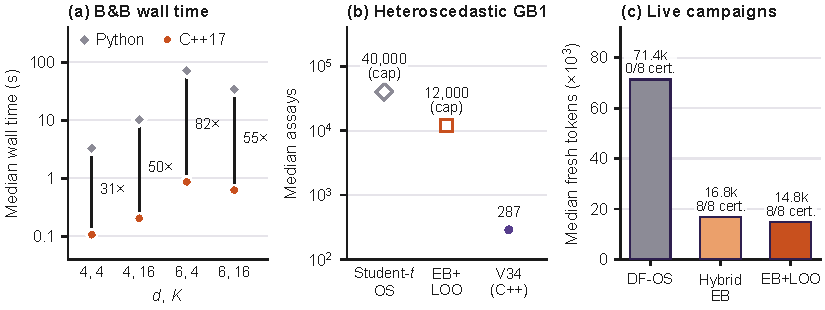
\includegraphics{figures/supp_native_solver_and_workflows.pdf}
\vspace{-12pt}
\caption{\textbf{Native global-solver costs and downstream applications.} (a) Recorded Python and compiled C++17 median wall time for the four paired globally verified branch-and-bound configurations. (b) Median simulated assay count on the fixed-feature projected GB1 task (hollow markers: the median run reached its evaluation cap, $40$k for the Student-$t$ reference and $12$k for EB+LOO). (c) Fresh tokens in the separate eight-campaign Qwen3-0.6B experiment, with DF-OS capped and calibrated EB+LOO completing. Sources: Tables~\ref{tab:app-v10-cpp}, \ref{tab:app-v10-real-v34}, and~\ref{tab:app-v10-live}.}
\label{fig:app-v10}
\end{figure}

\subsection{Independent numerical-oracle verification}
\begin{table}[!htbp]
\caption{\textbf{Independent, zero-shared-code independent numerical-oracle verification audit ($5/5$ PASS in $276.8$ s).} Every core solver in the manuscript is audited against an independent reference implementation (direct \texttt{CVXPY} SOCPs/QPs, \texttt{SciPy differential\_evolution} $+$ dense boundary grids $+$ $50$-digit \texttt{decimal} evaluation, $100{,}000$-draw Monte Carlo null-boundary supermartingale checks, and brute-force DAG dynamic programming).}
\label{tab:app-v11-oracle}
\uniformaligntable{0.93}{%
\begin{tabular}{@{}llrrl@{}}
\toprule
\textbf{Audit / Theorem} & \textbf{Independent Reference} & \textbf{Scale} & \textbf{Violations} & \textbf{Verified Precision / Margin} \\
\midrule
A: Conic Regret (Thm.~\ref{thm:t1-dual}) & Direct \texttt{CVXPY} SOCP & $200$ ($d\in\{2..16\}$) & $\mathbf{0/200}$ sound, $0$ Cara. & SPD $\le 4.30\times 10^{-7}$; sing.\ cons.\ gap $\le .031$ \\
B: Rate $I_*(\theta)$ (Thm.~\ref{thm:bay-main-optimal}) & \texttt{CVXPY} primal QPs $+$ Dirichlet & $100$ DAGs ($648$ QPs) & $\mathbf{0/100}$ dom.\ fails & Dual--primal QP $\le 6.88\times 10^{-6}$ \\
C1: Sparse-KL Nulls (Thm.~\ref{thm:v34-action-local}) & \texttt{diff.\ evol.} $+$ grids $+$ $50$-digit & $500$ rand.\ $+$ $200$ bimodal & $\mathbf{0/700}$ (vs.\ $183/200$ SLSQP) & $50$-digit diff $\le 7.11\times 10^{-15}$ \\
C2: Null Supermartingale & Exact MC ($\sigma_{\max}/\sigma_{\min}\in[1,50]$) & $100{,}000$ draws ($5$ prof.) & $\mathbf{0/5}$ profiles & $\max\widehat{\mathbb E}[F]=.5184\le 1$ (CI95 $\le .5190$) \\
D: Dual Covers (Thm.~\ref{thm:charged-dual-cover}) & Brute-force full-DAG DP & $100$ DAGs ($20{,}000$ steps) & $\mathbf{0/20{,}000}$ mismatches & Max regret diff $=0.0$ \\
\bottomrule
\end{tabular}%
}
\end{table}

\subsection{Independent trajectory and checkpoint verification}
\label{app:trajectory-audit}

To verify Proposition~\ref{prop:ta-coupled} empirically, an external replay audit ran an unmonitored reference TA-UCT allocator alongside all four monitored implementations across the longest observed rollout prefix of every configuration and seed ($911{,}532$ rollouts in the primary suite plus $436{,}096$ rollouts in the gap-intervention study). At every single rollout, the audit verified exact agreement on the selected root-to-leaf path, terminal reward draw, empirical root recommendation, root confidence intervals $[l_t(a), u_t(a)]$, optimistic leader $a_t^*$, and stopping decision. In addition, independent full-DAG reverse-topological dynamic programming checkpoints verified the exact root confidence intervals at initialization, during the first eight rollouts, at every power-of-two rollout, and at termination ($1{,}510$ checkpoints in the primary suite and $456$ in the gap study), with zero discrepancies.

The paired-trajectory and independent-oracle tests support the implementation contracts under the tested conditions. They do not replace the statistical or deterministic proofs. The source archive and its experimental configurations, verification routines, and documented reproducibility limitations are described in the main text.

\end{document}

